% !TEX program = xelatex
\documentclass[12pt,a4paper]{article}
\setcounter{tocdepth}{3}
\setcounter{secnumdepth}{3}
\usepackage{caption}
\captionsetup[table]{position=bottom}
\captionsetup[figure]{position=bottom}
\usepackage{float}
\usepackage{placeins} % \FloatBarrier: hình không trôi qua ranh giới tiểu mục
% Hình được đặt cùng văn bản thay vì dồn sang trang chỉ có hình còn trống nhiều.
\renewcommand{\topfraction}{0.85}
\renewcommand{\bottomfraction}{0.6}
\renewcommand{\textfraction}{0.1}
\renewcommand{\floatpagefraction}{0.75}
\usepackage{fontspec}
% Times New Roman trên máy cá nhân; Overleaf không có font này nên dùng TeX Gyre Termes, bản sao của Times.
\IfFontExistsTF{Times New Roman}{%
  \setmainfont{Times New Roman}%
  \setmonofont{Times New Roman}%
}{%
  \setmainfont{TeX Gyre Termes}%
  \setmonofont{TeX Gyre Termes}%
}
\renewcommand{\figurename}{Hình}
\renewcommand{\tablename}{Bảng}
\renewcommand{\refname}{TÀI LIỆU THAM KHẢO}
\usepackage{tocloft,calc}
\usepackage[top=3.5cm, bottom=3.0cm, left=3.5cm, right=2.0cm]{geometry} % căn lề theo quy chuẩn KLTN
\usepackage{amsmath,latexsym,amscd,amsfonts,mathrsfs,enumerate} \usepackage{ upgreek }
\usepackage[thref,thmmarks,standard,amsmath,hyperref]{ntheorem}
\usepackage[mathscr]{eucal}
\usepackage[unicode,colorlinks=true, bookmarks=true, pdfstartview=FitH,]{hyperref} %pagebackref=true,
\hypersetup{
pdftitle={Hệ thống khuyến nghị sản phẩm điện tử bằng hồi quy lân cận và khuếch tán trên đồ thị},
pdfauthor={Đặng Anh Tuyền;},
colorlinks = true,
linkcolor = black,
citecolor = blue,
urlcolor = blue,
}
\usepackage{fancyhdr}
\usepackage{graphicx}
\graphicspath{{image/}}
\usepackage{fancybox,cite}
\usepackage{subcaption}
\usepackage[ruled,linesnumbered,lined,longend]{algorithm2e}
% Trình bày mã giả: đường dọc theo khối, số dòng nhỏ, dòng tiếp nối thụt vào.
\SetAlFnt{\fontsize{11}{13.5}\selectfont}
\SetAlgoNlRelativeSize{-2}
\SetNlSty{bfseries}{}{}
\SetNlSkip{0.7em}
\SetInd{0.5em}{1.1em}
\SetAlgoHangIndent{1.5em}
\SetAlgoSkip{medskip}
\SetAlCapFnt{\bfseries}
\SetAlCapNameFnt{\bfseries}
\SetAlgorithmName{Thuật toán}{thuật toán}{Danh sách thuật toán}
\SetKwInput{KwIn}{Đầu vào}
\SetKwInput{KwOut}{Đầu ra}
\SetKwFor{For}{với}{thực hiện}{kết thúc}
\SetKwFor{ForEach}{với mỗi}{thực hiện}{kết thúc}
\SetKwFor{While}{trong khi}{thực hiện}{kết thúc}
\SetKwIF{If}{ElseIf}{Else}{nếu}{thì}{ngược lại nếu}{ngược lại}{kết thúc}
%\usepackage{refcheck}
 
\allowdisplaybreaks
%Môi trường định nghĩa
\theoremheaderfont{\bfseries} % In ra chữ "định nghĩa": đậm, thẳng đứng.
\theorembodyfont{} % Nội dung của định nghia được viết bằng chữ thẳng đứng.
\theoremseparator {}         % Ngăn cách giữa định nghĩa và nội dung định nghĩa bởi dấu chấm.
\newtheorem{dn}{Định nghĩa}[section] % Lệnh này để trong file kết quả in ra chữ nhận xét thay vì nếu ta để mặc định.

%Môi trường Ví dụ
\theoremheaderfont{\bfseries} % In ra chữ "Ví dụ": đậm, thẳng đứng.
\theorembodyfont{\normalfont} % Nội dung của ví dụ được viết bằng chữ thẳng đứng.
\theoremseparator {.}         % Ngăn cách giữa Ví dụ và nội dung ví dụ bởi dấu chấm.
\newtheorem{vd}{Ví dụ}[section] % Lệnh này để trong file kết quả in ra chữ Ví dụ thay vì Example nếu ta để mặc định.

%Môi trường Chú ý
\theoremstyle{plain} %Không đánh sỗ chú ý
\theoremheaderfont{\bfseries} % In ra chữ "chú ý": đậm, thẳng đứng.
\theorembodyfont{\normalfont} % Nội dung của chú ý được viết bằng chữ thẳng đứng.
\theoremseparator {}         % Ngăn cách giữa "chú ý" và nội dung chú ý bởi dấu chấm.
\newtheorem{cy}{Chú ý} % Lệnh này để trong file kết quả in ra chữ "chú ý" thay vì remark nếu ta để mặc định.
\usepackage{booktabs}
\usepackage{longtable}
\usepackage{fvextra}
\usepackage{enumitem}
\setlist{itemsep=3pt,topsep=5pt,parsep=0pt}
\usepackage{tabularx}
\usepackage{multirow}
\usepackage{makecell}
\usepackage{tikz}
\usepackage{xurl}

% Khối lệnh cài đặt: phông đơn cách chỉ áp dụng bên trong môi trường này.
% Consolas trên Windows; Overleaf (TeX Live trên Linux) không có nên dùng DejaVu Sans Mono hoặc Latin Modern Mono.
\IfFontExistsTF{Consolas}{%
  \newfontfamily\DemoCommandFont{Consolas}[Scale=MatchLowercase]%
}{%
  \IfFontExistsTF{DejaVu Sans Mono}{%
    \newfontfamily\DemoCommandFont{DejaVu Sans Mono}[Scale=MatchLowercase]%
  }{%
    \newfontfamily\DemoCommandFont{Latin Modern Mono}[Scale=MatchLowercase]%
  }%
}
\definecolor{DemoCommandBackground}{RGB}{247,248,250}
\definecolor{DemoCommandBorder}{RGB}{190,195,202}
\DefineVerbatimEnvironment{DemoCommand}{Verbatim}{%
    fontsize=\small,
    formatcom=\DemoCommandFont,
    baselinestretch=1.15,
    frame=single,
    framerule=0.4pt,
    framesep=7pt,
    rulecolor=\color{DemoCommandBorder},
    bgcolor=DemoCommandBackground,
    breaklines=true,
    breakanywhere=false
}

\Urlmuskip=0mu plus 1mu
\emergencystretch=3em
\usetikzlibrary{arrows.meta,positioning,calc}

% Kiểu dùng chung cho các sơ đồ vector ở Chương 3.
\tikzset{
    chthreeflow/.style={-{Latex[length=2.5mm,width=1.7mm]}, line width=0.9pt, draw=blue!35!black, shorten <=2pt, shorten >=2pt},
    chthreedash/.style={-{Latex[length=2.3mm,width=1.5mm]}, line width=0.85pt, dashed, draw=blue!55!black, shorten <=2pt, shorten >=2pt},
    chthreeblue/.style={draw=blue!70!black, fill=blue!4, rounded corners=5pt, line width=0.8pt, align=center, inner sep=6pt},
    chthreegreen/.style={draw=green!55!black, fill=green!5, rounded corners=5pt, line width=0.8pt, align=center, inner sep=6pt},
    chthreepurple/.style={draw=violet!70!black, fill=violet!5, rounded corners=5pt, line width=0.8pt, align=center, inner sep=6pt},
    chthreeorange/.style={draw=orange!80!black, fill=orange!6, rounded corners=5pt, line width=0.8pt, align=center, inner sep=6pt}
}

% Hiển thị các số phương trình được dẫn lại bằng màu xanh.
\renewcommand{\eqref}[1]{%
    \hyperref[#1]{\textcolor{blue}{\textup{(\ref*{#1})}}}%
}

% Hiển thị số hình được dẫn lại bằng màu xanh, giữ chữ "hình" màu đen.
% \figref viết thường dùng giữa câu; \Figref viết hoa dùng ở đầu câu hoặc đầu ô bảng.
\newcommand{\figref}[1]{%
    hình~\hyperref[#1]{\textcolor{blue}{\ref*{#1}}}%
}
\newcommand{\Figref}[1]{%
    Hình~\hyperref[#1]{\textcolor{blue}{\ref*{#1}}}%
}

% Hiển thị số bảng được dẫn lại bằng màu xanh, giữ chữ "bảng" màu đen.
% \tabref viết thường dùng giữa câu; \Tabref viết hoa dùng ở đầu câu hoặc đầu ô bảng.
\newcommand{\tabref}[1]{%
    bảng~\hyperref[#1]{\textcolor{blue}{\ref*{#1}}}%
}
\newcommand{\Tabref}[1]{%
    Bảng~\hyperref[#1]{\textcolor{blue}{\ref*{#1}}}%
}

% Tô xanh toàn bộ cụm trích dẫn, gồm ngoặc vuông và phần chỉ vị trí (ví dụ [13, Mục 4.4]).
\let\origcite\cite
\renewcommand{\cite}[2][]{{\color{blue}\if\relax\detokenize{#1}\relax\origcite{#2}\else\origcite[#1]{#2}\fi}}

%Môi trường Bài tập
\theoremheaderfont{\bfseries} % In ra chữ "chú ý": đậm, thẳng đứng.
\theorembodyfont{\normalfont} % Nội dung của chú ý được viết bằng chữ thẳng đứng.
\theoremseparator {}         % Ngăn cách giữa "chú ý" và nội dung chú ý bởi dấu chấm.\newtheorem{bt}{Bài tập} % Lệnh này để trong file kết quả in ra chữ "chú ý" thay vì  remark nếu ta để mặc định.

%Môi trường nhân xét
\theoremheaderfont{\bfseries} % In ra chữ "Nhân xét": đậm, thẳng đứng.
\theorembodyfont{\normalfont} % Nội dung của nhạn xét được viết bằng chữ thẳng đứng.
\theoremseparator {}         % Ngăn cách giữa nhận xét và nội dung nhận xét bởi dấu chấm.
\newtheorem{nx}{Nhận xét}[section] % Lệnh này để trong file kết quả in ra chữ nhận xét thay vì nếu ta để mặc định.

%Môi trường định lý
\theoremstyle{plain} %Sử dụng phong cách plain để đánh số Định lý, chẳng hạn: Định lý 1, Định lý 2,...
\theoremheaderfont{\normalfont\bfseries} % In ra chữ "Định lý": đậm, thẳng đứng.
\theorembodyfont{\normalfont} % Nội dung của Định lý được viết bằng chữ nghiêng.
\theoremseparator {.}         % Ngăn cách giữa Định lý và nội dung định lý bởi dấu chấm.
\renewtheorem{theorem}{Định lý} % Lệnh này để trong file kết quả in ra chữ Định lý thay vì theorem nếu ta để mặc định.
%Môi trường Mệnh đề
\theoremstyle{plain} %Sử dụng phong cách plain để đánh số Mệnh đề, chẳng hạn: Mệnh đề 1, Mệnh đề 2,...
\theoremheaderfont{\normalfont\bfseries} % In ra chữ "Mệnh đề": đậm, thẳng đứng.
\theorembodyfont{\normalfont} % Nội dung của Mệnh đề được viết bằng chữ thẳng đứng.
\theoremseparator {.}         % Ngăn cách giữa Mệnh đề và nội dung mệnh đề bởi dấu chấm.
\renewtheorem{proposition}{Mệnh đề}[section] % Lệnh này để trong file kết quả in ra chữ Mệnh đề thay vì proposition nếu ta để mặc định.
%Môi trường Chứng minh
\theoremstyle{nonumberplain}  % Kiểu định dạng dành cho chứng minh
\theoremheaderfont{\normalfont\bfseries} % Tiêu đề "Chứng minh" in nghiêng
\theorembodyfont{\normalfont}
\theoremseparator{.} 
\theoremsymbol{\ensuremath{\square}} % Dấu kết thúc chứng minh là ô vuông
\newtheorem{cm}{Chứng minh}[section]

\pagestyle{fancy}
\fancyhf{}
\fancyhead[L]{\itshape Học máy nâng cao 1-1-26(N01)}
\fancyfoot[L]{\fontsize{9}{11}\selectfont\itshape Hệ thống khuyến nghị sản phẩm điện tử bằng hồi quy lân cận và khuếch tán trên đồ thị}
\fancyfoot[R]{\fontsize{9}{11}\selectfont\thepage}
\setlength{\headheight}{16pt}
\renewcommand{\headrulewidth}{1.2pt}
\renewcommand{\footrulewidth}{1.2pt} % Tiêu đề chân trang
\fancypagestyle{plain}{
    \fancyhf{}
    \fancyhead[L]{\itshape Học máy nâng cao 1-1-26(N01)}
    \fancyfoot[L]{\fontsize{9}{11}\selectfont\itshape Hệ thống khuyến nghị sản phẩm điện tử bằng hồi quy lân cận và khuếch tán trên đồ thị}
    \fancyfoot[R]{\fontsize{9}{11}\selectfont\thepage}
    \renewcommand{\headrulewidth}{1.2pt}
    \renewcommand{\footrulewidth}{1.2pt}
}

\numberwithin{equation}{section}
\numberwithin{figure}{section}
\numberwithin{table}{section}

\begin{document}
 \fontsize{13pt}{18pt}\selectfont
 \hypersetup{pageanchor=false}
 
 \thisfancypage{\setlength{\fboxsep}{0.2cm}\setlength{\fboxrule}{1pt}\doublebox}{}
 \begin{titlepage}
\begin{center}
	\large
	BỘ GIÁO DỤC VÀ ĐÀO TẠO\\
	\textbf{ĐẠI HỌC PHENIKAA}\\
	\textbf{TRƯỜNG CÔNG NGHỆ THÔNG TIN}\\[0.15cm]
	\rule{3.2cm}{0.4pt}\,o0o\,\rule{3.2cm}{0.4pt}
\end{center}
\vspace{-0.5cm}
\begin{center}
    
\includegraphics[scale=0.8]{image/Logo.png}\\[1cm] 
\end{center} 
\vspace{0.3 cm}
\begin{center}
    \bf\Large {BÁO CÁO BÀI TẬP LỚN}
\end{center}
\begin{center}
    \bf\large {HỌC PHẦN: HỌC MÁY NÂNG CAO 1-1-26(N01)}
\end{center}
\vspace{0.3 cm}
\begin{center}
	\bf\large ĐỀ TÀI: HỆ THỐNG KHUYẾN NGHỊ SẢN PHẨM ĐIỆN TỬ BẰNG HỒI QUY LÂN CẬN VÀ KHUẾCH TÁN TRÊN ĐỒ THỊ
\end{center}
\begin{center}
	\normalsize
	\renewcommand{\arraystretch}{1.15}
	\begin{tabular}{@{}p{5.2cm}l@{}}
        \textbf{Đặng Anh Tuyền} & \textbf{MSSV:} 23010912 \\
                                & \textbf{Lớp:} K17-KHMT(AI\&KHDL)\_1 \\[0.25cm]
        \textbf{Phạm Văn Sự} & \textbf{MSSV:} 23010523 \\
                                & \textbf{Lớp:} K17-KHMT(AI\&KHDL)\_1 \\[0.25cm]
        \textbf{Nguyễn Chí Tài} & \textbf{MSSV:} 23010548 \\
                                & \textbf{Lớp:} K17-KHMT(AI\&KHDL)\_1
	\end{tabular}
\end{center}

\vskip 0.8 cm
  \begin{center}
   GVHD: PGS.TS. Phạm Tiến Lâm
  \end{center}
\vskip 0.5 cm
  \begin{center}
   {\large\textbf{Hà Nội, Năm 2026}}
  \end{center}
 \end{titlepage}

% Bìa lót: bố cục học thuật theo mẫu, có khung đôi và không sử dụng logo.
\begin{titlepage}
\thispagestyle{empty}
\thisfancypage{\setlength{\fboxsep}{0.2cm}\setlength{\fboxrule}{1pt}\doublebox}{}
\begin{center}
	\large
	BỘ GIÁO DỤC VÀ ĐÀO TẠO\\
	\textbf{ĐẠI HỌC PHENIKAA}\\
	\textbf{TRƯỜNG CÔNG NGHỆ THÔNG TIN}\\[0.15cm]
	\rule{4cm}{0.4pt}\,o0o\,\rule{4cm}{0.4pt}
\end{center}
\vspace{1.5cm}
\begin{center}
	\normalsize
	\renewcommand{\arraystretch}{1.15}
	\begin{tabular}{@{}p{5.2cm}l@{}}
        \textbf{Đặng Anh Tuyền} & \textbf{MSSV:} 23010912 \\
                                & \textbf{Lớp:} K17-KHMT(AI\&KHDL)\_1 \\[0.25cm]
        \textbf{Phạm Văn Sự} & \textbf{MSSV:} 23010523 \\
                                & \textbf{Lớp:} K17-KHMT(AI\&KHDL)\_1 \\[0.25cm]
        \textbf{Nguyễn Chí Tài} & \textbf{MSSV:} 23010548 \\
                                & \textbf{Lớp:} K17-KHMT(AI\&KHDL)\_1
	\end{tabular}
\end{center}
\vspace{1.3cm}
\begin{center}
    \bf\Large {BÁO CÁO BÀI TẬP LỚN}
\end{center}
\begin{center}
    \bf\large {HỌC PHẦN: HỌC MÁY NÂNG CAO 1-1-26(N01)}
\end{center}
\vspace{0.65cm}
\begin{center}
	\bf\Large HỆ THỐNG KHUYẾN NGHỊ SẢN PHẨM ĐIỆN TỬ BẰNG HỒI QUY LÂN CẬN VÀ KHUẾCH TÁN TRÊN ĐỒ THỊ
\end{center}
\vfill
\begin{center}
    GVHD: PGS.TS. Phạm Tiến Lâm
\end{center}
\vfill
\begin{center}
    {\large\textbf{Hà Nội, Năm 2026}}
\end{center}
\vspace{0.25cm}
\end{titlepage}

% Bảng phân chia công việc của nhóm.
\begin{titlepage}
\thispagestyle{empty}
\begin{center}
    {\bfseries\Large BẢNG PHÂN CHIA CÔNG VIỆC}
\end{center}
\vspace{0.45cm}

\begingroup
\fontsize{10.5pt}{12.5pt}\selectfont
\setlength{\tabcolsep}{3.5pt}
\setlength{\arrayrulewidth}{0.7pt}
\renewcommand{\arraystretch}{1.08}
\begin{center}
\begin{tabularx}{\textwidth}{|
    >{\centering\arraybackslash}m{0.8cm}|
    >{\centering\arraybackslash}m{3.5cm}|
    >{\centering\arraybackslash}p{1.75cm}|
    >{\raggedright\arraybackslash}X|
    >{\centering\arraybackslash}m{1.45cm}|}
\hline
\textbf{STT} & \centering\textbf{Họ và tên} & \textbf{Vai trò} & \centering\textbf{Nội dung công việc} & \textbf{Tỷ lệ} \\
\hline
1 & \makecell[c]{Đặng Anh Tuyền} & Trưởng nhóm &
\begin{minipage}[t]{\linewidth}\raggedright\begin{itemize}[nosep,leftmargin=1.1em]
\item Điều phối nhóm
\item Tiền xử lý dữ liệu và chia tập theo thời gian
\item Tạo các mức giảm dữ liệu huấn luyện
\item Đề xuất và cài đặt GRNR
\item Cài đặt EASE và GF-CF
\item Tham gia xây dựng báo cáo và slide
\end{itemize}\vspace{3pt}\end{minipage} & 33\% \\
\hline
2 & \makecell[c]{Phạm Văn Sự} & Thành viên &
\begin{minipage}[t]{\linewidth}\raggedright\begin{itemize}[nosep,leftmargin=1.1em]
\item Đề xuất và cài đặt DFHF
\item Cài đặt LightGCN, XSimGCL và \mbox{DirectAU}
\item Huấn luyện các mô hình nhóm cần huấn luyện trên Kaggle
\item Tham gia xây dựng báo cáo và slide
\end{itemize}\vspace{3pt}\end{minipage} & 33\% \\
\hline
3 & \makecell[c]{Nguyễn Chí Tài} & Thành viên &
\begin{minipage}[t]{\linewidth}\raggedright\begin{itemize}[nosep,leftmargin=1.1em]
\item Xây dựng giao thức đánh giá
\item Cài đặt kiểm định bootstrap ghép cặp
\item Phân tích kết quả và vẽ biểu đồ
\item Xây dựng hệ thống demo
\item Tham gia xây dựng báo cáo và slide
\end{itemize}\vspace{3pt}\end{minipage} & 33\% \\
\hline
\end{tabularx}
\end{center}
\endgroup

\vspace{0.5cm}
{\fontsize{12pt}{15pt}\selectfont
\noindent\textbf{Công khai sử dụng công cụ AI.} Nhóm sử dụng trợ lý AI Claude của Anthropic để:
\begin{itemize}[nosep,leftmargin=1.5em]
\item gợi ý chọn hướng đề tài hệ thống khuyến nghị;
\item hỗ trợ tìm hiểu tài liệu và quy trình xây dựng dự án;
\item thiết kế giao diện và trải nghiệm người dùng của ứng dụng demo;
\item rà soát tính nhất quán giữa văn bản, bảng và hình;
\item hỗ trợ kiểm tra và sửa lỗi mã nguồn của dự án.
\end{itemize}
\vspace{0.3cm}
\noindent\textbf{Phần tự cài đặt và phần kế thừa.} Không dùng thư viện khuyến nghị dựng sẵn:
\begin{itemize}[nosep,leftmargin=1.5em]
\item GRNR và DFHF do nhóm tự thiết kế và cài đặt;
\item EASE, GF-CF, LightGCN, XSimGCL và DirectAU được cài lại theo bài báo gốc và mã của tác giả;
\item tiền xử lý, đánh giá, kiểm định và demo do nhóm tự viết trên PyTorch, NumPy, SciPy và Streamlit.
\end{itemize}
\vspace{0.3cm}
\noindent\textbf{Giấy phép dữ liệu.} Bộ dữ liệu đánh giá sản phẩm Amazon được McAuley và cộng sự công bố công khai cho mục đích nghiên cứu~\cite{mcauley2015image,he2016ups}; nhóm chỉ dùng dữ liệu cho mục đích học thuật và không phân phối lại dữ liệu gốc.\par}

\vspace{0.7cm}
\begin{center}
    {\fontsize{13pt}{16pt}\selectfont
    \textbf{Repository dự án:}\quad
    \href{https://github.com/tuyenda2011/GRNR-DFHF-RecSys}{\texttt{github.com/tuyenda2011/GRNR-DFHF-RecSys}}}
\end{center}
\end{titlepage}

\pagestyle{fancy}
\pagenumbering{arabic}
\setcounter{page}{1}
\hypersetup{pageanchor=true,linkcolor=black}

% Chèn mục lục
\renewcommand{\contentsname}{Mục lục}
\tableofcontents

% Ngắt trang tại đây để chuyển Danh mục hình ảnh sang trang mới
\newpage 
%\clearpage % (Bạn cũng có thể dùng \clearpage thay cho \newpage)

% Chèn danh mục hình ảnh
\renewcommand{\listfigurename}{Danh sách hình ảnh}
\listoffigures

% Chèn danh mục bảng
\clearpage
\renewcommand{\listtablename}{Danh sách bảng}
\listoftables

% Danh mục từ viết tắt
\clearpage
\section*{Danh mục từ viết tắt}
\addcontentsline{toc}{section}{Danh mục từ viết tắt}
\begingroup
\renewcommand{\arraystretch}{1.15}
\begin{longtable}{@{}l>{\raggedright\arraybackslash}p{0.72\linewidth}@{}}
\toprule
Viết tắt & Tên đầy đủ hoặc ý nghĩa \\
\midrule
\endhead
BPR & Bayesian Personalized Ranking, hàm mất mát xếp hạng theo cặp \\
BSPM & Blurring-Sharpening Process Models, mô hình lọc đồ thị gần đây, không chạy trong thực nghiệm \\
CPU, GPU & Central Processing Unit (bộ xử lý trung tâm), Graphics Processing Unit (bộ xử lý đồ họa) \\
DCG & Discounted Cumulative Gain, tổng lợi ích chiết khấu theo vị trí \\
IDCG & Ideal Discounted Cumulative Gain, giá trị DCG của thứ tự lý tưởng \\
DFHF & Diffusion-Filtered History Factorization, mô hình đề xuất thuộc nhóm cần huấn luyện \\
DirectAU & Tên riêng, bài gốc không nêu dạng đầy đủ; hàm mục tiêu tối ưu trực tiếp tính căn chỉnh (alignment) và tính đồng đều (uniformity), baseline thuộc nhóm cần huấn luyện \\
EASE & Embarrassingly Shallow Autoencoder, baseline thuộc nhóm giải trực tiếp \\
FISM & Factored Item Similarity Models \\
GF-CF & Graph Filter based Collaborative Filtering, baseline thuộc nhóm giải trực tiếp \\
GRNR & Graph-Regularized Neighborhood Regression, mô hình đề xuất thuộc nhóm giải trực tiếp \\
KTC & Khoảng tin cậy \\
LightGCN & Light Graph Convolution Network, baseline thuộc nhóm cần huấn luyện \\
GiB & Gibibyte ($2^{30}$ byte) \\
MiB & Mebibyte ($2^{20}$ byte) \\
MostPop & Xếp hạng theo độ phổ biến, mốc tham chiếu không cá nhân hóa \\
Mult-VAE & Variational Autoencoder với phân phối đa thức \\
NDCG@$K$ & Normalized Discounted Cumulative Gain at $K$ \\
Recall@$K$ & Recall at $K$, tỉ lệ sản phẩm mục tiêu nằm trong $K$ vị trí đầu \\
SLIM & Sparse Linear Methods \\
XSimGCL & eXtremely Simple Graph Contrastive Learning, baseline thuộc nhóm cần huấn luyện \\
\bottomrule
\end{longtable}
\endgroup

% Danh mục ký hiệu
\clearpage
\section*{Danh mục ký hiệu}
\addcontentsline{toc}{section}{Danh mục ký hiệu}
Bảng dưới liệt kê các ký hiệu dùng xuyên suốt báo cáo. Ký hiệu chỉ dùng trong một công thức được giải thích ngay tại chỗ.

\begingroup
\fontsize{12}{15}\selectfont
\renewcommand{\arraystretch}{1.00}
\begin{longtable}{@{}l>{\raggedright\arraybackslash}p{0.56\linewidth}l@{}}
\toprule
Ký hiệu & Ý nghĩa & Định nghĩa \\
\midrule
\endhead
$\mathcal{U}$, $\mathcal{I}$ & Tập người dùng, tập sản phẩm & Mục~\ref{sec:notation} \\
$X$ & Ma trận tương tác nhị phân, $X_{ui}=1$ nếu đã quan sát được tương tác & Định nghĩa~\ref{def:implicit} \\
$x_u$ & Hàng $u$ của $X$, tức lịch sử của người dùng $u$ dưới dạng vector & Mục~\ref{sec:notation} \\
$H_u$, $n_u$ & Lịch sử của người dùng $u$ và độ dài lịch sử & Mục~\ref{sec:notation} \\
$c_i$ & Số người dùng đã tương tác với sản phẩm $i$ (độ phổ biến) & Mục~\ref{sec:notation} \\
$D_U$, $D_I$ & Ma trận bậc của người dùng và của sản phẩm & Mục~\ref{sec:notation} \\
$E$, $|E|$ & Tập tương tác và số tương tác & Mục~\ref{sec:notation} \\
$s(u,i)$ & Điểm mô hình gán cho cặp $(u,i)$ & Định nghĩa~\ref{def:topk} \\
$\mathcal{C}_u$ & Tập sản phẩm ứng viên hợp lệ của người dùng $u$ & Định nghĩa~\ref{def:topk} \\
$K$ & Số sản phẩm trong danh sách gợi ý & Định nghĩa~\ref{def:topk} \\
$f$ & Số chiều embedding & Mục~\ref{sec:trained-models} \\
$\lambda$ & Hệ số phạt ridge của EASE & Mục~\ref{sec:ease} \\
$\kappa_{\mathrm{lift}}$ & Hằng số làm trơn điểm dư đồng xuất hiện của GRNR & \eqref{eq:grnr-lift} \\
$\omega_+$ & Trọng số mẫu dương của GRNR & \eqref{eq:grnr-objective} \\
$\rho_{\mathrm{pop}}$ & Số mũ điều chỉnh độ phổ biến của GRNR & Mục~\ref{sec:grnr-algorithm} \\
$\lambda_{\mathrm{emb}}$ & Hệ số phạt ridge cho embedding của DFHF & \eqref{eq:dfhf-objective} \\
$\Omega$, $P$ & Ma trận trọng số mẫu, ma trận phạt trong hồi quy có trọng số & Định nghĩa~\ref{def:wls} \\
$C$, $C^\circ$ & Ma trận đồng xuất hiện và phiên bản có đường chéo bằng 0 & Mục~\ref{sec:notation}, Định nghĩa~\ref{def:cooccurrence} \\
$A$, $D_A$ & Ma trận kề của một đồ thị và ma trận bậc của nó & Định nghĩa~\ref{def:laplacian} \\
$\tilde A$, $L$ & Ma trận kề chuẩn hóa, Laplacian chuẩn hóa & Định nghĩa~\ref{def:laplacian} \\
$T$ & Ma trận chuyển hai bước sản phẩm $\to$ người dùng $\to$ sản phẩm & \eqref{eq:transition} \\
$\mathcal{B}$ & Ma trận hệ số sản phẩm--sản phẩm của GRNR & Mục~\ref{sec:grnr-algorithm} \\
$S$, $V$ & Hai bảng embedding nguồn và đích của DFHF & Mục~\ref{sec:dfhf-representation} \\
$b$, $b_i$ & Vector chặn theo sản phẩm và phần tử thứ $i$; dùng ở cả GRNR và DFHF, mỗi mô hình học vector riêng & Mục~\ref{sec:grnr-algorithm}, \ref{sec:dfhf-representation} \\
$Q_{\mathrm{batch}}$ & Số truy vấn tối đa trong một lô huấn luyện của DFHF & Mục~\ref{sec:dfhf-algorithm} \\
$F$, $\pi_i$ & Bộ lọc khuếch tán và xác suất sản phẩm $i$ được lấy làm đích & Mục~\ref{sec:dfhf-representation}, \ref{sec:dfhf-objective} \\
$\mathcal{Q}$ & Lô, tập tương tác dùng trong một bước cập nhật & Mục~\ref{sec:trained-models} \\
$\mathbb{E}$ & Kỳ vọng & Mục~\ref{sec:cooccurrence} \\
$d$ & Tỉ lệ tương tác huấn luyện được giữ lại & Mục~\ref{sec:sparsity-protocol} \\
\bottomrule
\end{longtable}
\endgroup

% Ngắt trang để phần nội dung bài viết bắt đầu ở trang mới
\clearpage
% Tóm tắt
\section*{\centering Tóm tắt}
\addcontentsline{toc}{section}{Tóm tắt}
Đề tài xét bài toán khuyến nghị top-$K$ từ phản hồi ngầm trên danh mục Electronics của bộ dữ liệu đánh giá sản phẩm Amazon, gồm 124.895 người dùng, 44.843 sản phẩm và khoảng 1,07 triệu tương tác. Nhóm đề xuất hai mô hình biểu diễn người dùng bằng lịch sử tương tác, nhờ đó chấm điểm được lịch sử mới mà không cần huấn luyện lại. Graph-Regularized Neighborhood Regression (GRNR) giải cho mỗi sản phẩm một bài toán hồi quy có điều chuẩn đồ thị trên tối đa 128 láng giềng; Diffusion-Filtered History Factorization (DFHF) học hai bảng embedding sản phẩm được làm trơn bằng bộ lọc khuếch tán và huấn luyện bằng softmax trên toàn danh mục. Mỗi mô hình chỉ được so với ba baseline cùng nhóm, ở bốn mức giữ lại dữ liệu huấn luyện, và được đối chiếu với mốc gợi ý theo độ phổ biến MostPop.

Trên tập kiểm tra độc lập và với toàn bộ dữ liệu huấn luyện, GRNR đạt Normalized Discounted Cumulative Gain tại 20 vị trí đầu (NDCG@20) bằng 0,02843. Kết quả này chưa phân biệt được với Embarrassingly Shallow Autoencoder (EASE) đầy đủ, trong khi dung lượng của GRNR nhỏ hơn khoảng 190 lần. DFHF dẫn đầu nhóm cần huấn luyện ở cả bốn mức dữ liệu, đạt 0,02724 ở mức đầy đủ. Khi bớt dữ liệu, lợi thế cá nhân hóa mất nhanh: còn 50\% tương tác thì mọi mô hình trừ DFHF đã thấp hơn MostPop, còn 25\% thì DFHF chỉ ngang MostPop và các mô hình khác thấp hơn rõ. Trên dữ liệu này, khả năng cá nhân hóa phụ thuộc vào độ dày dữ liệu nhiều hơn vào lựa chọn mô hình. Các kết quả được đo với một seed, sau khi chọn cấu hình và checkpoint trên tập xác thực.

\medskip
\noindent Từ khóa: hệ thống khuyến nghị, phản hồi ngầm, hồi quy lân cận, lọc khuếch tán trên đồ thị, dữ liệu thưa.

\clearpage

\section{Giới thiệu}
\label{sec:intro}

\subsection{Bối cảnh và động cơ}
\label{sec:intro-context}

Một sàn thương mại điện tử có từ hàng chục nghìn đến hàng triệu sản phẩm, trong khi mỗi người dùng chỉ biết đến một phần rất nhỏ trong số đó. Hệ thống khuyến nghị thu hẹp khoảng cách này bằng một danh sách ngắn gồm những sản phẩm người dùng nhiều khả năng quan tâm. Báo cáo xét dạng phổ biến nhất của bài toán, gọi là \emph{khuyến nghị top-$K$}: dựa vào lịch sử của một người dùng, mô hình xếp hạng các sản phẩm người đó chưa tương tác rồi chọn ra $K$ sản phẩm đứng đầu.

Trong phần lớn hệ thống thực tế, ta không có điểm số của người dùng cho từng sản phẩm. Thứ hệ thống thường biết chỉ là người dùng đã mua, đã xem hay đã đánh giá tốt những sản phẩm nào. Dữ liệu kiểu này gọi là \emph{phản hồi ngầm}~\cite{hu2008wmf}, và nó mơ hồ ở một điểm cơ bản: một sản phẩm chưa được tương tác có thể là sản phẩm người dùng không thích, nhưng cũng có thể chỉ là sản phẩm họ chưa từng thấy. Phương pháp nào cũng phải xử lý sự mơ hồ này, hoặc bằng cách tin các ô có tương tác hơn các ô trống~\cite{hu2008wmf}, hoặc bằng cách chỉ học thứ tự giữa sản phẩm đã và chưa tương tác~\cite{rendle2009bpr}.

Nhóm sử dụng danh mục Electronics trong bộ dữ liệu đánh giá sản phẩm Amazon của McAuley và cộng sự~\cite{mcauley2015image,he2016ups}. Bộ dữ liệu công khai, được dùng rộng rãi trong nghiên cứu, và có thời điểm của từng đánh giá nên chia được tập theo thứ tự thời gian. Dữ liệu ghi số sao từ 1 đến 5, nhưng nhóm chỉ giữ lại một thông tin: người dùng có đánh giá tốt sản phẩm hay không. Đánh giá từ 4 sao trở lên được coi là một tương tác, còn mức sao cụ thể bị bỏ. Bài toán top-$K$ chỉ cần biết người dùng quan tâm đến sản phẩm nào, và cách làm này cho mọi mô hình cùng một dạng đầu vào; cái giá là những đánh giá thấp không được dùng đến. Vì thế, ``tương tác'' trong báo cáo là một đánh giá tích cực công khai, không phải một lượt mua. Sau tiền xử lý, dữ liệu còn 124.895 người dùng, 44.843 sản phẩm và khoảng 1,07 triệu tương tác.

\subsection{Thách thức của bài toán}
\label{sec:intro-challenges}

Dữ liệu này có ba đặc điểm chi phối cách xây dựng mô hình, và việc đánh giá mô hình trên nó cũng có những cạm bẫy riêng.

Trước hết, dữ liệu rất thưa. Chỉ khoảng 0,02\% số ô của ma trận tương tác khác 0, và một nửa số người dùng có không quá 6 tương tác. Mỗi người dùng chỉ để lại vài manh mối về sở thích, nên một biểu diễn học riêng cho từng người rất dễ bị nhiễu chi phối. Trường hợp khó nhất là khi người dùng chỉ còn đúng một tương tác, và nhóm xem xét kỹ trường hợp này khi giảm dần dữ liệu huấn luyện.

Đặc điểm thứ hai là lịch sử của người dùng luôn thay đổi. Nhiều mô hình phổ biến, như phân rã ma trận~\cite{koren2009mf} hay các mô hình đồ thị kiểu Light Graph Convolution Network (LightGCN)~\cite{he2020lightgcn}, gán cho mỗi người dùng một vector riêng học trong lúc huấn luyện. Khi người dùng có thêm tương tác, hoặc khi có người dùng mới, vector đó không còn đúng nữa và chỉ cập nhật được bằng cách huấn luyện lại. Ngược lại, có những mô hình tính điểm của một sản phẩm trực tiếp từ các sản phẩm trong lịch sử, chẳng hạn các mô hình láng giềng sản phẩm~\cite{sarwar2001itembased,ning2011slim,steck2019ease} hay Factored Item Similarity Models (FISM)~\cite{kabbur2013fism}. Những mô hình này chấm được một lịch sử mới ngay lập tức. Đây là một tính chất có lợi khi triển khai, có được nhờ thiết kế và được minh họa trong ứng dụng demo, nhưng báo cáo không đo lợi ích của nó bằng số liệu. Điều được đánh giá là mặt trái của lựa chọn này: khi người dùng được biểu diễn hoàn toàn bằng lịch sử, chất lượng phụ thuộc vào việc lịch sử có đủ dài hay không, mà dữ liệu thưa thì không bảo đảm điều đó.

Đặc điểm thứ ba là độ phổ biến tự nó đã là một đối thủ mạnh. Trong thương mại điện tử, một số ít sản phẩm chiếm phần lớn tương tác: ở tập huấn luyện của dự án, 1\% sản phẩm phổ biến nhất chiếm 19,2\% số tương tác, còn 10\% phổ biến nhất chiếm tới 51,8\%. Chỉ cần gợi ý những sản phẩm phổ biến nhất (MostPop) cũng đã đạt một mức chất lượng đáng kể, và Dacrema cùng cộng sự cho thấy nhiều mô hình mạng nơ-ron đã công bố không vượt được các phương pháp đơn giản nếu những phương pháp này được thiết lập cẩn thận~\cite{dacrema2019progress}. Trong các công trình nhóm đã đọc, mô hình mới thường chỉ được so với các mô hình khác; khoảng cách giữa mô hình và cách gợi ý theo độ phổ biến, cùng sự thay đổi của khoảng cách đó khi dữ liệu thưa dần, hiếm khi được báo cáo riêng. Đây là trục chính trong phần đánh giá độ thưa của báo cáo.

Bên cạnh ba đặc điểm trên, việc đánh giá có ba cạm bẫy đã được ghi nhận:
\begin{itemize}
\item thước đo tính trên một mẫu nhỏ sản phẩm âm có thể đảo thứ tự giữa các mô hình~\cite{krichene2020sampled};
\item cách chia dữ liệu và cách chọn siêu tham số có thể làm thay đổi kết luận~\cite{sun2020rigorous};
\item chia tập không theo thứ tự thời gian có thể làm lộ thông tin của tương lai~\cite{ji2023leakage}.
\end{itemize}
Giao thức đánh giá của dự án được thiết kế để tránh hoặc giảm nhẹ từng cạm bẫy này.

\subsection{Hướng tiếp cận}
\label{sec:intro-approach}

Theo cách học tham số, các mô hình khuyến nghị dựa trên phản hồi ngầm chia thành hai nhóm.

Nhóm giải trực tiếp tính tham số bằng một công thức đóng hoặc một phép lọc tuyến tính, không có vòng lặp huấn luyện, và mọi mô hình trong nhóm đều biểu diễn người dùng bằng lịch sử. Hai đại diện tiêu biểu là Embarrassingly Shallow Autoencoder (EASE)~\cite{steck2019ease} và Graph Filter based Collaborative Filtering (GF-CF)~\cite{shen2021gfcf}. Hướng này vẫn đang phát triển: các công trình gần đây như Blurring-Sharpening Process Models (BSPM)~\cite{choi2023bspm} và Turbo-CF~\cite{park2024turbocf} tiếp tục khai thác đồ thị giữa các sản phẩm để giữ chất lượng với chi phí tính toán thấp hơn.

Nhóm cần huấn luyện học embedding, tức vector biểu diễn của sản phẩm và thường của cả người dùng, bằng tối ưu theo gradient qua nhiều epoch. LightGCN, eXtremely Simple Graph Contrastive Learning (XSimGCL)~\cite{yu2023xsimgcl} và DirectAU~\cite{wang2022directau} đều thuộc nhóm này; trong báo cáo, DirectAU được ghép với bộ mã hóa của LightGCN. Cả ba đều dùng vector riêng cho từng người dùng.

Nếu đem một mô hình giải trực tiếp so với một mô hình cần huấn luyện, rất khó biết chênh lệch đến từ đâu, vì hai bên khác nhau cả về chi phí, cách tinh chỉnh lẫn phần cứng phù hợp. Vì vậy nhóm đề xuất một mô hình cho mỗi nhóm và chỉ so mô hình đó với các baseline (mô hình đối chứng) cùng nhóm. Hai mô hình đề xuất được đánh giá độc lập, không so với nhau.

Graph-Regularized Neighborhood Regression (GRNR) thuộc nhóm giải trực tiếp và xuất phát từ một câu hỏi thực dụng. EASE thường là một baseline rất mạnh nhưng cần một ma trận trọng số đầy đủ, có kích thước bằng bình phương số sản phẩm. Liệu có thể thay ma trận đó bằng một số ít láng giềng được ước lượng cẩn thận mà không mất chất lượng? GRNR giải một bài toán hồi quy nhỏ cho mỗi sản phẩm, chỉ trên tối đa 128 sản phẩm láng giềng, với trọng số dành cho dữ liệu ngầm và điều chuẩn theo đồ thị giữa các láng giềng. Với 44.843 sản phẩm của dự án, ma trận đầy đủ của EASE chiếm khoảng 7,5 GiB và vẫn chạy được, nên lợi ích về bộ nhớ của GRNR mới chỉ là dự phóng cho những danh mục lớn hơn. Điều kiểm chứng được trên dữ liệu này là chất lượng: GRNR có giữ được chất lượng của EASE đầy đủ khi chỉ dùng một phần nhỏ số hệ số hay không.

Diffusion-Filtered History Factorization (DFHF) thuộc nhóm cần huấn luyện. Khác với ba baseline cùng nhóm, DFHF không có vector người dùng: mỗi người dùng được mô tả bằng embedding của các sản phẩm trong lịch sử, theo hướng của FISM~\cite{kabbur2013fism}. Hai bảng embedding sản phẩm được làm trơn bằng một bộ lọc khuếch tán trên đồ thị người dùng--sản phẩm, để một sản phẩm ít tương tác mượn được thông tin từ những sản phẩm mà cùng nhóm người dùng đã tương tác. Mô hình được huấn luyện bằng softmax trên toàn bộ danh mục, tức so sản phẩm đúng với mọi sản phẩm ứng viên cùng lúc~\cite{liang2018multvae}. Lựa chọn này lấy động cơ từ phân tích của Wu và cộng sự về softmax lấy mẫu: hàm mất mát này gắn với việc tối đa hóa thước đo xếp hạng, còn phép lan truyền trên đồ thị bù được điểm yếu của nó trong việc điều chỉnh độ lớn của vector biểu diễn~\cite{wu2024sampledsoftmax}. Vì DFHF dùng softmax trên toàn danh mục chứ không lấy mẫu, phân tích này chỉ là cơ sở thiết kế, không phải một bảo đảm cho mô hình. Câu hỏi với DFHF là một mô hình như vậy có cạnh tranh được với các mô hình đồ thị dùng vector người dùng hay không.

Dữ liệu gốc đã qua bộ lọc 5-core, tức chỉ giữ những người dùng và sản phẩm có ít nhất 5 đánh giá, nên dày hơn dữ liệu của một hệ thống thực tế. Để xét những mức thưa gần thực tế hơn, nhóm giảm tập huấn luyện xuống còn 75\%, 50\% và 25\% số tương tác rồi đánh giá lại mọi mô hình. Ở mỗi mức, kết quả được đặt cạnh MostPop để xem mô hình còn hơn cách gợi ý theo độ phổ biến bao nhiêu khi dữ liệu thưa dần. Cách giảm ngẫu nhiên này chỉ mô phỏng độ thưa, không tái hiện đúng tình huống người dùng mới: mọi người dùng vẫn giữ ít nhất một tương tác, và người dùng nhiều tương tác mất nhiều dữ liệu hơn người dùng ít tương tác.

Dự án có ba đóng góp. Thứ nhất là hai mô hình biểu diễn người dùng bằng lịch sử, mỗi mô hình cho một nhóm phương pháp, đều chấm được lịch sử mới mà không cần huấn luyện lại. Thứ hai là một đánh giá có kiểm soát trong từng nhóm, với cùng tập ứng viên, cùng người dùng, bốn mức thưa, kiểm định thống kê ghép cặp theo từng người dùng và đối chiếu có hệ thống với MostPop. Thứ ba là một kho dự án lưu mã nguồn, cấu hình và kết quả của các lần chạy, kèm một ứng dụng demo cho phép thử gợi ý với lịch sử tùy ý. Cả hai mô hình được ghép từ những thành phần đã biết. Trong các tài liệu nhóm đã đọc, chưa thấy công trình nào kết hợp đúng các thành phần này (Mục~\ref{sec:closed-form-gap} và Mục~\ref{sec:trained-gap}), nhưng nhóm không cho rằng đây là những phương pháp hoàn toàn mới.

\subsection{Câu hỏi nghiên cứu và phạm vi}
\label{sec:intro-rq}

Mục tiêu của đề tài là xây dựng hai mô hình khuyến nghị biểu diễn người dùng bằng lịch sử, mỗi mô hình cho một nhóm phương pháp, và đánh giá chúng một cách có kiểm soát, nhất là khi dữ liệu thưa dần. Thước đo chính là Normalized Discounted Cumulative Gain tại 20 vị trí đầu (NDCG@20), cho biết sản phẩm người dùng thực sự tương tác tiếp theo có nằm trong 20 gợi ý đầu hay không và nằm ở vị trí nào. Báo cáo trả lời bốn câu hỏi:
\begin{enumerate}
\item Trong nhóm của mình, mỗi mô hình đề xuất có NDCG@20 cao hơn các baseline cùng nhóm không, và chênh lệch có vượt khỏi biến động theo người dùng không?
\item Khi chỉ giữ lại 75\%, 50\% hoặc 25\% tương tác huấn luyện, chất lượng của mỗi mô hình thay đổi thế nào so với các baseline cùng nhóm và so với MostPop?
\item Chi phí tính toán của mỗi mô hình, gồm thời gian huấn luyện, thời gian suy luận và dung lượng lưu trữ, so với nhóm của nó ra sao?
\item Hai mô hình phục vụ một lịch sử mới như thế nào khi triển khai, và điểm số của GRNR có phân rã được thành lý do gợi ý hay không?
\end{enumerate}

Phạm vi của báo cáo có những giới hạn rõ ràng:
\begin{itemize}
% \item Chất lượng được đo bằng thước đo xếp hạng ngoại tuyến; báo cáo không đánh giá doanh thu, mức hài lòng hay hành vi của người dùng thật.
\item Mọi kết quả đánh giá cuối cùng được đo trên tập kiểm tra độc lập (test set) của một bộ dữ liệu, với một seed (giá trị khởi tạo bộ sinh số ngẫu nhiên), và chỉ trên những người dùng có sản phẩm mục tiêu nằm trong tập ứng viên. Tập xác thực (validation set) chỉ được sử dụng để lựa chọn siêu tham số và checkpoint, không tham gia vào quá trình đánh giá cuối cùng.
\item Câu hỏi thứ tư được trả lời bằng mô tả hệ thống và một ví dụ minh họa, không bằng phép đo định lượng.
% \item Các câu hỏi được chốt sau khi đã có kết quả thực nghiệm, và MostPop được bổ sung trong lúc phân tích. Vì vậy mọi phân tích, kể cả các so sánh với MostPop, đều mang tính khám phá chứ không phải kiểm định một giả thuyết đặt ra từ trước, và kết luận cần được xác nhận trên dữ liệu chưa dùng để chọn cấu hình.
\item Các câu hỏi nghiên cứu và phép so sánh với MostPop được hoàn thiện trong quá trình phân tích thực nghiệm. Vì vậy, các phân tích vẫn mang tính khám phá, chưa phải kiểm định những giả thuyết được xác lập hoàn toàn từ trước. Kết quả cuối cùng được đánh giá trên tập kiểm tra độc lập sau khi cố định cấu hình và checkpoint của các mô hình.
\end{itemize}

\clearpage
\section{Cơ sở lý thuyết và nghiên cứu liên quan}
\label{sec:background}

\subsection{Phát biểu bài toán và ký hiệu}
\label{sec:notation}

\begin{dn}[Dữ liệu phản hồi ngầm]
\label{def:implicit}
Cho tập người dùng $\mathcal{U}$ và tập sản phẩm $\mathcal{I}$. Phản hồi ngầm được biểu diễn bằng ma trận nhị phân $X\in\{0,1\}^{|\mathcal{U}|\times|\mathcal{I}|}$, trong đó $X_{ui}=1$ nếu dữ liệu ghi nhận một tương tác được xem là tích cực giữa người dùng $u$ và sản phẩm $i$, và $X_{ui}=0$ nếu chưa ghi nhận tương tác như vậy.
\end{dn}

Các đại lượng sau được dùng trong toàn báo cáo:
\begin{itemize}
\item $x_u\in\{0,1\}^{|\mathcal{I}|}$ là hàng $u$ của $X$, tức lịch sử của người dùng $u$ dưới dạng vector;
\item $H_u=\{i: X_{ui}=1\}$ là lịch sử của người dùng $u$, và $n_u=|H_u|$ là độ dài lịch sử;
\item $c_i=\sum_{u}X_{ui}$ là số người dùng đã tương tác với sản phẩm $i$, gọi là độ phổ biến của $i$;
\item $C_{ji}=\sum_u X_{uj}X_{ui}$ là số người dùng chung của hai sản phẩm $j$ và $i$;
\item $D_U=\mathrm{diag}(n_u)$ và $D_I=\mathrm{diag}(c_i)$ là ma trận đường chéo chứa độ dài lịch sử và độ phổ biến;
\item $E=\{(u,i): X_{ui}=1\}$ là tập tương tác, $|E|$ là số tương tác.
\end{itemize}
Các lũy thừa nghịch đảo của $D_U$ và $D_I$ chỉ xét trên những người dùng và sản phẩm có ít nhất một tương tác.

\begin{dn}[Bài toán khuyến nghị top-$K$]
\label{def:topk}
Một mô hình khuyến nghị là một hàm điểm $s:\mathcal{U}\times\mathcal{I}\to\mathbb{R}$. Cho tập ứng viên $\mathcal{C}_u\subseteq\mathcal{I}\setminus H_u$ và số nguyên $1\le K\le|\mathcal{C}_u|$, danh sách top-$K$ của người dùng $u$ gồm $K$ phần tử của $\mathcal{C}_u$ có điểm lớn nhất, xếp theo điểm giảm dần.
\end{dn}

Bài toán có hai đặc điểm mà phương pháp nào cũng phải tính đến. Thứ nhất, một ô $X_{ui}=0$ chưa đủ để nói người dùng không thích sản phẩm, vì có thể họ chưa biết hoặc chưa có dịp tương tác với nó~\cite{hu2008wmf}. Thứ hai, danh sách top-$K$ chỉ phụ thuộc vào thứ tự của điểm số. Vì vậy, bên cạnh các mục tiêu khớp giá trị từng ô, có những phương pháp học thẳng thứ tự giữa sản phẩm đã tương tác và sản phẩm chưa quan sát~\cite{rendle2009bpr}.

Theo cách học tham số, các baseline chia thành hai nhóm. Nhóm giải trực tiếp gồm EASE và GF-CF, có tham số xác định bằng nghiệm đóng hoặc phép lọc đồ thị, không tối ưu bằng gradient. Nhóm cần huấn luyện gồm LightGCN, XSimGCL và DirectAU, học tham số bằng gradient qua nhiều epoch.

\subsection{Nhóm giải trực tiếp}
\label{sec:closed-form-models}

EASE và GF-CF đều chấm điểm từ lịch sử thông qua một toán tử sản phẩm--sản phẩm. Vector điểm của người dùng $u$ trên toàn bộ danh mục có dạng
\begin{equation}
s_u=x_u\,B ,
\label{eq:item-item}
\end{equation}
trong đó $B\in\mathbb{R}^{|\mathcal{I}|\times|\mathcal{I}|}$ và $B_{ji}$ là phần sản phẩm $j$ trong lịch sử đóng góp vào điểm của sản phẩm $i$. Cột $i$ chứa các hệ số dùng để dự đoán sản phẩm $i$, và những sản phẩm có hệ số khác 0 trong cột đó là láng giềng của $i$. Khi $B$ đã cố định, một lịch sử mới được chấm điểm ngay bằng~\eqref{eq:item-item} mà không cần học thêm tham số nào cho người dùng~\cite{steck2019ease,shen2021gfcf}.

\subsubsection{Lân cận sản phẩm và hồi quy thưa}
\label{sec:item-neighborhood}

Lọc cộng tác lân cận theo sản phẩm~\cite{sarwar2001itembased} lấy hệ số từ độ tương tự giữa hai sản phẩm, chẳng hạn cosin giữa hai cột của $X$, và chỉ giữ một số láng giềng giống nhất cho mỗi sản phẩm, nên $B$ được lưu ở dạng thưa. Cách này có hai điểm yếu. Độ tương tự được tính cho từng cặp riêng lẻ, không xét đến việc các láng giềng cùng tham gia một dự đoán có thể mang thông tin trùng nhau~\cite{koren2008factorization}. Độ tương tự cũng kém tin cậy khi hai sản phẩm có ít người dùng chung: hai sản phẩm chỉ do đúng một người dùng tương tác đã có cosin bằng 1.

Để xử lý điểm yếu thứ hai, Koren nhân hệ số tương quan với $C_{ji}/(C_{ji}+\lambda_s)$, với $\lambda_s>0$ điều khiển mức co, nên cặp càng ít người dùng chung càng bị kéo mạnh về 0~\cite{koren2008factorization}. Ý tưởng ở đây là tách độ lớn của một quan hệ khỏi lượng dữ liệu đứng sau quan hệ đó.

Sparse Linear Methods (SLIM)~\cite{ning2011slim} học hệ số bằng cách khớp $X\approx XB$, với phạt $\ell_1$ để $B$ thưa, phạt bình phương để giữ hệ số nhỏ, cùng hai ràng buộc $B\ge0$ và $\mathrm{diag}(B)=0$; ràng buộc sau ngăn một sản phẩm tự dự đoán chính nó. Bài toán tách được theo từng cột nhưng phải giải bằng tối ưu lặp, và biến thể fsSLIM chọn trước các láng giềng ứng viên theo độ tương tự để giảm chi phí~\cite{ning2011slim}. SLIM ở đây là tiền đề của hồi quy sản phẩm--sản phẩm chứ không phải một baseline. Trong mục tiêu bình phương của SLIM, ô đã tương tác và ô chưa quan sát có cùng trọng số~\cite{ning2011slim,steck2019ease}.

\subsubsection{Embarrassingly Shallow Autoencoder}
\label{sec:ease}

Embarrassingly Shallow Autoencoder (EASE)~\cite{steck2019ease} giữ bài toán hồi quy của SLIM nhưng bỏ phạt $\ell_1$ và ràng buộc không âm, chỉ giữ phạt bình phương và ràng buộc đường chéo. Bài toán trở thành một hồi quy ridge~\cite{hoerl1970ridge}:
\begin{equation}
\min_B\;\|X-XB\|_F^2+\lambda\|B\|_F^2 \quad\text{với}\quad \mathrm{diag}(B)=0 ,
\label{eq:ease}
\end{equation}
trong đó $\|\cdot\|_F$ là chuẩn Frobenius, tức căn bậc hai của tổng bình phương các phần tử, và $\lambda>0$ là hệ số điều chuẩn. Nhờ bỏ hai thành phần kia, bài toán có nghiệm đóng duy nhất: với $Q=(X^\top X+\lambda I)^{-1}$, ta có $B^\star_{jj}=0$ và $B^\star_{ji}=-Q_{ji}/Q_{ii}$ khi $j\ne i$~\cite{steck2019ease}. Một phép nghịch đảo cho nghiệm của mọi cột cùng lúc, thay vì phải tối ưu lặp từng cột như SLIM.

Cái giá là phép nghịch đảo ma trận $|\mathcal{I}|\times|\mathcal{I}|$ tốn $O(|\mathcal{I}|^3)$ phép tính, còn $B^\star$ đầy đủ tốn $O(|\mathcal{I}|^2)$ bộ nhớ; với $|\mathcal{I}|\approx45.000$, ma trận này ở dạng số thực 32 bit chiếm khoảng 7,5 GiB. Nghiệm của EASE thường không thưa dù $X$ thưa: một cặp sản phẩm chưa có người dùng chung nào vẫn có thể nhận hệ số khác 0 qua các quan hệ gián tiếp trong ma trận nghịch đảo~\cite{steck2019ease}. Biến thể EASE top-128 giữ 128 hệ số lớn nhất của mỗi cột sau khi giải. Phép cắt này giảm số hệ số phải lưu nhưng không ước lượng lại các hệ số còn lại, nên chúng không còn là nghiệm tối ưu cho tập láng giềng đã giữ.

Mục tiêu hồi quy của EASE còn hai đặc điểm đáng chú ý. Thứ nhất, mọi ô của $X$ có cùng trọng số trong~\eqref{eq:ease}, trong khi Hu và cộng sự cho rằng phản hồi đã quan sát đáng tin hơn ô chưa quan sát~\cite{hu2008wmf}. Thứ hai, phạt ridge dùng chung một mức và kéo mọi hệ số về 0; nó không phụ thuộc vào số người dùng chung của từng cặp, cũng không xét độ chênh giữa hệ số của các láng giềng liên quan với nhau. EASE cũng không có hệ số chặn riêng cho từng sản phẩm.

\subsubsection{Graph Filter based Collaborative Filtering}
\label{sec:gfcf}

Graph Filter based Collaborative Filtering (GF-CF)~\cite{shen2021gfcf} xây toán tử sản phẩm--sản phẩm bằng lọc tín hiệu trên đồ thị. Lịch sử $x_u$ được xem như một tín hiệu trên đồ thị sản phẩm; thành phần thay đổi chậm dọc theo các cạnh gọi là tần số thấp, và bộ lọc thông thấp giữ lại thành phần đó~\cite{shuman2013graph}. GF-CF dựa trên giả định rằng sở thích thay đổi trơn trên đồ thị sản phẩm.

Với ma trận chuẩn hóa $\tilde R=D_U^{-1/2}XD_I^{-1/2}$, phần tử
\[
(\tilde R^\top\tilde R)_{ji}=\frac{1}{\sqrt{c_jc_i}}\sum_{u} \frac{X_{uj}X_{ui}}{n_u}
\]
là trọng số cạnh giữa hai sản phẩm: mỗi người dùng chung đóng góp nghịch đảo độ dài lịch sử của mình, và tổng được chuẩn hóa theo độ phổ biến của hai sản phẩm. GF-CF chấm điểm bằng
\begin{equation}
s_u = x_u\,\tilde R^\top\tilde R + \alpha_{\mathrm{GF}}\, x_u\, D_I^{-1/2} V_r V_r^\top D_I^{1/2},
\label{eq:gfcf}
\end{equation}
trong đó $V_r$ chứa $r$ vector kỳ dị phải ứng với các giá trị kỳ dị lớn nhất của $\tilde R$, và $\alpha_{\mathrm{GF}}\ge0$ cân bằng hai số hạng. Đối với Laplacian $I-\tilde R^\top\tilde R$, các vector này ứng với những tần số thấp nhất. Số hạng đầu là một bộ lọc thông thấp tuyến tính, còn số hạng sau giữ lại không gian phổ hạng $r$ sau một phép đổi tọa độ theo $D_I$, tức một bộ lọc thông thấp lý tưởng~\cite{shen2021gfcf}. Như vậy GF-CF cũng có dạng~\eqref{eq:item-item}, với $B$ là ma trận của bộ lọc.

Đồ thị và $V_r$ được tính từ dữ liệu, nhưng dạng đáp ứng của bộ lọc thì định sẵn và chỉ điều chỉnh qua hai siêu tham số chung $r$ và $\alpha_{\mathrm{GF}}$~\cite{shen2021gfcf}. GF-CF vì thế phụ thuộc vào dữ liệu nhưng không ước lượng một bộ hệ số riêng cho từng sản phẩm. Phần tuyến tính tính được bằng các phép nhân với ma trận thưa $\tilde R$, còn phần phổ cần tìm và lưu $V_r$, tốn $O(|\mathcal{I}|\,r)$ bộ nhớ. Công thức~\eqref{eq:gfcf} cũng không gán trọng số cho từng ô như một mục tiêu hồi quy.

Hướng lọc đồ thị đã được mở rộng theo nhiều cách. Blurring-Sharpening Process Models (BSPM)~\cite{choi2023bspm} kết hợp một quá trình làm mờ với một quá trình làm sắc nét tín hiệu. Turbo-CF~\cite{park2024turbocf} dùng bộ lọc đa thức để khỏi phải phân rã ma trận. PolyCF~\cite{qin2025polycf} thì học các tham số của bộ lọc bằng tối ưu, nên dù dùng bộ lọc đồ thị, nó thuộc loại cần huấn luyện.

\subsubsection{Tổng hợp và câu hỏi thiết kế}
\label{sec:closed-form-gap}

\Tabref{tab:closed-form-family} cho thấy hai cách tiếp cận khác nhau: EASE hồi quy trên toàn danh mục, còn GF-CF lọc tín hiệu trên đồ thị mà không ước lượng hệ số riêng cho từng sản phẩm. Những gì cần để xây một hồi quy trên tập láng giềng nhỏ đều đã có riêng lẻ trong tài liệu: chọn láng giềng trước khi giải~\cite{sarwar2001itembased,ning2011slim}, gán trọng số theo độ tin cậy~\cite{hu2008wmf}, co quan hệ theo lượng dữ liệu đứng sau nó~\cite{koren2008factorization}, phạt sự chênh lệch giữa các đỉnh liên kết chặt trên đồ thị~\cite{shuman2013graph}, và giải bằng nghiệm đóng như EASE~\cite{steck2019ease}. Trong các tài liệu nhóm đã đọc, chưa thấy phương pháp nào kết hợp tất cả những thành phần này trong một bài toán hồi quy nhỏ, giải chính xác cho từng sản phẩm.

\begin{table}[H]
\centering
\small
\renewcommand{\arraystretch}{1.1}
\begin{tabularx}{\textwidth}{@{}p{2.4cm}>{\raggedright\arraybackslash}X>{\raggedright\arraybackslash}X>{\raggedright\arraybackslash}X@{}}
\toprule
Baseline & Cách xác định hệ số & Xử lý ô bằng 0 & Điều chuẩn hoặc bộ lọc \\
\midrule
EASE đầy đủ & Hồi quy trên mọi sản phẩm khác; có cả quan hệ gián tiếp & Cùng trọng số với ô có tương tác & Ridge, cùng mức phạt, kéo về 0 \\
EASE top-128 & 128 hệ số lớn nhất, cắt sau khi giải, không ước lượng lại & Như EASE đầy đủ & Như EASE đầy đủ, áp dụng trước khi cắt \\
GF-CF & Toán tử tính từ dữ liệu, dạng đáp ứng định sẵn & Không có trọng số cho từng ô & Bộ lọc tuyến tính và bộ lọc lý tưởng; $r$, $\alpha_{\mathrm{GF}}$ dùng chung \\
\bottomrule
\end{tabularx}
\caption{Các baseline của nhóm giải trực tiếp}
\label{tab:closed-form-family}
\end{table}

Câu hỏi thiết kế vì thế là một kết hợp như vậy có đạt chất lượng ngang EASE đầy đủ trong khi chỉ lưu một phần nhỏ số hệ số hay không. Graph-Regularized Neighborhood Regression (GRNR) được đề xuất cho câu hỏi này và được so với ba baseline: EASE đầy đủ là mốc của hồi quy toàn danh mục, EASE top-128 có cùng giới hạn 128 hệ số cho mỗi sản phẩm, còn GF-CF đại diện cho hướng lọc đồ thị.

\subsection{Nhóm cần huấn luyện}
\label{sec:trained-models}

Ba baseline của nhóm này học các vector biểu diễn trong $\mathbb{R}^{f}$, gọi là embedding, với $f$ là số chiều, và cập nhật tham số bằng gradient qua nhiều epoch. Mỗi bước cập nhật dùng một lô $\mathcal{Q}\subseteq E$, tức một tập tương tác; $\mathcal{U}_{\mathcal{Q}}$ và $\mathcal{I}_{\mathcal{Q}}$ là tập người dùng và tập sản phẩm có mặt trong lô, mỗi phần tử tính một lần. Sản phẩm chưa tương tác được lấy ra để so với sản phẩm đã tương tác gọi là mẫu âm. Ba baseline là LightGCN, XSimGCL và DirectAU với bộ mã hóa LightGCN.

\subsubsection{Phân rã ma trận và các hướng mở rộng}
\label{sec:mf-extensions}

Trong phân rã ma trận, mỗi người dùng $u$ và mỗi sản phẩm $i$ có một vector nhân tố $p_u$, $q_i\in\mathbb{R}^{f}$, và thành phần tương tác của điểm là $s(u,i)=p_u^\top q_i$~\cite{koren2009mf}. Người dùng ít tương tác có ít bằng chứng để ước lượng $p_u$. Khi các vector đã cố định, người dùng có thêm tương tác thì điểm số cũng không tự thay đổi, còn người dùng mới thì chưa có vector nào trong bảng tham số; cả hai trường hợp đều cần một cơ chế cập nhật riêng.

Một hướng mở rộng là suy ra biểu diễn người dùng từ lịch sử. SVD++ của Koren cộng vào vector người dùng một tổng chuẩn hóa các vector của sản phẩm đã tương tác~\cite{koren2008factorization}. Factored Item Similarity Models (FISM)~\cite{kabbur2013fism} đi xa hơn: không có vector người dùng, mà dùng hai bảng nhân tố sản phẩm cho hai vai trò, sản phẩm nguồn trong lịch sử và sản phẩm đích cần dự đoán. Điểm là tích vô hướng giữa tổng chuẩn hóa các vector nguồn với vector đích, nên khi lịch sử thay đổi, chỉ cần tính lại tổng đó với các bảng sản phẩm giữ nguyên. FISM học được quan hệ gián tiếp qua các nhân tố dùng chung, nhưng không có bước lan truyền tường minh trên đồ thị như LightGCN~\cite{kabbur2013fism}.

Một hướng khác thay đổi mục tiêu học. Variational Autoencoders for Collaborative Filtering~\cite{liang2018multvae} giới thiệu Mult-VAE, mô hình dùng bộ mã hóa để suy ra phân phối biến ẩn từ lịch sử và học bằng mục tiêu biến phân; tên gọi lấy từ hàm hợp lý đa thức (multinomial) của bộ giải mã. Bộ giải mã cho ra một phân phối đa thức trên toàn danh mục qua softmax, tức mọi sản phẩm cùng chia nhau một tổng xác suất bằng 1, khác hẳn cách so từng cặp của BPR. Wu và cộng sự nghiên cứu softmax lấy mẫu, trong đó tập sản phẩm để so được lấy mẫu, và phân tích mối liên hệ của nó với thước đo xếp hạng cùng khả năng nhấn mạnh các mẫu âm khó~\cite{wu2024sampledsoftmax}.

\subsubsection{Light Graph Convolution Network}
\label{sec:lightgcn}

Light Graph Convolution Network (LightGCN)~\cite{he2020lightgcn} giữ cách biểu diễn của phân rã ma trận nhưng làm trơn các embedding trên đồ thị hai phía người dùng--sản phẩm trước khi chấm điểm. Mô hình học embedding ban đầu $e_u^{(0)}, e_i^{(0)}$ cho mọi người dùng và sản phẩm, rồi lan truyền chúng qua $\nu$ lớp bằng phép trung bình có chuẩn hóa; khác với mạng tích chập đồ thị thông thường, nó bỏ biến đổi phi tuyến và ma trận trọng số ở mỗi lớp. Với $t=0,\dots,\nu-1$,
\begin{equation}
e_u^{(t+1)} = \sum_{i\in H_u}\frac{1}{\sqrt{n_u}\sqrt{c_i}}\,e_i^{(t)}, \qquad
e_i^{(t+1)} = \sum_{u:\,i\in H_u}\frac{1}{\sqrt{c_i}\sqrt{n_u}}\,e_u^{(t)}.
\label{eq:lightgcn}
\end{equation}
Biểu diễn cuối là trung bình đều của mọi lớp, kể cả lớp ban đầu: $e_u=\frac{1}{\nu+1}\sum_{t=0}^{\nu}e_u^{(t)}$, tương tự cho $e_i$, và điểm là $s(u,i)=e_u^\top e_i$~\cite{he2020lightgcn}. Nhờ vậy embedding mang thông tin từ nhiều bước trên đồ thị, thay vì chỉ là các vector nhân tố trực tiếp như trong phân rã ma trận.

LightGCN được huấn luyện bằng Bayesian Personalized Ranking (BPR)~\cite{rendle2009bpr}, hàm mất mát giả định người dùng thích một sản phẩm đã tương tác $i$ hơn một sản phẩm chưa tương tác $j$:
\begin{equation}
\mathcal{L}_{\mathrm{BPR}}=-\sum_{(u,i,j)\in\mathcal{D}}\ln\sigma\bigl(s(u,i)-s(u,j)\bigr)+\lambda_\Theta\|\Theta\|^2 ,
\label{eq:bpr}
\end{equation}
trong đó $\mathcal{D}$ gồm các bộ ba với $(u,i)\in E$ và mẫu âm $j\notin H_u$ lấy ngẫu nhiên, $\sigma(z)=1/(1+e^{-z})$ là hàm sigmoid, $\Theta$ là toàn bộ embedding ban đầu, và $\lambda_\Theta>0$ là hệ số điều chuẩn. Mỗi lớp lan truyền tốn $O(|E|\,f)$, nên một lượt lan truyền tốn $O(\nu\,|E|\,f)$.

Mỗi người dùng trong LightGCN vẫn có một vector ban đầu riêng~\cite{he2020lightgcn}. Khi đồ thị thay đổi, có thể lan truyền lại để biểu diễn thay đổi theo mà vẫn giữ nguyên tham số ban đầu, nhưng việc này khác với huấn luyện lại và không tạo được vector cho người dùng chưa có trong bảng tham số. Về phía hàm mất mát, đạo hàm của $-\ln\sigma(\Delta)$ theo $\Delta=s(u,i)-s(u,j)$ là $-(1-\sigma(\Delta))$, gần bằng 0 khi mẫu âm đã dễ phân biệt. Những bộ ba như vậy gần như không đóng góp vào cập nhật, nên hiệu quả học phụ thuộc nhiều vào cách lấy mẫu âm~\cite{rendle2009bpr,wu2024sampledsoftmax}.

\subsubsection{eXtremely Simple Graph Contrastive Learning}
\label{sec:xsimgcl}

eXtremely Simple Graph Contrastive Learning (XSimGCL)~\cite{yu2023xsimgcl} kết hợp lan truyền đồ thị, hàm BPR và học tương phản. Khi huấn luyện, sau mỗi lớp lan truyền, mô hình cộng vào embedding một nhiễu có chuẩn $\epsilon$, cùng dấu với embedding ở từng tọa độ. Biểu diễn dùng để chấm điểm là trung bình các lớp $1,\ldots,\nu$, không tính lớp ban đầu: $\bar e'_v=\frac{1}{\nu}\sum_{t=1}^{\nu}e_v^{\prime(t)}$. Một lần lan truyền cho ra cả $\bar e'_v$ lẫn biểu diễn ở một lớp được chọn $l^*$; chuẩn hóa hai vector này về độ dài 1 được $z'_v$ và $z''_v$, tạo thành một cặp dương của cùng nút $v$.

Hàm InfoNCE~\cite{oord2018cpc} so cặp dương với các nút cùng loại trong lô. Viết ở dạng trung bình như trong cài đặt của tác giả,
\begin{equation}
\begin{aligned}
\ell(\mathcal{S})&=-\frac{1}{|\mathcal{S}|}\sum_{v\in\mathcal{S}}\log\frac{\exp\bigl(z'^{\top}_{v}z''_v/\tau\bigr)}{\sum_{w\in\mathcal{S}}\exp\bigl(z'^{\top}_{v}z''_w/\tau\bigr)},\\
\ell_{\mathrm{NCE}}&=\ell(\mathcal{U}_{\mathcal{Q}})+\ell(\mathcal{I}_{\mathcal{Q}}),
\end{aligned}
\label{eq:infonce}
\end{equation}
trong đó $\mathcal{S}$ lần lượt là tập người dùng và tập sản phẩm của lô, $\tau>0$ là tham số nhiệt độ, và mẫu số tính cả cặp dương $w=v$. Mục tiêu học là BPR có điều chuẩn cộng thêm $\lambda_{\mathrm{cl}}\ell_{\mathrm{NCE}}$~\cite{yu2023xsimgcl}.

XSimGCL dùng chung một lần lan truyền cho cả xếp hạng lẫn tương phản, và nhiễu chỉ có khi huấn luyện. Riêng phần tương phản tốn thêm $O((|\mathcal{U}_{\mathcal{Q}}|^2+|\mathcal{I}_{\mathcal{Q}}|^2)f)$ cho mỗi lô~\cite{yu2023xsimgcl}, đổi lại có thêm bốn lựa chọn phải chỉnh: độ lớn nhiễu $\epsilon$, nhiệt độ $\tau$, trọng số $\lambda_{\mathrm{cl}}$ và lớp $l^*$. InfoNCE ở đây so các nút cùng loại với nhau; việc xếp hạng sản phẩm cho người dùng vẫn do BPR đảm nhận, và mỗi người dùng vẫn có vector riêng như trong LightGCN.

\subsubsection{DirectAU}
\label{sec:directau}

DirectAU~\cite{wang2022directau} là một mục tiêu học tối ưu trực tiếp hai tính chất của biểu diễn: tính căn chỉnh (alignment), kéo người dùng và sản phẩm có tương tác lại gần nhau, và tính đồng đều (uniformity), giữ cho các biểu diễn trải rộng trên mặt cầu đơn vị. Với embedding khác 0 được chuẩn hóa thành $\tilde e_v=e_v/\|e_v\|$, hai đại lượng có dạng
\begin{equation}
\ell_{\mathrm{align}}=\mathbb{E}_{(u,i)\in E}\bigl\|\tilde e_u-\tilde e_i\bigr\|^2, \qquad
\ell_{\mathrm{uniform}}=\log\mathbb{E}_{v,v'}\,e^{-2\|\tilde e_v-\tilde e_{v'}\|^2} ,
\label{eq:align-uniform}
\end{equation}
trong đó $\mathbb{E}$ là kỳ vọng, ước lượng trên lô tương tác. Tính căn chỉnh lấy trên các cặp người dùng--sản phẩm có tương tác, còn tính đồng đều lấy riêng trên các cặp người dùng và các cặp sản phẩm theo tần suất xuất hiện trong dữ liệu~\cite{wang2022directau}. Mục tiêu là $\ell_{\mathrm{align}}+\tfrac{\gamma_{\mathrm{AU}}}{2}\bigl(\ell_{\mathrm{uniform}}^{\mathcal{U}}+\ell_{\mathrm{uniform}}^{\mathcal{I}}\bigr)$, với $\gamma_{\mathrm{AU}}>0$ cân bằng hai thành phần.

DirectAU chỉ dùng các cặp dương trong lô, không cần lấy thêm mẫu âm, vì tính đồng đều tự đẩy các biểu diễn ra xa nhau; thành phần này tốn $O(|\mathcal{Q}|^2f)$ cho mỗi lô. Bài gốc dùng bảng embedding theo mã người dùng và mã sản phẩm làm bộ mã hóa mặc định, và có khảo sát thêm bộ mã hóa đồ thị~\cite{wang2022directau}. Baseline DirectAU trong báo cáo dùng bộ mã hóa LightGCN, nên giữ nguyên cách lan truyền và vector người dùng của LightGCN, chỉ thay BPR bằng căn chỉnh và đồng đều.

\subsubsection{Tổng hợp và câu hỏi thiết kế}
\label{sec:trained-gap}

\Tabref{tab:trained-family} cho thấy cả ba baseline đều học một vector ban đầu riêng cho mỗi người dùng và đều khai thác đồ thị; chúng chỉ khác nhau ở cách tổng hợp các lớp, ở nhiễu và ở mục tiêu học. Không baseline nào so sản phẩm đúng với toàn bộ danh mục. Những hướng đi khác nằm rải rác trong tài liệu: FISM biểu diễn người dùng bằng lịch sử nhưng không lan truyền trên đồ thị~\cite{kabbur2013fism}, Mult-VAE dùng softmax trên toàn danh mục nhưng không dùng đồ thị~\cite{liang2018multvae}, còn Wu và cộng sự ghép softmax lấy mẫu với mô hình đồ thị nhưng các mô hình đó vẫn có vector người dùng~\cite{wu2024sampledsoftmax}. Trong các tài liệu nhóm đã đọc, chưa thấy mô hình nào đồng thời biểu diễn người dùng bằng lịch sử, làm trơn embedding sản phẩm trên đồ thị và huấn luyện bằng softmax trên toàn danh mục.

\begin{table}[H]
\centering
\small
\renewcommand{\arraystretch}{1.1}
\begin{tabularx}{\textwidth}{@{}p{2.4cm}>{\raggedright\arraybackslash}X>{\raggedright\arraybackslash}X>{\raggedright\arraybackslash}X@{}}
\toprule
Baseline & Tham số người dùng & Lan truyền và tổng hợp & Hàm mất mát \\
\midrule
LightGCN & Vector ban đầu riêng & Trung bình các lớp $0,\ldots,\nu$ & BPR có điều chuẩn \\
XSimGCL & Vector ban đầu riêng & Trung bình các lớp $1,\ldots,\nu$; thêm nhiễu khi học & BPR có điều chuẩn, cộng InfoNCE theo từng loại nút \\
DirectAU & Vector ban đầu riêng & Bộ mã hóa LightGCN & Căn chỉnh và đồng đều, không lấy mẫu âm \\
\bottomrule
\end{tabularx}
\caption{Các baseline của nhóm cần huấn luyện}
\label{tab:trained-family}
\end{table}

Câu hỏi thiết kế là một mô hình như vậy có cạnh tranh được với LightGCN, XSimGCL và DirectAU hay không. Diffusion-Filtered History Factorization (DFHF) được đề xuất cho câu hỏi này và chỉ được so với ba baseline trên. Ba baseline dùng ba mục tiêu học khác nhau trên cùng một cách biểu diễn, nên nếu DFHF vượt cả ba thì ưu thế đó không chỉ là lợi thế trước một mục tiêu học cụ thể.

\clearpage
\section{Phương pháp và thuật toán đề xuất}
\label{sec:method}
\label{sec:problem}

Graph-Regularized Neighborhood Regression (GRNR) và Diffusion-Filtered History Factorization (DFHF) đều tính điểm từ lịch sử thay vì học một vector tham số riêng cho từng người dùng. Vì vậy, khi hệ số hồi quy hoặc các bảng embedding sản phẩm đã cố định, một lịch sử mới được chấm điểm ngay mà không phải học thêm tham số nào. Ký hiệu chung tuân theo Mục~\ref{sec:notation}.

\subsection{Công cụ toán học}
\label{sec:tools}

\subsubsection{Hồi quy có trọng số và điều chuẩn}
\label{sec:ridge}

\begin{dn}[Hồi quy có trọng số và có điều chuẩn]
\label{def:wls}
Cho ma trận đặc trưng $\Phi\in\mathbb{R}^{N\times m}$ gồm $N$ mẫu và $m$ đặc trưng, vector mục tiêu $y\in\mathbb{R}^N$, ma trận trọng số mẫu $\Omega=\mathrm{diag}(w_1,\ldots,w_N)$ với $w_n\ge0$, ma trận phạt đối xứng nửa xác định dương $P\in\mathbb{R}^{m\times m}$ và điểm neo $\theta^0\in\mathbb{R}^m$. Bài toán hồi quy có trọng số và có điều chuẩn là
\begin{equation}
\min_{\theta\in\mathbb{R}^m}\;J(\theta)=\frac12(y-\Phi\theta)^\top\Omega(y-\Phi\theta)
+\frac12(\theta-\theta^0)^\top P(\theta-\theta^0).
\label{eq:wls}
\end{equation}
\end{dn}

Trọng số $\Omega$ cho phép tin các quan sát ở những mức khác nhau, theo hướng xử lý phản hồi ngầm của Hu, Koren và Volinsky~\cite{hu2008wmf}. Ma trận $P$ quy định mức phạt theo từng hướng của tham số, còn $\theta^0$ là điểm mà tham số bị kéo về~\cite[Mục~6.3]{boyd2004convex}.

Đặt $G=\Phi^\top\Omega\Phi+P$. Khi $G$ xác định dương, chẳng hạn khi $P$ xác định dương, bài toán~\eqref{eq:wls} có nghiệm duy nhất, là nghiệm của phương trình chuẩn~\cite[Mục~4.4]{boyd2004convex}
\begin{equation}
G\theta^\star=\Phi^\top\Omega y+P\theta^0 .
\label{eq:normal-generic}
\end{equation}
Hệ này được giải bằng phân rã Cholesky $G=RR^\top$, với $R$ tam giác dưới, rồi hai lần thế tam giác. Riêng bước phân rã đã tốn khoảng $m^3/3$ phép tính, nên giới hạn số đặc trưng là cách trực tiếp để giảm chi phí~\cite[Phụ lục~C.2--C.3]{boyd2004convex}.

\subsubsection{Đồng xuất hiện}
\label{sec:cooccurrence}

\begin{dn}[Đồng xuất hiện ngoài đường chéo]
\label{def:cooccurrence}
Với ma trận đồng xuất hiện $C$ ở Mục~\ref{sec:notation}, nhóm ký hiệu $C^\circ$ là ma trận nhận được khi đặt đường chéo của $C$ bằng 0. Các phần tử ngoài đường chéo vẫn giữ số người dùng chung của từng cặp sản phẩm.
\end{dn}

Với $c_i,c_j>0$, tỷ số lift so đồng xuất hiện với mức kỳ vọng dưới giả định độc lập:
\begin{equation}
\mathrm{lift}(i,j)=\frac{C_{ij}}{c_i c_j/|\mathcal{U}|} .
\end{equation}
Lift lớn hơn 1 nghĩa là hai sản phẩm xuất hiện cùng nhau nhiều hơn kỳ vọng. Đây là chỉ số mô tả, không phải kiểm định thống kê; GRNR dùng một điểm dư khác, trình bày ở Mục~\ref{sec:grnr-neighbors}.

\subsubsection{Laplacian của đồ thị}
\label{sec:graph-filters}

\begin{dn}[Laplacian chuẩn hóa]
\label{def:laplacian}
Cho đồ thị vô hướng với tập đỉnh $\mathcal{V}$, ma trận kề đối xứng không âm $A$ và bậc $\delta_v=\sum_w A_{vw}$. Gọi $D_A=\mathrm{diag}(\delta_v)$. Khi mọi đỉnh có bậc dương, ma trận kề chuẩn hóa và Laplacian chuẩn hóa là
\begin{equation}
\tilde A = D_A^{-1/2}AD_A^{-1/2}, \qquad L = I-\tilde A .
\label{eq:laplacian}
\end{equation}
Khi có đỉnh cô lập, quy ước $(D_A^{-1/2})_{vv}=0$ và thay $I$ bằng ma trận đường chéo có giá trị 1 ở các đỉnh có bậc dương. Một tín hiệu trên đồ thị là một vector $\mathbf g\in\mathbb{R}^{|\mathcal{V}|}$.
\end{dn}

Đặt $z_v=g_v/\sqrt{\delta_v}$ khi $\delta_v>0$ và $z_v=0$ ở đỉnh cô lập. Khi đó,
\begin{equation}
\mathbf g^\top L\,\mathbf g=\frac12\sum_{v,w}A_{vw}(z_v-z_w)^2 ,
\label{eq:laplacian-quadratic}
\end{equation}
và mọi giá trị riêng của $L$ thuộc $[0,2]$~\cite[Mục~1.2--1.4]{chung1997spectral}. Đại lượng này nhỏ khi các đỉnh nối với nhau bằng cạnh nặng có giá trị đã chuẩn hóa gần nhau, nên nó đo mức trơn của tín hiệu trên đồ thị.

\subsubsection{Ma trận chuyển hai bước}

Đặt $\mathcal{U}_+=\{u:n_u>0\}$ và $\mathcal{I}_+=\{i:c_i>0\}$ là tập người dùng và sản phẩm có tương tác. Trên đồ thị này, một bước chuyển sản phẩm $\to$ người dùng $\to$ sản phẩm, với mỗi chặng chọn đều một láng giềng, có ma trận chuyển
\begin{equation}
T=D_I^{-1}X^\top D_U^{-1}X ,
\label{eq:transition}
\end{equation}
với $T_{ij}$ là xác suất đi từ sản phẩm $i$ tới sản phẩm $j$. Nhân $T$ với một tín hiệu trên sản phẩm là lấy trung bình tín hiệu trên các sản phẩm mà cùng nhóm người dùng đã tương tác.

\begin{nx}
\label{rem:transition-filter}
Mỗi hàng của $T$ không âm và có tổng bằng 1, vì $\sum_jT_{ij}=\frac1{c_i}\sum_uX_{ui}\frac1{n_u}\sum_jX_{uj}=1$. Ngoài ra $D_I^{1/2}TD_I^{-1/2}=\tilde R^\top\tilde R$ với $\tilde R$ như ở Mục~\ref{sec:gfcf}, nên $T$ đồng dạng với một ma trận đối xứng nửa xác định dương; kết hợp với tính ngẫu nhiên theo hàng, mọi giá trị riêng của $T$ là số thực thuộc $[0,1]$~\cite[Mục~1.5]{chung1997spectral}. Hệ quả là một đa thức $F=\sum_t a_tT^t$ với $a_t\ge0$ và $\sum_ta_t=1$ cũng có các hàng không âm, tổng bằng 1, tức là một phép lấy trung bình có trọng số, và có giá trị riêng thuộc $[a_0,1]$.
\end{nx}

$T$ đồng dạng với toán tử Gram chuẩn hóa của Graph Filter based Collaborative Filtering (GF-CF) ở Mục~\ref{sec:gfcf}, nhưng có thể hiểu như một phép chuyển ngẫu nhiên. Nhóm tính bộ lọc đa thức của $T$ bằng các phép nhân ma trận thay vì phân rã phổ, theo nguyên tắc của Turbo-CF~\cite{park2024turbocf}. Với sản phẩm cô lập, DFHF mở rộng $T$ bằng phép đồng nhất để giữ nguyên vector của sản phẩm đó.

\subsubsection{Hàm mất mát softmax trên toàn danh mục}
\label{sec:losses}

Hàm mất mát softmax so sản phẩm dương với một tập $\mathcal{A}_{ui}$ chứa $i$. Với truy vấn $(u,i)$, đặt $p_{ui'}^{\mathrm{sm}}=\exp s(u,i')\big/\sum_{i''\in\mathcal{A}_{ui}}\exp s(u,i'')$ cho $i'\in\mathcal{A}_{ui}$. Khi đó,
\begin{equation}
\ell(u,i)=-\log p_{ui}^{\mathrm{sm}} ,\qquad
\frac{\partial\ell(u,i)}{\partial s(u,i')}=p_{ui'}^{\mathrm{sm}}-\mathbb{1}[i'=i],
\label{eq:softmax-ce}
\end{equation}
với $i'\in\mathcal{A}_{ui}$ và $\mathbb{1}[\cdot]$ là hàm chỉ báo. Công thức này suy ra từ đạo hàm của hàm log-sum-exp~\cite[Mục~3.1.5]{boyd2004convex}. Nó cho thấy sản phẩm khác đích nào đang được gán xác suất cao sẽ bị đẩy xuống mạnh nhất.

\subsection{Graph-Regularized Neighborhood Regression}
\label{sec:grnr}

Để trả lời câu hỏi thiết kế ở Mục~\ref{sec:closed-form-gap}, GRNR chọn cho mỗi sản phẩm một tập láng giềng nhỏ rồi ước lượng đồng thời các hệ số bằng hồi quy có trọng số. Mô hình kế thừa hồi quy sản phẩm--sản phẩm từ Sparse Linear Methods (SLIM)~\cite{ning2011slim} và Embarrassingly Shallow Autoencoder (EASE)~\cite{steck2019ease}, cùng cách phân biệt độ tin cậy của phản hồi ngầm từ Hu và cộng sự~\cite{hu2008wmf}. Mỗi bài toán hồi quy được điều chuẩn bằng ba thành phần: phạt theo lượng dữ liệu của sản phẩm nguồn, phạt đồ thị có điều chỉnh phần biên, và điểm neo cho hệ số chặn.

Giới hạn $k=128$ nguồn giữ cho hệ phương trình nhỏ và số hệ số cần lưu ít, đổi lại các sản phẩm ngoài tập nguồn không tham gia hồi quy. Khác với EASE~\cite{steck2019ease}, vốn hồi quy trên toàn danh mục, GRNR ước lượng hệ số ngay trên tập nguồn đã chọn. \Figref{fig:grnr-diagram} tóm tắt hai giai đoạn: hàng trên là bước khớp mô hình, chạy một lần; hàng dưới là bước chấm điểm, chạy cho mỗi người dùng, kể cả người dùng có lịch sử mới.

\begin{figure}[H]
\centering
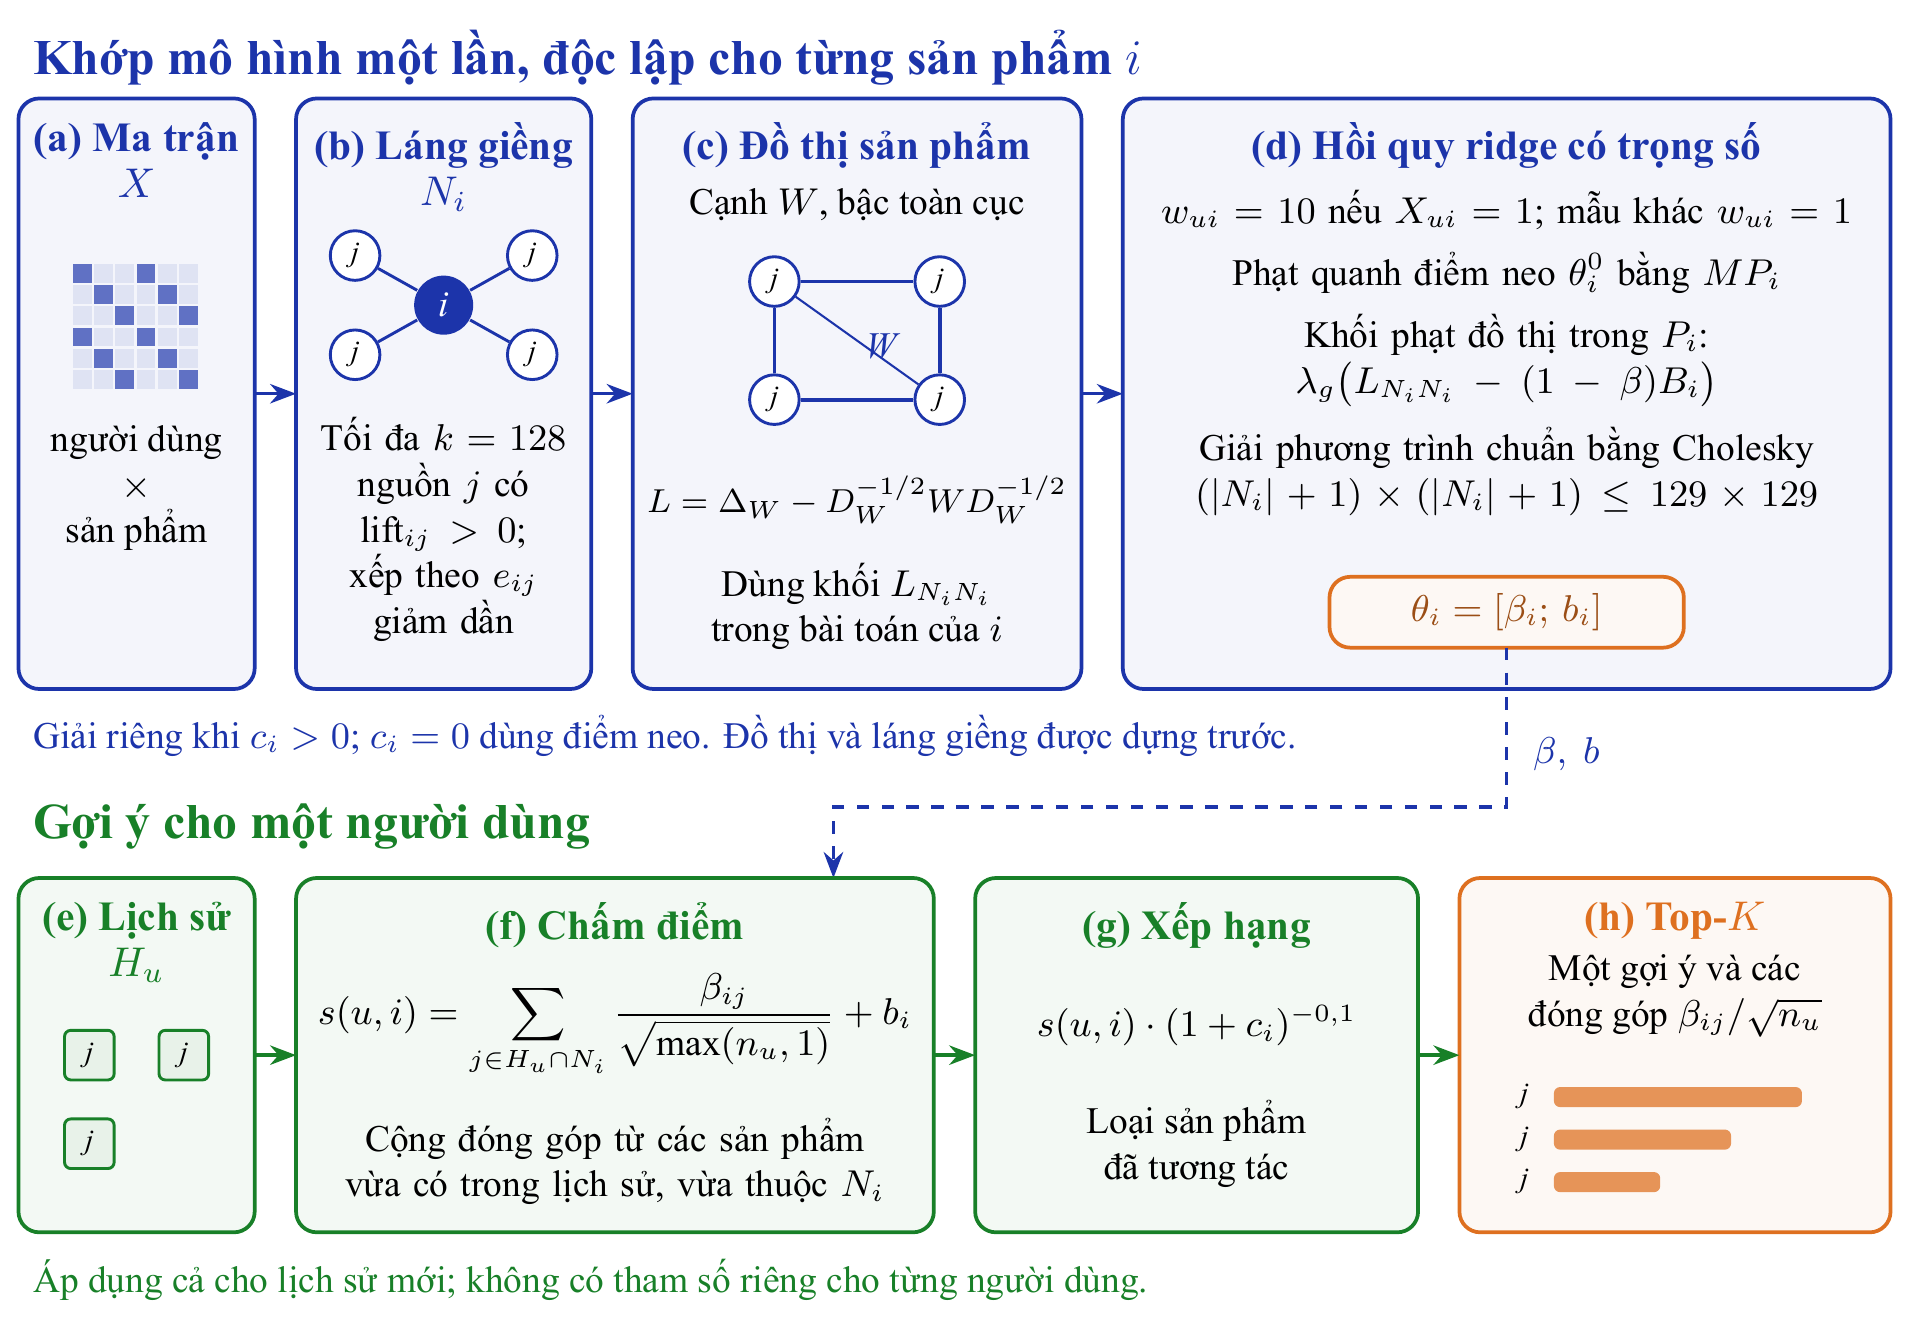
\includegraphics[width=\linewidth]{grnr_diagram.png}
\caption{Sơ đồ hoạt động của GRNR}
\label{fig:grnr-diagram}
\end{figure}

Đồ thị sản phẩm được dựng một lần trên toàn danh mục, và mỗi bài toán hồi quy lấy khối ứng với tập nguồn của nó. Sau khi giải, hệ số và hệ số chặn được giữ cố định; khi có lịch sử mới, mô hình tính điểm, điều chỉnh theo độ phổ biến rồi chọn top-$K$.


\subsubsection{Lựa chọn láng giềng và đồ thị sản phẩm}
\label{sec:grnr-neighbors}

GRNR làm việc với ma trận đồng xuất hiện đã xóa đường chéo $C^\circ$ theo Định nghĩa~\ref{def:cooccurrence}. Với sản phẩm đích $i$, xác suất nền đã làm trơn là
\begin{equation}
p_i = \frac{c_i+1}{|\mathcal{U}|+2}.
\end{equation}
Với mỗi sản phẩm nguồn $j\ne i$, mức đồng xuất hiện vượt kỳ vọng và điểm dư đã làm trơn là
\begin{equation}
e_{ij} = C^\circ_{ji} - c_j\,p_i, \qquad \mathrm{lift}_{ij} = \frac{e_{ij}}{c_j+\kappa_{\mathrm{lift}}}, \quad \kappa_{\mathrm{lift}} = 10.
\label{eq:grnr-lift}
\end{equation}
Điểm dư $\mathrm{lift}_{ij}$ này khác với tỉ số lift ở Mục~\ref{sec:cooccurrence}. Với mỗi đích, nhóm chọn tối đa $k=128$ nguồn có điểm dương, xếp theo $e_{ij}$ giảm dần, và theo chỉ số sản phẩm khi bằng điểm. Phép trừ $c_jp_i$ loại phần đồng xuất hiện chỉ do độ phổ biến mà có, còn việc xếp theo $e_{ij}$ ưu tiên những nguồn vượt kỳ vọng nhiều nhất về số lượng tuyệt đối. Cosin hay tỉ số lift chuẩn hóa đồng xuất hiện theo cách khác nên có thể chọn ra các nguồn khác. Vì $c_j+\kappa_{\mathrm{lift}}>0$, tham số $\kappa_{\mathrm{lift}}$ chỉ ảnh hưởng đến trọng số đồ thị, không làm đổi dấu hay thứ tự chọn nguồn.

Các trọng số lift dương tạo thành một đồ thị sản phẩm có hướng, $W^{\mathrm{dir}}_{ij}=\mathrm{lift}_{ij}$ với $j\in N_i$. Đồ thị được đối xứng hóa bằng $W=\max(W^{\mathrm{dir}}, W^{\mathrm{dir}\top})$, rồi lấy Laplacian chuẩn hóa
\begin{equation}
L = \Delta_W - D_W^{-1/2}\, W\, D_W^{-1/2},
\end{equation}
trong đó $W$ đóng vai trò ma trận kề $A$ ở Định nghĩa~\ref{def:laplacian}, $D_W$ là ma trận bậc, và $\Delta_W$ có đường chéo bằng 1 ở đỉnh có bậc dương, bằng 0 ở đỉnh cô lập; nghịch đảo căn bậc tại đỉnh cô lập được quy ước bằng 0. Phép lấy max giữ một cạnh nếu ít nhất một trong hai hướng được chọn, với trọng số lớn hơn của hai hướng; lấy trung bình cũng là một lựa chọn hợp lệ nhưng cho mức phạt khác.

Dùng Laplacian chuẩn hóa nghĩa là nhóm phạt chênh lệch giữa các hệ số đã chia cho căn bậc trên những cạnh mạnh. Đại lượng này khác với chênh lệch hệ số thô trong Laplacian không chuẩn hóa, và khác với phạt ridge, vốn co từng hệ số về điểm neo một cách độc lập~\cite[Mục~1.2, 1.4]{chung1997spectral}.

\subsubsection{Hàm mục tiêu và phương pháp giải}
\label{sec:grnr-objective}

Với sản phẩm $i$, mỗi người dùng $u$ được mô tả bởi vector đặc trưng gồm các láng giềng có trong lịch sử, chuẩn hóa theo độ dài lịch sử, và một hệ số chặn:
\begin{equation}
\phi_u^{(i)} = \left[\, \frac{X_{u,N_i}}{\sqrt{\max(n_u - X_{ui},\,1)}} \;;\; 1 \,\right] \in \mathbb{R}^{|N_i|+1}.
\label{eq:grnr-feature}
\end{equation}
Mẫu số dùng $n_u-X_{ui}$ để không tính chính sản phẩm đích vào độ dài lịch sử khi tạo mẫu dương, cho khớp với lúc dự đoán một sản phẩm chưa thấy. Chuẩn hóa theo căn độ dài làm giảm đóng góp của lịch sử dài so với tổng thô, nhưng giảm ít hơn phép lấy trung bình, như phân tích ở Mục~\ref{sec:dfhf-representation}. Với $c_i>0$, tham số $\theta_i=[\beta_i;b_i]$ được ước lượng bằng bình phương tối thiểu có trọng số:
\begin{equation}
\min_{\theta_i}\; \frac12\sum_{u\in\mathcal{U}} w_{ui}\bigl(X_{ui} - \phi_u^{(i)\top}\theta_i\bigr)^2 \;+\; \frac12(\theta_i-\theta_i^0)^\top M P_i\,(\theta_i-\theta_i^0),
\label{eq:grnr-objective}
\end{equation}
với $w_{ui}=\omega_+=10$ nếu $X_{ui}=1$, $w_{ui}=1$ trong trường hợp còn lại, và $M=|\mathcal{U}|$. Trọng số 10 cho mẫu dương thể hiện rằng tương tác đã quan sát đáng tin hơn ô chưa quan sát, theo hướng của Hu và cộng sự~\cite{hu2008wmf}. Nhân phạt với $M$ tương đương với chia phần sai số dữ liệu cho số người dùng và giữ nguyên ma trận phạt $P_i$.

Khi tập láng giềng đã cố định, hàm mục tiêu là bậc hai theo $\theta_i$, nên nghiệm có được bằng cách giải một hệ tuyến tính. Hồi quy logistic hợp với nhãn nhị phân hơn nhưng thường cần tối ưu lặp; thêm phạt $L_1$ có thể làm hệ số thưa trong tập nguồn nhưng cũng làm mất dạng một hệ Cholesky~\cite[Mục~6.1, 6.3]{boyd2004convex}. Nhóm chọn cấu trúc bậc hai để giải trực tiếp; điểm dự đoán chỉ dùng để xếp hạng nên không cần nằm trong $[0,1]$. Ma trận phạt là
\begin{equation}
P_i = \begin{bmatrix} \eta\,\mathrm{diag}(s_j)_{j\in N_i} + \lambda_g\bigl(L_{N_iN_i} - (1-\beta)B_i\bigr) & 0 \\ 0 & \eta_b \end{bmatrix},
\label{eq:grnr-precision}
\end{equation}
trong đó $\eta=10^{-5}$, $\eta_b=10^{-3}$, $\lambda_g=10^{-3}$ và $\beta=0{,}5$; ở đây $\beta$ là hệ số biên vô hướng, khác vector hồi quy $\beta_i$. Hệ số phạt riêng của từng nguồn là $s_j=\min\bigl((c_j/(c_j+\alpha_s))^{-2},s_{\max}\bigr)$, với $\alpha_s=2$ và $s_{\max}=10$. Khi $c_j$ tăng, $s_j$ giảm dần về 1, nghĩa là nguồn càng ít dữ liệu càng bị co mạnh; số mũ 2 quy định tốc độ giảm. Vì $c_j\ge1$ nên $s_j\le9$, và ngưỡng 10 không có tác dụng trong cấu hình này.

$L_{N_iN_i}$ là khối con của Laplacian toàn cục ứng với tập nguồn, còn $B_i\in\mathbb{R}^{|N_i|\times|N_i|}$ là ma trận đường chéo chứa phần năng lượng của các liên kết ra ngoài $N_i$. Hệ số $\beta$ nội suy giữa việc bỏ hẳn phần biên khi $\beta=0$ và giữ đủ khi $\beta=1$; giá trị $0{,}5$ giữ một nửa và chưa được chứng minh là tối ưu. Điểm neo $\theta_i^0$ có các hệ số láng giềng bằng 0 và hệ số chặn đặt theo xác suất nền đã làm trơn:
\begin{equation}
b_i^0 = \frac{\omega_+\,p_i}{1+(\omega_+-1)\,p_i}, \quad \omega_+=10.
\end{equation}

Nếu chỉ khớp một hằng số với dữ liệu gốc dưới trọng số $\omega_+$, nghiệm của phần sai số là $\omega_+c_i/(M+(\omega_+-1)c_i)$. Thay $c_i/M$ bằng $p_i$ đã làm trơn cho ra điểm neo trên; với $0<p_i<1$, điểm neo thỏa $b_i^0/(1-b_i^0)=\omega_+p_i/(1-p_i)$. Như vậy hệ số chặn được kéo về xác suất nền đã điều chỉnh theo trọng số, thay vì về 0.

Để áp dụng kết quả về nghiệm duy nhất ở Mục~\ref{sec:ridge}, cần kiểm tra $P_i$ xác định dương. Gọi $\delta_j=\sum_kW_{jk}$ là bậc toàn cục. Với $j\in N_i$, phần tử đường chéo của $B_i$ là $\sum_{k\notin N_i}W_{jk}/\delta_j$ nếu $\delta_j>0$, và bằng 0 nếu $\delta_j=0$. Với vector hệ số $z$ trên $N_i$, đặt $a_j=z_j/\sqrt{\delta_j}$ khi bậc dương, bằng 0 trong trường hợp còn lại. Từ công thức năng lượng~\eqref{eq:laplacian-quadratic},
\begin{equation}
\begin{aligned}
z^\top\bigl(L_{N_iN_i}-(1-\beta)B_i\bigr)z
={}&\frac12\sum_{j,k\in N_i}W_{jk}(a_j-a_k)^2\\
&+\beta\sum_{j\in N_i}(B_i)_{jj}z_j^2\ge0.
\end{aligned}
\label{eq:grnr-penalty-energy}
\end{equation}
Bất đẳng thức đúng với $\beta\in[0,1]$. Vì $\eta>0$, $s_j>0$, $\eta_b>0$ và $\lambda_g\ge0$, hai khối của $P_i$ đều xác định dương; nếu không có láng giềng, chỉ còn khối chặn $\eta_b$. Như vậy $P_i\succ0$. Áp dụng kết quả ở Mục~\ref{sec:ridge} với ma trận phạt $MP_i$ và điểm neo $\theta_i^0$, bài toán có nghiệm duy nhất thỏa
\begin{equation}
\bigl(\Phi_i^\top \Omega_i \Phi_i + M P_i\bigr)\,\theta_i = \Phi_i^\top \Omega_i\, x_i + M P_i\,\theta_i^0,
\label{eq:grnr-normal}
\end{equation}
với $\Phi_i$ là ma trận xếp các hàng $\phi_u^{(i)}$, $\Omega_i=\mathrm{diag}(w_{ui})$ và $x_i$ là cột $i$ của $X$. Hệ~\eqref{eq:grnr-normal} có kích thước tối đa $129\times129$ và được giải bằng Cholesky ở độ chính xác số thực 64 bit. Cài đặt kiểm tra sai số dư tương đối $\|G_i\theta_i-r_i\|/\max(\|r_i\|,10^{-15})<10^{-8}$ cho từng sản phẩm có tương tác, với $G_i,r_i$ là ma trận và vế phải của hệ.

Với $c_i=0$, GRNR không giải hồi quy mà dùng luôn điểm neo, $\theta_i\leftarrow\theta_i^0$. Các sản phẩm này không thuộc tập ứng viên $\mathcal{I}_+$, nên quy tắc dự phòng này không ảnh hưởng đến đánh giá.

\subsubsection{Thuật toán huấn luyện và suy luận}
\label{sec:grnr-algorithm}

Ma trận Gram $\Phi_i^\top\Omega_i\Phi_i$ của mỗi bài toán được lấy từ một ma trận dùng chung rồi hiệu chỉnh ở các mẫu dương. Phần lớn người dùng có $X_{ui}=0$ và trọng số 1, nên đóng góp của họ có sẵn trong Gram toàn cục $G=\tilde X^\top\tilde X$ của lịch sử chuẩn hóa $\tilde X_{uj}=X_{uj}/\sqrt{\max(n_u,1)}$. Với người dùng có $X_{ui}=1$, nhóm thay đúng hàng đặc trưng đã loại $i$ khỏi mẫu số và gán trọng số 10, như ở Thuật toán~\ref{alg:grnr}.

\begin{algorithm}[H]
\caption{Huấn luyện và chấm điểm GRNR}
\label{alg:grnr}
\KwIn{Ma trận tương tác giữ lại $X$; siêu tham số ở \tabref{tab:grnr-hparams}}
\KwOut{Ma trận hệ số thưa $\mathcal{B}\in\mathbb{R}^{|\mathcal{I}|\times|\mathcal{I}|}$, vector chặn $b$}
Tính $c$, $p$, $n$; kiểm tra cận $H=\sum_u n_u^2\le5\cdot10^7$\;
Tính đồng xuất hiện $C=X^\top X$ và xóa đường chéo\;
\ForEach{sản phẩm $i$}{
  Chọn $N_i$ theo \eqref{eq:grnr-lift}; ghi trọng số vào $W^{\mathrm{dir}}$\;
}
Đối xứng hóa $W=\max(W^{\mathrm{dir}},W^{\mathrm{dir}\top})$; tính Laplacian $L$\;
Tính lịch sử chuẩn hóa $\tilde X$ và Gram toàn cục $G=\tilde X^\top\tilde X$\;
\ForEach{sản phẩm $i$}{
  \eIf{$c_i=0$}{$\theta_i\leftarrow\theta_i^0$\;}{
  Lấy khối Gram của $N_i$ từ $G$, thay chính xác các hàng của người dùng có $X_{ui}=1$\;
  Lập $P_i$ theo \eqref{eq:grnr-precision}; giải \eqref{eq:grnr-normal} bằng Cholesky; kiểm tra sai số dư\;}
  Ghi $\beta_i$ vào cột $i$ của $\mathcal{B}$ và $b_i$ vào $b$\;
}
Chấm điểm: $s(u,i)=\tilde X_{u,:}\,\mathcal{B}_{:,i}+b_i$; khi xếp hạng dùng $s(u,i)\cdot(1+c_i)^{-0{,}1}$\;
\end{algorithm}

Với quy ước $\mathcal{B}_{ji}=\beta_{ij}$ khi $j\in N_i$ và bằng 0 ngoài tập nguồn, điểm của người dùng $u$ cho sản phẩm $i$ khi suy luận là
\begin{equation}
s(u,i)=\sum_{j\in H_u\cap N_i}\beta_{ij}/\sqrt{\max(n_u,1)}+b_i.
\end{equation}
Khi xếp hạng, điểm được nhân với $(1+c_i)^{\rho_{\mathrm{pop}}}$, với $\rho_{\mathrm{pop}}=-0{,}1$. Hàm lũy thừa điều chỉnh liên tục theo số đếm, và việc cộng 1 giữ biểu thức xác định tại $c_i=0$. Với điểm dương, phép nhân hạ điểm của sản phẩm phổ biến nhiều hơn; với điểm âm, tác động có thể ngược chiều. Bước điều chỉnh diễn ra sau hồi quy nên không tham gia~\eqref{eq:grnr-objective}. Khi lịch sử rỗng, điểm chỉ còn hệ số chặn trước khi điều chỉnh.

Vì điểm là một tổng tuyến tính, có thể tách riêng đóng góp $\beta_{ij}/\sqrt{n_u}$ của từng sản phẩm $j$ trong lịch sử. Phân rã này giải thích điểm số bằng các thành phần đại số, không cho biết vì sao người dùng thích sản phẩm.


\subsection{Diffusion-Filtered History Factorization}
\label{sec:dfhf}

Để trả lời câu hỏi ở Mục~\ref{sec:trained-gap}, DFHF xây biểu diễn người dùng từ lịch sử bằng cách kết hợp hai bảng embedding nguồn và đích với bộ lọc khuếch tán và hàm mất mát softmax. Mô hình kế thừa cách tổng hợp lịch sử của Factored Item Similarity Models (FISM)~\cite{kabbur2013fism} và biểu diễn bất đối xứng của Koren~\cite{koren2008factorization}; bộ lọc đa thức theo nguyên tắc tránh phân rã phổ của Turbo-CF~\cite{park2024turbocf}, còn việc cho các sản phẩm cạnh tranh xác suất trên toàn danh mục có tiền lệ ở Multinomial Variational Autoencoder (Mult-VAE)~\cite{liang2018multvae}. Điểm riêng của DFHF là lọc cả hai bảng sản phẩm, học từ ngữ cảnh đã bỏ sản phẩm đích, và có quy tắc riêng cho lịch sử chỉ gồm một sản phẩm. \Figref{fig:dfhf-diagram} tóm tắt quy trình: hàng trên là vòng huấn luyện, hàng dưới là bước gợi ý từ lịch sử. Vì lịch sử đơn có trọng số bằng 0, người dùng chỉ có một tương tác được chấm điểm bằng hệ số chặn $b$.

\begin{figure}[H]
\centering
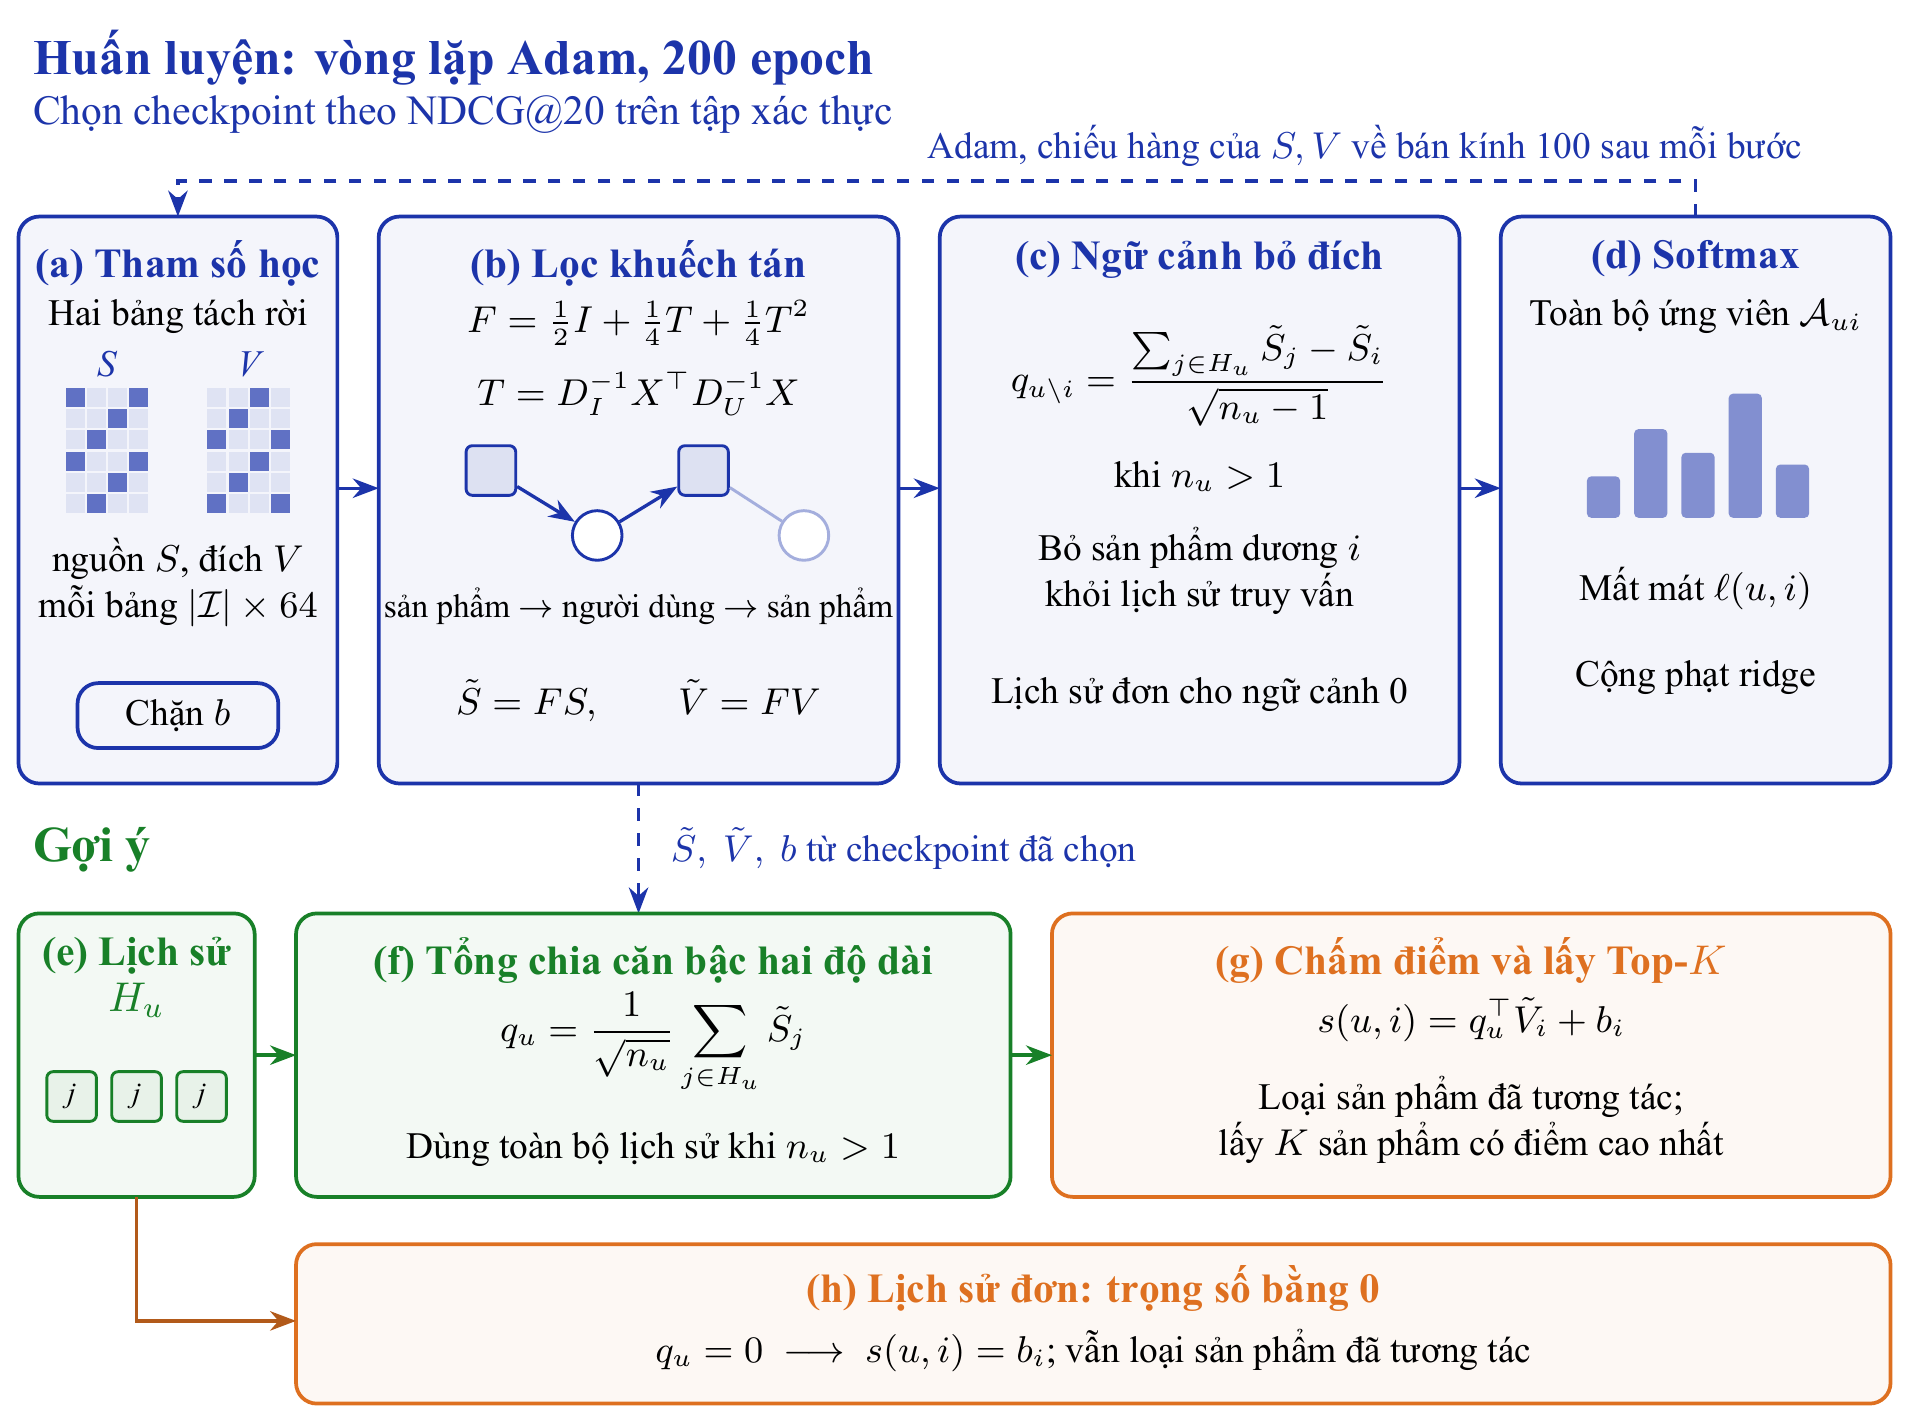
\includegraphics[width=\linewidth]{dfhf_diagram.png}
\caption{Sơ đồ hoạt động của DFHF}
\label{fig:dfhf-diagram}
\end{figure}

Trong vòng huấn luyện, mỗi lô tính lại hai bảng đã lọc rồi cập nhật tham số từ ngữ cảnh đã bỏ đích. Khi gợi ý, các bảng lấy từ checkpoint, tức bản lưu tham số tại một epoch, được giữ cố định và lịch sử được tổng hợp theo~\eqref{eq:dfhf-score}. Nhờ các bảng sản phẩm cố định, biểu diễn được tính lại ngay khi lịch sử thay đổi mà không cần vector tham số riêng cho người dùng. Cấu hình cụ thể ở \tabref{tab:dfhf-hparams}.


\subsubsection{Biểu diễn lịch sử và bộ lọc khuếch tán}
\label{sec:dfhf-representation}

DFHF có hai bảng sản phẩm, mỗi bảng $f=64$ chiều: bảng nguồn $S\in\mathbb{R}^{|\mathcal{I}|\times f}$ mô tả sản phẩm khi nằm trong lịch sử, bảng đích $V\in\mathbb{R}^{|\mathcal{I}|\times f}$ mô tả sản phẩm khi được chấm điểm, cùng vector chặn $b\in\mathbb{R}^{|\mathcal{I}|}$. Hai bảng độc lập cho phép quan hệ không đối xứng, tức $\tilde S_j^\top\tilde V_i$ có thể khác $\tilde S_i^\top\tilde V_j$; nếu buộc $S=V$, thành phần sản phẩm--sản phẩm sẽ là một ma trận Gram đối xứng. Sự linh hoạt này phải trả bằng một bảng tham số thứ hai, theo hướng nhân tố hóa của FISM~\cite{kabbur2013fism}.

Toán tử $T$ ở~\eqref{eq:transition} lấy trung bình qua hai bước sản phẩm--người dùng--sản phẩm. Nhờ chia cho bậc, mỗi hàng của $T$ có tổng bằng 1, khác với đồng xuất hiện thô vốn còn mang quy mô số đếm. Bộ lọc là
\begin{equation}
F = \tfrac12 I + \tfrac14 T + \tfrac14 T^2
\label{eq:dfhf-filter}
\end{equation}
và được áp cho cả hai bảng: $\tilde S=FS$, $\tilde V=FV$. Thành phần $I$ giữ lại một nửa vector gốc, còn $T$ và $T^2$ thêm hai mức lan truyền giữa các sản phẩm; dừng ở bậc hai giới hạn chi phí ở hai lần áp $T$ cho mỗi bảng. Vì các hệ số không âm và có tổng bằng 1, $F$ vẫn là một phép lấy trung bình và không làm tăng giá trị lớn nhất theo từng chiều, theo Nhận xét~\ref{rem:transition-filter}. Sản phẩm cô lập giữ nguyên vector gốc. So với $F=I$, bộ lọc đưa thông tin đồng tương tác vào tham số hóa; so với $\tfrac12I+\tfrac12T$, nó thêm một mức lan truyền với giá thêm một lần áp $T$. Các tính chất này giải thích hành vi và chi phí của bộ lọc, nhưng chưa xác nhận bộ hệ số $(1/2,1/4,1/4)$ tốt hơn các lựa chọn khác.

Gọi $\zeta_{\mathrm{hist}}=0{,}5$ là số mũ chuẩn hóa lịch sử và $\omega_1=0$ là trọng số của lịch sử đơn. Số mũ 0 ứng với tổng thô, số mũ 1 ứng với trung bình, và căn độ dài nằm giữa hai cách này. FISM khảo sát số mũ trong $[0,1]$ và báo cáo kết quả tốt quanh $0{,}4$--$0{,}5$~\cite[Mục~4, 7.2]{kabbur2013fism}; đây là tiền lệ để chọn $0{,}5$ chứ không chứng minh giá trị này tối ưu cho DFHF. Chia cho căn độ dài chỉ ổn định phương sai khi các vector thỏa một số giả thiết về tương quan, mà các vector đã học không nhất thiết thỏa. Với các giá trị đang dùng,
\begin{equation}
q_u=\begin{cases}
\displaystyle \frac{1}{n_u^{\zeta_{\mathrm{hist}}}}\sum_{j\in H_u}\tilde S_j,&n_u\ge2,\\
0,&n_u\le1,
\end{cases}
\qquad s(u,i)=q_u^\top\tilde V_i+b_i.
\label{eq:dfhf-score}
\end{equation}
Khi $n_u\le1$, điểm chỉ còn $b_i$, dù danh sách cuối vẫn có thể khác nhau vì lịch sử đã được loại khỏi ứng viên. Với $n_u=0$, không có gì để tổng hợp. Với $n_u=1$, đặt $\omega_1=0$ là chủ động bỏ thông tin của sản phẩm duy nhất; giữ trọng số khác 0 cũng là một phương án. Đây là một lựa chọn thiết kế, không phải hệ quả bắt buộc của việc không dùng vector người dùng.

Với giá trị riêng $\lambda_T\in[0,1]$ của $T$, đáp ứng của bộ lọc $h(\lambda_T)=\tfrac12+\tfrac14\lambda_T+\tfrac14\lambda_T^2$ thuộc $[1/2,1]$, nên $F$ khả nghịch. Nếu bỏ qua phạt và giới hạn chuẩn, hai bảng tự do $S,V$ vẫn biểu diễn được mọi cặp $\tilde S,\tilde V$ qua phép đổi biến này. Bộ lọc vì thế tác động qua tham số hóa, điều chuẩn và quá trình tối ưu, chứ không áp một ràng buộc cứng buộc nghiệm phải trơn.

\subsubsection{Hàm mục tiêu và phương pháp tối ưu}
\label{sec:dfhf-objective}

Mỗi truy vấn huấn luyện $(u,i)$ được lấy qua hai bước: chọn đều một người dùng $u\in\mathcal{U}_+$, rồi chọn đều một sản phẩm $i\in H_u$. Xác suất lấy một truy vấn cụ thể là $1/(|\mathcal{U}_+|n_u)$, nên các cạnh không được lấy đều nhau khi độ dài lịch sử khác nhau. Với $n_u>1$, ngữ cảnh huấn luyện bỏ chính sản phẩm dương ra khỏi lịch sử:
\begin{equation}
q_{u\setminus i} = \frac{1}{(n_u-1)^{\zeta_{\mathrm{hist}}}}\Bigl(\sum_{j\in H_u}\tilde S_j - \tilde S_i\Bigr).
\end{equation}
Với $n_u=1$, ngữ cảnh bằng 0 vì bỏ sản phẩm dương thì lịch sử rỗng. Khi $n_u=2$, ngữ cảnh vẫn tổng hợp sản phẩm còn lại theo công thức trên, vì quy tắc lịch sử đơn căn cứ vào độ dài lịch sử $n_u$ chứ không phải độ dài sau khi bỏ đích. Tập so sánh khi học là $\mathcal{A}_{ui}=(\mathcal{I}_+\setminus H_u)\cup\{i\}$: tập này giữ đích dương, loại các tương tác khác của người dùng và các sản phẩm cô lập. Hàm mất mát entropy chéo là
\begin{equation}
\ell(u,i) = -\log\frac{\exp\bigl((q_{u\setminus i}^\top\tilde V_i + b_i)/\tau_{\mathrm{sm}}\bigr)}{\sum_{i'\in\mathcal{A}_{ui}}\exp\bigl((q_{u\setminus i}^\top\tilde V_{i'} + b_{i'})/\tau_{\mathrm{sm}}\bigr)},
\label{eq:dfhf-loss}
\end{equation}
với nhiệt độ $\tau_{\mathrm{sm}}=1$. Softmax đặt mọi ứng viên vào cùng một mẫu số, nên tăng điểm của một sản phẩm khác đích sẽ làm giảm xác suất của đích. Entropy chéo nhị phân thì xét riêng từng nhãn, còn Bayesian Personalized Ranking (BPR) so từng cặp dương--âm. Tính đủ mẫu số giúp tránh lấy mẫu một tập âm nhỏ như softmax lấy mẫu, đổi lại phải tính điểm trên toàn danh mục. Mult-VAE là tiền lệ cho kiểu cạnh tranh xác suất đa thức này~\cite{liang2018multvae}, nhưng DFHF dùng ngữ cảnh xác định và tập ứng viên đã loại lịch sử, nên kết quả của bài đó không trở thành bảo đảm cho hàm mất mát ở đây.

Tập $\mathcal{A}_{ui}$ được xác định từ dữ liệu huấn luyện, còn tập ứng viên khi đánh giá tuân theo Mục~\ref{sec:evaluation-unit}.

Gọi $\pi_i$ là xác suất sản phẩm $i$ được chọn làm đích dưới quy tắc lấy mẫu trên. Khi đó,
\begin{equation}
\pi_i=\frac{1}{|\mathcal{U}_+|}\sum_{u\in\mathcal{U}_+}\frac{X_{ui}}{n_u},
\qquad \sum_{i\in\mathcal{I}}\pi_i=1.
\label{eq:dfhf-exposure}
\end{equation}
Mục tiêu kỳ vọng theo phân phối truy vấn, cộng phạt trên hai bảng tham số gốc và vector chặn, là
\begin{equation}
\begin{aligned}
\mathcal{L}={}&\frac{1}{|\mathcal{U}_+|}\sum_{u\in\mathcal{U}_+}\frac{1}{n_u}\sum_{i\in H_u}\ell(u,i)\\
&+\frac{\lambda_{\mathrm{emb}}}{2}\sum_i\pi_i\frac{\|V_i\|^2+\|S_i\|^2}{2}
+\frac{\lambda_b}{2}\|b\|^2,
\end{aligned}
\label{eq:dfhf-objective}
\end{equation}
với $\lambda_{\mathrm{emb}}=0{,}1$ và $\lambda_b=10^{-4}$. Trung bình hàm mất mát trên lô ước lượng thành phần xếp hạng. Trọng số $\pi_i$ làm cho phạt bằng kỳ vọng mức phạt tại sản phẩm được lấy làm đích, thay vì phạt đều mọi hàng. Nhóm dùng cùng $\pi_i$ cho cả $S$ và $V$, dù tần suất một sản phẩm xuất hiện trong lịch sử nguồn có thể khác $\pi_i$; cả hai số hạng phạt được tính trên toàn bảng ở mỗi bước.

Tham số được cập nhật bằng Adaptive Moment Estimation (Adam), thuật toán điều chỉnh bước cập nhật theo các mômen của gradient~\cite{kingma2015adam}. Sau mỗi bước Adam, gọi $z\in\mathbb{R}^f$ là một hàng vừa cập nhật của $S$ hoặc $V$, và $\hat v_{t,i}$ là mômen bậc hai đã hiệu chỉnh sai lệch của hàng đó tại bước $t$. Với $\epsilon=10^{-8}$, ma trận khoảng cách đường chéo là $D_{t,i}^{\mathrm{Adam}}=\mathrm{diag}(\sqrt{\hat v_{t,i}}+\epsilon)$, với căn và phép cộng tính theo từng tọa độ. Phép chiếu được định nghĩa bởi
\begin{equation}
\Pi_{R}^{D}(z)=\underset{\|x\|_2\le R}{\arg\min}\;
\frac12(x-z)^\top D(x-z),\qquad R=R_{\mathrm{emb}}=100.
\label{eq:dfhf-metric-projection}
\end{equation}
Nếu $z$ nằm trong cầu thì giữ nguyên; nếu nằm ngoài, nghiệm có tọa độ $x_k=D_{kk}z_k/(D_{kk}+\mu)$, với $\mu>0$ tìm bằng chia đôi sao cho $\|x\|_2=R$. Vì $D$ thường không tỉ lệ với $I$, phép chiếu này khác với việc co vector về tâm theo khoảng cách Euclid. Giới hạn chuẩn khống chế độ lớn của từng hàng tham số, còn phạt ridge vẫn hoạt động bên trong miền đó. Vector chặn chỉ chịu phạt $\lambda_b$, không bị chiếu. Bán kính 100 là giá trị được dùng, chưa được xác nhận tối ưu bằng phân tích độ nhạy.

\subsubsection{Thuật toán huấn luyện và suy luận}
\label{sec:dfhf-algorithm}

DFHF được huấn luyện bằng Adam với tốc độ học $\mathrm{lr}=0{,}0003$, hai hệ số mômen $\beta_{1,\mathrm{Adam}}=0{,}9$, $\beta_{2,\mathrm{Adam}}=0{,}999$, lô tối đa $Q_{\mathrm{batch}}=2048$ truy vấn và $N_{\mathrm{ep}}=200$ epoch. Mỗi epoch lấy độc lập $|E|$ truy vấn theo quy tắc chọn người dùng rồi chọn sản phẩm, nên một cạnh có thể được lấy nhiều lần hoặc không được lấy. Thuật toán~\ref{alg:dfhf} tóm tắt toàn bộ vòng huấn luyện.

\begingroup
\setlength{\intextsep}{6pt}
\SetAlgoSkip{smallskip}
\begin{algorithm}[H]
\caption{Huấn luyện DFHF}
\label{alg:dfhf}
\KwIn{Tập cạnh giữ lại $E$; siêu tham số ở \tabref{tab:dfhf-hparams}}
\KwOut{Checkpoint $(S,V,b)$ có NDCG@20 tập xác thực cao nhất}
Khởi tạo $V\sim\mathcal{N}(0,1/f)$, $S\leftarrow V$ (sau đó cập nhật độc lập), $b\leftarrow0$\;
\For{epoch $=1,\dots,N_{\mathrm{ep}}$}{
  Lấy một dãy $|E|$ truy vấn độc lập: $u\sim\mathrm{Unif}(\mathcal{U}_+)$, rồi $i\sim\mathrm{Unif}(H_u)$\;
  Chia dãy thành các lô tối đa $Q_{\mathrm{batch}}$ truy vấn, cho phép truy vấn lặp\;
  \ForEach{lô truy vấn trong dãy}{
    Tính $\tilde S=FS$, $\tilde V=FV$ theo \eqref{eq:dfhf-filter}\;
    Tính ngữ cảnh $q_{u\setminus i}$ và hàm mất mát \eqref{eq:dfhf-loss} cộng phạt\;
    Cập nhật Adam với $\mathrm{lr}$; chiếu hàng của $S,V$ về bán kính $R_{\mathrm{emb}}$ theo khoảng cách của Adam\;
  }
  Đánh giá NDCG@20 trên tập xác thực; lưu checkpoint nếu tốt hơn\;
}
\end{algorithm}

Khi suy luận, các bảng sản phẩm từ checkpoint được giữ cố định và lịch sử được tổng hợp theo~\eqref{eq:dfhf-score}, với quy tắc riêng cho lịch sử rỗng và lịch sử đơn. Cách chọn checkpoint và siêu tham số được trình bày ở Mục~\ref{sec:protocol}.

\endgroup

\subsection{Phân tích tính chất và chi phí tính toán}
\label{sec:complexity}

\Tabref{tab:complexity} so sánh GRNR với EASE: GRNR lưu tối đa $(k+1)|\mathcal{I}|$ hệ số kể cả hệ số chặn, còn EASE đầy đủ có $|\mathcal{I}|(|\mathcal{I}|-1)$ hệ số ngoài đường chéo. \Tabref{tab:complexity-trained} so sánh DFHF với Light Graph Convolution Network (LightGCN): DFHF chỉ lưu bảng sản phẩm, còn LightGCN có thêm bảng người dùng. Với $k=128$ và $f=64$, GRNR có tối đa $129|\mathcal{I}|$ hệ số, còn DFHF học đúng $129|\mathcal{I}|$ tham số.

\begin{table}[H]
\centering
\small
\begin{tabularx}{\textwidth}{@{}p{3cm}>{\raggedright\arraybackslash}X>{\raggedright\arraybackslash}X@{}}
\toprule
 & GRNR & EASE đầy đủ \\
\midrule
Vector tham số người dùng & Không & Không \\
Số hệ số và chặn & $\le(k+1)|\mathcal{I}|$ & $|\mathcal{I}|(|\mathcal{I}|-1)$ hệ số ngoài đường chéo \\
Cách xác định hệ số & Các hệ tuyến tính kích thước tối đa $(k+1)\times(k+1)$ & Một phép nghịch đảo cỡ $|\mathcal{I}|\times|\mathcal{I}|$ \\
Khi lịch sử thay đổi & Tính lại điểm với hệ số cố định & Tính lại điểm với hệ số cố định \\
\bottomrule
\end{tabularx}
\caption{Đặc điểm lý thuyết của GRNR và EASE}
\label{tab:complexity}
\end{table}

Với GRNR, phần giải các hệ tốn $O(|\mathcal{I}|(k+1)^3)$, nhưng đây chỉ là một phần của giai đoạn khớp mô hình. Ngoài ra còn các bước dựng đồng xuất hiện $C$ và Gram $G$, chọn láng giềng và hiệu chỉnh mẫu dương. Đặt $H=\sum_u n_u^2$; việc tạo $C$ và $G$ duyệt các cặp sản phẩm trong từng lịch sử nên tốn $O(H)$. Nếu hàng $i$ của $C^\circ$ có $t_i$ phần tử khác 0, việc xếp nguồn để chọn láng giềng tốn tối đa $O(\sum_i t_i\log\max(t_i,1))$, còn hiệu chỉnh Gram theo mẫu dương tốn $O(|E|(k+1)^2)$.

Cài đặt kiểm tra trước cận $H\le5\cdot10^7$ và dừng lại nếu vượt, trước khi tạo ma trận đồng xuất hiện. Đây là điều kiện để phép tính được thực hiện, không phải cắt ma trận xuống một số phần tử cố định. Bộ nhớ tạm khi tạo $C$ hoặc $G$ có thể lớn hơn phần hệ số cuối cùng, vốn được lưu thưa ở mức $O(k|\mathcal{I}|)$, chưa kể dữ liệu lịch sử và đồ thị.

EASE~\cite{steck2019ease} tốn $O(|\mathcal{I}|^3)$ cho phép nghịch đảo và $O(|\mathcal{I}|^2)$ bộ nhớ cho ma trận đầy đủ, dù đường chéo của nghiệm bằng 0. Khi suy luận, cả hai phương pháp đều nhân lịch sử với hệ số đã lưu; GRNR còn cộng hệ số chặn và điều chỉnh theo độ phổ biến. Chi phí phép nhân thưa của GRNR phụ thuộc số hệ số trên các hàng ứng với sản phẩm có trong lịch sử.

\begin{table}[H]
\centering
\small
\begin{tabularx}{\textwidth}{@{}p{3cm}>{\raggedright\arraybackslash}X>{\raggedright\arraybackslash}X@{}}
\toprule
 & DFHF & LightGCN \\
\midrule
Vector tham số người dùng & Không & Có \\
Số tham số được học & $(2f+1)|\mathcal{I}|$ & $f(|\mathcal{U}|+|\mathcal{I}|)$ \\
Mục tiêu học & Softmax trên ứng viên hợp lệ, cộng phạt & BPR có điều chuẩn \\
Khi lịch sử thay đổi & Tổng hợp lại lịch sử với bảng sản phẩm cố định, theo quy tắc lịch sử đơn & Phân biệt tính lại lan truyền khi đổi đồ thị với cập nhật các vector tham số \\
\bottomrule
\end{tabularx}
\caption{Đặc điểm lý thuyết của DFHF và LightGCN}
\label{tab:complexity-trained}
\end{table}

Số tham số học của DFHF không phụ thuộc số người dùng, còn LightGCN~\cite{he2020lightgcn} có một vector riêng cho mỗi người dùng. Tuy vậy, DFHF vẫn phải lưu lịch sử và các cấu trúc thưa, nên tổng bộ nhớ của cài đặt vẫn phụ thuộc $|E|$, $|\mathcal{U}|$ và $|\mathcal{I}|$.

Gọi $Q_{\mathrm{batch}}=2048$ là số truy vấn tối đa trong lô và $B_{\mathrm{ep}}=\lceil |E|/Q_{\mathrm{batch}}\rceil$ là số lô mỗi epoch. Mỗi lô tính lại hai bảng đã lọc, mỗi bảng cần hai lần áp $T$, tức bốn lần áp toán tử. Một lần áp $T$ gồm hai phép nhân thưa, tốn $O(|E|f)$, cộng phần chuẩn hóa và xử lý hàng ở mức $O((|\mathcal{U}|+|\mathcal{I}|)f)$. Tính điểm chưa chuẩn hóa cho mọi sản phẩm rồi loại các phần tử ngoài $\mathcal{A}_{ui}$ tốn $O(Q_{\mathrm{batch}}|\mathcal{I}|f)$ mỗi lô. Gộp các hạng chính, chi phí một epoch huấn luyện là
\begin{equation}
O\!\left(|E|\,|\mathcal{I}|\,f
+B_{\mathrm{ep}}(|E|+|\mathcal{U}|+|\mathcal{I}|)f\right),
\label{eq:dfhf-epoch-cost}
\end{equation}
trong đó phép lọc được lặp lại ở mọi lô chứ không chỉ một lần đầu epoch. Khi tham số đã cố định, các bảng chỉ cần lọc và lịch sử chỉ cần tổng hợp một lần trước khi chấm điểm. Với $N_{\mathrm{val}}$ người dùng cần chấm điểm, phần tính điểm đầy đủ tốn $O(N_{\mathrm{val}}|\mathcal{I}|f)$, chưa kể chi phí tạo bảng và biểu diễn. Khi phục vụ lịch sử mới, các bảng đã lọc được giữ nguyên để tính tổng lịch sử và điểm ứng viên.

\clearpage
\section{Thiết lập thực nghiệm}
\label{sec:experiments}

\subsection{Dữ liệu và tiền xử lý}
\label{sec:data}

Nhóm sử dụng danh mục Electronics của bộ Amazon product data do McAuley và cộng sự công bố~\cite{mcauley2015image,he2016ups}, gồm các đánh giá thuộc bản 5-core và thông tin mô tả sản phẩm (metadata). Bản 5-core yêu cầu mỗi người dùng và sản phẩm có ít nhất 5 đánh giá. Nhóm lấy mã người dùng, mã sản phẩm, số sao và thời điểm từ từng đánh giá, rồi quy ước đánh giá từ 4 sao trở lên là một phản hồi tích cực, tức $X_{ui}=1$ theo Định nghĩa~\ref{def:implicit}. Tương tác ở đây là tín hiệu sở thích suy ra từ đánh giá công khai, không phải lượt mua. Thông tin mô tả chỉ cung cấp tên, thương hiệu và danh mục cho demo, không tham gia xếp hạng.
Nhóm khử các đánh giá tích cực trùng cặp người dùng--sản phẩm bằng cách giữ đánh giá mới nhất, ưu tiên số sao cao hơn nếu cùng thời điểm; dữ liệu này không có cặp trùng. Sau khi bỏ đánh giá thấp, một số người dùng và sản phẩm không còn đủ 5 tương tác, nên nhóm áp lại K-core hai phía với ngưỡng 5: loại các nút dưới ngưỡng, tính lại bậc và lặp đến khi hội tụ sau 13 vòng. Các mã còn lại được ánh xạ sang chỉ số liên tục theo thứ tự mã gốc. \Figref{fig:pipeline} ghi số tương tác qua từng bước: lọc số sao loại 333.121 đánh giá, khử trùng không loại đánh giá nào và K-core loại thêm 283.327 tương tác.

\begin{figure}[H]
\centering
\begin{tikzpicture}[node distance=0.55cm and 0.5cm, every node/.style={font=\small}]
\node[chthreeblue, text width=3.1cm] (raw) {Đánh giá thô\\1.689.188};
\node[chthreeblue, text width=3.1cm, right=of raw] (pos) {Giữ số sao $\ge4$\\1.356.067};
\node[chthreeblue, text width=3.1cm, right=of pos] (core) {K-core $\ge5$ (13 vòng)\\1.072.740};
\node[chthreegreen, text width=3.1cm, below=of core] (split) {Chia theo thời gian\\80/10/10};
\node[chthreepurple, text width=3.1cm, left=of split.north west, anchor=north east] (sparse) {Giảm tập huấn luyện\\$d\in\{1;0{,}75;0{,}5;0{,}25\}$};
\node[chthreeorange, text width=3.1cm, left=of sparse.north west, anchor=north east] (models) {Huấn luyện\\$\downarrow$\\Chọn mô hình trên tập xác thực\\$\downarrow$\\Đánh giá cuối cùng trên tập kiểm tra};
\draw[chthreeflow] (raw) -- (pos);
\draw[chthreeflow] (pos) -- (core);
\draw[chthreeflow] (core) -- (split);
\draw[chthreeflow] (split.west) -- (split.west -| sparse.east);
\draw[chthreeflow] (sparse.west) -- (sparse.west -| models.east);
\end{tikzpicture}
\caption{Quy trình tiền xử lý dữ liệu}
\label{fig:pipeline}
\end{figure}

\Tabref{tab:data-stats} thống kê dữ liệu trước khi chia tập. Mật độ tương tác bằng 0,0192\%, và một nửa người dùng có không quá 6 tương tác. Nhóm tạo thêm các mức độ thưa bằng cách giảm số tương tác huấn luyện.

\begin{table}[H]
\centering
\begin{tabular}{@{}lr@{}}
\toprule
Thống kê & Giá trị \\
\midrule
Số người dùng & 124.895 \\
Số sản phẩm & 44.843 \\
Số tương tác & 1.072.740 \\
Mật độ & 0,0192\% \\
Số tương tác mỗi người dùng: trung bình / trung vị / lớn nhất & 8,59 / 6 / 354 \\
Số tương tác trung bình mỗi sản phẩm & 23,9 \\
\bottomrule
\end{tabular}
\caption{Thống kê dữ liệu sau tiền xử lý}
\label{tab:data-stats}
\end{table}

Dữ liệu sau tiền xử lý được chia theo thời gian. Lịch sử của mỗi người dùng được sắp theo thời điểm đánh giá; các tương tác cùng thời điểm được sắp theo một hàm băm có seed của cặp người dùng--sản phẩm, rồi theo mã sản phẩm. Từ những người dùng có ít nhất 3 tương tác, nhóm chọn ngẫu nhiên 107.274 người dùng với seed 42; sau bước K-core, mọi người dùng đều thỏa điều kiện này. Con số 107.274 bằng 10\% tổng số tương tác, để tập xác thực và tập kiểm tra mỗi tập chiếm đúng 10\% dữ liệu.

Với mỗi người dùng được chọn, tương tác cuối cùng thuộc tập kiểm tra, tương tác áp cuối thuộc tập xác thực, còn các tương tác trước đó thuộc tập huấn luyện. 17.621 người dùng còn lại chỉ có mặt trong tập huấn luyện, nên tỉ lệ 80/10/10 ở \tabref{tab:split} tính trên tổng số tương tác chứ không áp riêng cho từng người dùng. Cách chia này cho mỗi người dùng được chọn đúng một mục tiêu, nhờ đó chất lượng được đo và so sánh ghép cặp theo từng người dùng; một mốc thời gian chung sẽ để lại nhiều người dùng không có mục tiêu nào. Trong \tabref{tab:split}, sản phẩm mới là sản phẩm không có trong tập huấn luyện.

\begin{table}[H]
\centering
\begin{tabular}{@{}lrrr@{}}
\toprule
 & Huấn luyện & Xác thực & Kiểm tra \\
\midrule
Số tương tác & 858.192 & 107.274 & 107.274 \\
Tỉ lệ & 80\% & 10\% & 10\% \\
Mục tiêu thuộc sản phẩm mới & --- & 59 & 187 \\
\bottomrule
\end{tabular}
\caption{Kết quả chia tập theo thời gian}
\label{tab:split}
\end{table}

Ba tập có ba vai trò tách biệt. Tập huấn luyện dùng để học tham số. Tập xác thực dùng để chọn siêu tham số và checkpoint theo NDCG@20. Sau khi chọn xong, cấu hình và checkpoint của từng mô hình được giữ cố định và đánh giá một lần trên tập kiểm tra. Mọi kết quả chất lượng và kiểm định ở Chương~\ref{sec:results} đều tính trên tập kiểm tra; chỉ các đường học và phân tích chọn checkpoint dùng tập xác thực. Tập kiểm tra không tham gia vào việc huấn luyện hay chọn mô hình.

\label{sec:sparsity-protocol}

Để khảo sát ảnh hưởng của độ thưa, tập huấn luyện được giữ lại ở các tỉ lệ $d\in\{1;0{,}75;0{,}5;0{,}25\}$, còn tập xác thực và tập kiểm tra giữ nguyên. Ở đây $d$ là tỉ lệ số tương tác huấn luyện còn lại so với tập đầy đủ; vì số người dùng và sản phẩm không đổi, mật độ của ma trận tương tác giảm theo $d$. Bốn mức cách đều nhau 25\%, đi từ tập đầy đủ đến mức mà phần lớn người dùng chỉ còn một tương tác, như \tabref{tab:sparsity} cho thấy.

Thuật toán giảm dùng seed 42, gán một số ngẫu nhiên cho mỗi tương tác rồi tạo một \emph{lõi phủ}: trước hết giữ tương tác đầu tiên theo thứ tự ngẫu nhiên của mỗi sản phẩm, sau đó giữ tương tác đầu tiên của mỗi người dùng chưa được phủ. Các tương tác còn lại được thêm theo cùng thứ tự cho đến khi đủ $\mathrm{round}(d\cdot|E|)$ tương tác, với $E$ là tập tương tác huấn luyện đầy đủ. Cách tạo này bảo đảm mỗi người dùng và mỗi sản phẩm có mặt trong tập huấn luyện ban đầu vẫn còn ít nhất một tương tác. Mỗi mức $d$ được tạo một lần và dùng chung cho mọi mô hình.

\begin{table}[H]
\centering
\begin{tabular}{@{}lrrrr@{}}
\toprule
$d$ & 1 & 0,75 & 0,5 & 0,25 \\
\midrule
Số tương tác & 858.192 & 643.644 & 429.096 & 214.548 \\
Số tương tác trung bình mỗi người dùng & 6,87 & 5,15 & 3,44 & 1,72 \\
Người dùng warm bậc 1 & 0 & 6.653 & 28.539 & 72.889 \\
Tỉ lệ người dùng warm bậc 1 & 0\% & 6,2\% & 26,7\% & 68,1\% \\
\bottomrule
\end{tabular}
\caption{Tập huấn luyện ở các mức giảm tương tác}
\label{tab:sparsity}
\end{table}

Lõi phủ bảo toàn ít nhất một tương tác cho các nút ít dữ liệu, nên cách giảm này khác với lấy mẫu tương tác ngẫu nhiên đều. Trong \tabref{tab:sparsity}, người dùng bậc 1 là người dùng warm, theo định nghĩa ở Mục~\ref{sec:evaluation-unit}, chỉ còn đúng một tương tác huấn luyện. Bảng đếm trên người dùng warm của tập kiểm tra; ở $d=0{,}25$, 68,1\% số người dùng này thuộc nhóm bậc 1. Các nhóm người dùng theo độ dài lịch sử được xác định trên tập huấn luyện gốc và giữ nguyên ở mọi mức $d$.

\subsection{Tiêu chí so sánh}
\label{sec:criteria}

\subsubsection{Đơn vị đánh giá và thước đo xếp hạng}
\label{sec:evaluation-unit}

Nhóm đánh giá trên tập $\mathcal{U}_w$ gồm các người dùng \emph{warm}, tức vừa có lịch sử huấn luyện vừa có sản phẩm mục tiêu đã xuất hiện trong tập huấn luyện. Trên tập kiểm tra, quy tắc này loại 187 mục tiêu thuộc sản phẩm chưa có trong tập huấn luyện, còn 107.087 người dùng; trên tập xác thực, dùng để chọn cấu hình và checkpoint, quy tắc tương tự loại 59 mục tiêu và còn 107.215 người dùng. Tập $\mathcal{U}_w$ được giữ cố định cho mọi mô hình và mọi $d$, mỗi người dùng có đúng một sản phẩm mục tiêu.

Với từng người dùng, nhóm chấm điểm toàn bộ 44.803 sản phẩm có trong tập huấn luyện, một tập không đổi theo $d$. Lịch sử huấn luyện gốc, kể cả các tương tác bị bỏ khi giảm dữ liệu, được loại khỏi danh sách, rồi $K$ sản phẩm có điểm cao nhất được chọn theo Định nghĩa~\ref{def:topk}. Gọi $r_u$ là hạng của sản phẩm mục tiêu trong danh sách, bắt đầu từ 1. Phép đánh giá dùng toàn bộ tập ứng viên vì lấy mẫu sản phẩm âm có thể làm đổi thứ tự mô hình~\cite{krichene2020sampled}; quy tắc này không thay đổi cách lấy mẫu âm khi huấn luyện bằng Bayesian Personalized Ranking (BPR).

Khi đánh giá trên tập kiểm tra, sản phẩm của tập xác thực cũng bị loại khỏi danh sách, nhưng không được thêm vào lịch sử đầu vào, và mô hình không được huấn luyện lại. Mọi mô hình chấm điểm từ đúng tập huấn luyện ở mức $d$ với checkpoint đã chọn, như khi đánh giá trên tập xác thực. Cách làm này giữ so sánh công bằng giữa các mô hình chấm điểm từ lịch sử và các baseline dùng vector người dùng đã học, vốn không nhận thêm tương tác được nếu không huấn luyện lại. Đổi lại, mỗi mô hình phải dự đoán tương tác cuối mà không thấy tương tác ngay trước nó.

\label{sec:ranking-metrics}

Nhóm đo chất lượng bằng Recall at $K$ (Recall@K) và Normalized Discounted Cumulative Gain at $K$ (NDCG@K), với $K\in\{10,20\}$, lấy NDCG@20 làm thước đo chính. Ngưỡng 20 cũng được các bài gốc của Light Graph Convolution Network (LightGCN) và eXtremely Simple Graph Contrastive Learning (XSimGCL) sử dụng~\cite{he2020lightgcn,yu2023xsimgcl}. Mỗi thước đo được tính riêng cho từng người dùng rồi lấy trung bình với trọng số bằng nhau.

Gọi $\mathcal{R}_u\ne\varnothing$ là tập sản phẩm liên quan dùng để đánh giá người dùng $u$, $\mathcal{L}_u^K$ là tập $K$ gợi ý đầu. Khi đó~\cite{rendle2019metrics}:
\begin{equation}
\mathrm{Recall}_u@K=\frac{|\mathcal{R}_u\cap\mathcal{L}_u^K|}{|\mathcal{R}_u|},
\qquad
\mathrm{Recall@}K=\frac{1}{|\mathcal{U}_w|}
\sum_{u\in\mathcal{U}_w}\mathrm{Recall}_u@K.
\label{eq:recall-evaluation}
\end{equation}
Tử số đếm số sản phẩm liên quan tìm thấy trong top-$K$, mẫu số đếm toàn bộ sản phẩm liên quan. Vì mỗi người dùng hợp lệ có đúng một sản phẩm mục tiêu thuộc tập kiểm tra, Recall@K ở đây tương đương Hit Rate@K: tìm trúng được điểm 1, bỏ sót được điểm 0, và vị trí bên trong top-$K$ không ảnh hưởng đến điểm.

NDCG@K tính thêm vị trí của mục tiêu. Discounted Cumulative Gain (DCG) và dạng chuẩn hóa của nó do Järvelin và Kekäläinen đề xuất~\cite{jarvelin2002cumulated}: mỗi sản phẩm phù hợp đóng góp trọng số $1/\log_2(j+1)$ tại hạng $j$. Mẫu số chuẩn hóa là Ideal Discounted Cumulative Gain at $K$ (IDCG@K), tức DCG của thứ tự lý tưởng. Gọi $\mathrm{rel}_{u,j}$ bằng 1 khi sản phẩm tại hạng $j$ là mục tiêu của người dùng $u$ và bằng 0 nếu ngược lại; khi đó
\begin{equation}
\mathrm{DCG}_u@K=\sum_{j=1}^{K}
\frac{\mathrm{rel}_{u,j}}{\log_2(j+1)},\qquad
\mathrm{NDCG}_u@K=\frac{\mathrm{DCG}_u@K}{\mathrm{IDCG}_u@K}.
\label{eq:dcg-evaluation}
\end{equation}
Với một mục tiêu, thứ tự lý tưởng đặt mục tiêu ở hạng 1, nên $\mathrm{IDCG}_u@K=1/\log_2 2=1$. Gọi $\mathbf{1}[\cdot]$ là hàm chỉ báo, bằng 1 khi điều kiện đúng và 0 khi sai; khi đó
\begin{equation}
\mathrm{NDCG@}K=\frac{1}{|\mathcal{U}_w|}
\sum_{u\in\mathcal{U}_w}\frac{\mathbf{1}[r_u\le K]}{\log_2(r_u+1)}.
\label{eq:ndcg-evaluation}
\end{equation}
Cả hai thước đo đều thuộc $[0,1]$, giá trị càng cao càng tốt. Với NDCG, mục tiêu ở hạng 1 đóng góp 1, ở hạng 3 đóng góp 0,5, ở hạng 20 đóng góp khoảng 0,228, và ngoài top-$K$ đóng góp 0. Vì có trọng số theo vị trí, NDCG trung bình không biểu thị tỉ lệ người dùng có mục tiêu trong danh sách.

Ví dụ giả định, ba người dùng có mục tiêu ở các hạng 1, 5 và 15. Với $K=10$, Recall@10 bằng $2/3\approx0{,}6667$, còn NDCG@10 bằng $(1+1/\log_2 6)/3\approx0{,}4623$. Nếu mục tiêu ở hạng 5 được đưa lên hạng 2, Recall@10 giữ nguyên nhưng NDCG@10 tăng lên khoảng $0{,}5436$. Cả hai chỉ đo trên mục tiêu quan sát được, không bao quát những sở thích chưa được ghi nhận của người dùng.

\subsubsection{Đại lượng so sánh và kiểm định}
\label{sec:comparison-interpretation}

\label{sec:mostpop}
Nhóm dùng MostPop làm mốc tham chiếu chung cho hai nhóm mô hình. Ở mỗi $d$, MostPop gán điểm $s(u,i)=c_i$, với $c_i$ là số tương tác của sản phẩm $i$ trong tập huấn luyện giữ lại, rồi loại lịch sử theo cùng quy tắc với các mô hình khác; trước bước loại này, mọi người dùng có chung một thứ tự. Mốc không cá nhân hóa này cho biết mỗi mô hình còn hơn cách chỉ gợi ý sản phẩm phổ biến bao nhiêu, đúng tinh thần Dacrema và cộng sự nhấn mạnh về vai trò của các phương pháp đơn giản được thiết lập cẩn thận~\cite{dacrema2019progress}.

Gọi $M_m(d)$ là giá trị một thước đo của mô hình $m$ tại mức $d$. So với mô hình $b$, chênh lệch tuyệt đối là $\Delta M=M_m(d)-M_b(d)$, còn mức thay đổi tương đối là $100\,\Delta M/M_b(d)\,\%$ khi $M_b(d)>0$; giá trị âm nghĩa là $m$ thấp hơn $b$. Mức vượt MostPop dùng $b$ là MostPop và $M$ là NDCG@20. Nhóm đối chiếu từng mô hình với mốc này trong phạm vi nhóm của nó.

Chất lượng ở từng $d$ được theo dõi bằng giá trị tuyệt đối và tỉ lệ duy trì $M_m(d)/M_m(1)$ khi $M_m(1)>0$. Tỉ lệ này cho biết mô hình còn giữ được bao nhiêu phần chất lượng so với chính nó trên tập huấn luyện đầy đủ, và luôn được đọc cùng giá trị tuyệt đối.

\label{sec:beyond-accuracy}
Ngoài hai ngưỡng chính 10 và 20, nhóm tính NDCG@K với $K=1,\ldots,20$ từ cùng danh sách dự đoán để mô tả ảnh hưởng của độ dài danh sách, không chọn lại checkpoint hay kiểm định riêng tại từng $K$. Hai đại lượng mô tả bổ sung là độ phổ biến của sản phẩm được gợi ý và độ phủ danh mục. Gọi $\mathcal{I}_0$ là tập 44.803 sản phẩm xuất hiện trong tập huấn luyện gốc, $c_i^{(0)}$ là số tương tác của sản phẩm $i$ trong tập này và $L_{u,m}^{20}(d)$ là danh sách 20 gợi ý của mô hình $m$ cho người dùng $u$ ở mức $d$. Khi đó
\begin{align}
\mathrm{Pop}_{20}(m,d)
&=\frac{1}{20|\mathcal{U}_w|}\sum_{u\in\mathcal{U}_w}\sum_{i\in L_{u,m}^{20}(d)}\ln(1+c_i^{(0)}),
\label{eq:recommendation-popularity}\\
\mathrm{Cov}_{20}(m,d)
&=100\,\frac{\left|\bigcup_{u\in\mathcal{U}_w}L_{u,m}^{20}(d)\right|}{|\mathcal{I}_0|}\,\%.
\label{eq:catalog-coverage}
\end{align}
Đại lượng thứ nhất lấy trung bình sau biến đổi log để giảm ảnh hưởng của sản phẩm có rất nhiều tương tác; giá trị cao hơn nghĩa là các gợi ý nghiêng về sản phẩm phổ biến hơn theo mốc huấn luyện gốc. Đại lượng thứ hai đếm phần danh mục được gợi ý ít nhất một lần cho toàn bộ tập người dùng. Mốc độ phổ biến và mẫu số danh mục giữ cố định ở mọi $d$, còn tập ứng viên vẫn tuân theo giao thức ở trên. Hai đại lượng chỉ mô tả các danh sách đã lưu, không đo trực tiếp sự hài lòng hay độ đa dạng trong từng danh sách và không dùng để chọn mô hình.

\label{sec:statistical-protocol}

Với mỗi cặp mô hình đề xuất và baseline cùng nhóm, nhóm tính hiệu NDCG@20 của từng người dùng rồi bootstrap ghép cặp theo người dùng 10.000 lần. Khoảng tin cậy 95\% được lấy từ các phân vị bootstrap. Giá trị $p$ một phía cho giả thuyết mô hình đề xuất tốt hơn được tính từ phân phối bootstrap đã dịch tâm về chênh lệch trung bình bằng 0, rồi hiệu chỉnh Holm trong 3 so sánh của mỗi nhóm tại từng $d$. Với 10.000 lần lặp, giá trị $p$ chưa hiệu chỉnh có sàn $(0+1)/(10^4+1)\approx10^{-4}$, nên sau hiệu chỉnh Holm, kết quả chạm sàn được ghi là $p_{\mathrm{Holm}}\le3\cdot10^{-4}$. Mỗi mức $d$ được xem là một họ giả thuyết riêng, và việc hiệu chỉnh không gộp qua bốn mức. Khoảng tin cậy được báo cáo riêng cho từng so sánh, không hiệu chỉnh đồng thời.

Phép bootstrap giữ cố định mô hình và checkpoint đã chọn, lấy người dùng làm đơn vị tái lấy mẫu. Khi khoảng tin cậy chứa 0, nhóm kết luận chưa phát hiện được khác biệt, không kết luận hai mô hình tương đương.

\label{sec:resource-criteria}

Chi phí được đo bằng ba đại lượng: thời gian xây dựng mô hình, thời gian suy luận và dung lượng lưu trữ. Với nhóm giải trực tiếp, thời gian xây dựng là thời gian khớp mô hình ghi lại trong lần chạy; với nhóm cần huấn luyện, đó là tổng thời gian 200 epoch và thời gian trung bình mỗi epoch. Thời gian suy luận là thời gian trung bình cho mỗi người dùng khi chấm điểm theo lô, đo trên GPU với nhóm cần huấn luyện và trên CPU với GRNR; các baseline giải trực tiếp không có số đo cùng điều kiện. Dung lượng của các mô hình giải trực tiếp là kích thước tệp checkpoint, tính theo mebibyte (MiB; $1\,\mathrm{MiB}=2^{20}$ byte). Riêng EASE đầy đủ dùng kích thước lý thuyết của ma trận hệ số ở dạng số thực 32 bit, $4|\mathcal{I}|^2/2^{20}$ MiB, vì ma trận này không được lưu thành checkpoint. Bộ nhớ cực đại khi khớp mô hình hoặc khi suy luận chưa được đo. Thời gian chạy phụ thuộc vào môi trường nêu ở Mục~\ref{sec:runtime-protocol}.

\subsection{Cấu hình thực nghiệm}
\label{sec:protocol}

\label{sec:baseline-setup}

Nhóm so Graph-Regularized Neighborhood Regression (GRNR) với Embarrassingly Shallow Autoencoder (EASE) đầy đủ, EASE top-128 và Graph Filter based Collaborative Filtering (GF-CF) trong nhóm giải trực tiếp; Diffusion-Filtered History Factorization (DFHF) được so với LightGCN, XSimGCL và DirectAU trong nhóm cần huấn luyện. Hai mô hình đề xuất không được so trực tiếp với nhau. Cấu hình và phần cứng được ghi ở \tabref{tab:setup}.

EASE dùng $\lambda=300$, giá trị giữa của lưới 100, 300, 1000 trong mã nguồn tham chiếu; nhóm không chọn lại $\lambda$ trên tập xác thực của dự án. EASE top-128 giữ 128 hệ số lớn nhất ở mỗi cột của nghiệm EASE đầy đủ. GF-CF dùng cấu hình mặc định, còn các baseline cần huấn luyện dùng cấu hình tham chiếu của tác giả. Mã gốc của GF-CF tính vector kỳ dị bằng thư viện sparsesvd, nhưng thư viện này không cài được với NumPy 2; nhóm thay bằng phép lặp không gian con theo khối, dừng khi phần dư đạt ngưỡng hội tụ, để lấy $r=256$ vector kỳ dị đầu, và chưa đối chiếu nghiệm của hai cách tính.

\begin{table}[H]
\centering
\small
\begin{tabularx}{\textwidth}{@{}llXc@{}}
\toprule
Nhóm & Mô hình & Cấu hình chính & Phần cứng \\
\midrule
\multirow{4}{*}{Giải trực tiếp} & GRNR & \Tabref{tab:grnr-hparams} & CPU \\
 & EASE đầy đủ~\cite{steck2019ease} & $\lambda=300$ & CPU \\
 & EASE top-128 & EASE đầy đủ, giữ 128 hệ số mỗi cột & CPU \\
 & GF-CF~\cite{shen2021gfcf} & $r=256$, $\alpha_{\mathrm{GF}}=0{,}3$ & CPU \\
\midrule
\multirow{4}{*}{Cần huấn luyện} & DFHF & \Tabref{tab:dfhf-hparams} & GPU \\
 & LightGCN~\cite{he2020lightgcn} & $f=64$, $\nu=3$, BPR & GPU \\
 & XSimGCL~\cite{yu2023xsimgcl} & $\lambda_{\mathrm{cl}}=0{,}1$; $\tau=0{,}2$; $\epsilon=0{,}1$ & GPU \\
 & DirectAU~\cite{wang2022directau} & Bộ mã hóa LightGCN; $\gamma_{\mathrm{AU}}=1$ & GPU \\
\midrule
Mốc chung & MostPop & Độ phổ biến trong tập huấn luyện & CPU \\
\bottomrule
\end{tabularx}
\caption{Cấu hình và môi trường chạy}
\label{tab:setup}
\end{table}

LightGCN, XSimGCL và DirectAU dùng embedding 64 chiều, 3 lớp lan truyền, thuật toán tối ưu Adaptive Moment Estimation (Adam) với tốc độ học $0{,}0003$, kích thước lô 2.048 và 200 epoch. LightGCN và XSimGCL dùng hệ số phạt $\ell_2$ bằng $10^{-4}$ trong hàm mất mát và không thêm suy giảm trọng số ở Adam. DirectAU dùng hệ số 2 trong số hạng đồng đều, đúng như công thức~\eqref{eq:align-uniform}, suy giảm trọng số của Adam bằng $10^{-6}$ và không thêm phạt $\ell_2$ riêng trong hàm mất mát, theo cấu hình tham chiếu của tác giả.

\label{sec:proposed-setup}

Với GRNR, nhóm giới hạn mỗi hồi quy ở 128 láng giềng, dùng các hệ số điều chuẩn trong \tabref{tab:grnr-hparams} khi giải hệ và nhân điểm với hệ số độ phổ biến có số mũ $\rho_{\mathrm{pop}}=-0{,}1$. Các bước tính tuân theo Mục~\ref{sec:grnr}.

\begingroup
\setlength{\intextsep}{1pt}
\begin{table}[H]
\centering
\captionsetup{skip=3pt}
{\fontsize{11.5}{13}\selectfont
\renewcommand{\arraystretch}{1}
\begin{tabular}{@{}llr@{}}
\toprule
Ký hiệu & Ý nghĩa & Giá trị \\
\midrule
$k$ & Số láng giềng tối đa & 128 \\
$\kappa_{\mathrm{lift}}$ & Làm trơn mẫu số của lift & 10 \\
$\omega_+$ & Trọng số mẫu dương & 10 \\
$\eta$ & Phạt ridge cho hệ số láng giềng & $10^{-5}$ \\
$\alpha_s$ & Làm trơn mức hỗ trợ trong $s_j$ & 2 \\
$s_{\max}$ & Giới hạn trên của $s_j$ & 10 \\
$\lambda_g$ & Trọng số điều chuẩn đồ thị & $10^{-3}$ \\
$\beta$ & Phần năng lượng biên được giữ & 0,5 \\
$\eta_b$ & Phạt cho hệ số chặn & $10^{-3}$ \\
$\rho_{\mathrm{pop}}$ & Số mũ của hệ số độ phổ biến khi xếp hạng & $-0{,}1$ \\
\bottomrule
\end{tabular}
}
\caption{Siêu tham số của GRNR}
\label{tab:grnr-hparams}
\end{table}
\endgroup

Với DFHF, nhóm dùng cấu hình ở \tabref{tab:dfhf-hparams} cho mô hình ở Mục~\ref{sec:dfhf}. Tham số $\omega_1=0$ khiến lịch sử đơn không đóng góp vào vector người dùng, nên người dùng chỉ còn một tương tác được xếp hạng bằng hệ số chặn.

\begingroup
\setlength{\intextsep}{1pt}
\begin{table}[H]
\centering
\captionsetup{skip=3pt}
{\fontsize{11.5}{13}\selectfont
\setlength{\tabcolsep}{9pt}
\begin{tabular}{@{}llr@{}}
\toprule
Ký hiệu & Ý nghĩa & Giá trị \\
\midrule
$f$ & Số chiều embedding & 64 \\
$\mathrm{lr}$ & Tốc độ học & $0{,}0003$ \\
$Q_{\mathrm{batch}}$ & Kích thước lô tối đa & 2.048 \\
$\lambda_{\mathrm{emb}}$ & Phạt ridge cho embedding & 0,1 \\
$\lambda_b$ & Phạt cho vector chặn & $10^{-4}$ \\
$R_{\mathrm{emb}}$ & Bán kính chiếu embedding & 100 \\
$\zeta_{\mathrm{hist}}$ & Số mũ chuẩn hóa lịch sử & 0,5 \\
$\omega_1$ & Trọng số lịch sử đơn & 0 \\
$\tau_{\mathrm{sm}}$ & Nhiệt độ softmax & 1 \\
$N_{\mathrm{ep}}$ & Số epoch & 200 \\
\bottomrule
\end{tabular}
}
\caption{Siêu tham số của DFHF}
\label{tab:dfhf-hparams}
\end{table}
\endgroup

\label{sec:runtime-protocol}

Nhóm chạy mọi mô hình trên Kaggle, dùng CPU cho nhóm giải trực tiếp và GPU cho nhóm cần huấn luyện. Tính cả bốn mức $d$, thời gian xây dựng các mô hình giải trực tiếp là khoảng 2,5 giờ (GRNR 7 phút, EASE 45 phút, GF-CF 95 phút), còn thời gian huấn luyện là khoảng 13,1 giờ (DFHF 5,2 giờ, DirectAU 3,5 giờ, XSimGCL 2,6 giờ, LightGCN 1,8 giờ). Môi trường phần mềm gồm Python 3.13, PyTorch 2.11, NumPy 2.1 và SciPy 1.16. Việc đánh giá trên tập kiểm tra được chạy trên máy tính cá nhân từ các checkpoint đã lưu; trước đó, mọi mô hình được chấm lại trên tập xác thực và cho NDCG@20 trùng với kết quả đã ghi trên Kaggle, sai lệch không quá $10^{-6}$.

Các mô hình cần huấn luyện chạy đủ 200 epoch. Tập xác thực chỉ dùng để chọn checkpoint có NDCG@20 cao nhất; mọi số liệu chất lượng trên tập kiểm tra đều lấy từ checkpoint này, còn chi phí huấn luyện tính trên cả 200 epoch.
\clearpage
\section{Kết quả và thảo luận}
\label{sec:results}

Các kết quả đánh giá chất lượng xếp hạng, so sánh mô hình và kiểm định thống kê trong chương được đo trên tập kiểm tra độc lập với seed 42, theo các tiêu chí ở Mục~\ref{sec:criteria}. Riêng các đường học và phân tích lựa chọn checkpoint sử dụng tập xác thực. Mức giữ lại dữ liệu huấn luyện được ghi bằng $d$ như trên trục hoành của các hình, theo định nghĩa ở Mục~\ref{sec:sparsity-protocol}; mức $d=0{,}25$ cũng được gọi là mức thưa nhất.

\FloatBarrier
\subsection{Graph-Regularized Neighborhood Regression so với các mô hình giải trực tiếp}
\label{sec:grnr-results}

GRNR được thiết kế để trả lời một câu hỏi thực dụng: có cần đến ma trận trọng số đầy đủ của EASE không, hay chỉ cần một số ít láng giềng được ước lượng cẩn thận là đủ? Vì vậy, đối chứng quan trọng nhất của GRNR không chỉ là EASE đầy đủ mà còn là EASE top-128. Hai mô hình này có cùng ngân sách lưu trữ, khoảng 128 hệ số cho mỗi sản phẩm. Điểm khác nhau là EASE top-128 giải bài toán đầy đủ rồi mới cắt bớt, còn GRNR giới hạn láng giềng ngay trong bài toán. GF-CF đại diện cho hướng lọc tín hiệu trên toàn đồ thị.

\FloatBarrier
\subsubsection{Chất lượng xếp hạng khi có đủ dữ liệu}

Khi có đủ dữ liệu, ba mô hình hồi quy giữa các sản phẩm gần như ngang nhau, và GRNR đứng đầu ở cả bốn thước đo trong \tabref{tab:closed-form}.

\begin{table}[H]
\centering
\footnotesize
\renewcommand{\arraystretch}{0.95}
\begin{tabular}{@{}llrrrr@{}}
\toprule
$d$ & Mô hình & NDCG@10 & NDCG@20 & Recall@10 & Recall@20 \\
\midrule
\multirow{4}{*}{1} & GRNR & \textbf{0,02421} & \textbf{0,02843} & \textbf{0,04264} & \textbf{0,05941} \\
 & EASE đầy đủ & 0,02388 & 0,02809 & 0,04163 & 0,05834 \\
 & EASE top-128 & 0,02285 & 0,02635 & 0,03927 & 0,05312 \\
 & GF-CF & 0,01032 & 0,01280 & 0,01847 & 0,02835 \\
\midrule
\multirow{4}{*}{0,75} & GRNR & \textbf{0,01899} & 0,02214 & \textbf{0,03328} & 0,04581 \\
 & EASE đầy đủ & \textbf{0,01899} & \textbf{0,02230} & 0,03280 & \textbf{0,04597} \\
 & EASE top-128 & 0,01770 & 0,02033 & 0,03006 & 0,04046 \\
 & GF-CF & 0,00435 & 0,00560 & 0,00809 & 0,01305 \\
\midrule
\multirow{4}{*}{0,5} & GRNR & 0,01076 & 0,01291 & 0,01812 & 0,02665 \\
 & EASE đầy đủ & \textbf{0,01227} & \textbf{0,01432} & \textbf{0,02092} & \textbf{0,02906} \\
 & EASE top-128 & 0,01119 & 0,01267 & 0,01882 & 0,02470 \\
 & GF-CF & 0,00193 & 0,00284 & 0,00387 & 0,00753 \\
\midrule
\multirow{4}{*}{0,25} & GRNR & \textbf{0,00486} & \textbf{0,00703} & \textbf{0,00968} & \textbf{0,01834} \\
 & EASE đầy đủ & 0,00422 & 0,00557 & 0,00739 & 0,01274 \\
 & EASE top-128 & 0,00345 & 0,00400 & 0,00531 & 0,00748 \\
 & GF-CF & 0,00181 & 0,00358 & 0,00466 & 0,01178 \\
\bottomrule
\end{tabular}
\caption{Chất lượng xếp hạng, nhóm giải trực tiếp}
\label{tab:closed-form}
\end{table}

Khoảng cách giữa GRNR và EASE đầy đủ lại rất nhỏ: NDCG@20 của GRNR là 0,02843, chỉ cao hơn 0,00034. \Tabref{tab:closed-form-sig} cho giá trị $p_{\mathrm{Holm}}$ một phía bằng 0,037, nhưng khoảng tin cậy 95\% của chênh lệch vẫn chứa 0. Hai con số này không mâu thuẫn, vì kiểm định một phía ở mức 5\% chỉ tương ứng với khoảng tin cậy 90\%; theo quy tắc ở Mục~\ref{sec:criteria}, nhóm chưa kết luận GRNR tốt hơn EASE đầy đủ.

So sánh có ý nghĩa hơn là với EASE top-128, mô hình dùng đúng ngân sách hệ số như GRNR. Ở đây GRNR hơn 0,00209 và khoảng tin cậy nằm hẳn trên 0. Nói cách khác, nếu đằng nào cũng phải giới hạn số hệ số thì giải ngay bài toán đã giới hạn tốt hơn giải bài toán đầy đủ rồi cắt bớt. Lý do có thể nằm ở cách EASE ước lượng: mỗi hệ số được tính khi có mặt mọi sản phẩm khác, nên khi phần lớn sản phẩm bị bỏ đi, các hệ số còn lại không còn là nghiệm tốt nhất cho tập láng giềng mới. GRNR thì ước lượng hệ số ngay trên tập láng giềng mà nó sẽ dùng. Báo cáo chưa tách được yếu tố này khỏi các khác biệt khác của GRNR, như trọng số mẫu và điều chuẩn đồ thị.

\begin{table}[H]
\centering
\small
\begin{tabular}{@{}llrcr@{}}
\toprule
$d$ & So sánh & $\Delta$ NDCG@20 & KTC 95\% & $p_{\mathrm{Holm}}$ (một phía) \\
\midrule
\multirow{3}{*}{1} & GRNR $-$ EASE đầy đủ & $+0{,}00034$ & $[-0{,}00003;\;+0{,}00072]$ & 0,037 \\
 & GRNR $-$ EASE top-128 & $+0{,}00209$ & $[+0{,}00174;\;+0{,}00247]$ & $\le 3\cdot10^{-4}$ \\
 & GRNR $-$ GF-CF & $+0{,}01564$ & $[+0{,}01506;\;+0{,}01622]$ & $\le 3\cdot10^{-4}$ \\
\midrule
\multirow{3}{*}{0,75} & GRNR $-$ EASE đầy đủ & $-0{,}00016$ & $[-0{,}00053;\;+0{,}00021]$ & 0,805 \\
 & GRNR $-$ EASE top-128 & $+0{,}00182$ & $[+0{,}00147;\;+0{,}00215]$ & $\le 3\cdot10^{-4}$ \\
 & GRNR $-$ GF-CF & $+0{,}01654$ & $[+0{,}01596;\;+0{,}01714]$ & $\le 3\cdot10^{-4}$ \\
\midrule
\multirow{3}{*}{0,5} & GRNR $-$ EASE đầy đủ & $-0{,}00141$ & $[-0{,}00173;\;-0{,}00109]$ & 1,000 \\
 & GRNR $-$ EASE top-128 & $+0{,}00024$ & $[-0{,}00003;\;+0{,}00052]$ & 0,084 \\
 & GRNR $-$ GF-CF & $+0{,}01007$ & $[+0{,}00960;\;+0{,}01056]$ & $\le 3\cdot10^{-4}$ \\
\midrule
\multirow{3}{*}{0,25} & GRNR $-$ EASE đầy đủ & $+0{,}00146$ & $[+0{,}00118;\;+0{,}00174]$ & $\le 3\cdot10^{-4}$ \\
 & GRNR $-$ EASE top-128 & $+0{,}00303$ & $[+0{,}00275;\;+0{,}00330]$ & $\le 3\cdot10^{-4}$ \\
 & GRNR $-$ GF-CF & $+0{,}00344$ & $[+0{,}00317;\;+0{,}00373]$ & $\le 3\cdot10^{-4}$ \\
\bottomrule
\end{tabular}
\caption{Kiểm định NDCG@20, nhóm giải trực tiếp}
\label{tab:closed-form-sig}
\end{table}

GF-CF đứng ở một mức hoàn toàn khác: ngay khi có đủ dữ liệu, NDCG@20 của nó vẫn thấp hơn MostPop 28\%. Kết quả này trái với báo cáo của Shen và cộng sự, nơi GF-CF cạnh tranh được với các mô hình đồ thị cần huấn luyện~\cite{shen2021gfcf}, nên nhiều khả năng cấu hình hoặc cài đặt GF-CF trong dự án chưa hợp với bộ dữ liệu này. Khoảng cách lớn giữa GRNR và GF-CF vì thế nói lên điểm yếu của baseline nhiều hơn là sức mạnh của GRNR.

\FloatBarrier
\subsubsection{Chất lượng theo thước đo và độ dài danh sách}

Khi bớt dữ liệu, thứ tự trong nhóm bắt đầu thay đổi, như \figref{fig:closed-ndcg10} cho thấy qua NDCG@10. Ở $d=0{,}75$, GRNR và EASE đầy đủ vẫn bằng nhau, cùng đạt 0,01899, còn EASE top-128 thấp hơn khoảng 0,0013 như ở $d=1$. Đến $d=0{,}5$, GRNR tụt xuống dưới cả hai biến thể EASE. Nhưng ở mức thưa nhất, GRNR lại dẫn đầu với 0,00486, so với 0,00422 của EASE đầy đủ. GF-CF thấp nhất ở mọi mức.

\begin{figure}[H]
\centering
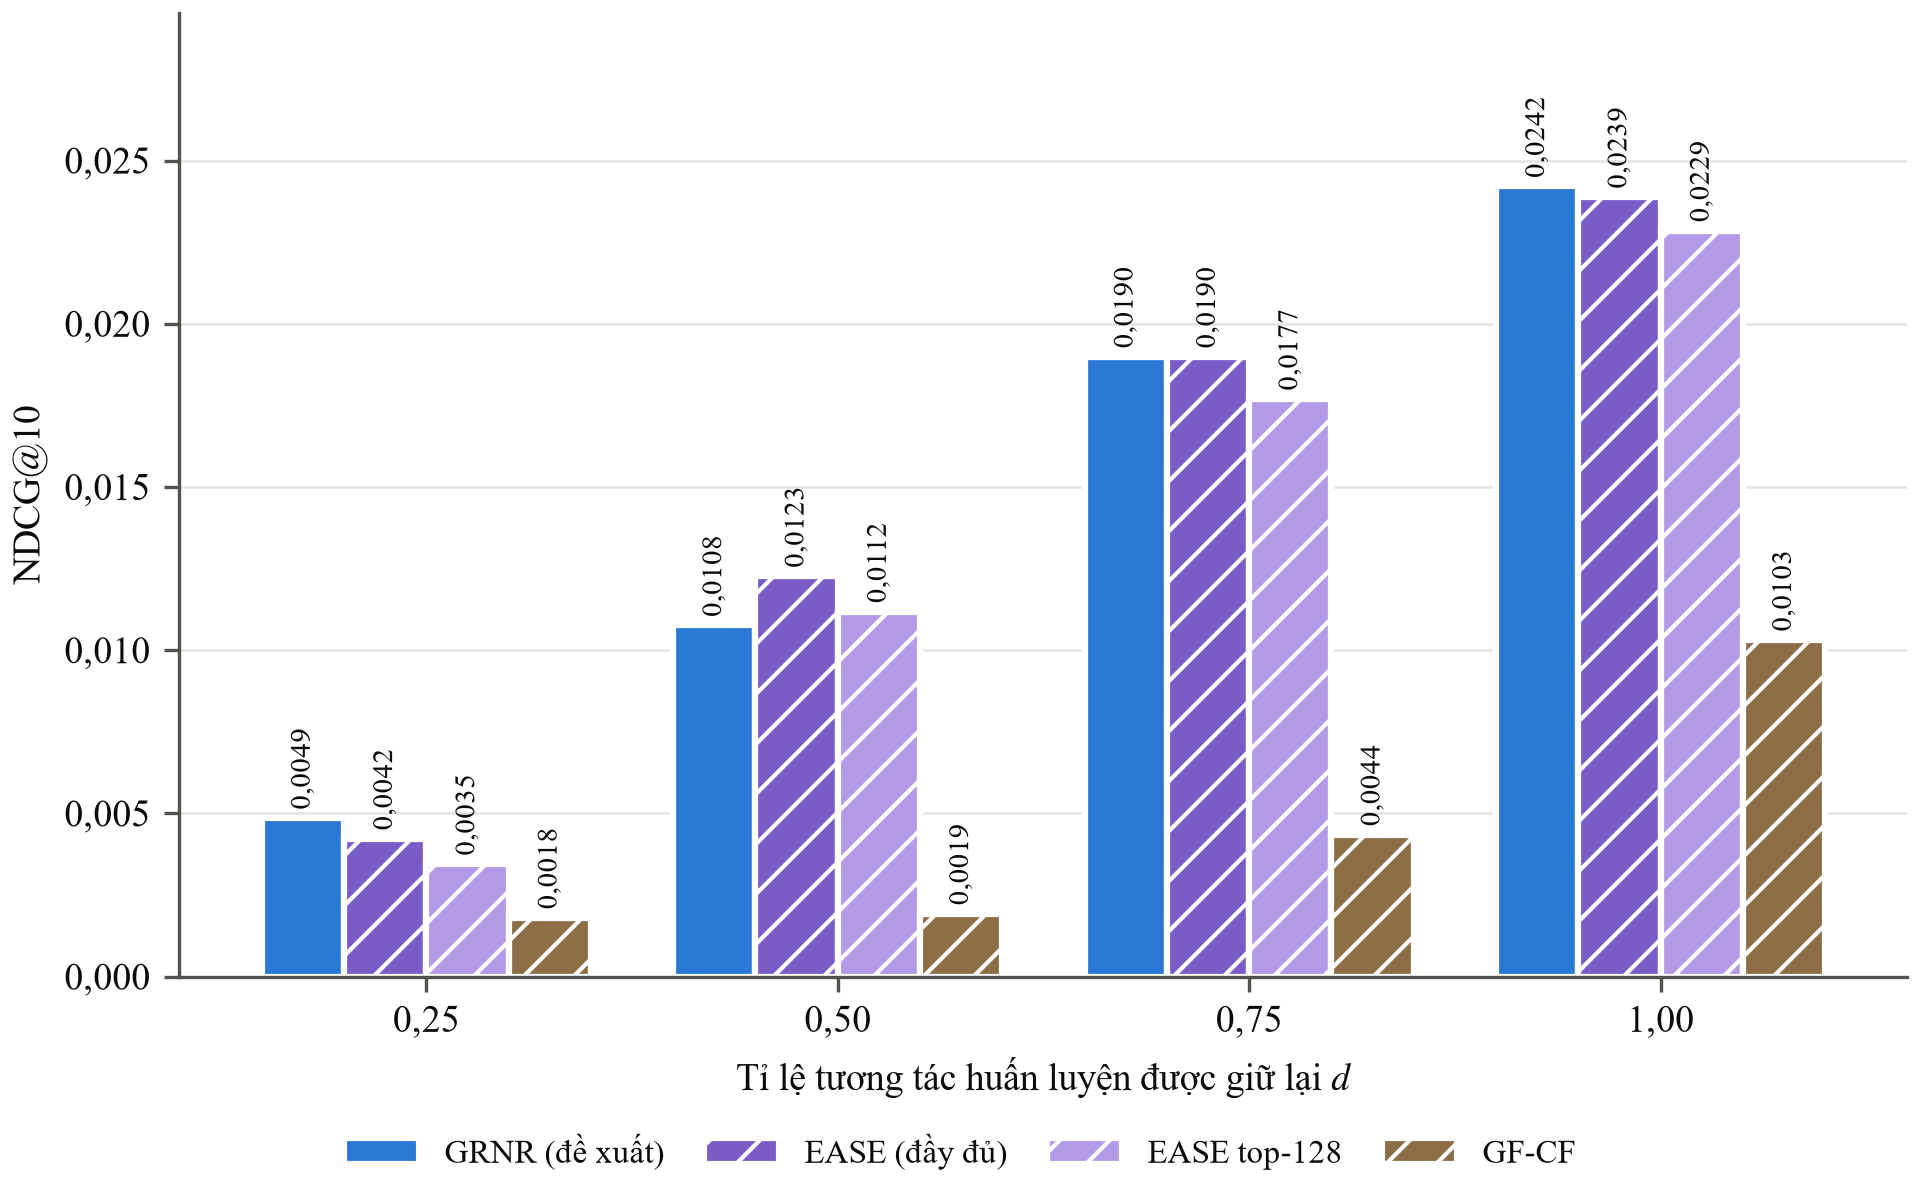
\includegraphics[width=0.75\linewidth]{H1_closed_form_density_ndcg10.png}
\caption{NDCG@10 theo mức $d$, nhóm giải trực tiếp}
\label{fig:closed-ndcg10}
\end{figure}

Mở rộng danh sách lên 20 vị trí như ở \figref{fig:closed-ndcg20} làm rõ thêm hai điều. Thứ nhất, ở $d=0{,}5$, GRNR vượt lại EASE top-128 nhưng vẫn kém EASE đầy đủ khoảng 0,0014, gần bằng mức kém ở NDCG@10. Thứ hai, ưu thế của GRNR ở mức thưa nhất tăng hơn gấp đôi, từ 0,00064 theo NDCG@10 lên 0,00146 theo NDCG@20. Vì hai thước đo chỉ khác nhau ở các vị trí từ 11 đến 20, phần lớn ưu thế này nằm ở nửa sau của danh sách chứ không ở mười gợi ý đầu. Riêng GF-CF còn tăng khi $d$ giảm từ 0,5 xuống 0,25, nhưng đó là vì mô hình đã chạm đáy từ trước, không phải dấu hiệu bền vững.

\begin{figure}[H]
\centering
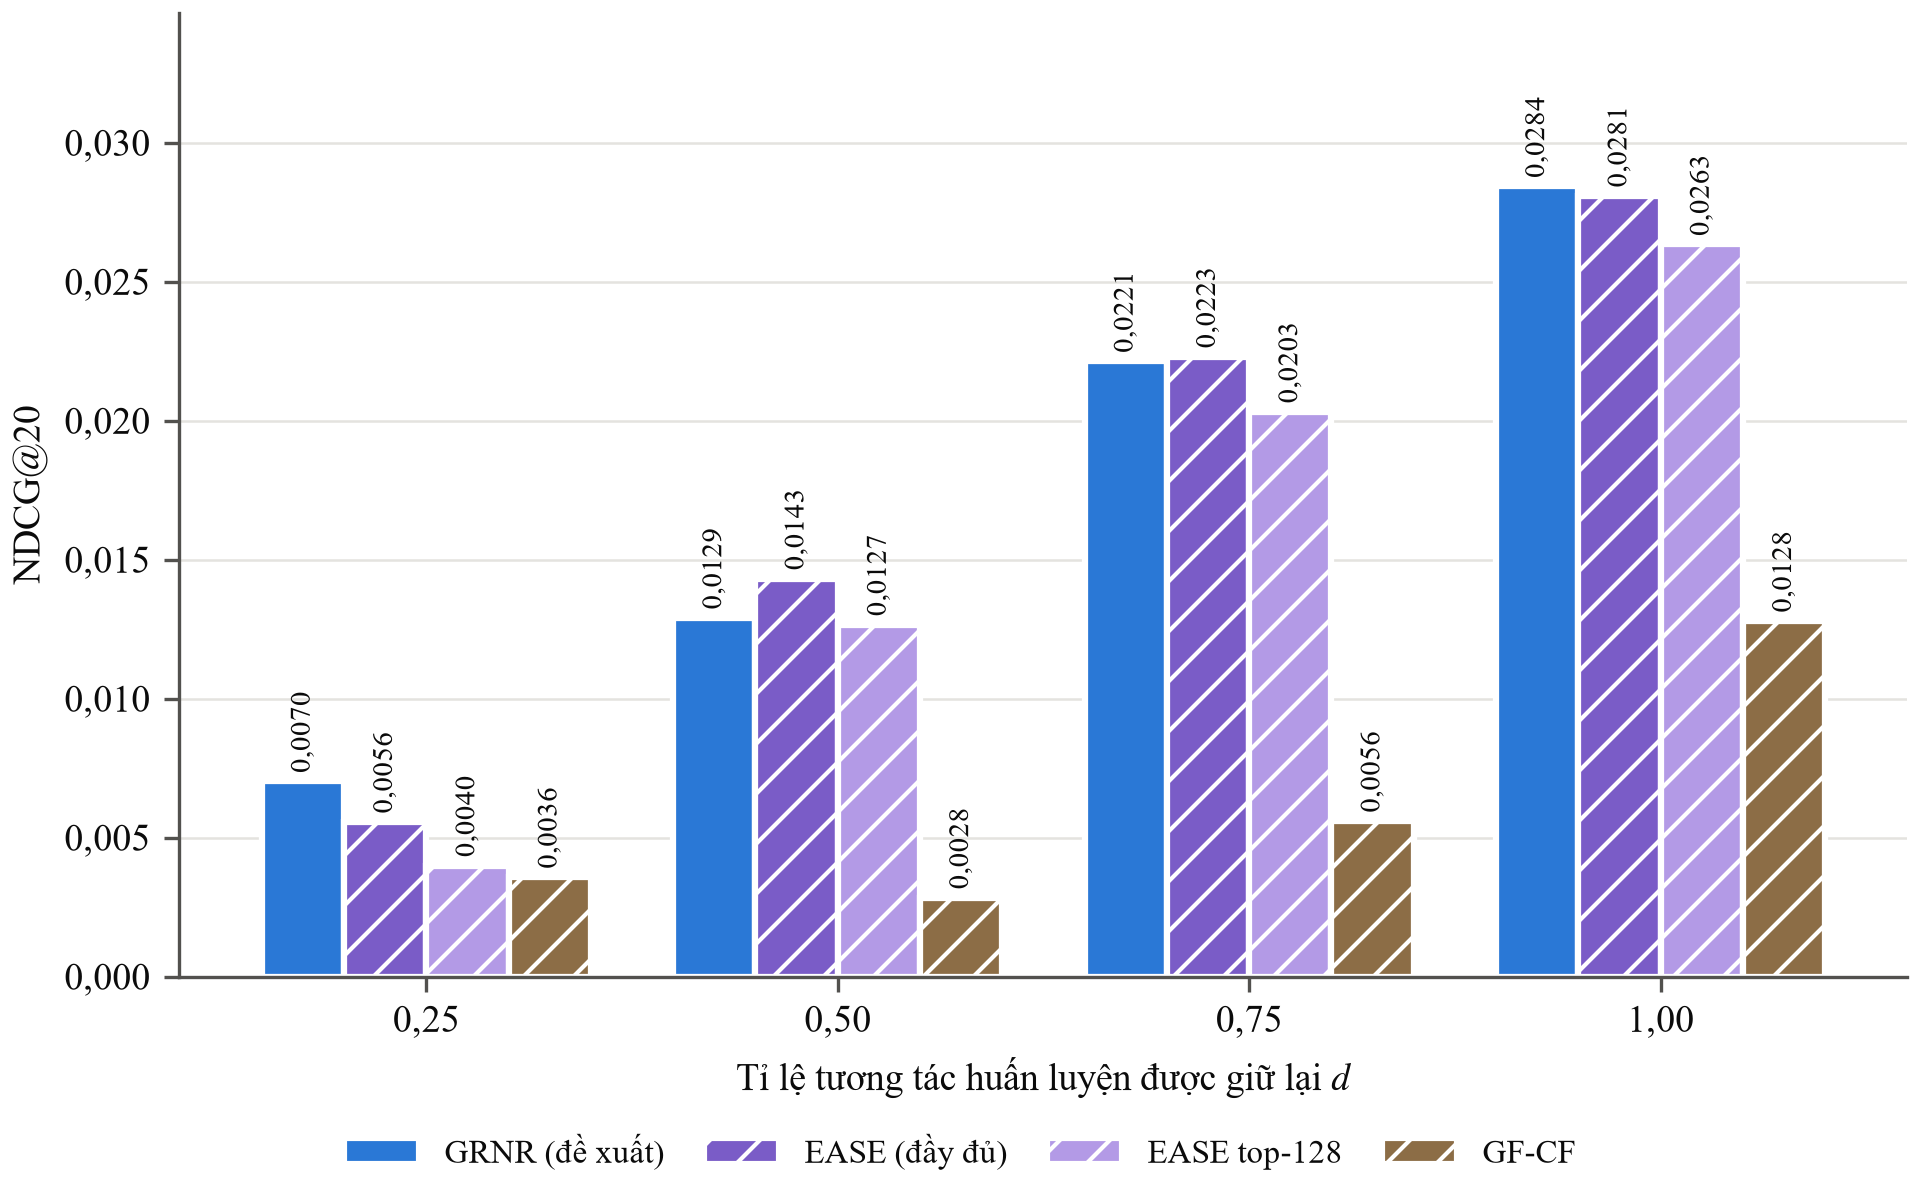
\includegraphics[width=0.75\linewidth]{H1_closed_form_density_ndcg20.png}
\caption{NDCG@20 theo mức $d$, nhóm giải trực tiếp}
\label{fig:closed-ndcg20}
\end{figure}

Recall bỏ qua vị trí và chỉ hỏi sản phẩm mục tiêu có lọt vào danh sách hay không, nhờ đó tách được câu hỏi ``có tìm thấy không'' khỏi câu hỏi ``có xếp đúng chỗ không''. \Figref{fig:closed-recall10} cho thấy hai thước đo không phải lúc nào cũng cùng chiều khi các mô hình đứng sát nhau: ở $d=0{,}75$, GRNR nhỉnh hơn EASE đầy đủ về Recall@10 dù kém một chút về NDCG@20. Ở $d=0{,}5$, GRNR vẫn xếp cuối trong ba mô hình hồi quy. Ở mức thưa nhất, GRNR hơn EASE đầy đủ 0,00229, gấp khoảng ba lần mức chênh theo NDCG@10.

\begin{figure}[H]
\centering
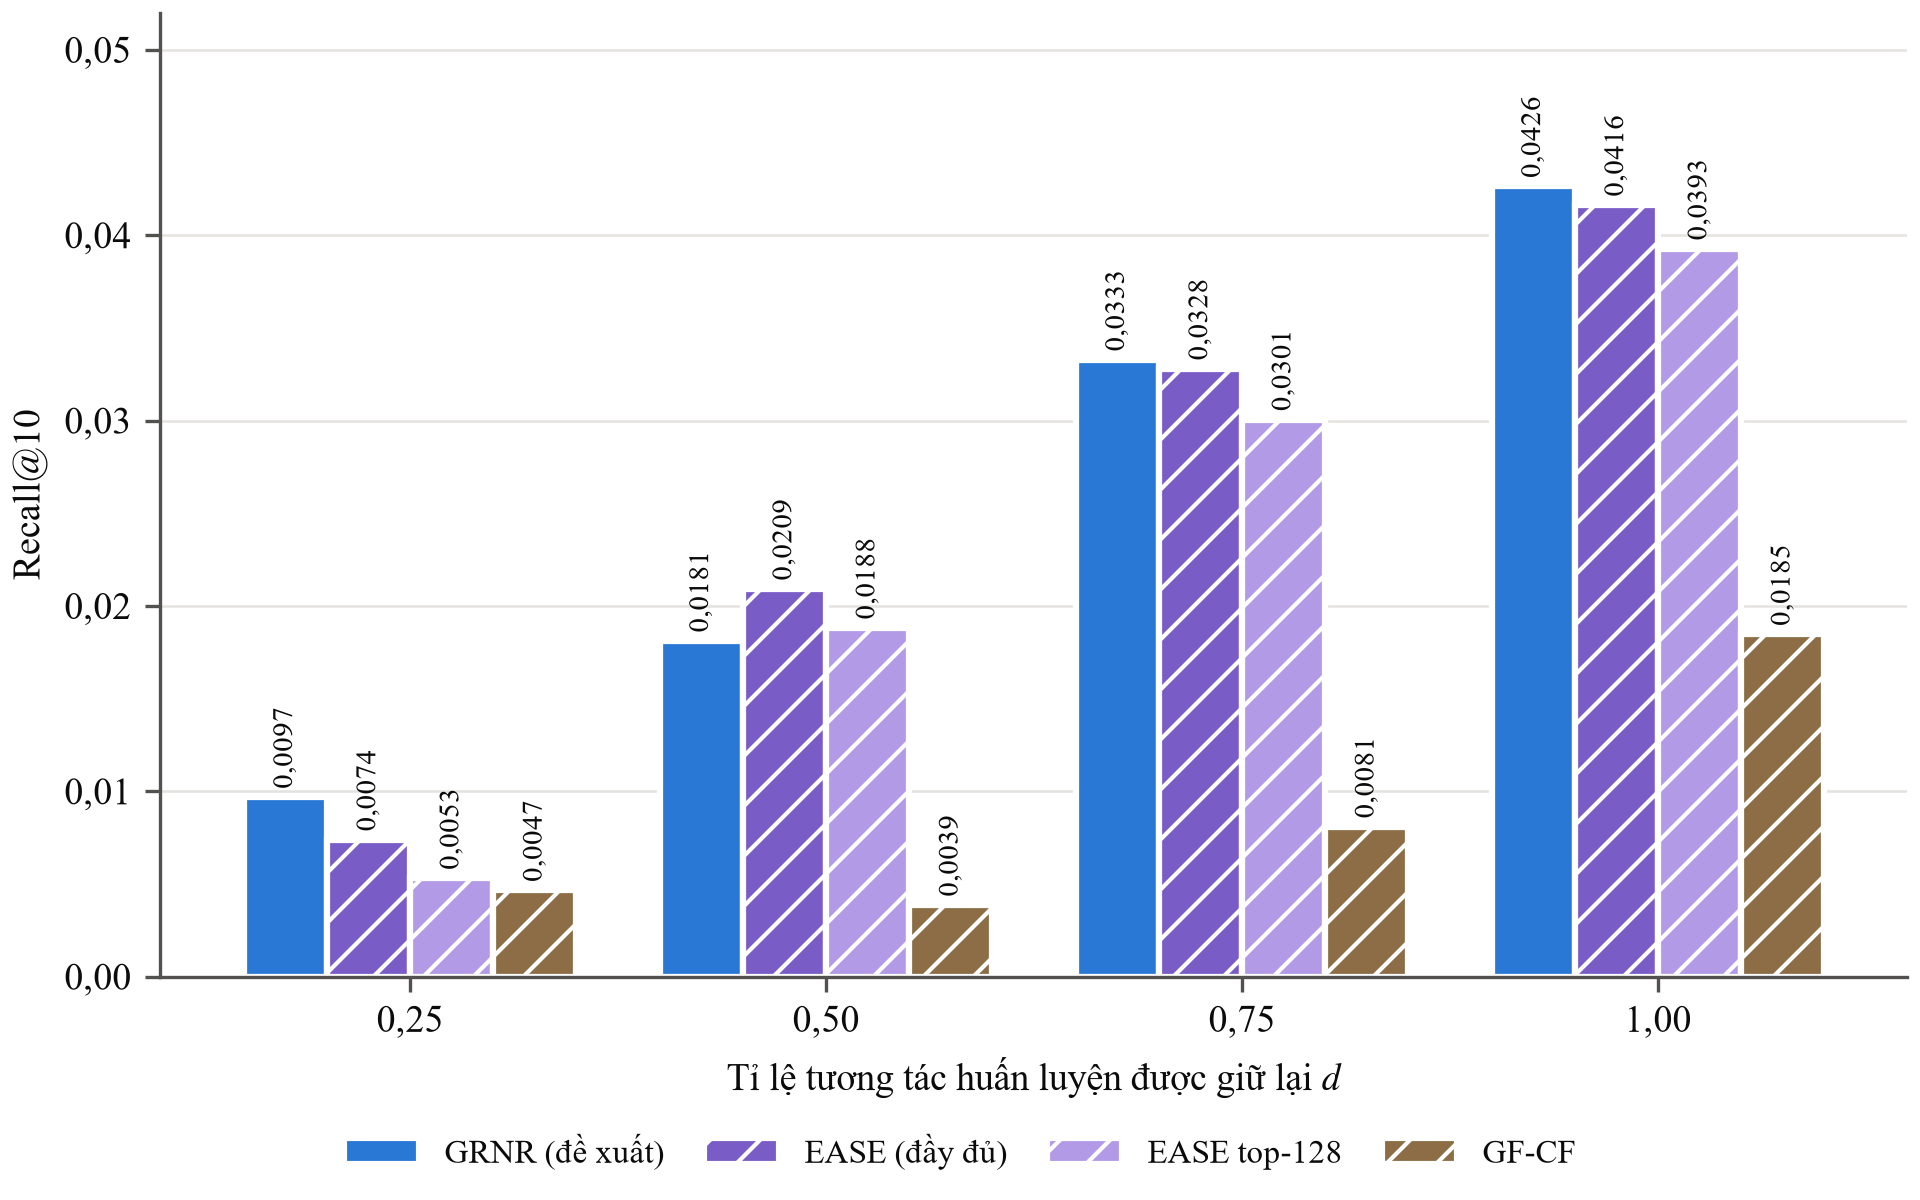
\includegraphics[width=0.75\linewidth]{H1_closed_form_density_recall10.png}
\caption{Recall@10 theo mức $d$, nhóm giải trực tiếp}
\label{fig:closed-recall10}
\end{figure}

Recall@20 ở \figref{fig:closed-recall20} khuếch đại cùng xu hướng. Ở mức thưa nhất, GRNR đạt 0,01834, hơn EASE đầy đủ 0,0056; ở $d=0{,}5$, GRNR lại vượt EASE top-128 như ở NDCG@20. Các quan sát này chỉ về cùng một hướng: danh sách càng dài, GRNR càng tìm thêm được mục tiêu ở các hạng sau, nhưng điều đó chưa có nghĩa là mô hình đưa mục tiêu lên đầu danh sách tốt hơn. GF-CF một lần nữa hành xử bất thường: Recall@20 của nó tăng khi bớt dữ liệu và ở mức thưa nhất còn vượt EASE top-128, thêm một dấu hiệu cho thấy baseline này cần được kiểm tra lại.

\begin{figure}[H]
\centering
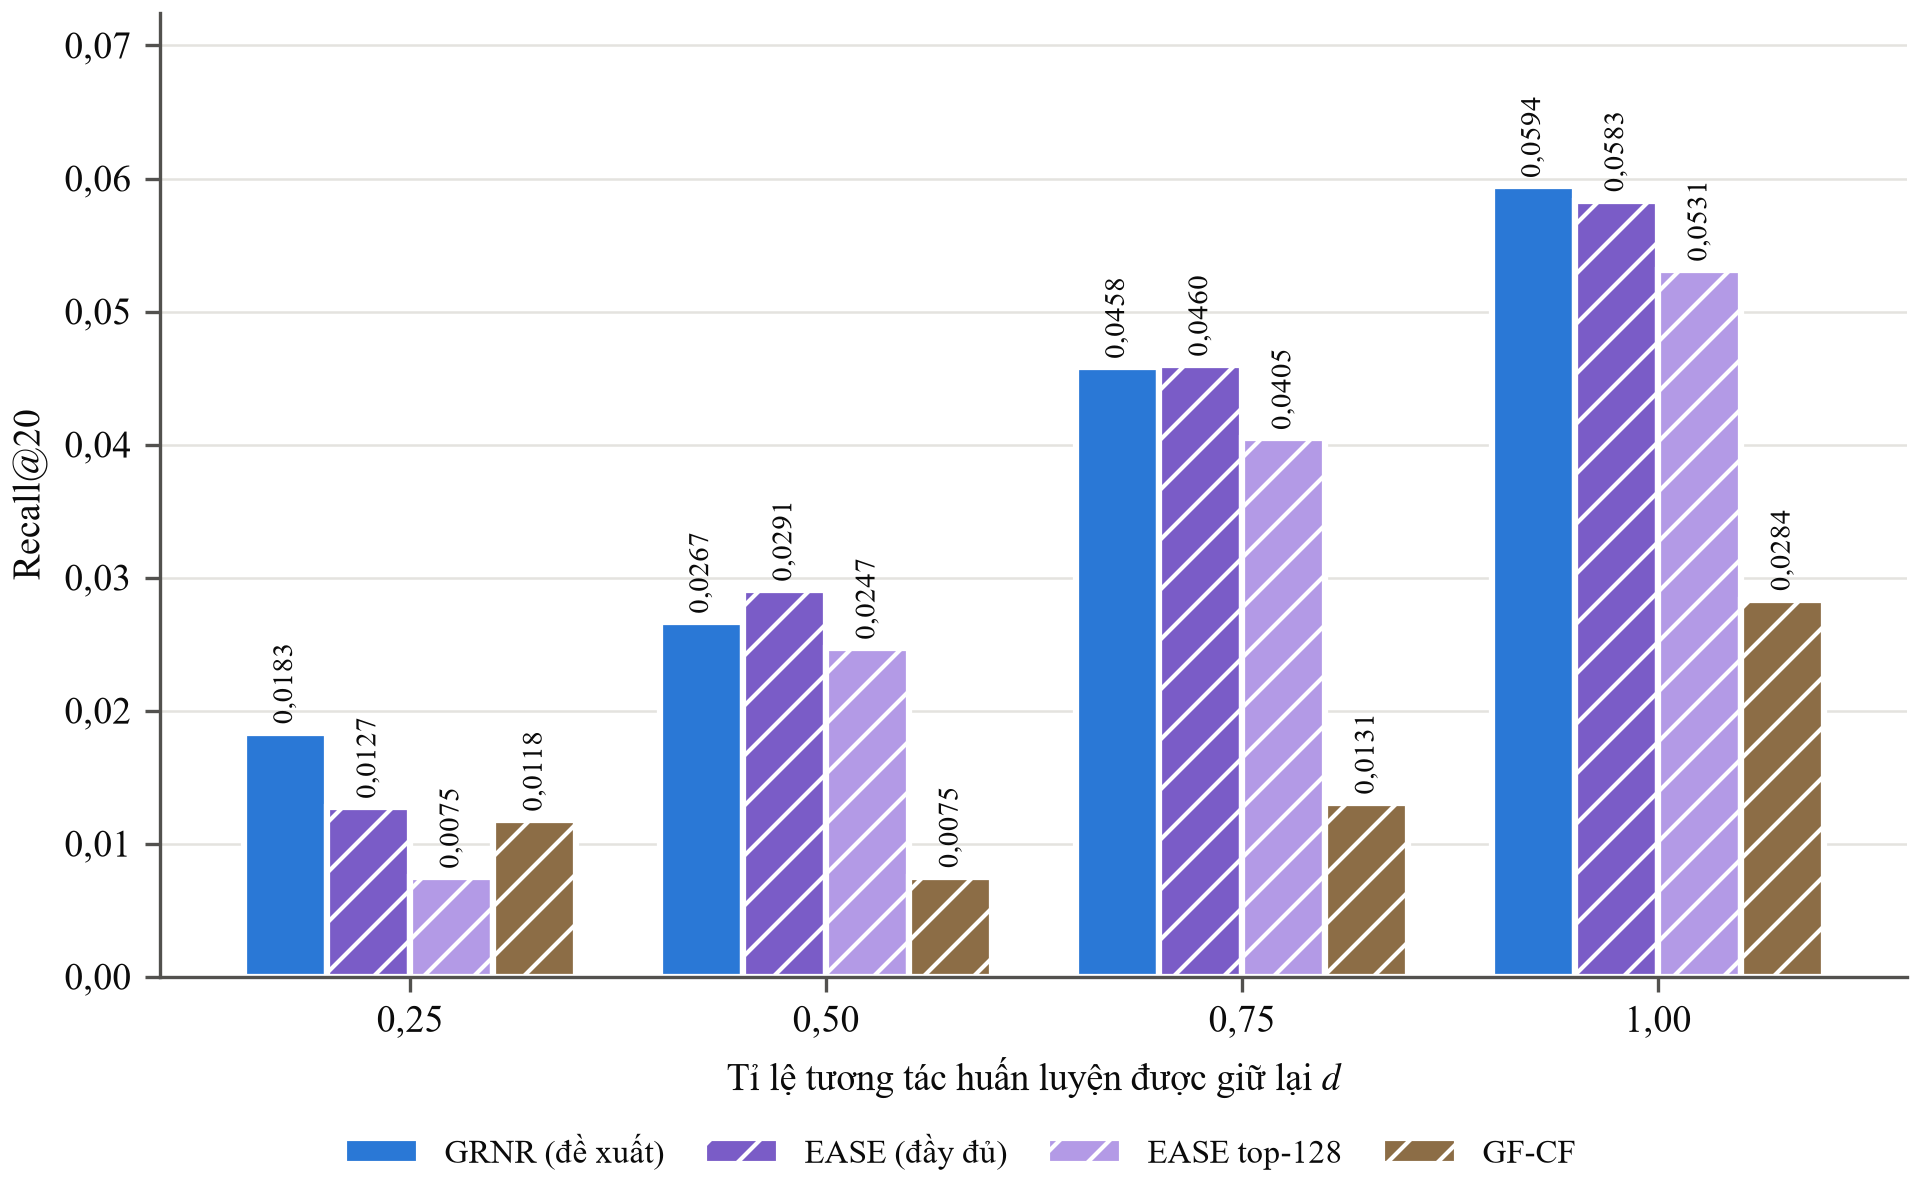
\includegraphics[width=0.75\linewidth]{H1_closed_form_density_recall20.png}
\caption{Recall@20 theo mức $d$, nhóm giải trực tiếp}
\label{fig:closed-recall20}
\end{figure}

Đường NDCG@K ở \figref{fig:closed-at-k} cho biết khoảng cách giữa các mô hình nằm ở đầu hay cuối danh sách. Khi $d\ge0{,}75$, đường của GRNR và EASE đầy đủ chồng lên nhau ngay từ gợi ý đầu tiên, còn EASE top-128 chỉ tách xuống ở các vị trí sau. Ở $d=0{,}5$, EASE đầy đủ dẫn từ đầu đến cuối danh sách. Ở mức thưa nhất, GRNR thậm chí kém EASE đầy đủ ở các vị trí đầu, với NDCG@1 bằng 0,00167 so với 0,00194, rồi bắt kịp quanh vị trí thứ năm và vượt lên sau đó, đúng như khác biệt giữa NDCG@10 và NDCG@20 đã gợi ý. Các đường được tính từ cùng danh sách dự đoán nên chỉ mang tính mô tả; kiểm định chính vẫn dành cho NDCG@20.

\begin{figure}[H]
\centering
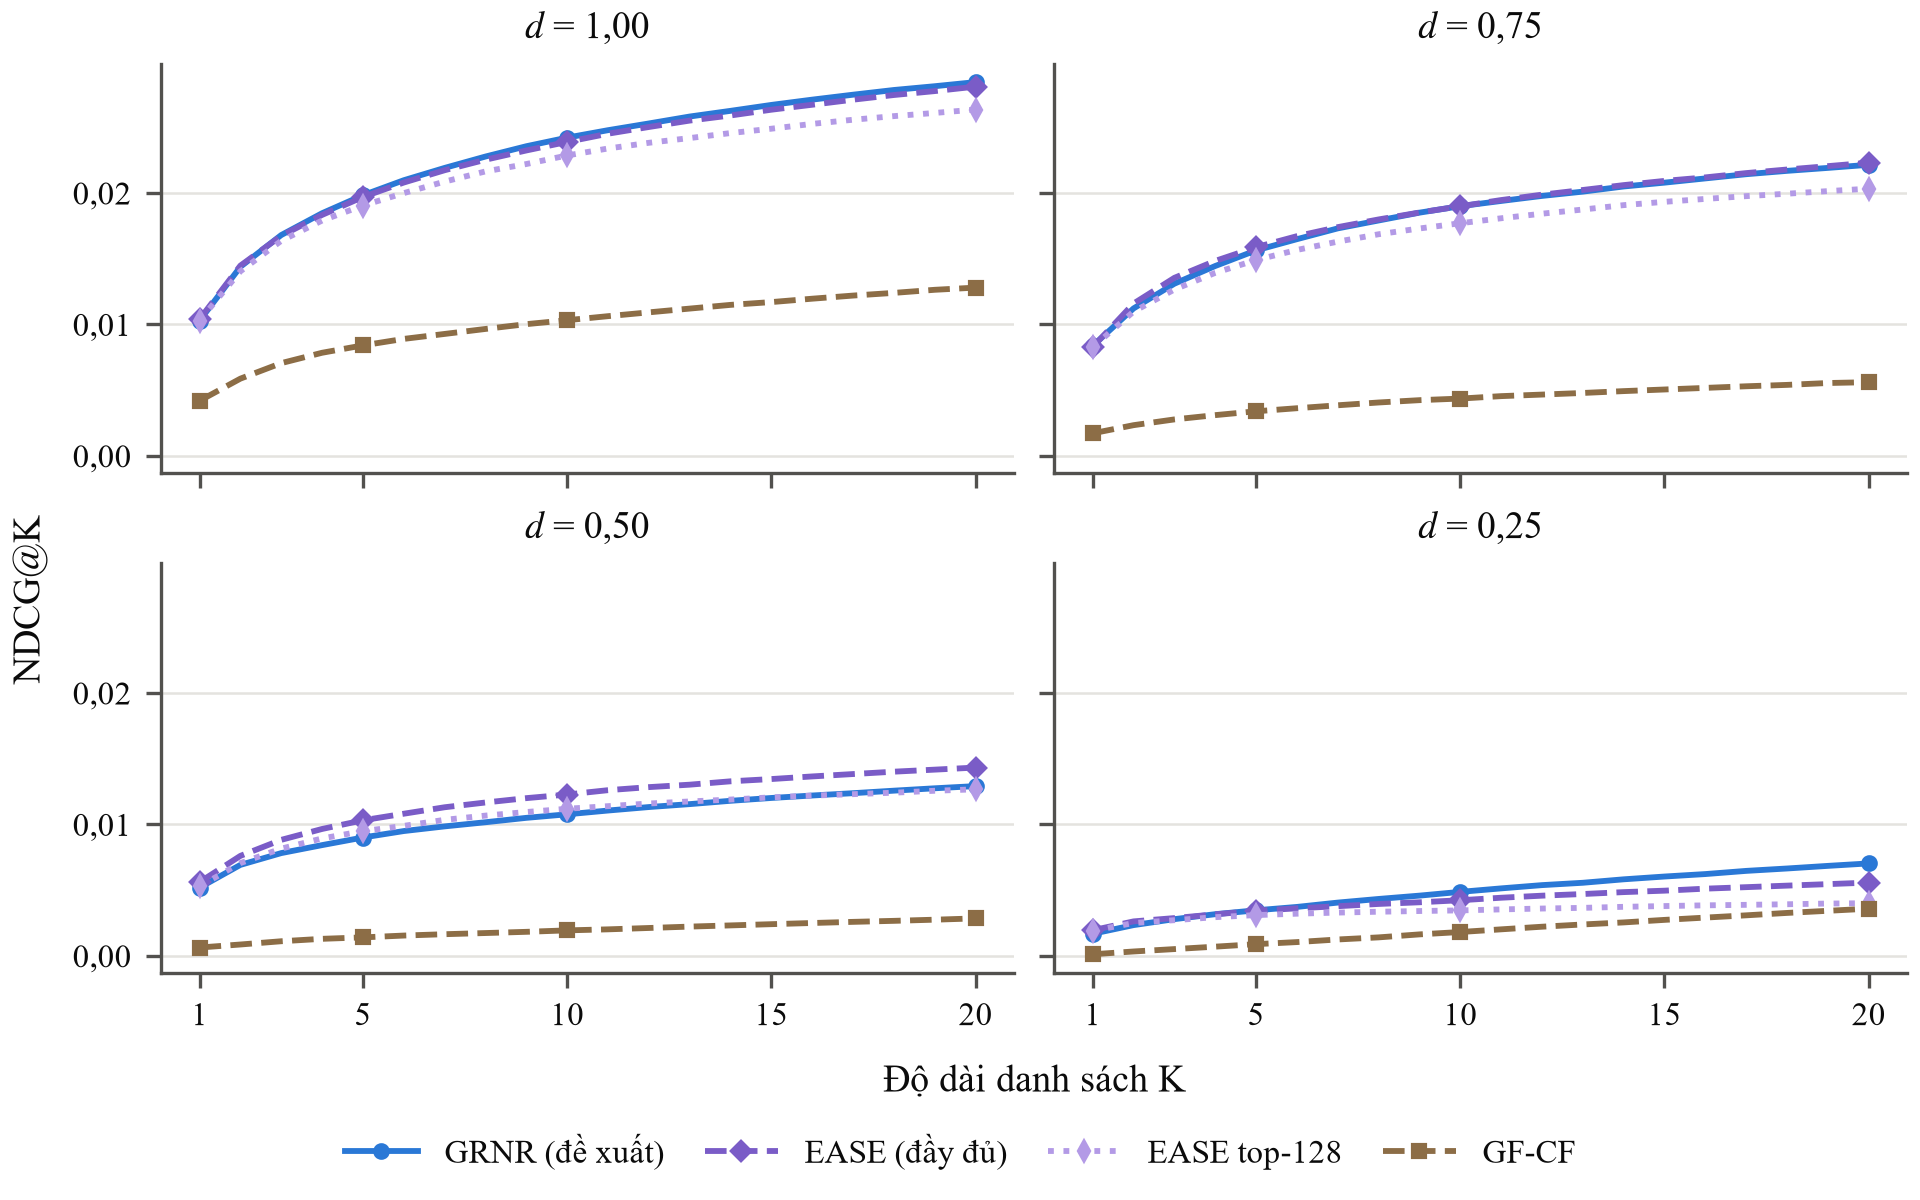
\includegraphics[width=0.75\linewidth]{H8_closed_form_ndcg_at_k.png}
\caption{NDCG@K, nhóm giải trực tiếp}
\label{fig:closed-at-k}
\end{figure}

\FloatBarrier
\subsubsection{Chất lượng khi dữ liệu thưa dần}

Nếu chỉ so các mô hình với nhau, diễn biến theo mức thưa khá rối. Theo \tabref{tab:closed-form-sig}, GRNR chưa phân định được với EASE đầy đủ ở $d=1$ và $d=0{,}75$, thua rõ ở $d=0{,}5$ với khoảng tin cậy nằm hẳn dưới 0, rồi thắng ở mức thưa nhất. Ở $d=0{,}5$, GRNR cũng không hơn được EASE top-128. Đây là kết quả bất lợi cho GRNR, và kiểm định một phía không phát hiện được nó vì chỉ được thiết kế để tìm chiều GRNR tốt hơn; phải đọc khoảng tin cậy mới thấy.

Khi đặt thêm mốc MostPop vào như ở \figref{fig:closed-density} thì một xu hướng lớn hơn nhiều hiện ra: cả nhóm cùng rơi xuống dưới mức xếp hạng theo độ phổ biến.

\begin{figure}[H]
\centering
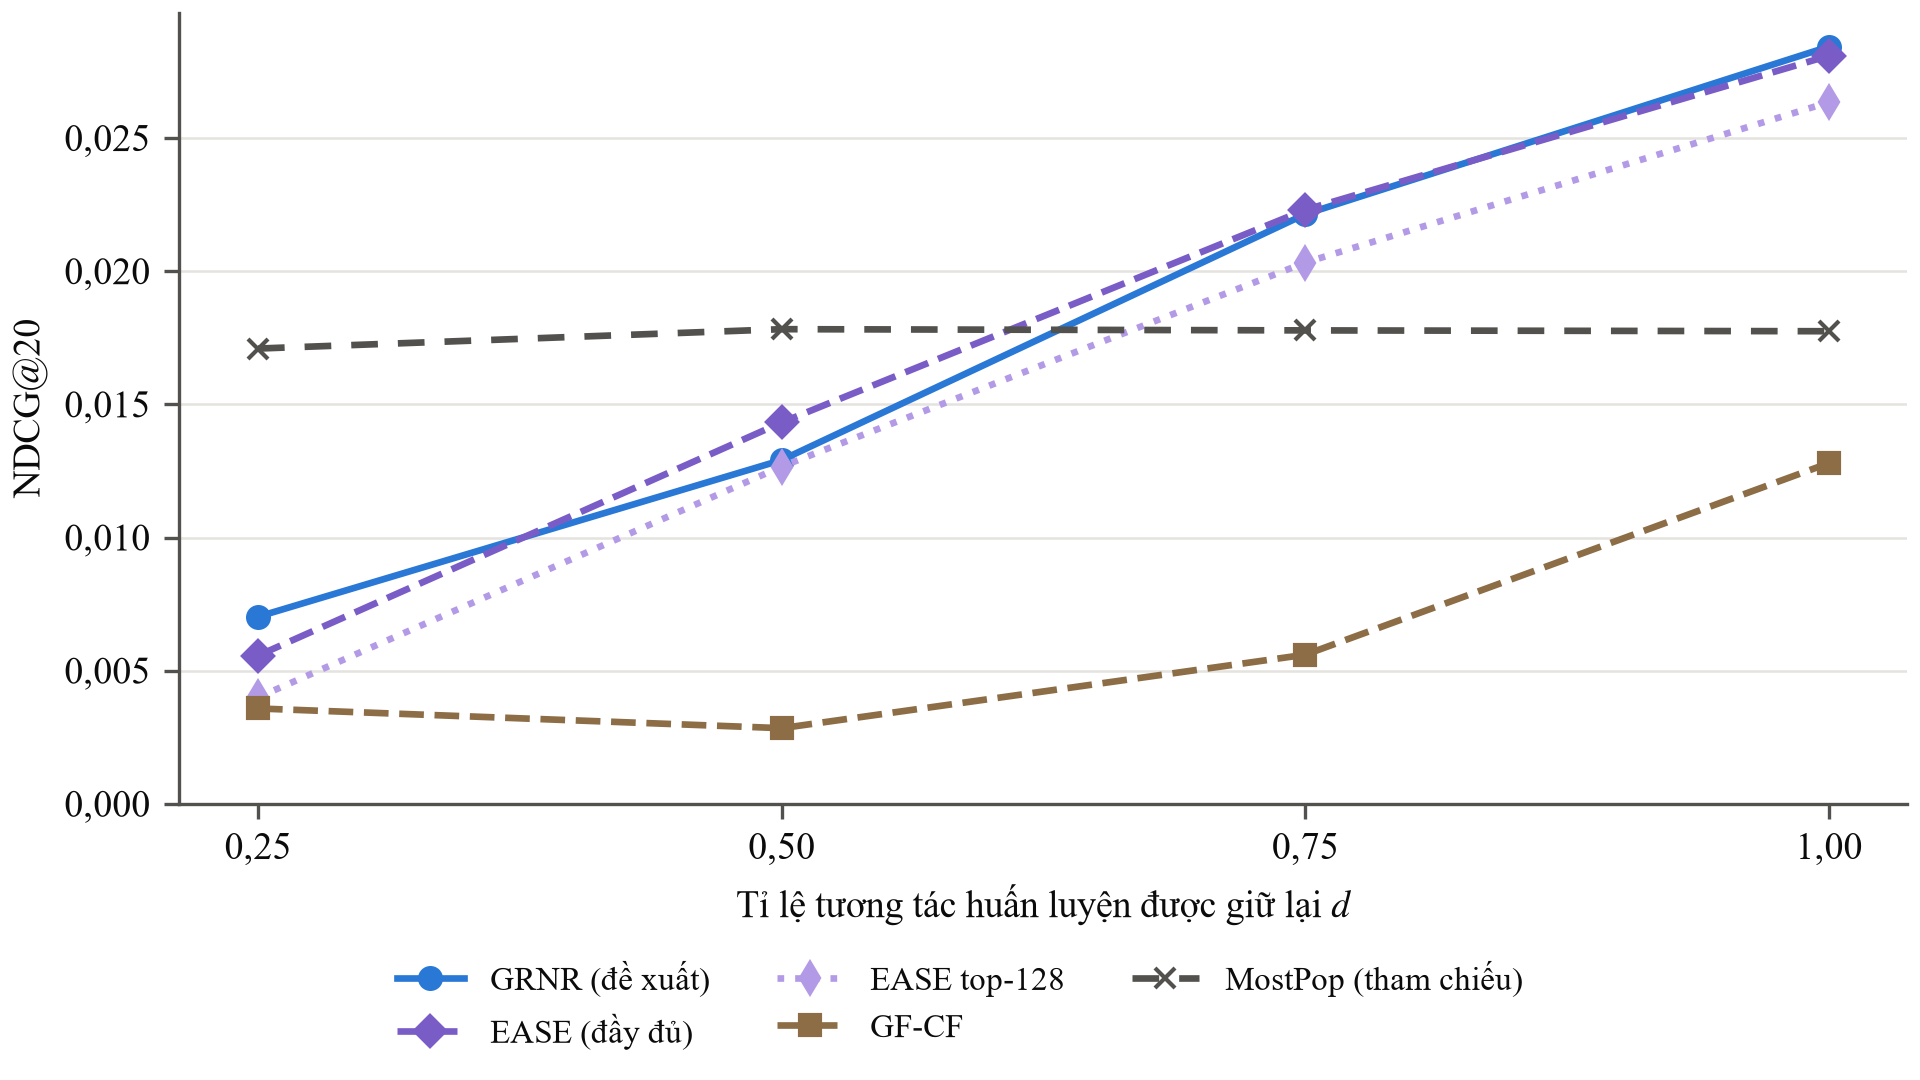
\includegraphics[width=0.75\linewidth]{H9_mostpop_closed_ndcg20.png}
\caption{NDCG@20 so với MostPop, nhóm giải trực tiếp}
\label{fig:closed-density}
\end{figure}

\Tabref{tab:closed-gain} lượng hóa xu hướng này bằng mức vượt MostPop, tức chênh lệch tương đối so với cách xếp hạng không cá nhân hóa. Khi có đủ dữ liệu, ba mô hình hồi quy vượt MostPop từ 49\% đến 60\%. Mức vượt giảm còn 14--26\% ở $d=0{,}75$ rồi đổi dấu: ở $d=0{,}5$, cả ba đã thấp hơn MostPop 20--29\%, và ở mức thưa nhất thấp hơn 59--77\%. GF-CF thấp hơn MostPop ở cả bốn mức. Mức sụt này lớn hơn cả một bậc so với khoảng cách vài phần trăm giữa các mô hình trong nhóm.

\begin{table}[H]
\centering
\small
\begin{tabular}{@{}lrrrr@{}}
\toprule
& $d=1$ & $d=0{,}75$ & $d=0{,}5$ & $d=0{,}25$ \\
\midrule
MostPop (NDCG@20) & 0{,}01775 & 0{,}01778 & 0{,}01782 & 0{,}01710 \\
\midrule
GRNR & $+60{,}2\%$ & $+24{,}5\%$ & $-27{,}6\%$ & $-58{,}9\%$ \\
EASE đầy đủ & $+58{,}3\%$ & $+25{,}5\%$ & $-19{,}7\%$ & $-67{,}4\%$ \\
EASE top-128 & $+48{,}5\%$ & $+14{,}3\%$ & $-28{,}9\%$ & $-76{,}6\%$ \\
GF-CF & $-27{,}9\%$ & $-68{,}5\%$ & $-84{,}1\%$ & $-79{,}1\%$ \\
\bottomrule
\end{tabular}
\caption{Mức vượt MostPop, nhóm giải trực tiếp}
\label{tab:closed-gain}
\end{table}

Tỉ lệ duy trì nhìn cùng dữ liệu từ một góc khác: chất lượng ở mỗi mức được tính thành phần trăm của chính mô hình đó ở $d=1$, nên cho biết mô hình suy giảm nhanh hay chậm, bất kể xuất phát cao hay thấp. Theo NDCG@10 ở \figref{fig:closed-retention-ndcg10}, ba mô hình hồi quy suy giảm gần như đều nhau ở $d=0{,}75$, cùng giữ 77--80\%. Ở $d=0{,}5$, GRNR giảm nhanh hơn, chỉ còn 44,5\% so với 49--51\% của hai biến thể EASE; nhưng ở mức thưa nhất, thứ tự đảo lại và GRNR giữ nhiều nhất, 20,1\%. GF-CF mất hơn một nửa chất lượng ngay ở bước giảm đầu tiên.

\begin{figure}[H]
\centering
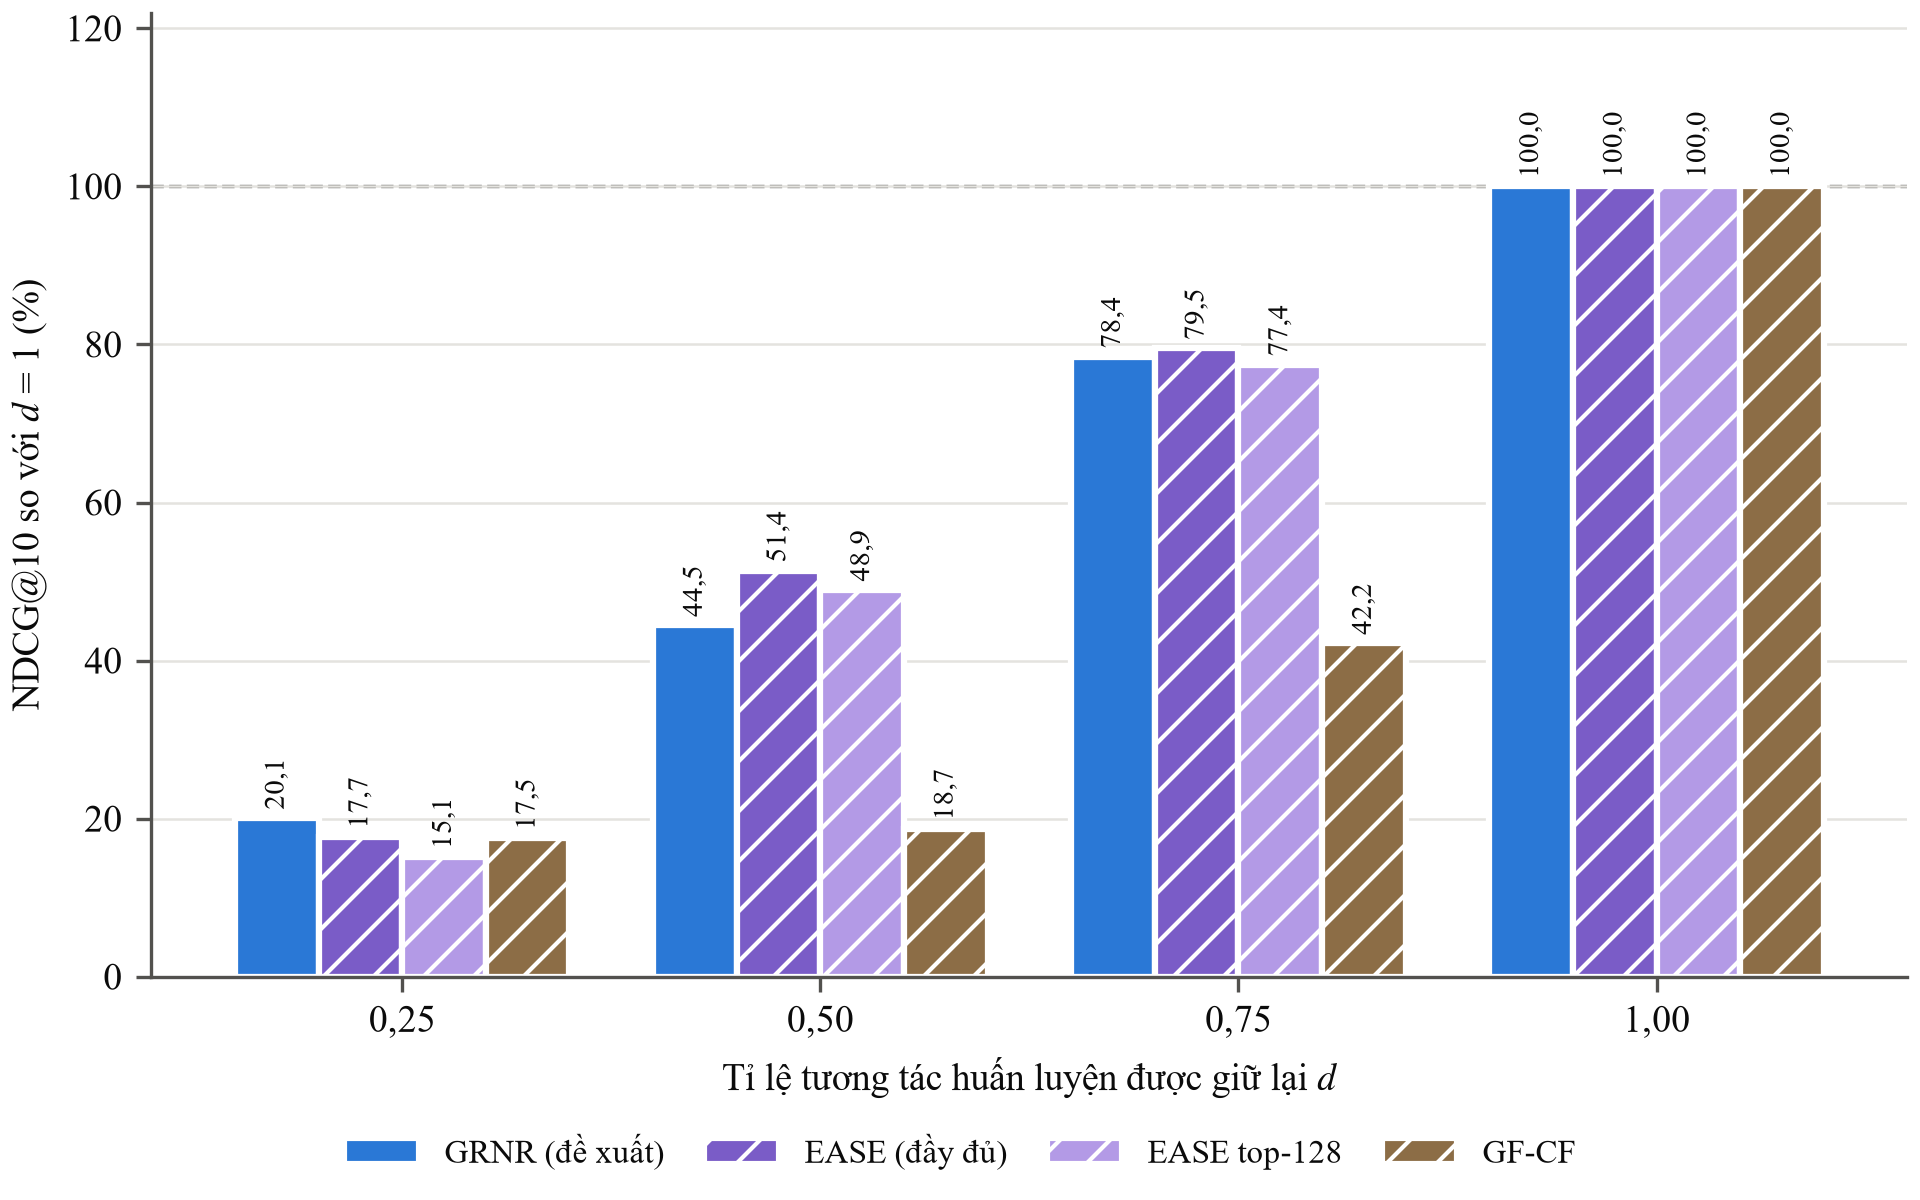
\includegraphics[width=0.75\linewidth]{H4_closed_form_retention_ndcg10.png}
\caption{Tỉ lệ duy trì NDCG@10, nhóm giải trực tiếp}
\label{fig:closed-retention-ndcg10}
\end{figure}

NDCG@20 ở \figref{fig:closed-retention-ndcg20} cho cùng diễn biến, với GRNR giữ 24,7\% ở mức thưa nhất, nhiều nhất trong ba mô hình hồi quy. Tỉ lệ 28,0\% của GF-CF còn cao hơn, nhưng con số này dễ gây hiểu lầm: nó đến từ việc mô hình đã chạm đáy ở $d=0{,}5$ rồi nhích lên, chứ không phải từ sức bền. Hiện tượng này, cùng việc thời gian chạy của GF-CF không tăng đều theo lượng dữ liệu, chưa được giải thích.

\begin{figure}[H]
\centering
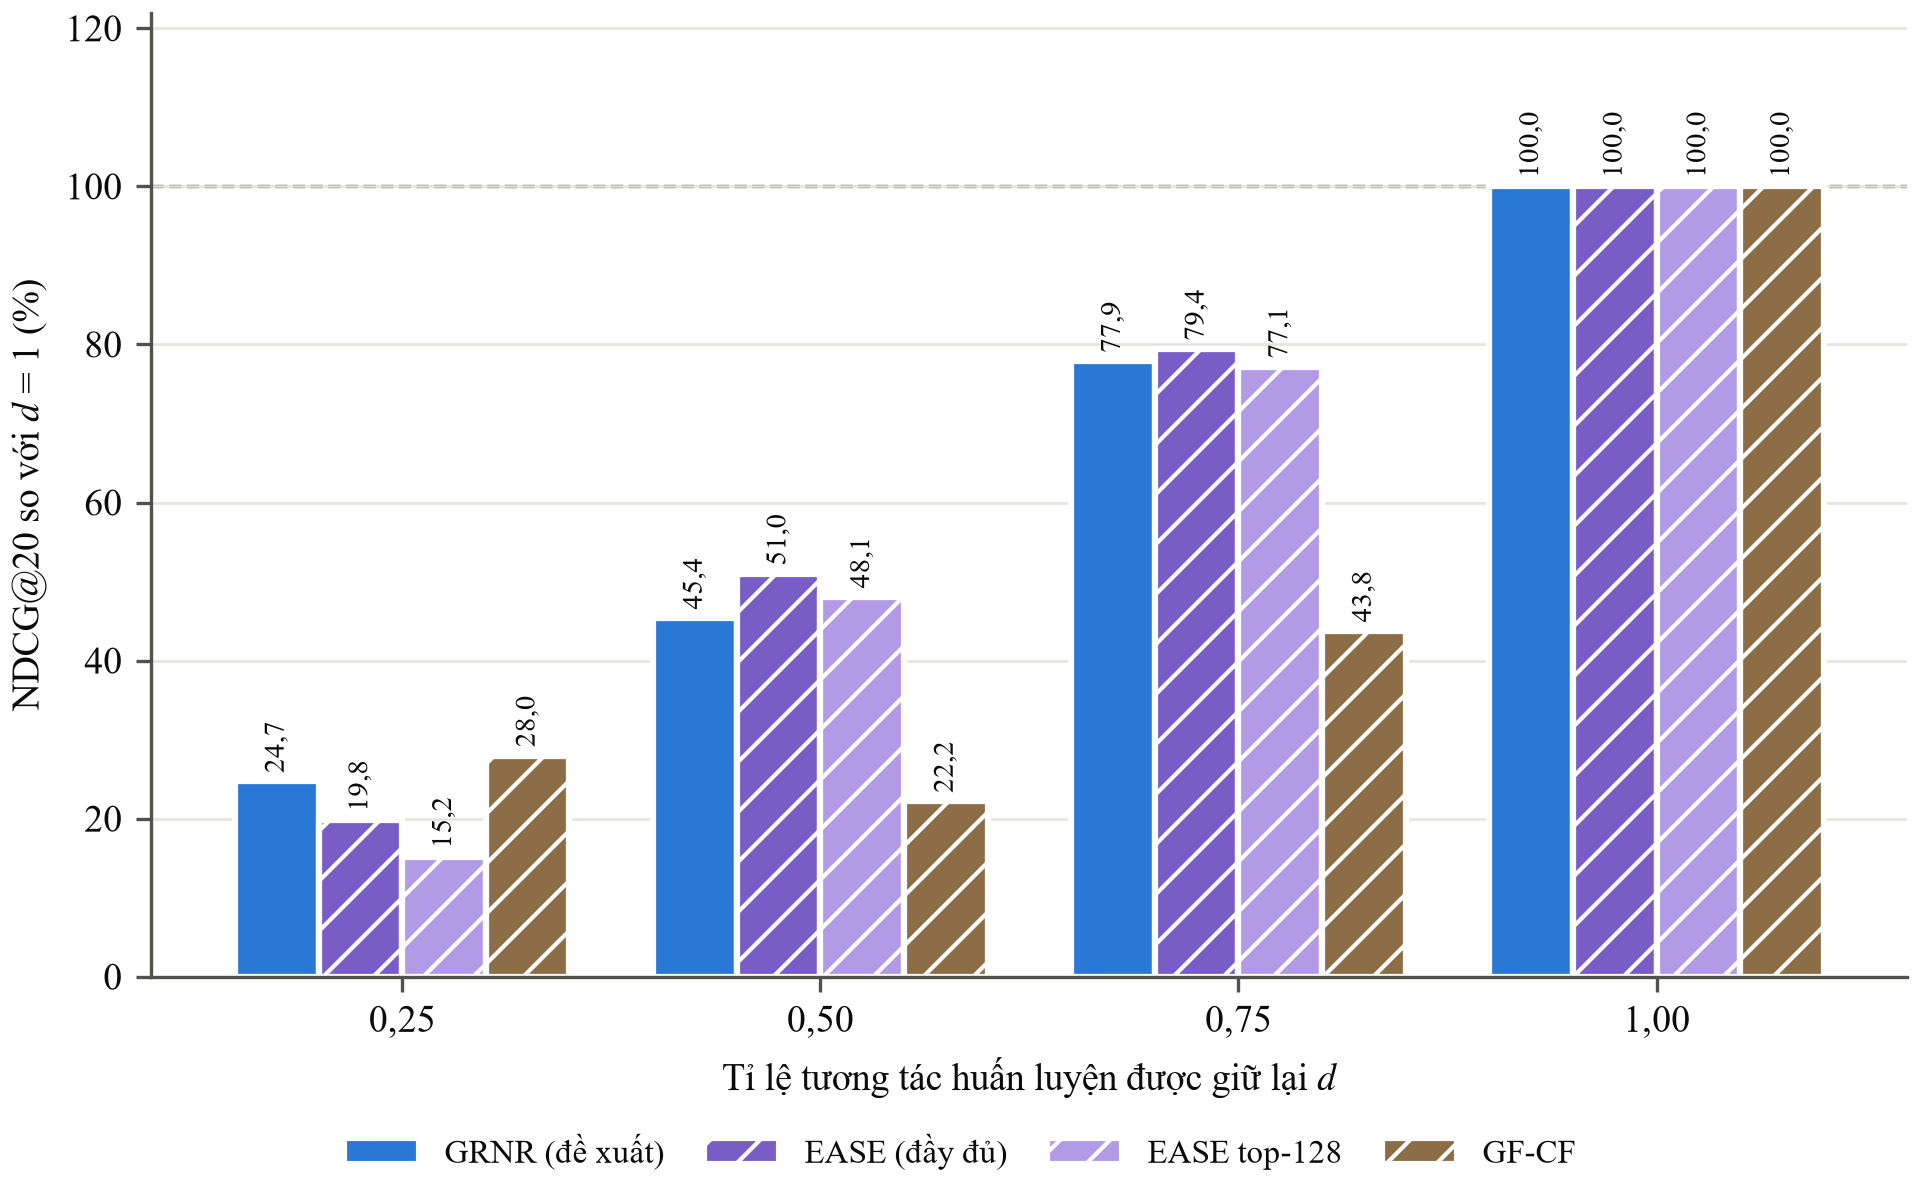
\includegraphics[width=0.75\linewidth]{H4_closed_form_retention_ndcg20.png}
\caption{Tỉ lệ duy trì NDCG@20, nhóm giải trực tiếp}
\label{fig:closed-retention-ndcg20}
\end{figure}

Recall@10 ở \figref{fig:closed-retention-recall10} lặp lại mẫu hình đó: GRNR giảm nhanh hơn hai biến thể EASE ở $d=0{,}5$ nhưng giữ nhiều nhất trong ba mô hình hồi quy ở mức thưa nhất. Khoảng cách đáng chú ý nhất lúc này là giữa GRNR và EASE top-128, gần 9 điểm phần trăm, nên bản EASE bị cắt là mô hình chịu thiệt nhiều nhất khi dữ liệu cạn.

\begin{figure}[H]
\centering
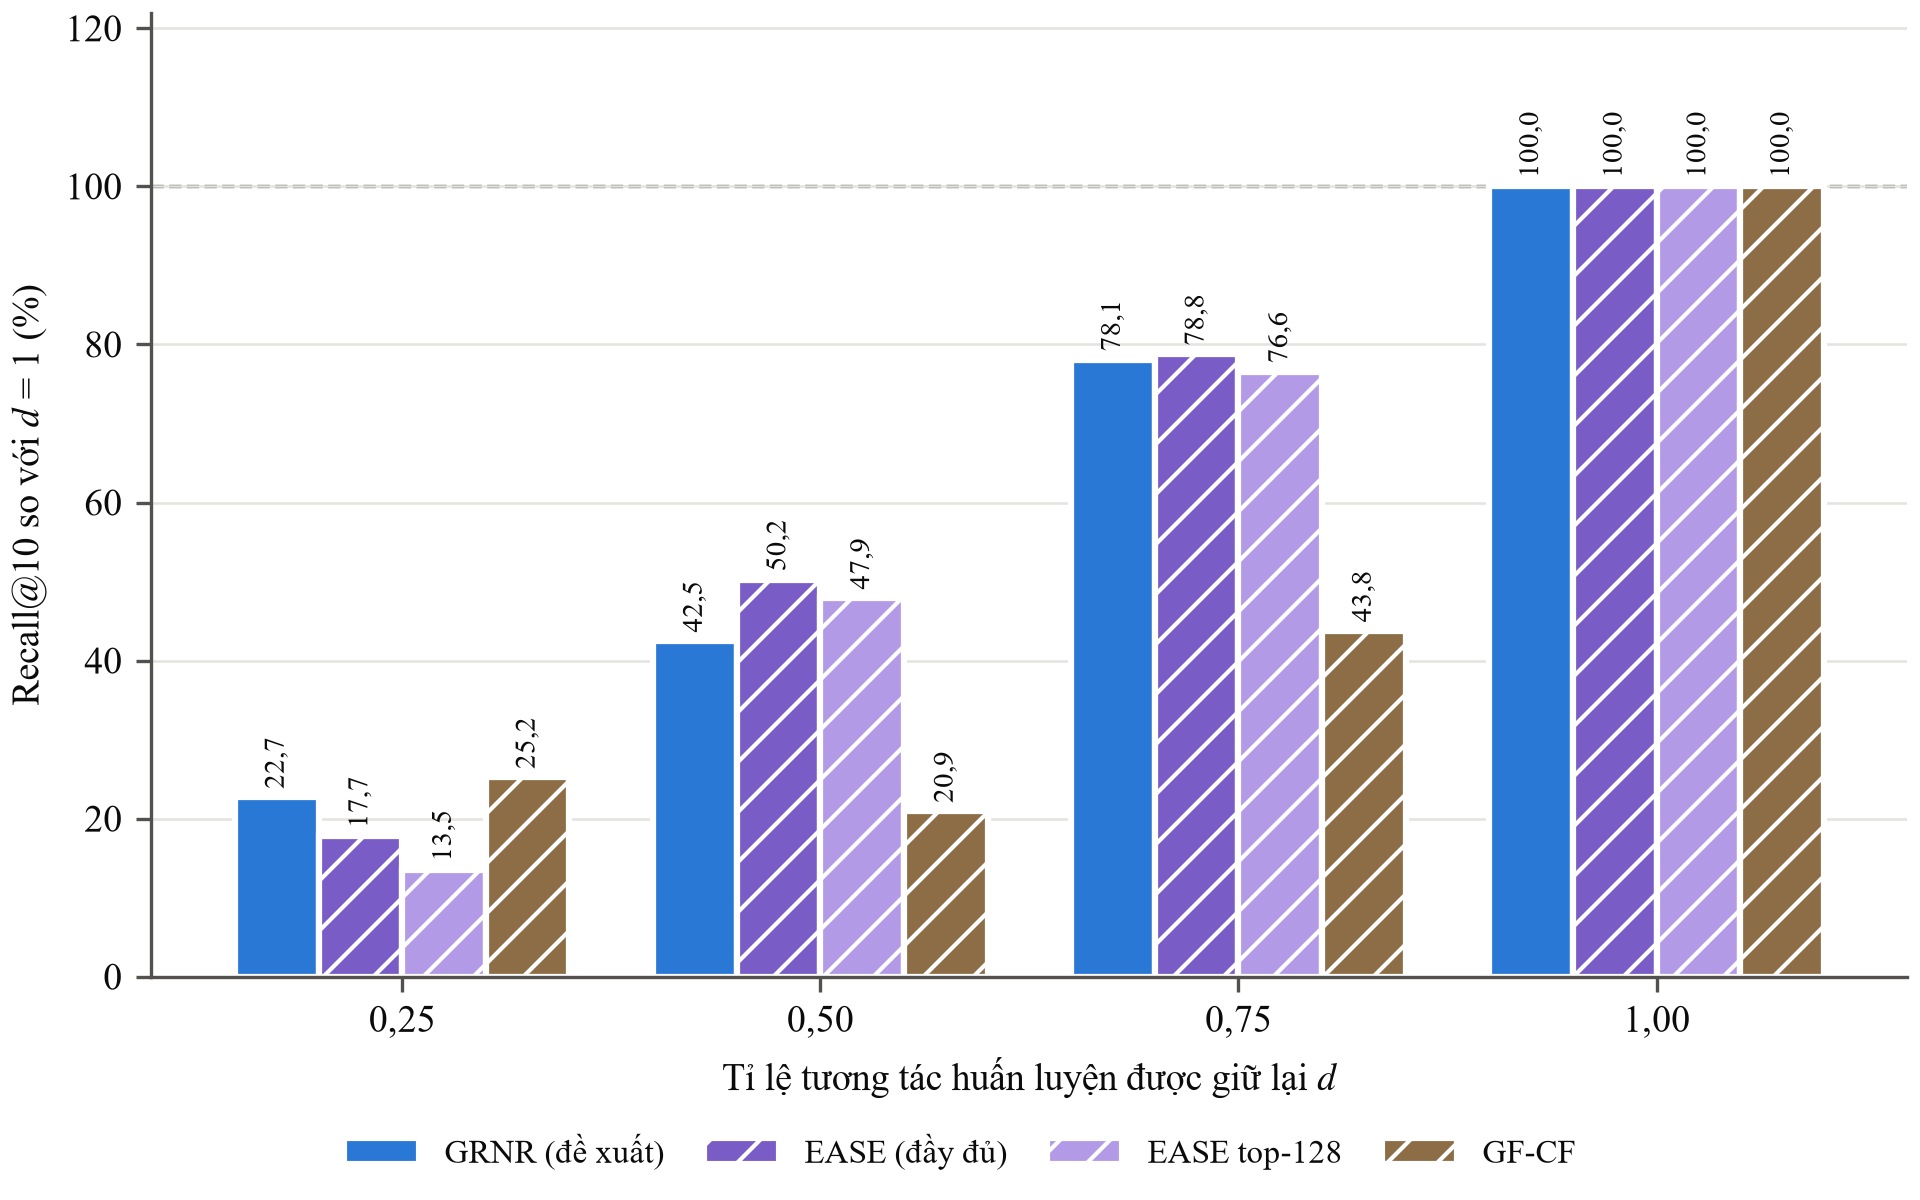
\includegraphics[width=0.75\linewidth]{H4_closed_form_retention_recall10.png}
\caption{Tỉ lệ duy trì Recall@10, nhóm giải trực tiếp}
\label{fig:closed-retention-recall10}
\end{figure}

Recall@20 ở \figref{fig:closed-retention-recall20} là thước đo duy nhất mà GRNR còn giữ được gần một phần ba giá trị ban đầu ở mức thưa nhất, 30,9\% so với 24,7\% theo NDCG@20. Mô hình vẫn đưa được một phần mục tiêu vào 20 vị trí đầu, nhưng phần chất lượng phụ thuộc vào vị trí suy giảm mạnh hơn. GF-CF có tỉ lệ cao nhất, 41,5\%, cũng chỉ vì Recall@20 của nó tăng lên khi bớt dữ liệu. Vì mỗi mô hình có một mẫu số riêng, các tỉ lệ duy trì luôn cần được đọc cùng giá trị tuyệt đối ở \tabref{tab:closed-form}.

\begin{figure}[H]
\centering
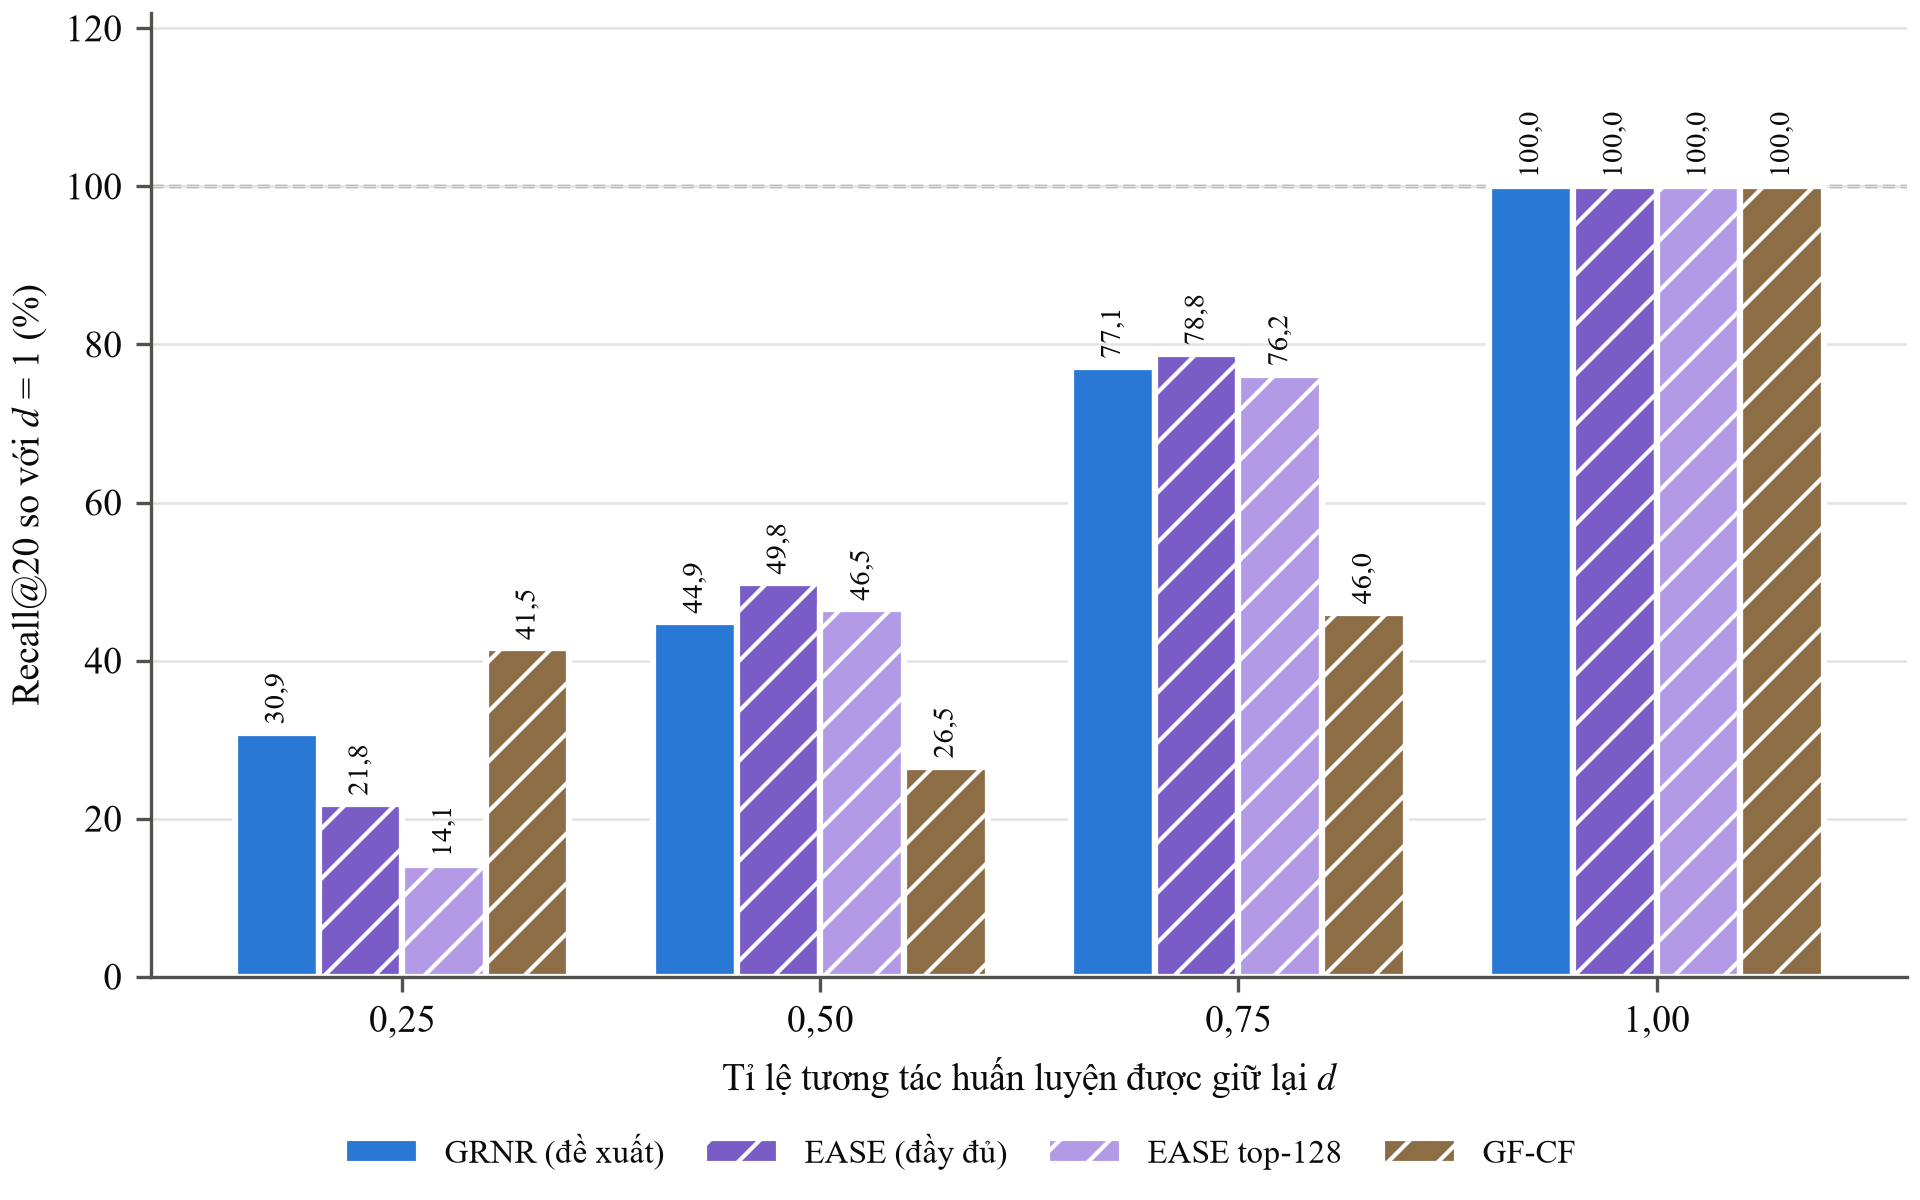
\includegraphics[width=0.75\linewidth]{H4_closed_form_retention_recall20.png}
\caption{Tỉ lệ duy trì Recall@20, nhóm giải trực tiếp}
\label{fig:closed-retention-recall20}
\end{figure}

\FloatBarrier
\subsubsection{Nguồn tín hiệu khi dữ liệu thưa}

Mức sụt so với MostPop có một nguyên nhân cơ học. Mọi mô hình trong nhóm đều học từ đồng xuất hiện, tức hai sản phẩm cùng nằm trong lịch sử của một người dùng, và một cặp chỉ còn khi cả hai tương tác cùng được giữ lại. Số cặp vì thế giảm nhanh hơn nhiều so với số tương tác. \Tabref{tab:cooccurrence} xác nhận điều đó: ở $d=0{,}25$, tập huấn luyện chỉ còn 4,2\% số cặp đồng xuất hiện. Trong bảng, số cặp theo người dùng là $\sum_u n_u(n_u-1)/2$, số cặp sản phẩm là số cặp sản phẩm khác nhau có $C_{ij}>0$, còn hai hàng cuối đếm hệ số láng giềng khác 0 trong checkpoint GRNR. Có thể đối chiếu với một mốc lý thuyết đơn giản: nếu mỗi tương tác được giữ độc lập với xác suất $d$, một cặp chỉ còn với xác suất $d^2$. Ở $d=0{,}75$ và $d=0{,}5$, số đo là 56,3\% và 24,2\%, gần sát mốc 56,25\% và 25\%; chỉ ở $d=0{,}25$, số đo 4,2\% thấp hơn rõ so với mốc 6,25\%. Một cách giải thích là cách giảm dữ liệu giữ ít nhất một tương tác cho mỗi người dùng (Mục~\ref{sec:sparsity-protocol}): khi dữ liệu còn rất ít, một phần đáng kể số tương tác được giữ lại dồn vào những người dùng chỉ còn một tương tác, vốn không tạo ra cặp nào. Ảnh hưởng lên GRNR thấy rõ qua số láng giềng: mỗi sản phẩm trung bình có 89,8 láng giềng ở $d=1$ nhưng chỉ còn 11,1 ở $d=0{,}25$, và 12,7\% sản phẩm không còn láng giềng nào. Với những sản phẩm này, điểm của GRNR chỉ còn hệ số chặn $b_i$, tức một dạng độ phổ biến.

\begin{table}[H]
\centering
\small
\begin{tabular}{@{}lrrrr@{}}
\toprule
& $d=1$ & $d=0{,}75$ & $d=0{,}5$ & $d=0{,}25$ \\
\midrule
Số tương tác & 100{,}0\% & 75{,}0\% & 50{,}0\% & 25{,}0\% \\
Số cặp đồng xuất hiện theo người dùng & 100{,}0\% & 56{,}3\% & 24{,}2\% & 4{,}2\% \\
Số cặp sản phẩm có đồng xuất hiện & 100{,}0\% & 58{,}5\% & 26{,}1\% & 4{,}7\% \\
\midrule
Số láng giềng trung bình của GRNR & 89{,}8 & 68{,}9 & 42{,}5 & 11{,}1 \\
Sản phẩm không có láng giềng & 0{,}1\% & 0{,}1\% & 0{,}8\% & 12{,}7\% \\
\bottomrule
\end{tabular}
\caption{Đồng xuất hiện còn lại trong tập huấn luyện}
\label{tab:cooccurrence}
\end{table}

NDCG@20 của GRNR giảm cùng chiều với số cặp đồng xuất hiện nhưng chậm hơn nhiều: ở mức thưa nhất, số cặp chỉ còn 4,2\% còn NDCG@20 vẫn giữ 24,7\%. Một phần chênh lệch này đến từ hệ số chặn, vốn không cần đồng xuất hiện. GRNR cũng là mô hình ít tệ nhất trong nhóm ở mức thưa nhất, kém MostPop 59\% so với 67\% của EASE đầy đủ. Vì bài toán của GRNR neo hệ số chặn vào xác suất nền của sản phẩm và phạt nặng các láng giềng ít dữ liệu, có thể khi thiếu đồng xuất hiện, mô hình dựa nhiều hơn vào hệ số chặn thay vì các hệ số nhiễu. Đây mới là giả thuyết, và phân tích độ phổ biến dưới đây không ủng hộ nó.

Nếu GRNR thật sự xếp hạng gần theo độ phổ biến khi dữ liệu thưa, các sản phẩm được gợi ý phải phổ biến hơn và tập trung vào ít sản phẩm hơn. \Tabref{tab:closed-popularity}, tính theo Mục~\ref{sec:beyond-accuracy}, cho thấy điều ngược lại. Độ phổ biến trung bình sau biến đổi log của GRNR giảm từ 5,60 ở $d=1$ xuống 4,18 ở $d=0{,}5$ và chỉ nhích lên 4,50 ở mức thưa nhất; hai biến thể EASE thì giảm đều. Khi đồng xuất hiện cạn, cả nhóm gợi ý những sản phẩm ít phổ biến hơn chứ không lùi về sản phẩm phổ biến. Một giải thích khác phù hợp hơn với số liệu: hệ số láng giềng của các sản phẩm ít tương tác trở nên nhiễu và đẩy chính các sản phẩm này lên danh sách.

Độ phủ danh mục trong top-20, tính trên 44.803 sản phẩm của tập huấn luyện gốc, cùng chiều với nhận xét này: GRNR gợi ý ít nhất một lần khoảng 85\% danh mục ở cả $d=1$ lẫn $d=0{,}25$, tức danh sách không co lại về một nhóm nhỏ sản phẩm. GF-CF có độ phủ trên 93\% ở mọi mức dù xếp hạng kém, cho thấy độ phủ cao chỉ nói rằng nhiều sản phẩm xuất hiện trong danh sách, chưa nói gì về việc chúng có hợp với người nhận hay không.

\begin{table}[H]
\centering
\small
\begin{tabular}{@{}lrrrr@{}}
\toprule
& $d=1$ & $d=0{,}75$ & $d=0{,}5$ & $d=0{,}25$ \\
\midrule
\multicolumn{5}{@{}l}{Độ phổ biến trung bình (log)} \\
GRNR & 5{,}60 & 5{,}02 & 4{,}18 & 4{,}50 \\
EASE đầy đủ & 5{,}64 & 5{,}39 & 4{,}85 & 4{,}25 \\
EASE top-128 & 5{,}12 & 4{,}89 & 4{,}42 & 3{,}38 \\
GF-CF & 2{,}68 & 2{,}38 & 2{,}58 & 3{,}68 \\
\midrule
\multicolumn{5}{@{}l}{Độ phủ danh mục trong top-20 (\%)} \\
GRNR & 85{,}4 & 94{,}9 & 97{,}6 & 84{,}7 \\
EASE đầy đủ & 72{,}3 & 92{,}8 & 96{,}3 & 83{,}7 \\
EASE top-128 & 87{,}0 & 95{,}9 & 97{,}0 & 84{,}2 \\
GF-CF & 98{,}6 & 99{,}4 & 99{,}9 & 93{,}9 \\
\bottomrule
\end{tabular}
\caption{Độ phổ biến và độ phủ, nhóm giải trực tiếp}
\label{tab:closed-popularity}
\end{table}

\FloatBarrier
\subsubsection{Chất lượng theo độ dài lịch sử người dùng}

Một cách khác để đọc kết quả là chia người dùng theo số tương tác trong tập huấn luyện gốc thành ba nhóm: 3--4, 5--9 và từ 10 tương tác trở lên, lần lượt có 54.693, 36.673 và 15.721 người dùng. \Figref{fig:closed-groups} cho một kết quả ngược trực giác: khi có đủ dữ liệu, người dùng có nhiều tương tác hơn lại được gợi ý kém hơn. Ở $d=1$, NDCG@20 của GRNR giảm từ 0,0298 ở nhóm ngắn nhất xuống 0,0227 ở nhóm dài nhất, và hai biến thể EASE cũng vậy. Có hai cách giải thích mà báo cáo chưa kiểm tra: người dùng nhiều tương tác có thể có sở thích trải rộng hơn, nên lịch sử ít định hướng cho lần mua tiếp theo; hoặc sản phẩm mục tiêu của họ ít phổ biến hơn và khó đoán với mọi mô hình. Hiện tượng này lặp lại ở nhóm cần huấn luyện, nên nhiều khả năng đây là tính chất của dữ liệu hơn là của riêng một mô hình. Tuy vậy, nó không đúng ở mọi mức: ở $d=0{,}5$, chiều này đảo lại, với GRNR đạt 0,0118 ở nhóm ngắn nhất nhưng 0,0147 ở nhóm dài nhất.

Cách chia này cũng cho biết ưu thế của GRNR ở mức thưa nhất đến từ đâu. GRNR hơn EASE đầy đủ ở hai nhóm lịch sử ngắn, chẳng hạn 0,0079 so với 0,0057 ở nhóm 3--4, nhưng kém ở nhóm dài nhất, 0,0041 so với 0,0053. Ưu thế trung bình vì thế đến từ những người dùng ít tương tác, cũng là nhóm đông nhất. Các nhóm được cố định theo lịch sử gốc nên không đổi khi bớt dữ liệu, và các giá trị theo nhóm chỉ mang tính mô tả.

\begin{figure}[H]
\centering
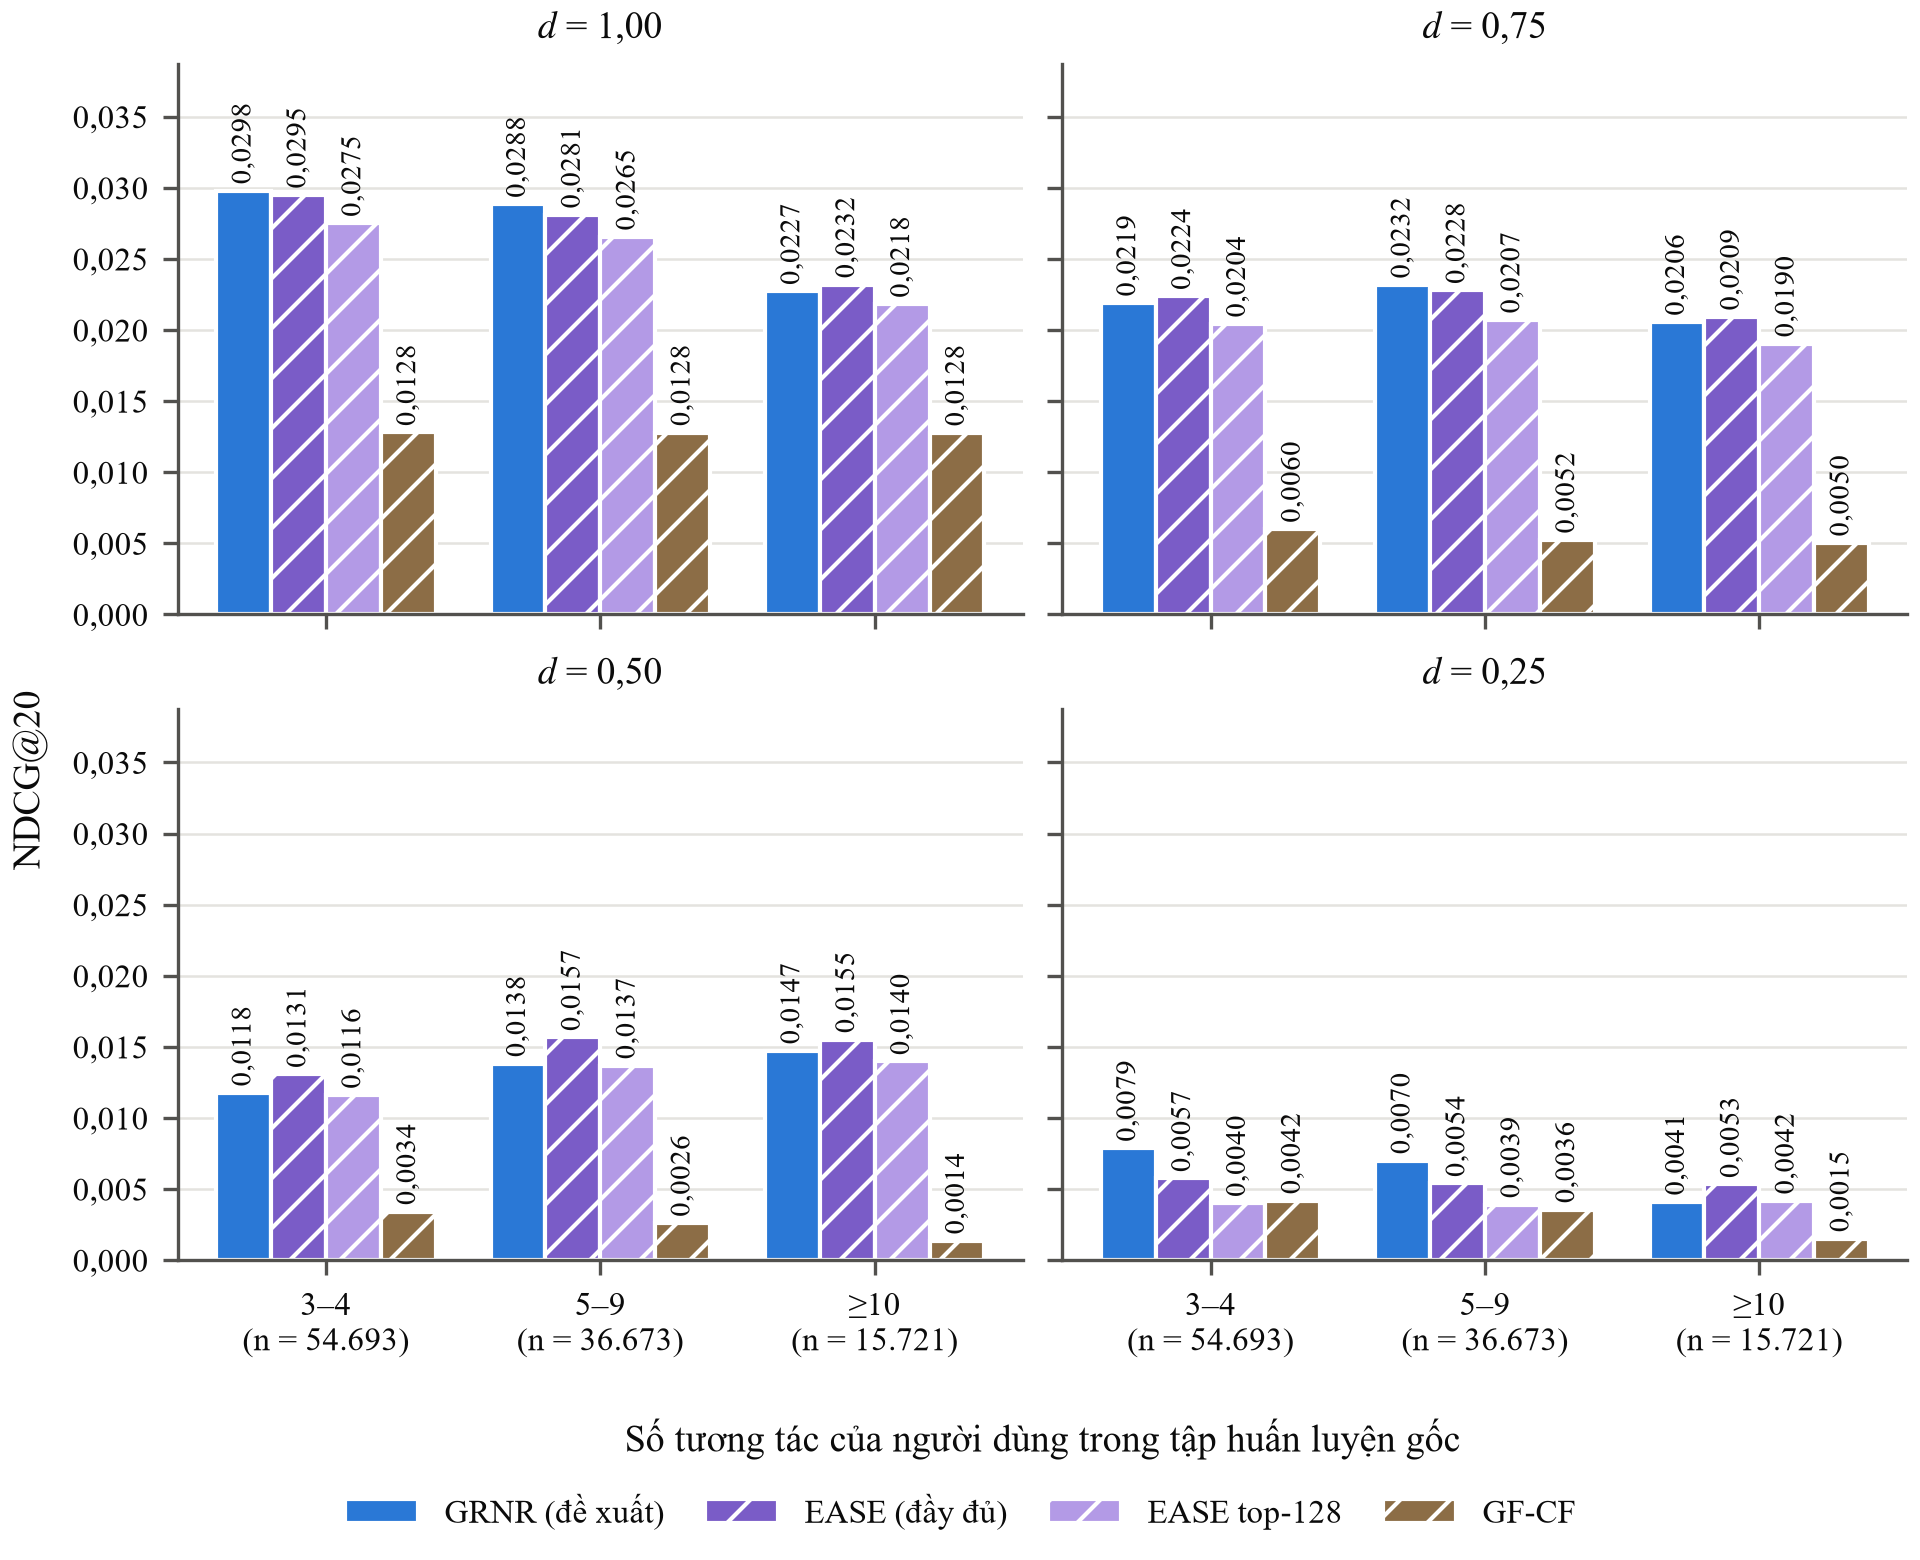
\includegraphics[width=0.68\linewidth]{H5_closed_form_user_groups_ndcg20.png}
\caption{NDCG@20 theo độ dài lịch sử, nhóm giải trực tiếp}
\label{fig:closed-groups}
\end{figure}

Thu hẹp về mười vị trí đầu như ở \figref{fig:closed-groups-ndcg10}, GRNR không còn dẫn ở mọi nhóm. Ngay ở $d=1$, GRNR chỉ cao nhất ở hai nhóm lịch sử ngắn, còn ở nhóm dài nhất EASE đầy đủ cao hơn, 0,0190 so với 0,0181. Sự phân hóa rõ nhất ở mức thưa nhất: GRNR hơn EASE đầy đủ ở nhóm 3--4, 0,0055 so với 0,0043, nhưng kém ở nhóm dài nhất, 0,0031 so với 0,0044. Mức chênh trung bình giữa hai mô hình vì vậy che đi hai chiều ngược nhau giữa các nhóm người dùng.

\begin{figure}[H]
\centering
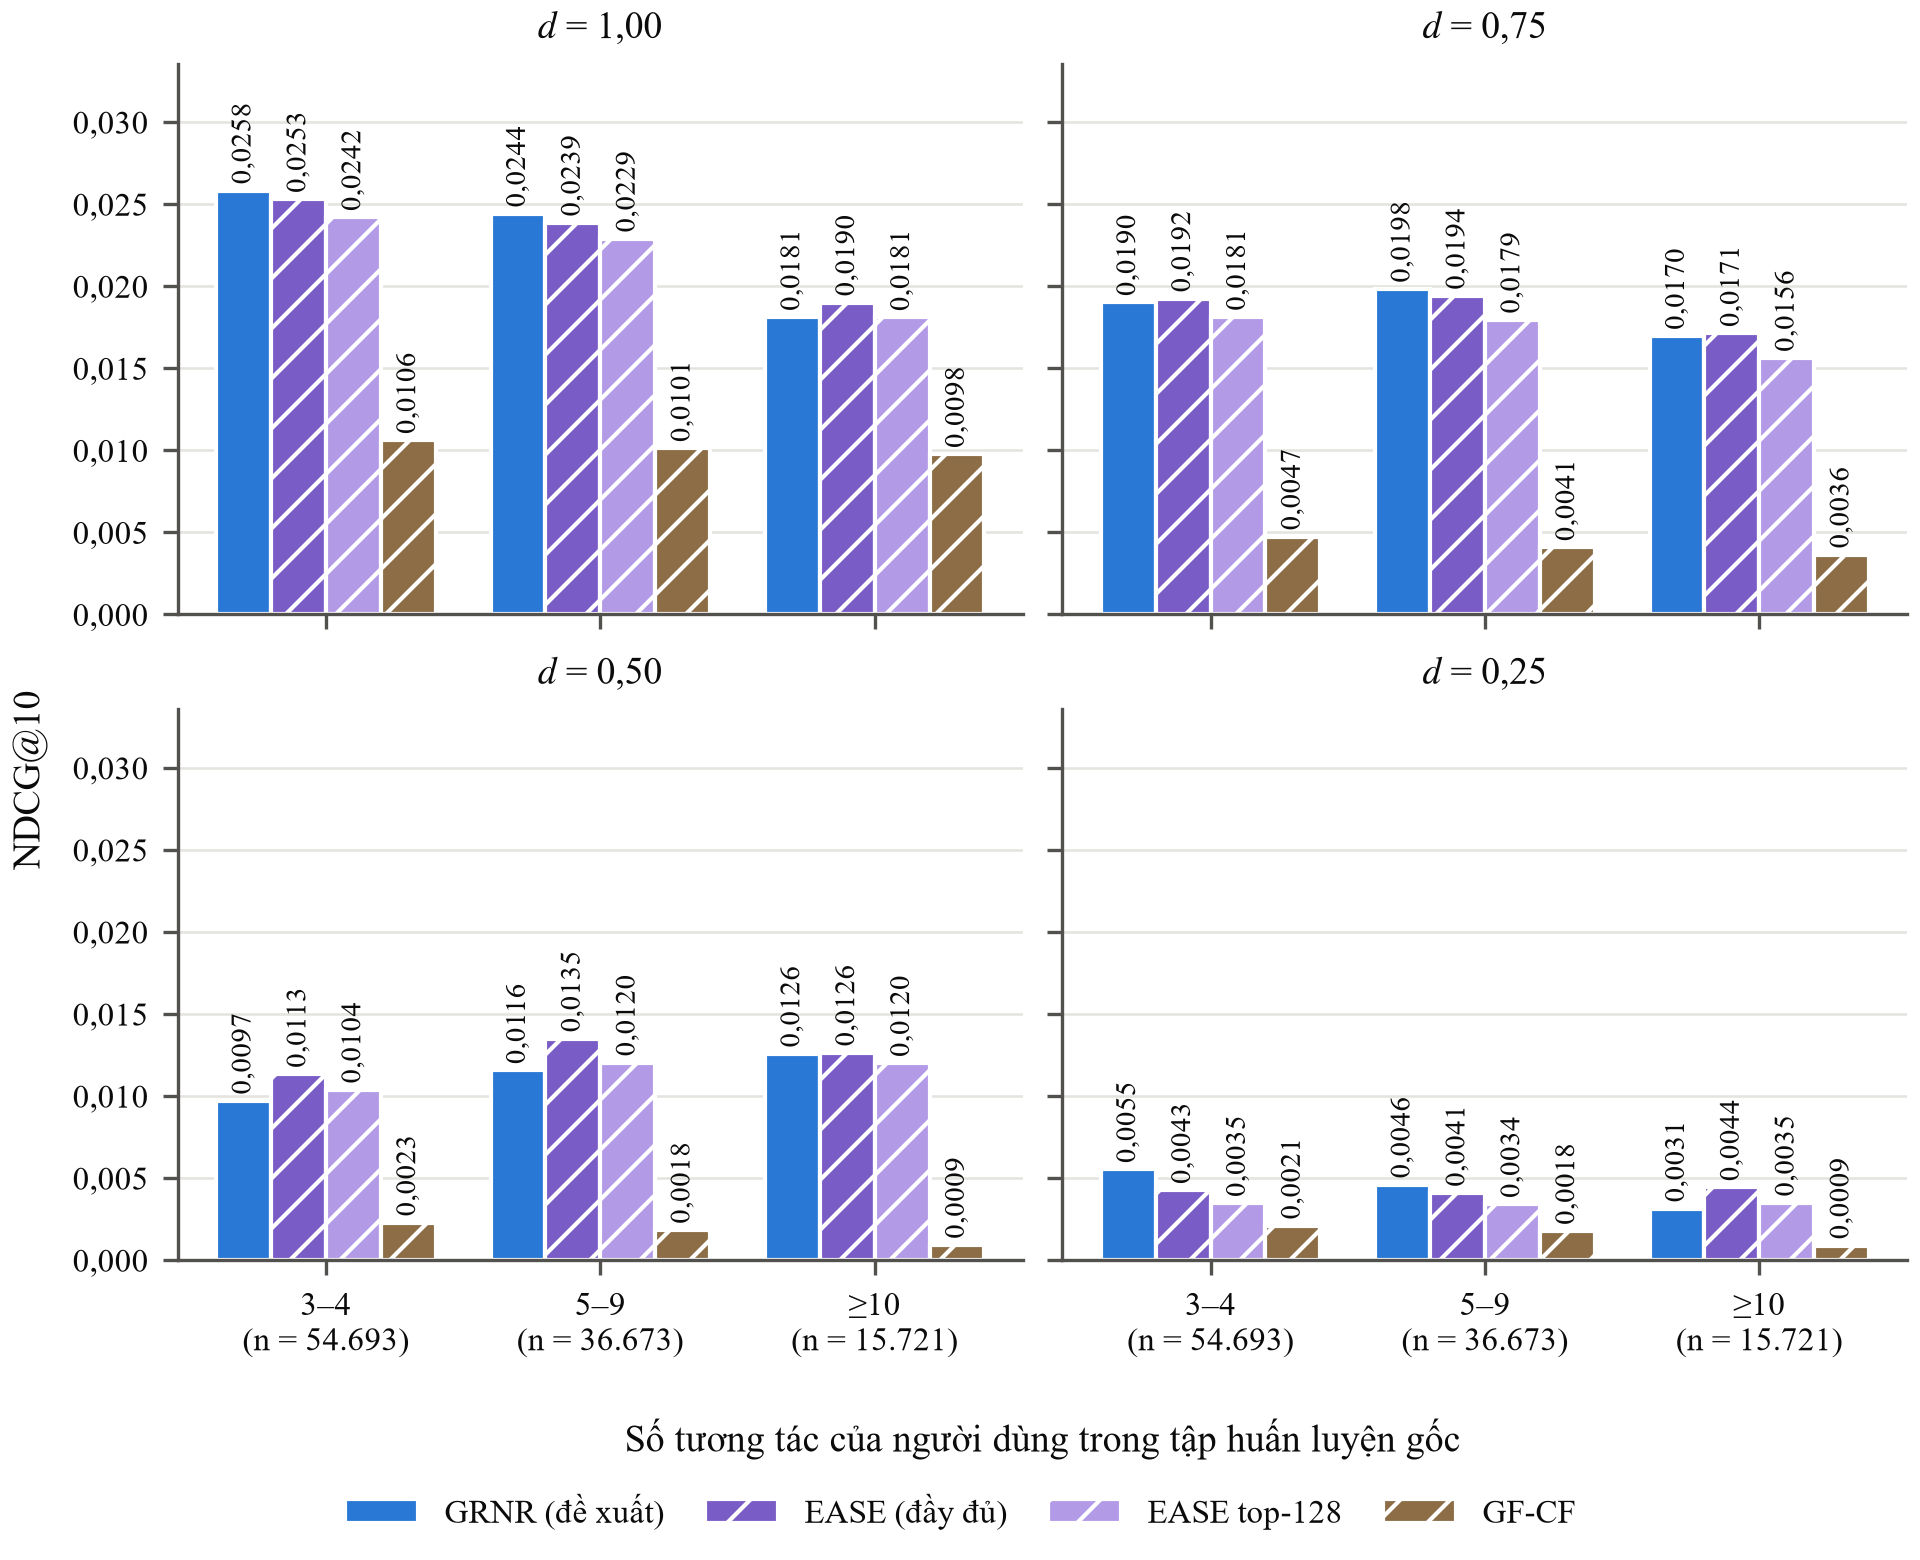
\includegraphics[width=0.68\linewidth]{H5_closed_form_user_groups_ndcg10.png}
\caption{NDCG@10 theo độ dài lịch sử, nhóm giải trực tiếp}
\label{fig:closed-groups-ndcg10}
\end{figure}

Recall@10 ở \figref{fig:closed-groups-recall10} cho thấy rõ hơn rằng nhận xét ``lịch sử dài thì khó gợi ý hơn'' phụ thuộc vào lượng dữ liệu. Ở $d=1$, Recall@10 của GRNR giảm đều theo độ dài lịch sử, từ 0,0449 xuống 0,0338. Nhưng ở $d=0{,}5$, nhóm dài nhất lại có Recall@10 cao nhất, 0,0223 so với 0,0162 ở nhóm ngắn nhất, và EASE đầy đủ cũng đảo chiều tương tự. Có thể là sau khi bớt dữ liệu, người dùng lịch sử dài vẫn còn vài tương tác để tạo đồng xuất hiện, trong khi nhiều người dùng lịch sử ngắn chỉ còn một; báo cáo chưa kiểm tra giải thích này. Ở mức thưa nhất, mẫu hình của NDCG@10 quay lại: GRNR dẫn ở hai nhóm ngắn nhưng thua EASE đầy đủ ở nhóm dài nhất.

\begin{figure}[H]
\centering
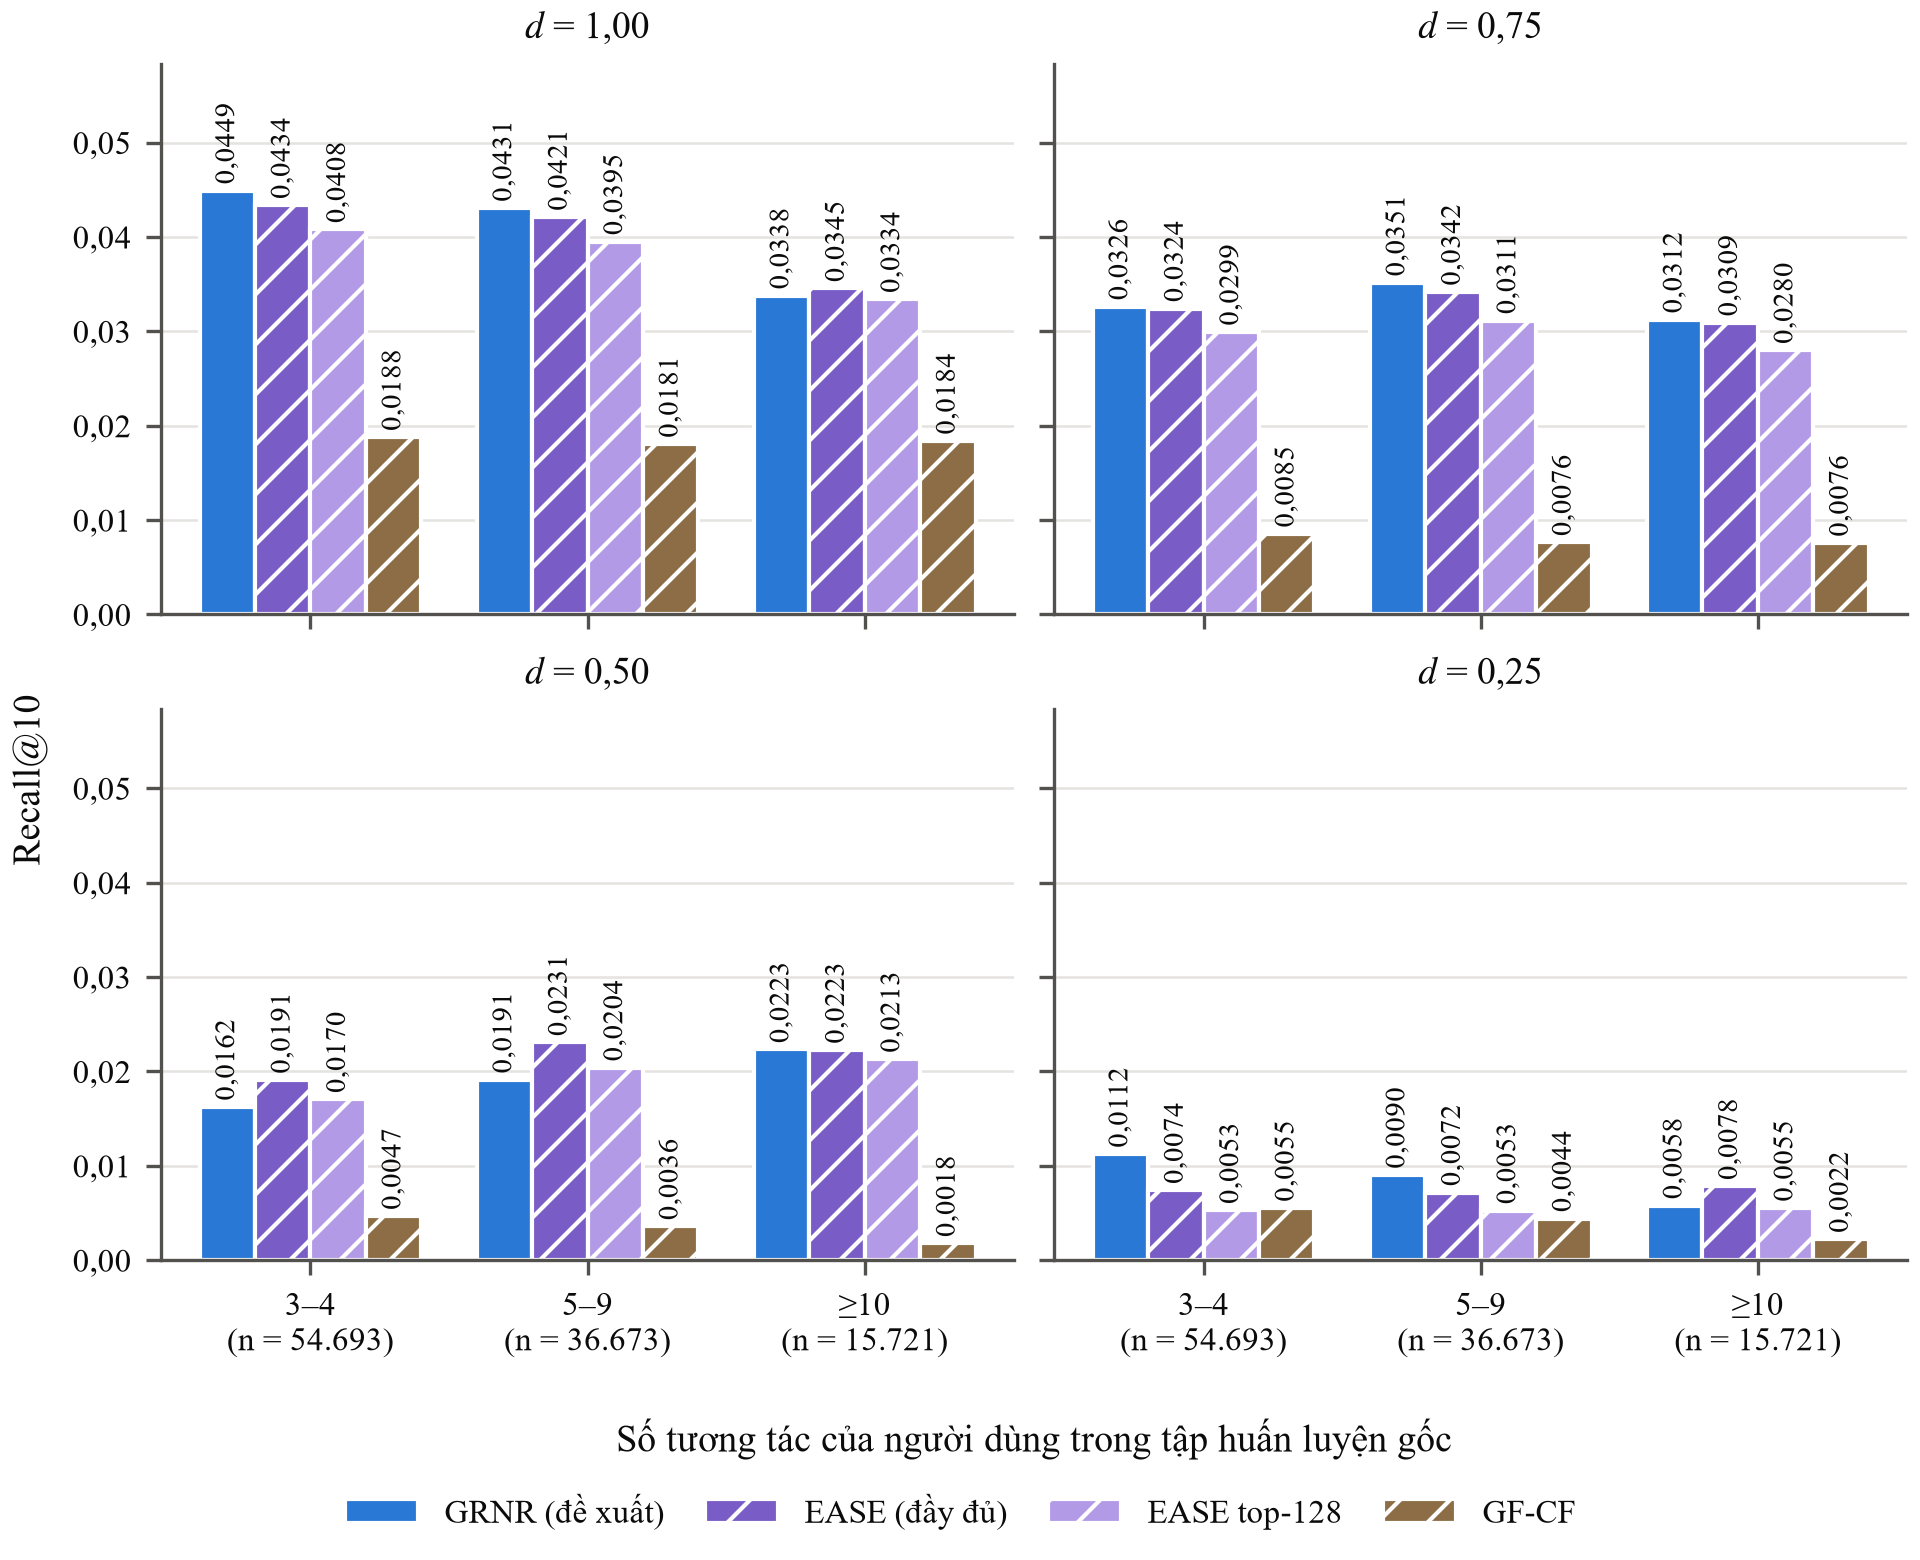
\includegraphics[width=0.68\linewidth]{H5_closed_form_user_groups_recall10.png}
\caption{Recall@10 theo độ dài lịch sử, nhóm giải trực tiếp}
\label{fig:closed-groups-recall10}
\end{figure}

Recall@20 ở \figref{fig:closed-groups-recall20} cho sự đảo chiều ở $d=0{,}5$ rõ nhất: Recall@20 của EASE đầy đủ tăng dần theo độ dài lịch sử, từ 0,0260 lên 0,0336, ngược hẳn với ở $d=1$. Ở $d=0{,}75$, Recall@20 của GRNR gần như bằng nhau giữa ba nhóm. Nhận xét ``người dùng nhiều tương tác khó được gợi ý hơn'' vì thế chỉ đúng khi gắn với một thước đo và một mức dữ liệu cụ thể.

\begin{figure}[H]
\centering
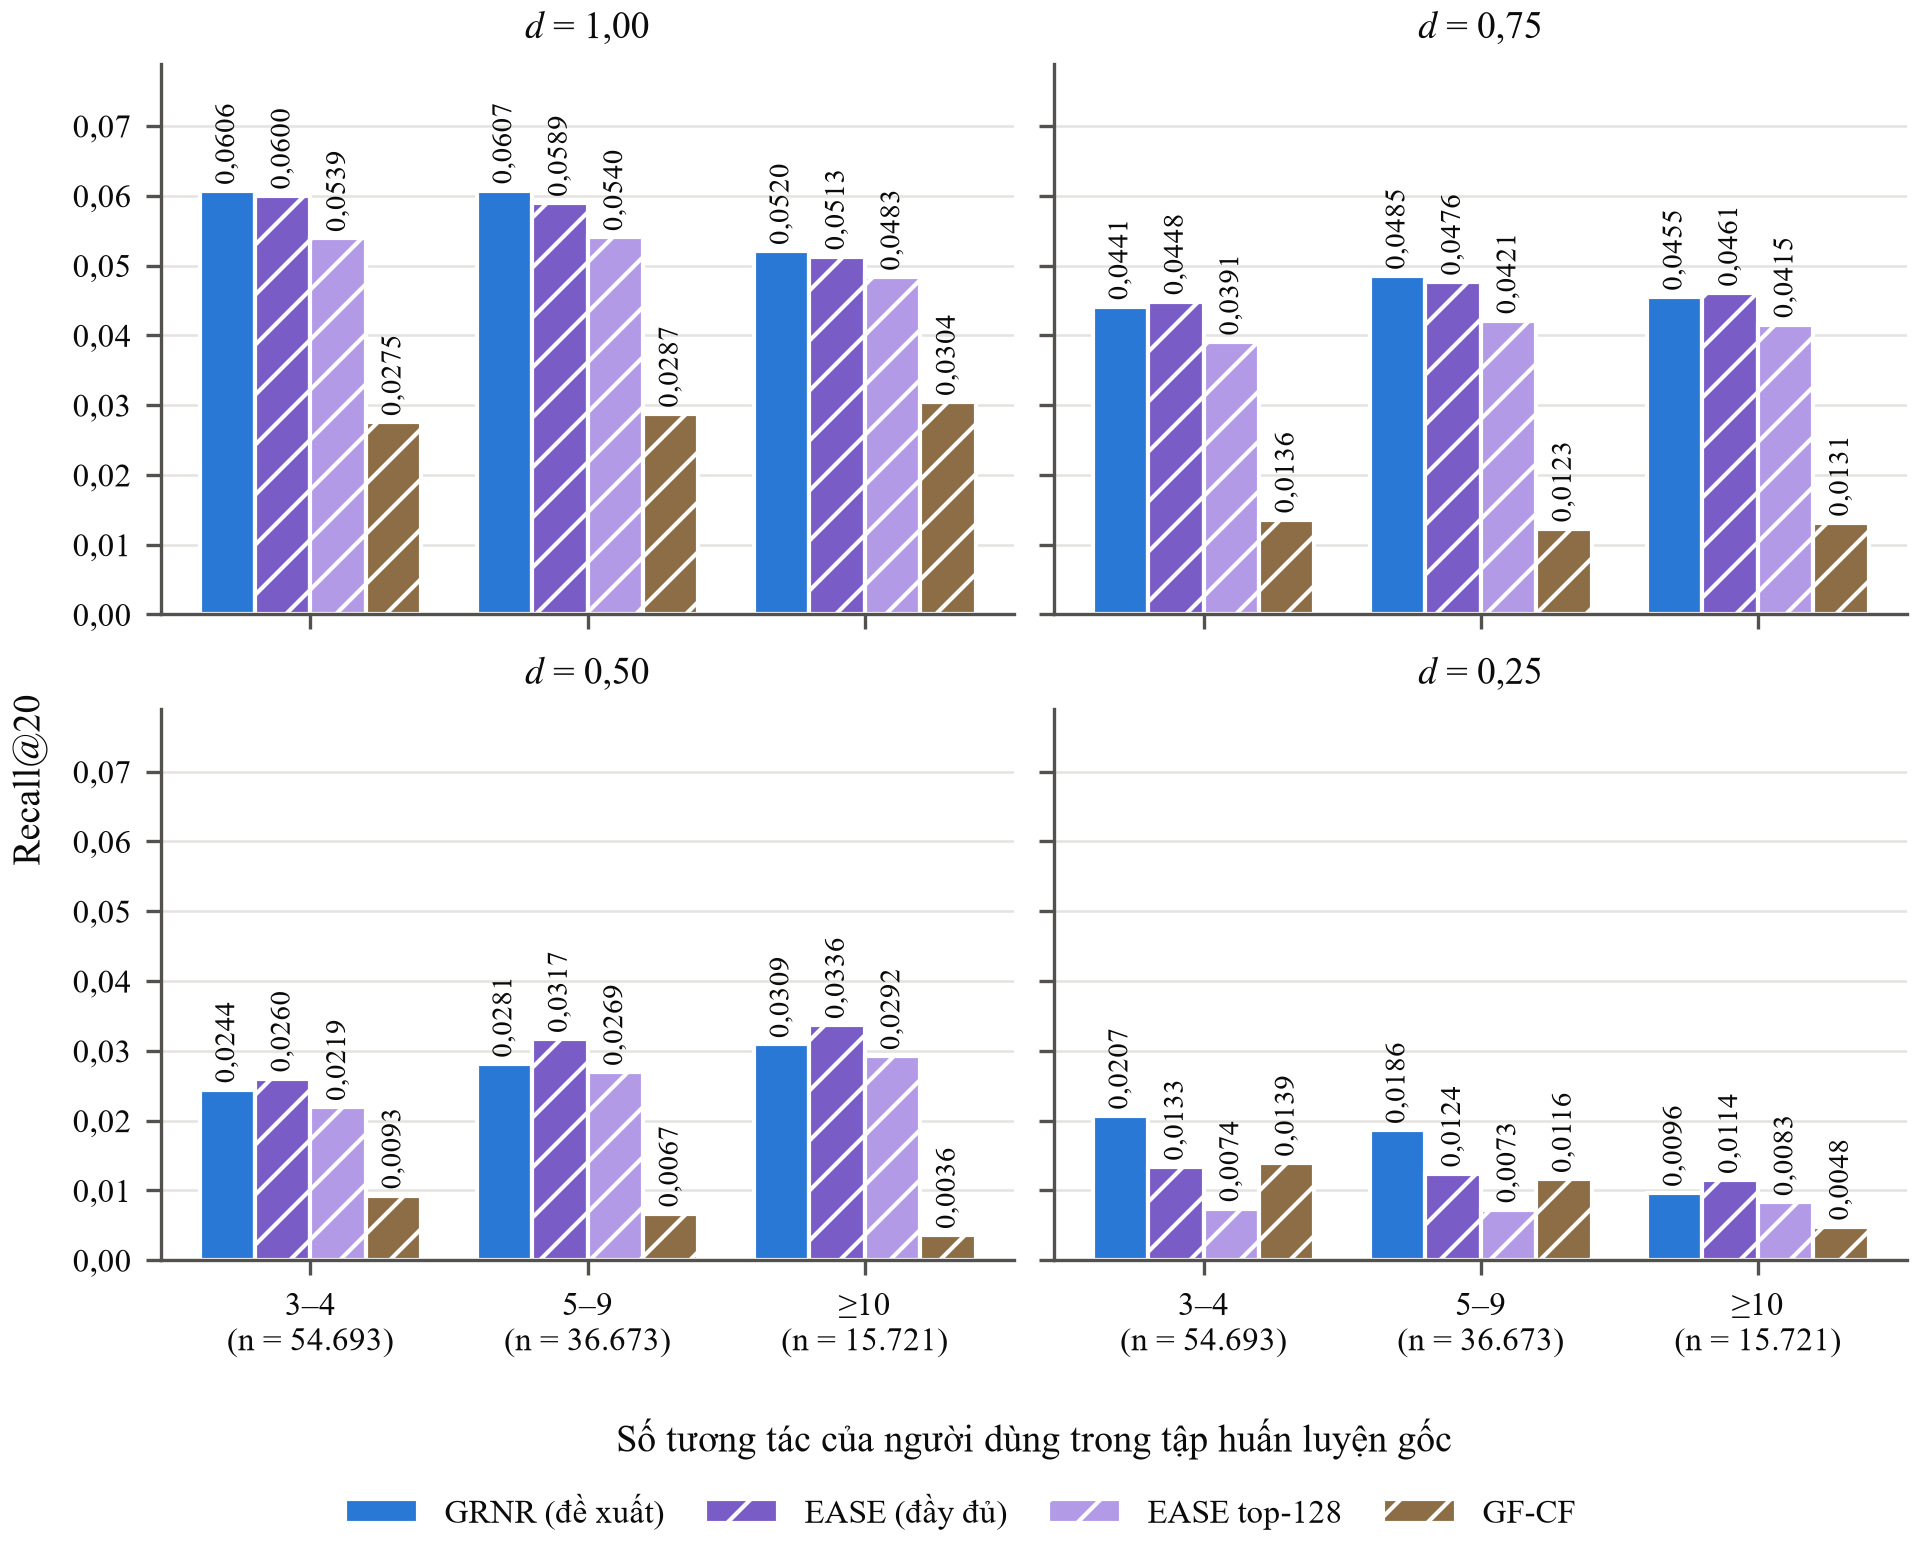
\includegraphics[width=0.68\linewidth]{H5_closed_form_user_groups_recall20.png}
\caption{Recall@20 theo độ dài lịch sử, nhóm giải trực tiếp}
\label{fig:closed-groups-recall20}
\end{figure}

\FloatBarrier
\subsubsection{Chi phí tính toán}

Về thời gian, ở $d=1$, GRNR mất 2,5 phút để khớp mô hình, EASE 11,2 phút và GF-CF 45,2 phút. Các con số này lẫn với khác biệt phần cứng, vì GRNR được giải trên CPU một luồng của máy có GPU còn EASE và GF-CF chạy trên máy chỉ có CPU; chúng mô tả chi phí trong môi trường của dự án, không phải tốc độ của bản thân thuật toán.

Dung lượng lưu trữ thì không phụ thuộc máy chạy, và \figref{fig:closed-size} cho thấy khoảng cách ở đây lên tới hai bậc. Ma trận đầy đủ của EASE ở dạng float32 chiếm khoảng 7.671 MiB, theo ước tính vì ma trận này không được lưu, gấp khoảng 190 lần checkpoint 40,5 MiB của GRNR. Khoảng cách này còn lớn dần theo quy mô danh mục: bộ nhớ của EASE tăng theo bình phương số sản phẩm, còn của GRNR tăng tuyến tính vì mỗi sản phẩm giữ tối đa 128 hệ số (Mục~\ref{sec:complexity}). Ngoại suy cho một danh mục lớn gấp 10 lần, EASE đầy đủ sẽ cần khoảng 750 GiB, trong khi GRNR chỉ cần khoảng 0,4 GiB. Cắt EASE xuống top-128 đưa dung lượng về cùng cỡ với GRNR, nhưng bản cắt kém GRNR ở cả bốn mức dữ liệu, rõ ràng ở ba mức, và kém EASE đầy đủ ở cả bốn mức. GF-CF vừa chậm nhất vừa yếu nhất nhóm, nên trong thiết lập này không có đánh đổi nào có lợi cho nó.

\begin{figure}[H]
\centering
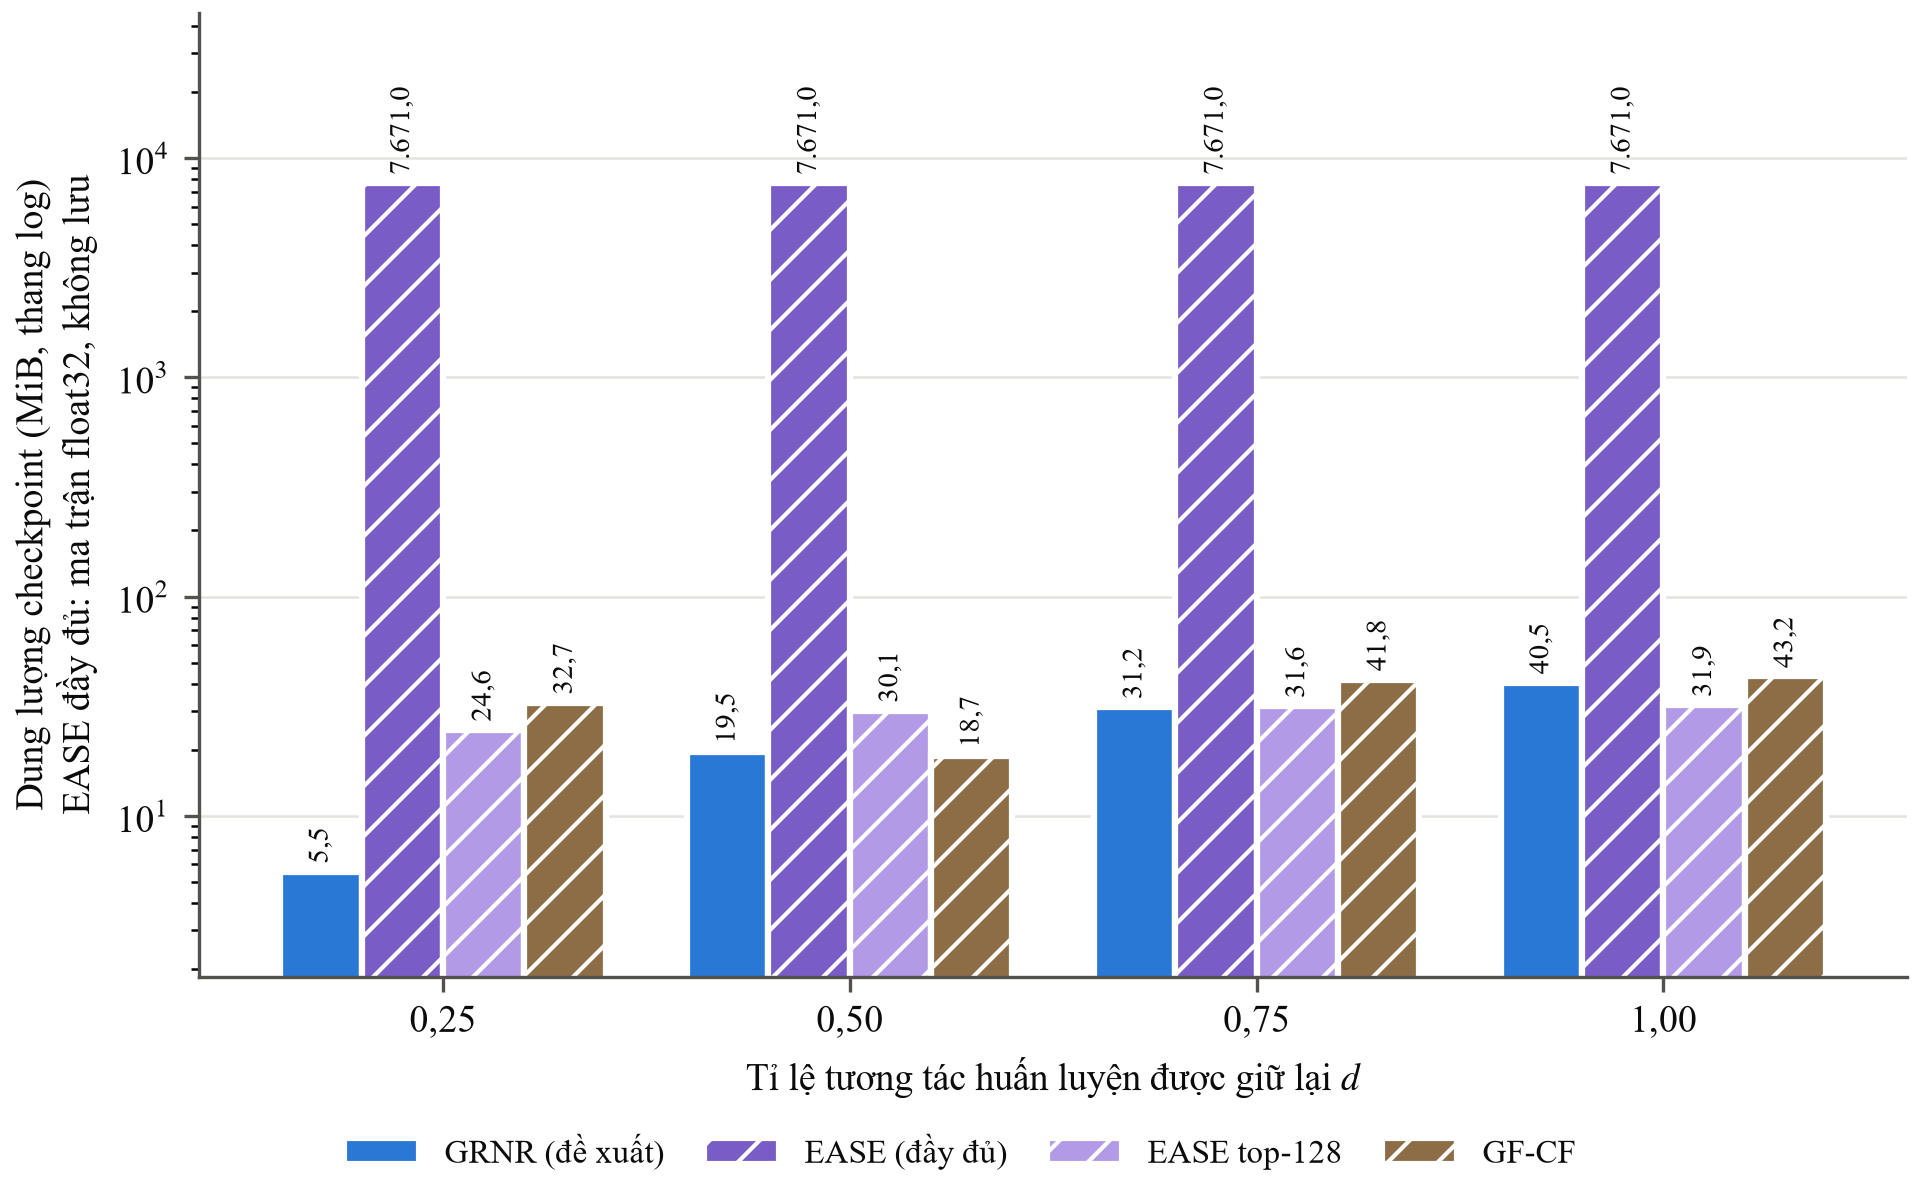
\includegraphics[width=0.75\linewidth]{H7c_closed_form_checkpoint_size.png}
\caption{Dung lượng lưu trữ, nhóm giải trực tiếp}
\label{fig:closed-size}
\end{figure}


Thời gian suy luận đã ghi lại của GRNR trên CPU là khoảng 0,38 ms mỗi người dùng ở $d=1$ và 0,88--0,90 ms ở ba mức còn lại, tức không giảm theo lượng dữ liệu. Đây là trung bình khi chấm điểm theo lô, chịu ảnh hưởng của cách thực thi và môi trường chạy; vì không có số đo cùng điều kiện cho EASE và GF-CF, báo cáo không kết luận về thứ tự tốc độ suy luận trong nhóm.

Tóm lại, khi dữ liệu còn dày, GRNR cho chất lượng chưa phân biệt được với EASE đầy đủ trong khi dung lượng nhỏ hơn hai bậc, và tốt hơn cách cắt EASE xuống cùng ngân sách. Khi dữ liệu thưa, ưu điểm này mất ý nghĩa: cả nhóm cùng cạn tín hiệu đồng xuất hiện và rơi xuống dưới mốc độ phổ biến ngay từ $d=0{,}5$, mức mà GRNR cũng thua EASE đầy đủ.

\FloatBarrier
\subsection{Diffusion-Filtered History Factorization so với các mô hình cần huấn luyện}
\label{sec:dfhf-results}

Ba baseline của nhóm này cùng dùng bộ mã hóa LightGCN, tức cùng một kiến trúc lan truyền trên đồ thị với vector riêng cho mỗi người dùng. Chúng chỉ khác nhau ở hàm mục tiêu: BPR (LightGCN), BPR cộng học tương phản (XSimGCL), và căn chỉnh--đồng đều (DirectAU). DFHF khác cả ba ở hai điểm cơ bản: không có vector người dùng, và huấn luyện bằng softmax trên toàn danh mục. Câu hỏi của mục này là các khác biệt đó đem lại gì, và mất gì.

\FloatBarrier
\subsubsection{Chất lượng xếp hạng khi có đủ dữ liệu}

Khi có đủ dữ liệu, DFHF dẫn đầu nhóm ở cả bốn thước đo trong \tabref{tab:trained}, với NDCG@20 bằng 0,02724.

\begin{table}[H]
\centering
\small
\begin{tabular}{@{}llrrrr@{}}
\toprule
$d$ & Mô hình & NDCG@10 & NDCG@20 & Recall@10 & Recall@20 \\
\midrule
\multirow{4}{*}{1} & DFHF & \textbf{0,02231} & \textbf{0,02724} & \textbf{0,04002} & \textbf{0,05966} \\
 & LightGCN & 0,01761 & 0,02168 & 0,03251 & 0,04870 \\
 & XSimGCL & 0,02107 & 0,02561 & 0,03843 & 0,05647 \\
 & DirectAU & 0,01991 & 0,02407 & 0,03599 & 0,05256 \\
\midrule
\multirow{4}{*}{0,75} & DFHF & \textbf{0,01889} & \textbf{0,02324} & \textbf{0,03436} & \textbf{0,05166} \\
 & LightGCN & 0,01534 & 0,01930 & 0,02878 & 0,04455 \\
 & XSimGCL & 0,01769 & 0,02158 & 0,03226 & 0,04773 \\
 & DirectAU & 0,01719 & 0,02065 & 0,03133 & 0,04503 \\
\midrule
\multirow{4}{*}{0,5} & DFHF & \textbf{0,01560} & \textbf{0,01971} & \textbf{0,02875} & \textbf{0,04510} \\
 & LightGCN & 0,01337 & 0,01691 & 0,02608 & 0,04020 \\
 & XSimGCL & 0,01269 & 0,01544 & 0,02281 & 0,03377 \\
 & DirectAU & 0,01308 & 0,01585 & 0,02333 & 0,03435 \\
\midrule
\multirow{4}{*}{0,25} & DFHF & \textbf{0,01315} & \textbf{0,01710} & \textbf{0,02467} & \textbf{0,04023} \\
 & LightGCN & 0,00631 & 0,00786 & 0,01193 & 0,01807 \\
 & XSimGCL & 0,00807 & 0,01019 & 0,01566 & 0,02408 \\
 & DirectAU & 0,00695 & 0,00856 & 0,01242 & 0,01884 \\
\bottomrule
\end{tabular}
\caption{Chất lượng xếp hạng, nhóm cần huấn luyện}
\label{tab:trained}
\end{table}

\Tabref{tab:trained-sig} cho thấy DFHF hơn XSimGCL 0,00163, hơn DirectAU 0,00317 và hơn LightGCN 0,00557, cả ba khoảng tin cậy đều nằm hẳn trên 0. Ưu thế này giữ nguyên ở cả bốn mức dữ liệu.

Thứ tự giữa các baseline cũng đáng chú ý. LightGCN, chỉ dùng BPR, yếu nhất nhóm; chỉ cần thay hàm mục tiêu và giữ nguyên bộ mã hóa, XSimGCL và DirectAU đã đạt 0,02561 và 0,02407, so với 0,02168 của LightGCN. Trong nhóm này, hàm mục tiêu như vậy có vẻ quan trọng hơn kiến trúc lan truyền. DFHF đi tiếp theo cùng hướng: softmax trên toàn danh mục so sánh sản phẩm dương với mọi sản phẩm cùng lúc thay vì với một mẫu âm ngẫu nhiên như BPR, nên gần với thước đo xếp hạng hơn~\cite{liang2018multvae}. Đây là cách giải thích phù hợp với dữ liệu nhưng chưa được kiểm chứng, vì báo cáo chưa có thí nghiệm tách đóng góp của hàm mất mát, bộ lọc khuếch tán và cách biểu diễn bằng lịch sử.

\begin{table}[H]
\centering
\small
\begin{tabular}{@{}llrcr@{}}
\toprule
$d$ & So sánh & $\Delta$ NDCG@20 & KTC 95\% & $p_{\mathrm{Holm}}$ (một phía) \\
\midrule
\multirow{3}{*}{1} & DFHF $-$ LightGCN & $+0{,}00557$ & $[+0{,}00502;\;+0{,}00610]$ & $\le 3\cdot10^{-4}$ \\
 & DFHF $-$ XSimGCL & $+0{,}00163$ & $[+0{,}00111;\;+0{,}00213]$ & $\le 3\cdot10^{-4}$ \\
 & DFHF $-$ DirectAU & $+0{,}00317$ & $[+0{,}00260;\;+0{,}00375]$ & $\le 3\cdot10^{-4}$ \\
\midrule
\multirow{3}{*}{0,75} & DFHF $-$ LightGCN & $+0{,}00394$ & $[+0{,}00342;\;+0{,}00448]$ & $\le 3\cdot10^{-4}$ \\
 & DFHF $-$ XSimGCL & $+0{,}00166$ & $[+0{,}00113;\;+0{,}00218]$ & $\le 3\cdot10^{-4}$ \\
 & DFHF $-$ DirectAU & $+0{,}00259$ & $[+0{,}00202;\;+0{,}00317]$ & $\le 3\cdot10^{-4}$ \\
\midrule
\multirow{3}{*}{0,5} & DFHF $-$ LightGCN & $+0{,}00280$ & $[+0{,}00232;\;+0{,}00328]$ & $\le 3\cdot10^{-4}$ \\
 & DFHF $-$ XSimGCL & $+0{,}00427$ & $[+0{,}00370;\;+0{,}00483]$ & $\le 3\cdot10^{-4}$ \\
 & DFHF $-$ DirectAU & $+0{,}00386$ & $[+0{,}00327;\;+0{,}00447]$ & $\le 3\cdot10^{-4}$ \\
\midrule
\multirow{3}{*}{0,25} & DFHF $-$ LightGCN & $+0{,}00924$ & $[+0{,}00867;\;+0{,}00981]$ & $\le 3\cdot10^{-4}$ \\
 & DFHF $-$ XSimGCL & $+0{,}00691$ & $[+0{,}00637;\;+0{,}00746]$ & $\le 3\cdot10^{-4}$ \\
 & DFHF $-$ DirectAU & $+0{,}00854$ & $[+0{,}00791;\;+0{,}00918]$ & $\le 3\cdot10^{-4}$ \\
\bottomrule
\end{tabular}
\caption{Kiểm định NDCG@20, nhóm cần huấn luyện}
\label{tab:trained-sig}
\end{table}

Số liệu của DirectAU trên tập kiểm tra cần được đọc cùng một lưu ý. Checkpoint được chọn trên tập xác thực của mô hình này rơi vào epoch cuối khi $d=1$, epoch 113 khi $d=0{,}75$, và epoch 195 và 181 ở hai mức còn lại. Nhiều khả năng DirectAU chưa hội tụ sau 200 epoch, nên các giá trị 0,02407 ở $d=1$ hay 0,00856 ở mức thưa nhất có thể thấp hơn mức mô hình đạt được nếu huấn luyện lâu hơn.

\FloatBarrier
\subsubsection{Chất lượng theo thước đo và độ dài danh sách}

\Figref{fig:trained-ndcg10} cho thấy DFHF giữ vị trí đầu ở mọi mức, nhưng khoảng cách với baseline mạnh nhất thay đổi theo $d$. Ở $d=1$ và $d=0{,}75$, DFHF hơn XSimGCL khoảng 0,0012. Ở $d=0{,}5$, đối thủ gần nhất đổi thành LightGCN và khoảng cách tăng lên 0,0022. Ở mức thưa nhất, khoảng cách lớn nhất, 0,0051, dù giá trị của cả nhóm khi đó đã thấp hơn nhiều. Một khoảng cách nới rộng đúng lúc dữ liệu cạn nhất là điều cần giải thích, chưa phải bằng chứng rằng DFHF học tốt hơn hẳn.

\begin{figure}[H]
\centering
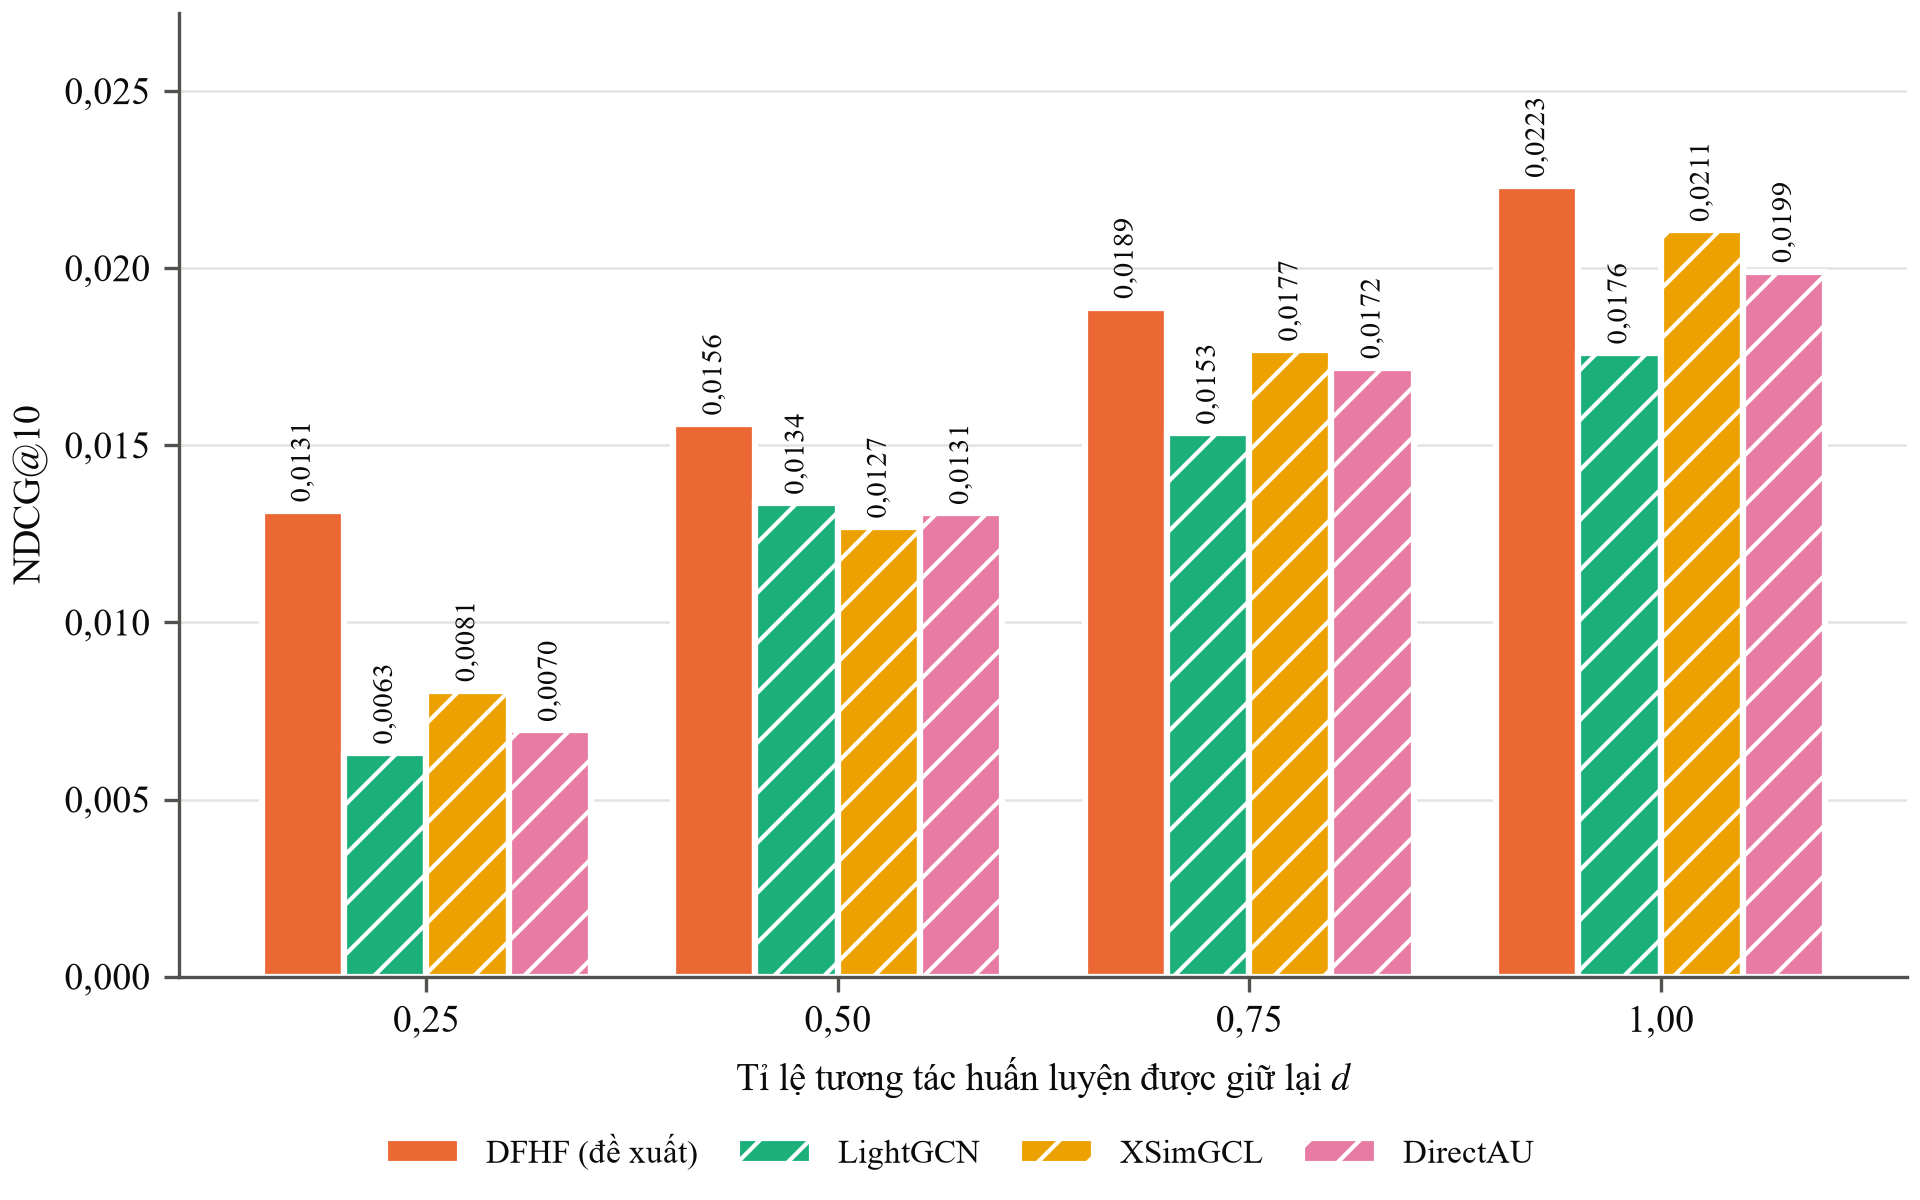
\includegraphics[width=0.75\linewidth]{H1_trained_density_ndcg10.png}
\caption{NDCG@10 theo mức $d$, nhóm cần huấn luyện}
\label{fig:trained-ndcg10}
\end{figure}

NDCG@20 ở \figref{fig:trained-ndcg20} giữ nguyên bức tranh đó: DFHF hơn baseline mạnh nhất khoảng 0,0016 khi $d\ge0{,}75$, 0,0028 ở $d=0{,}5$ và 0,0069 ở mức thưa nhất. Điều thay đổi theo $d$ là thứ tự giữa các baseline. LightGCN đứng cuối khi dữ liệu dày, vươn lên thứ hai ở $d=0{,}5$, rồi lại xuống cuối ở mức thưa nhất; XSimGCL đứng thứ hai ở ba mức còn lại. So sánh trên tập đầy đủ vì vậy chưa nói hết hành vi của các mô hình khi dữ liệu thưa.

\begin{figure}[H]
\centering
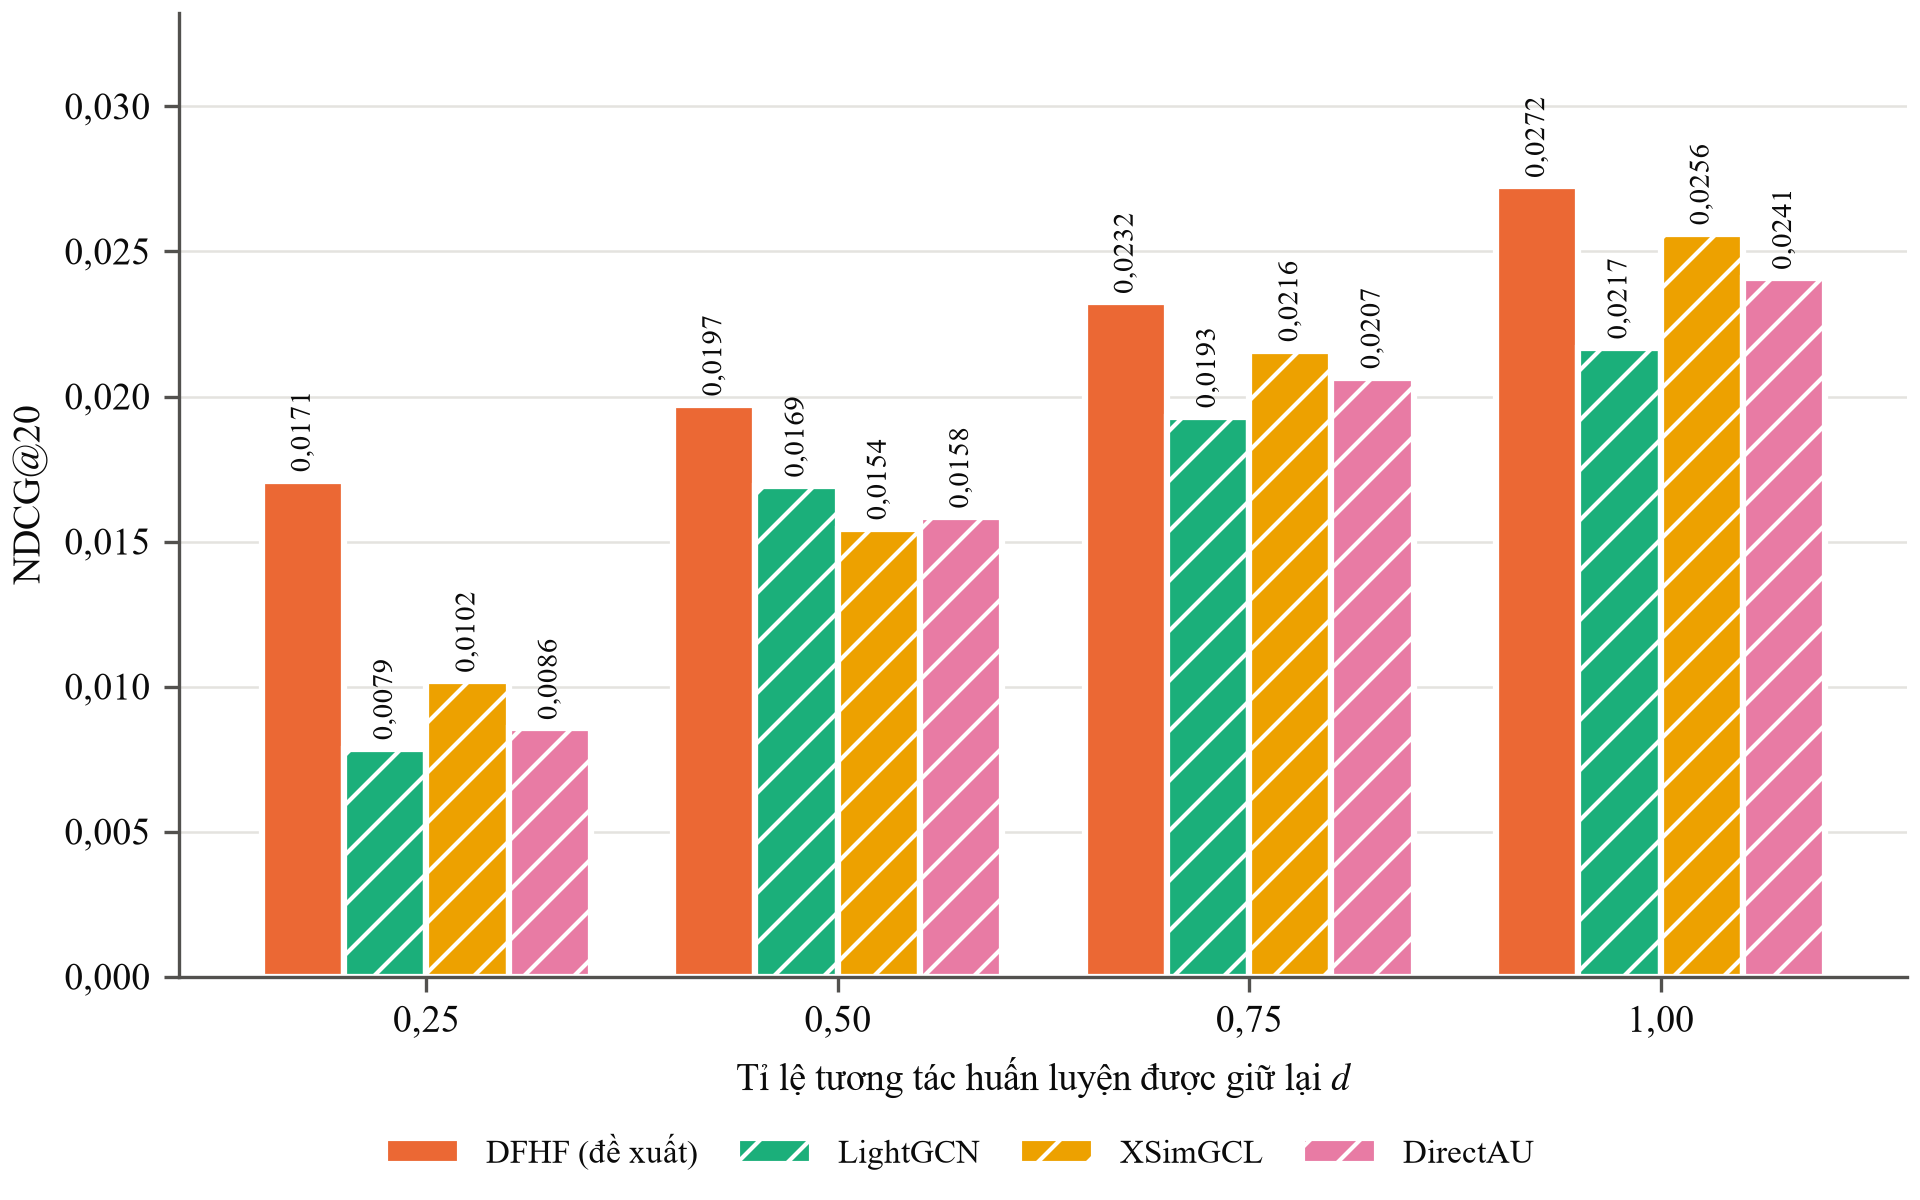
\includegraphics[width=0.75\linewidth]{H1_trained_density_ndcg20.png}
\caption{NDCG@20 theo mức $d$, nhóm cần huấn luyện}
\label{fig:trained-ndcg20}
\end{figure}

Recall@10 ở \figref{fig:trained-recall10} kể cùng câu chuyện: DFHF dẫn ở mọi mức, và khoảng cách tuyệt đối lớn nhất ở mức thưa nhất, nơi DFHF đạt 0,02467 còn XSimGCL chỉ đạt 0,01566.

\begin{figure}[H]
\centering
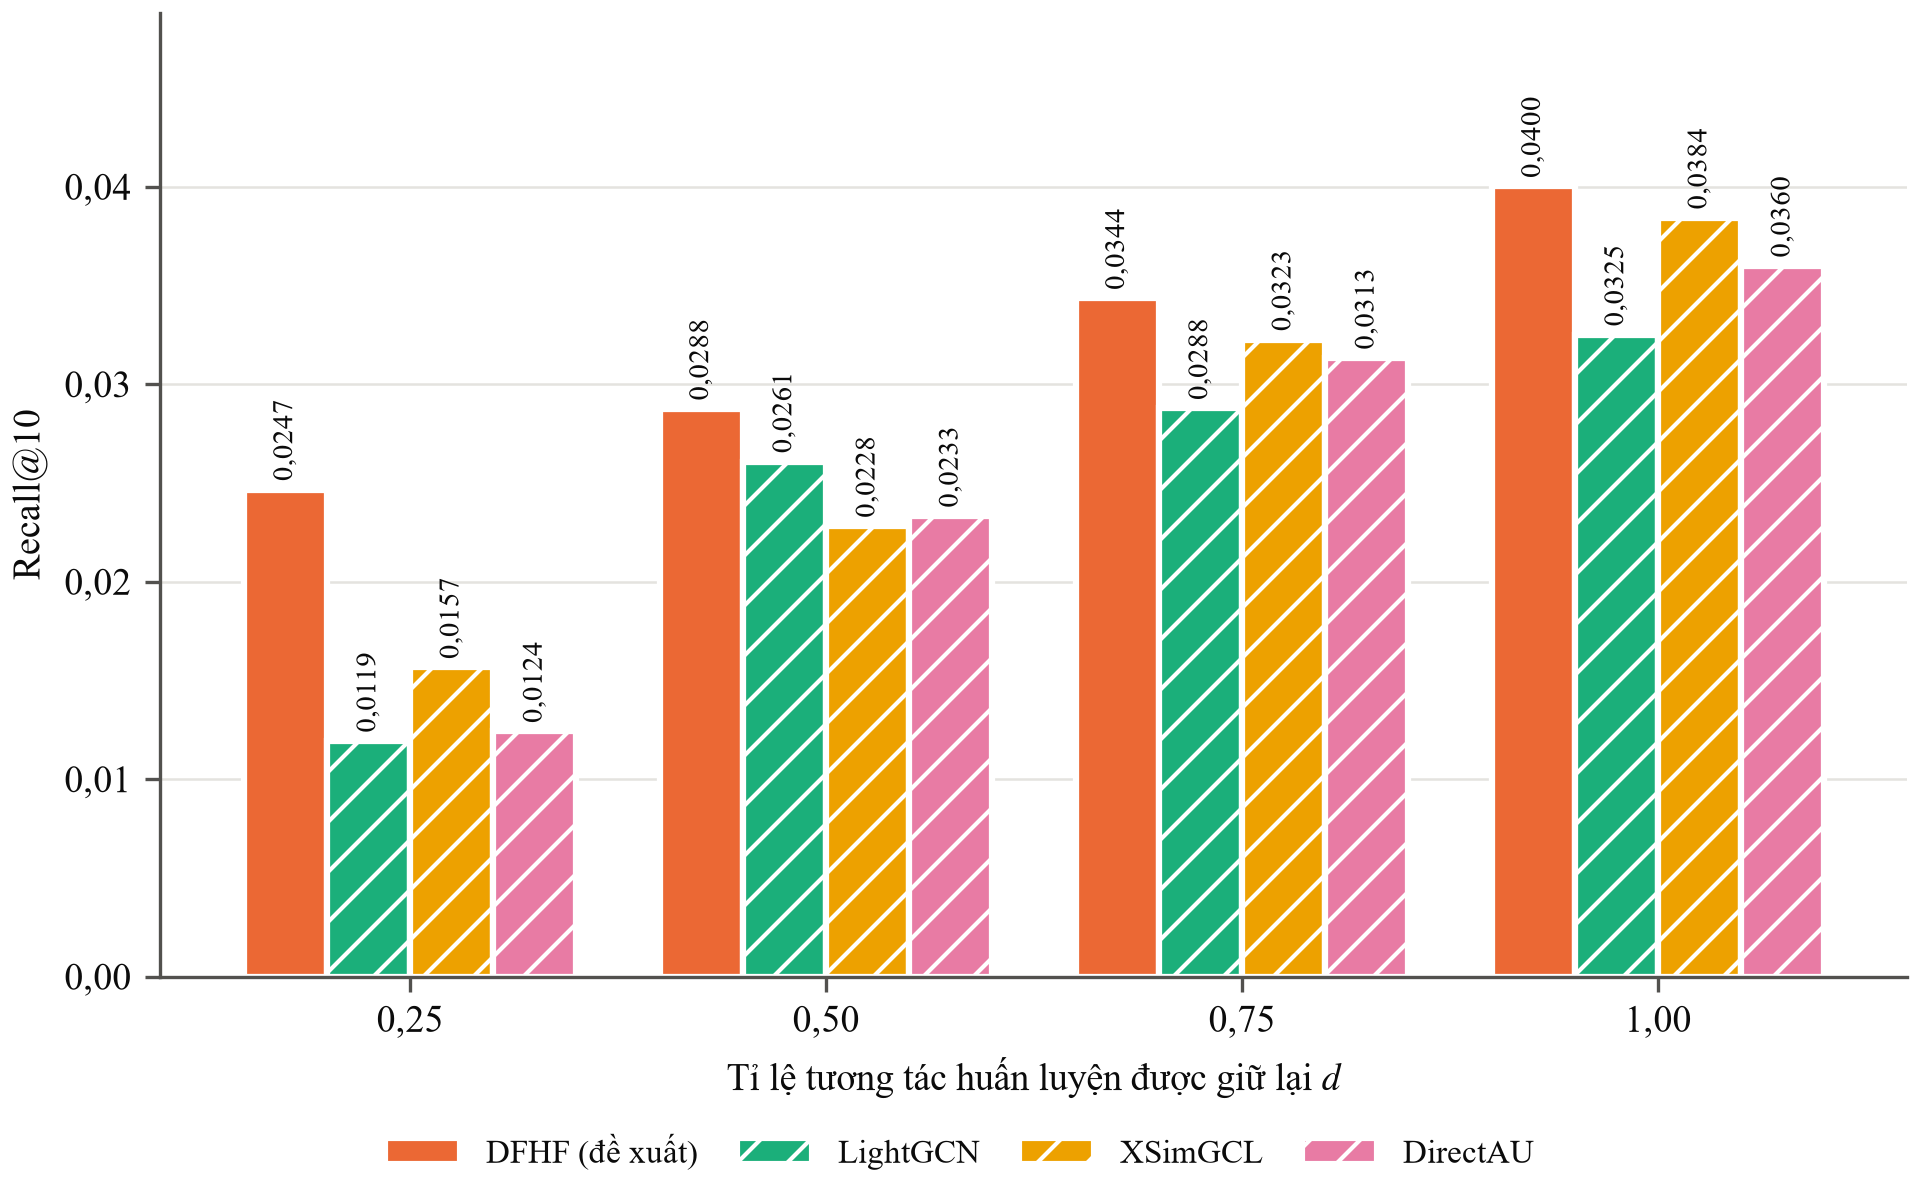
\includegraphics[width=0.75\linewidth]{H1_trained_density_recall10.png}
\caption{Recall@10 theo mức $d$, nhóm cần huấn luyện}
\label{fig:trained-recall10}
\end{figure}

Recall@20 ở \figref{fig:trained-recall20} cho cùng xu hướng, với khoảng cách giữa DFHF và XSimGCL tăng từ 0,0032 khi có đủ dữ liệu lên 0,0162 ở mức thưa nhất. Hình này cũng cho thấy rõ vị trí bất thường của LightGCN ở $d=0{,}5$: với Recall@20 bằng 0,04020, nó vượt cả XSimGCL lẫn DirectAU. Đây là mức duy nhất LightGCN không đứng cuối, và điều đó đúng ở cả bốn thước đo, nên thứ tự giữa các baseline phụ thuộc vào lượng dữ liệu nhiều hơn vào thước đo.

\begin{figure}[H]
\centering
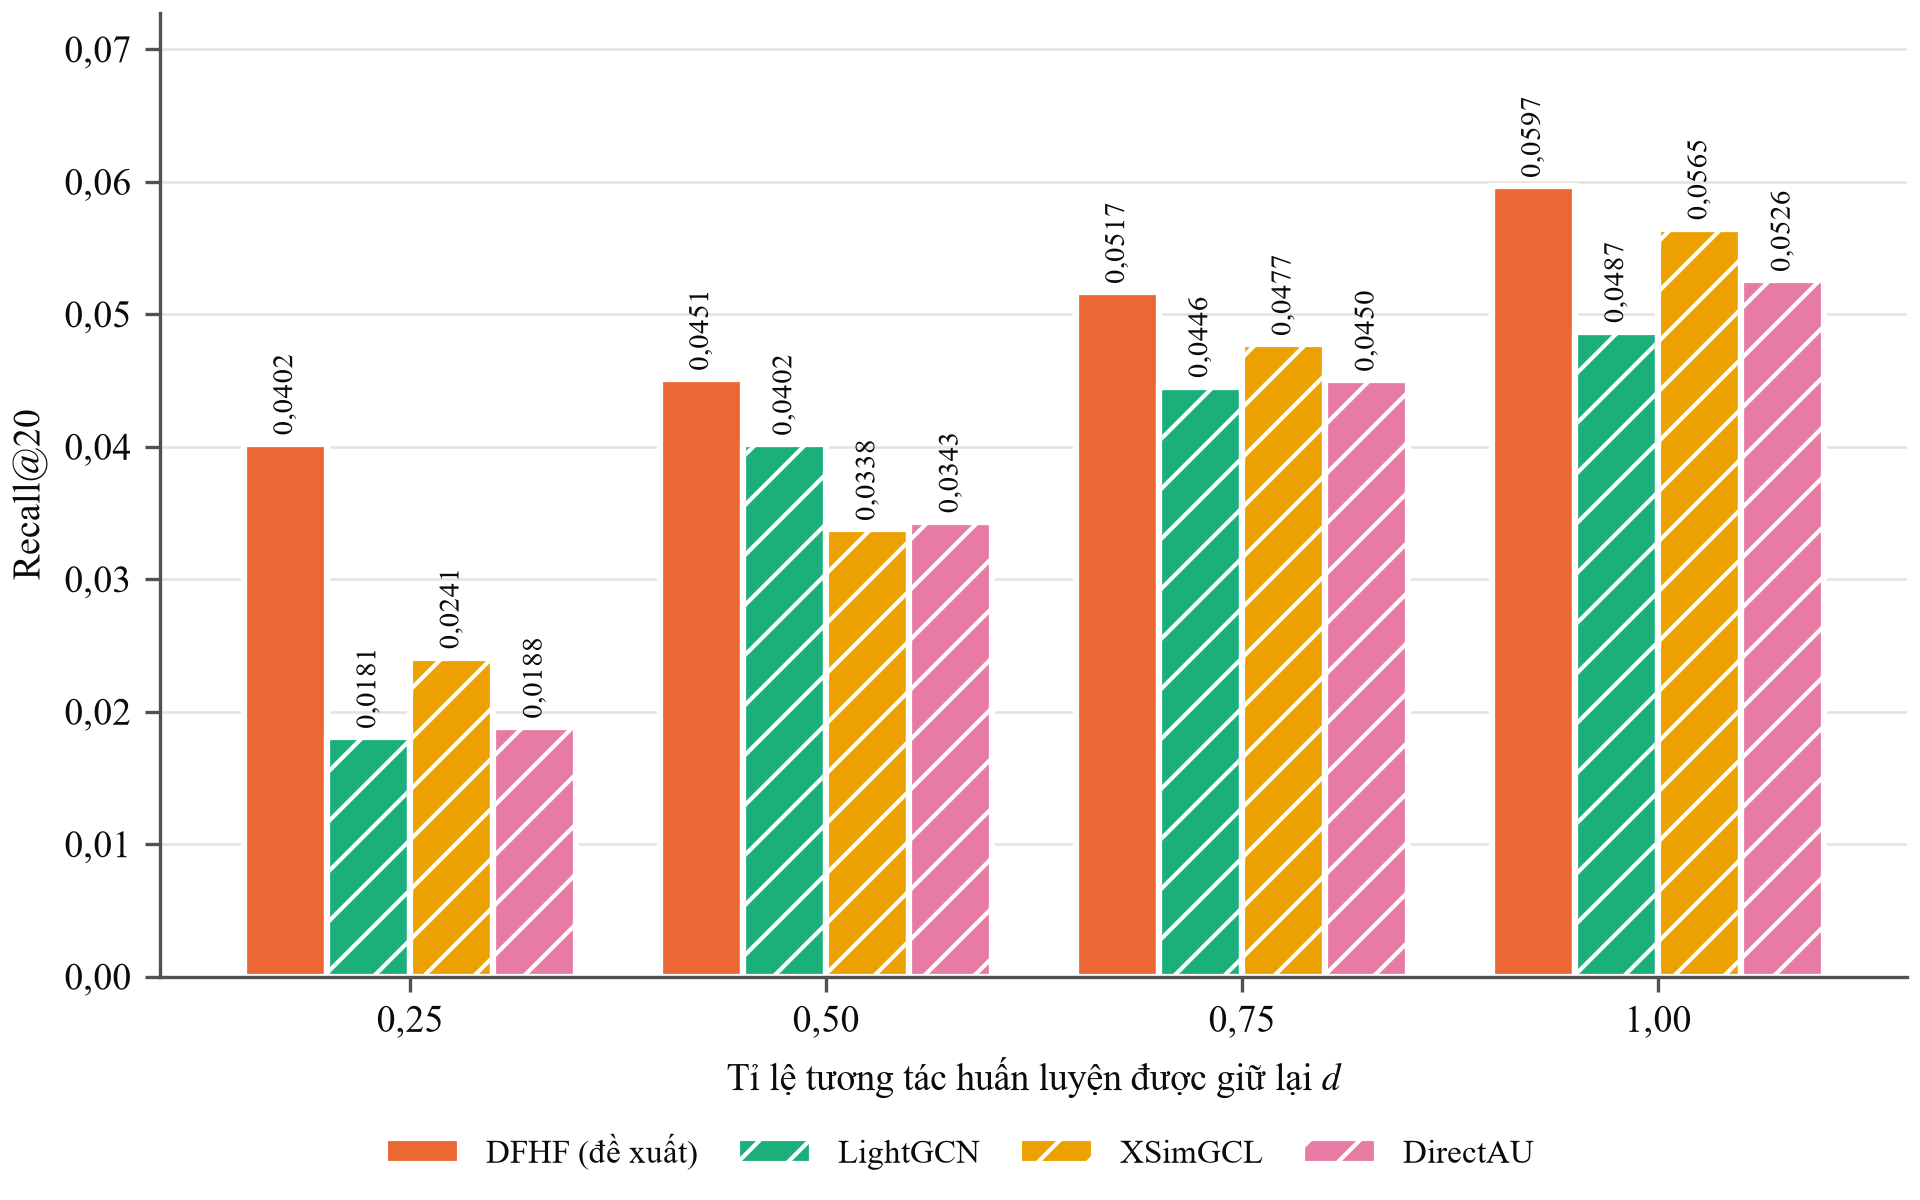
\includegraphics[width=0.75\linewidth]{H1_trained_density_recall20.png}
\caption{Recall@20 theo mức $d$, nhóm cần huấn luyện}
\label{fig:trained-recall20}
\end{figure}

Đường NDCG@K ở \figref{fig:trained-at-k} cho biết ưu thế của DFHF nằm ở đâu trong danh sách. Khi có đủ dữ liệu, DFHF đã hơn XSimGCL ngay tại $K=1$, với 0,00895 so với 0,00830, và khoảng cách tiếp tục tăng lên 0,00124 ở $K=10$ và 0,00163 ở $K=20$. Ưu thế của DFHF vì vậy có mặt từ gợi ý đầu tiên và tích lũy dần dọc theo danh sách. Ở $d=0{,}5$, DFHF cũng dẫn ngay từ $K=1$. Ở mức thưa nhất, đường của DFHF tách hẳn khỏi ba baseline từ đầu, với NDCG@1 bằng 0,00487 so với 0,00294 của DirectAU. Đây là phân tích mô tả, tính từ cùng danh sách dự đoán, không chọn lại checkpoint cho từng $K$.

\begin{figure}[H]
\centering
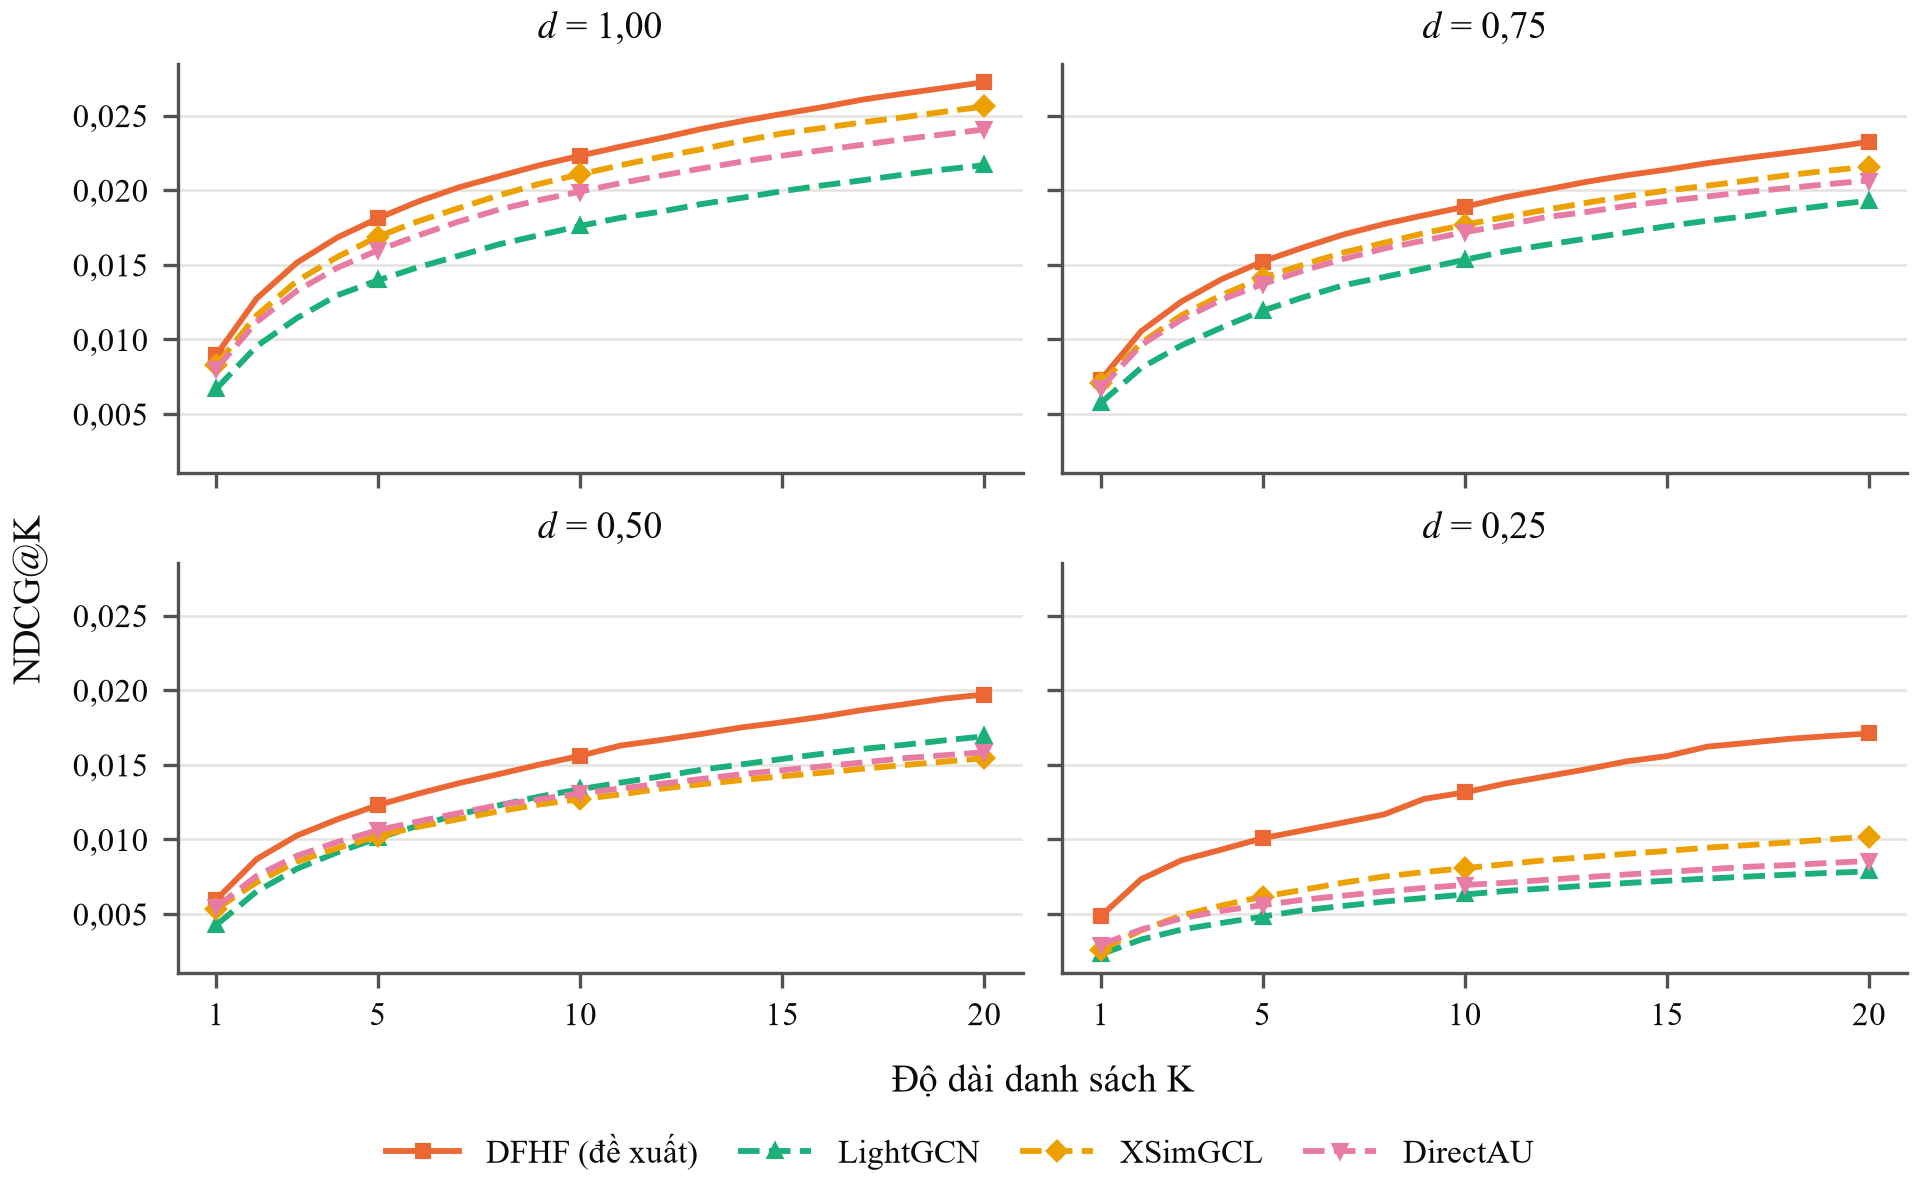
\includegraphics[width=0.75\linewidth]{H8_trained_ndcg_at_k.png}
\caption{NDCG@K, nhóm cần huấn luyện}
\label{fig:trained-at-k}
\end{figure}

\FloatBarrier
\subsubsection{Chất lượng khi dữ liệu thưa dần}

Những hình trên dễ dẫn tới kết luận rằng DFHF bền hơn hẳn khi dữ liệu thưa: DFHF cao nhất ở mọi mức, và khoảng cách với baseline tốt nhất lớn nhất ở mức thưa nhất. \Figref{fig:trained-density} đặt NDCG@20 của cả nhóm cạnh mốc MostPop, và chính mốc này cho thấy cách hiểu ``bền hơn'' là chưa đúng.

\begin{figure}[H]
\centering
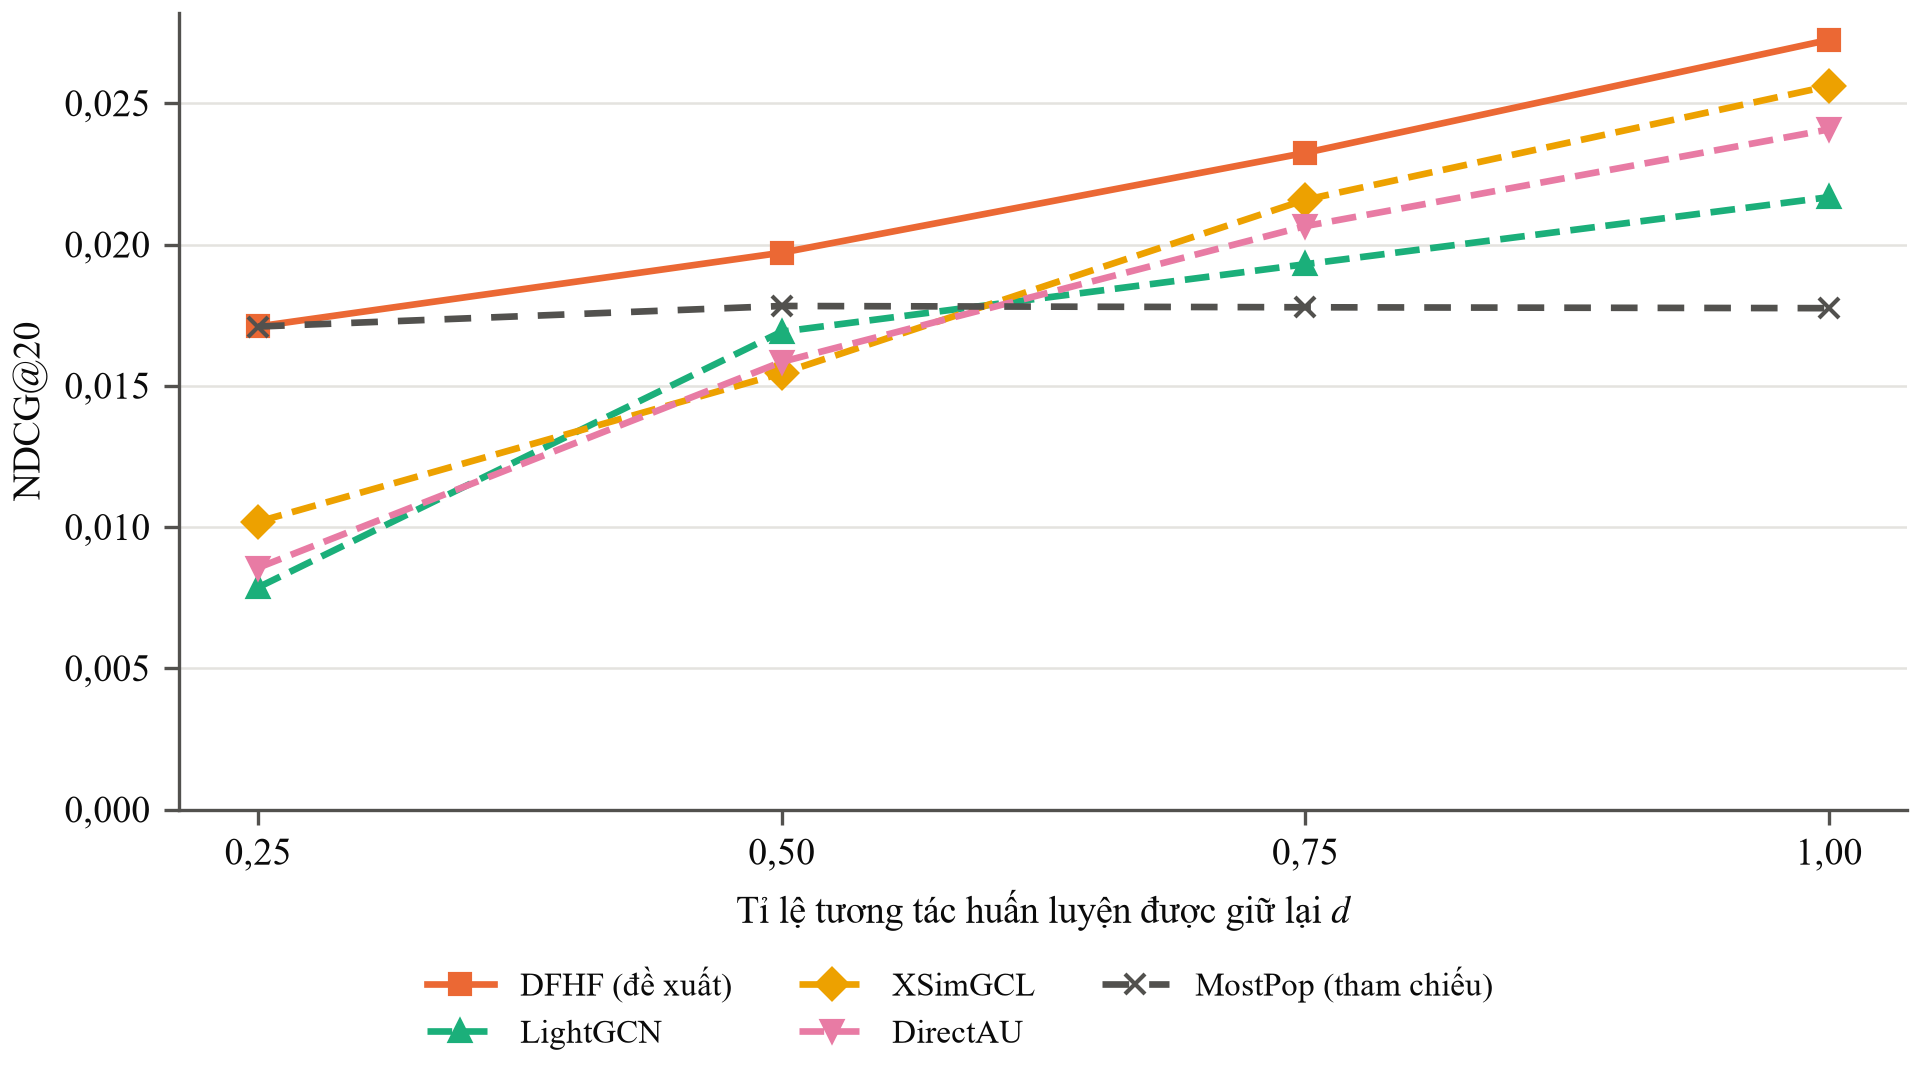
\includegraphics[width=0.75\linewidth]{H9_mostpop_trained_ndcg20.png}
\caption{NDCG@20 so với MostPop, nhóm cần huấn luyện}
\label{fig:trained-density}
\end{figure}

\Tabref{tab:trained-gain} làm rõ điều đó. Mức vượt MostPop của DFHF giảm đều từ 54\% xuống 31\%, 11\%, rồi chỉ còn 0,02\%: ở mức thưa nhất, DFHF chỉ còn ngang mốc độ phổ biến. Ba baseline thì đã xuống dưới MostPop từ $d=0{,}5$, và ở mức thưa nhất thấp hơn 40--54\%. Khoảng cách lớn giữa DFHF và XSimGCL ở mức thưa nhất vì thế không phản ánh khả năng cá nhân hóa tốt hơn. Nó phản ánh việc DFHF dừng lại ở mốc độ phổ biến trong khi các baseline tụt xuống dưới, và gợi ý cần xem xét vai trò của hệ số chặn khi lịch sử quá ngắn.

\begin{table}[H]
\centering
\small
\begin{tabular}{@{}lrrrr@{}}
\toprule
& $d=1$ & $d=0{,}75$ & $d=0{,}5$ & $d=0{,}25$ \\
\midrule
MostPop (NDCG@20) & 0{,}01775 & 0{,}01778 & 0{,}01782 & 0{,}01710 \\
\midrule
DFHF & $+53{,}5\%$ & $+30{,}7\%$ & $+10{,}6\%$ & $+0{,}02\%$ \\
LightGCN & $+22{,}1\%$ & $+8{,}6\%$ & $-5{,}1\%$ & $-54{,}0\%$ \\
XSimGCL & $+44{,}3\%$ & $+21{,}4\%$ & $-13{,}4\%$ & $-40{,}4\%$ \\
DirectAU & $+35{,}7\%$ & $+16{,}2\%$ & $-11{,}1\%$ & $-50{,}0\%$ \\
\bottomrule
\end{tabular}
\caption{Mức vượt MostPop, nhóm cần huấn luyện}
\label{tab:trained-gain}
\end{table}

Tỉ lệ duy trì đi tới cùng kết luận từ một góc khác. Theo NDCG@10 ở \figref{fig:trained-retention-ndcg10}, khi dữ liệu còn khá dày, DFHF không suy giảm chậm hơn các baseline: ở cả $d=0{,}75$ và $d=0{,}5$, nó đều giữ ít hơn LightGCN. Chỉ ở mức thưa nhất, DFHF mới tách hẳn lên, giữ 58,9\% so với 35--38\% của ba baseline. Sự bền vững của DFHF vì thế chỉ xuất hiện ở đúng mức mà điểm số của nó chạm mốc MostPop.

\begin{figure}[H]
\centering
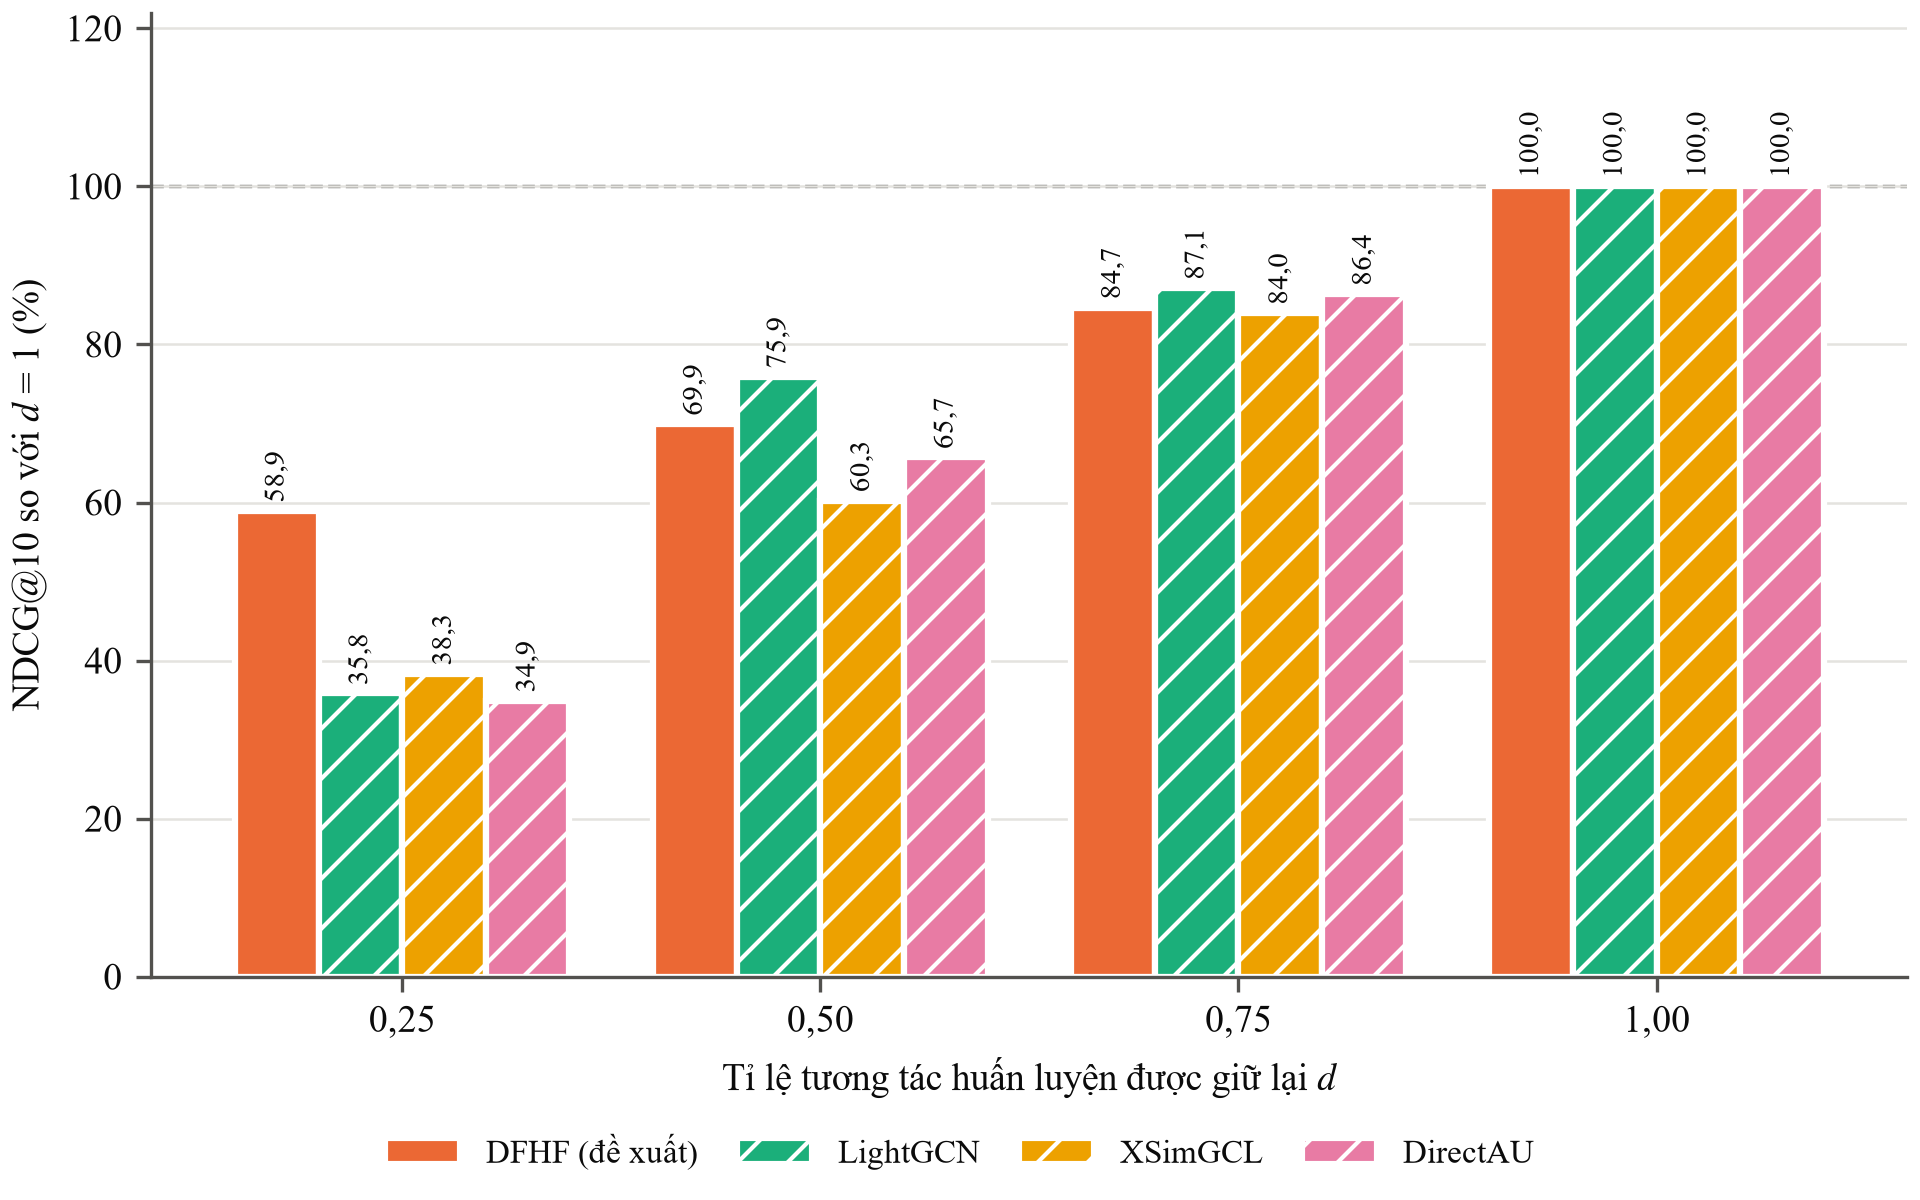
\includegraphics[width=0.75\linewidth]{H4_trained_retention_ndcg10.png}
\caption{Tỉ lệ duy trì NDCG@10, nhóm cần huấn luyện}
\label{fig:trained-retention-ndcg10}
\end{figure}

NDCG@20 ở \figref{fig:trained-retention-ndcg20} cho cùng mẫu hình: ở mức thưa nhất, DFHF giữ 62,8\% so với 36--40\% của các baseline, nhưng ở $d=0{,}5$, LightGCN giữ nhiều nhất, 78,0\% so với 72,3\% của DFHF, một phần vì LightGCN xuất phát từ mức thấp hơn. Khi các mô hình có điểm khởi đầu và mức sàn khác nhau như vậy, tỉ lệ duy trì không cho biết mô hình nào học tốt hơn.

\begin{figure}[H]
\centering
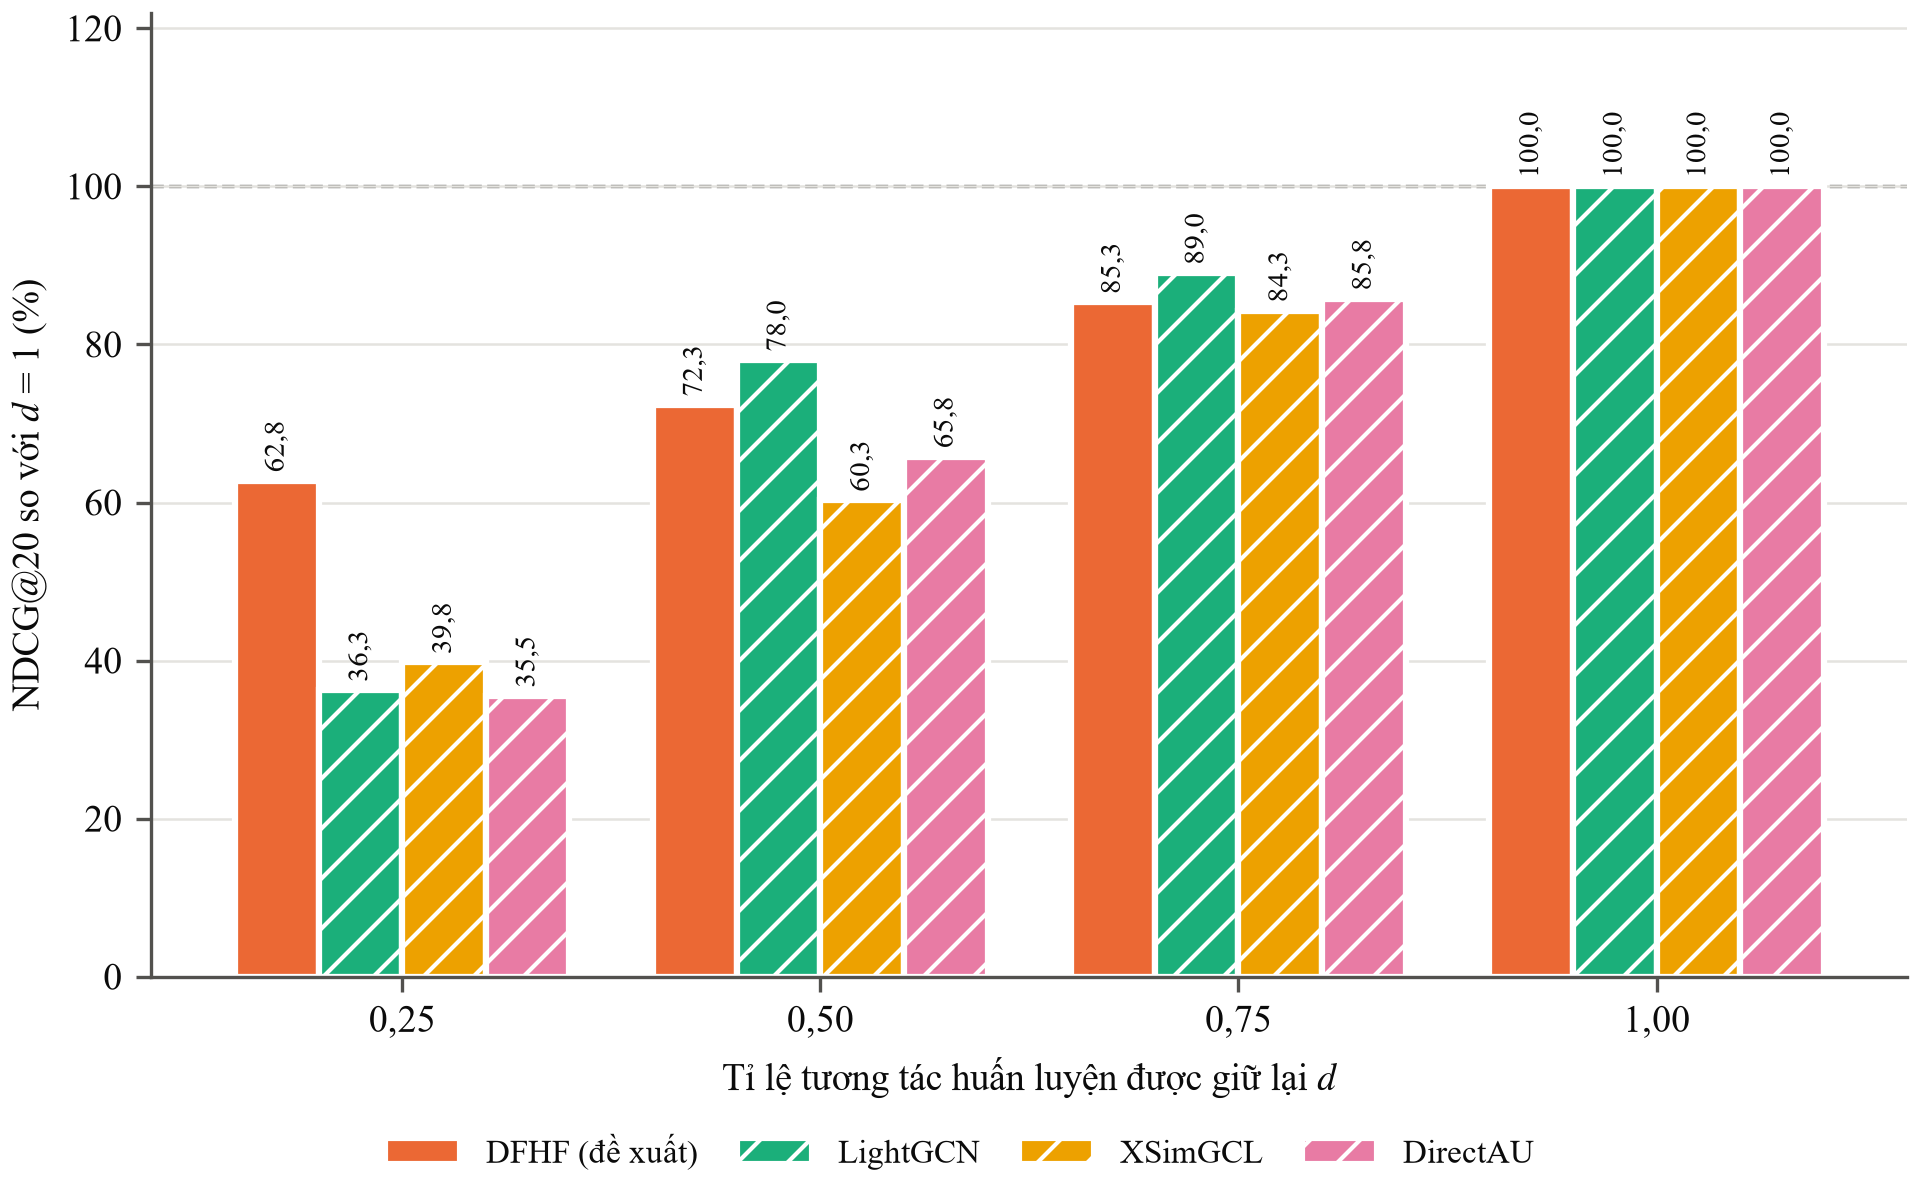
\includegraphics[width=0.75\linewidth]{H4_trained_retention_ndcg20.png}
\caption{Tỉ lệ duy trì NDCG@20, nhóm cần huấn luyện}
\label{fig:trained-retention-ndcg20}
\end{figure}

Recall@10 ở \figref{fig:trained-retention-recall10} lặp lại điều này: LightGCN giữ nhiều nhất ở $d=0{,}5$, còn DFHF chỉ vượt lên ở mức thưa nhất. Giữ được một phần chất lượng chưa cho biết phần đó đến từ lịch sử hay từ hệ số chặn; muốn biết, cần đối chiếu với MostPop và với nhóm người dùng chỉ còn một tương tác ở mục dưới.

\begin{figure}[H]
\centering
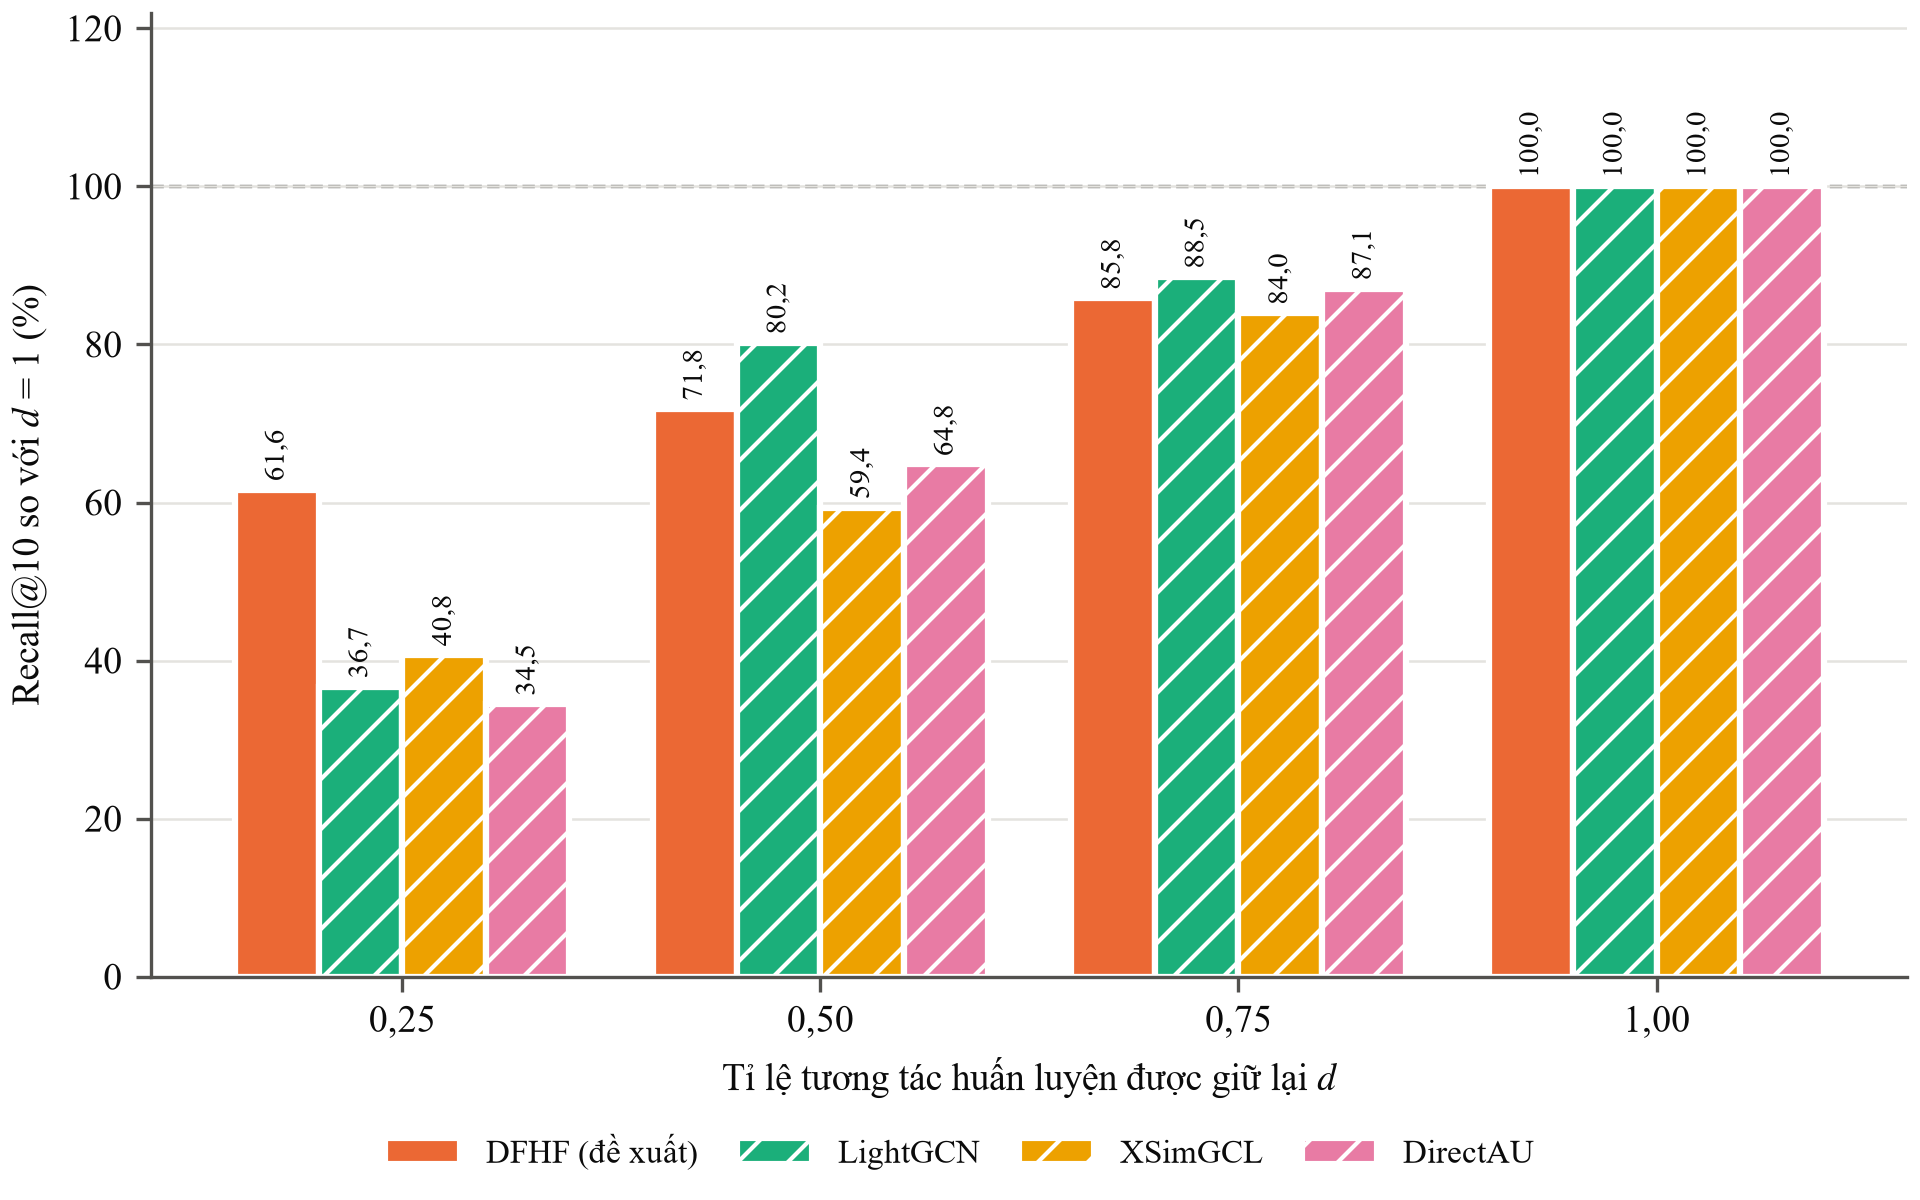
\includegraphics[width=0.75\linewidth]{H4_trained_retention_recall10.png}
\caption{Tỉ lệ duy trì Recall@10, nhóm cần huấn luyện}
\label{fig:trained-retention-recall10}
\end{figure}

Với DFHF, Recall@20 ở \figref{fig:trained-retention-recall20} cho tỉ lệ duy trì cao nhất trong bốn thước đo, 67,4\% ở mức thưa nhất, trong khi LightGCN vẫn giữ nhiều nhất ở $d=0{,}75$ và $d=0{,}5$. Recall@20 của DFHF giữ được nhiều hơn NDCG@20, 67,4\% so với 62,8\%, nghĩa là mô hình vẫn đưa được mục tiêu vào danh sách nhưng ở vị trí thấp hơn trước.

\begin{figure}[H]
\centering
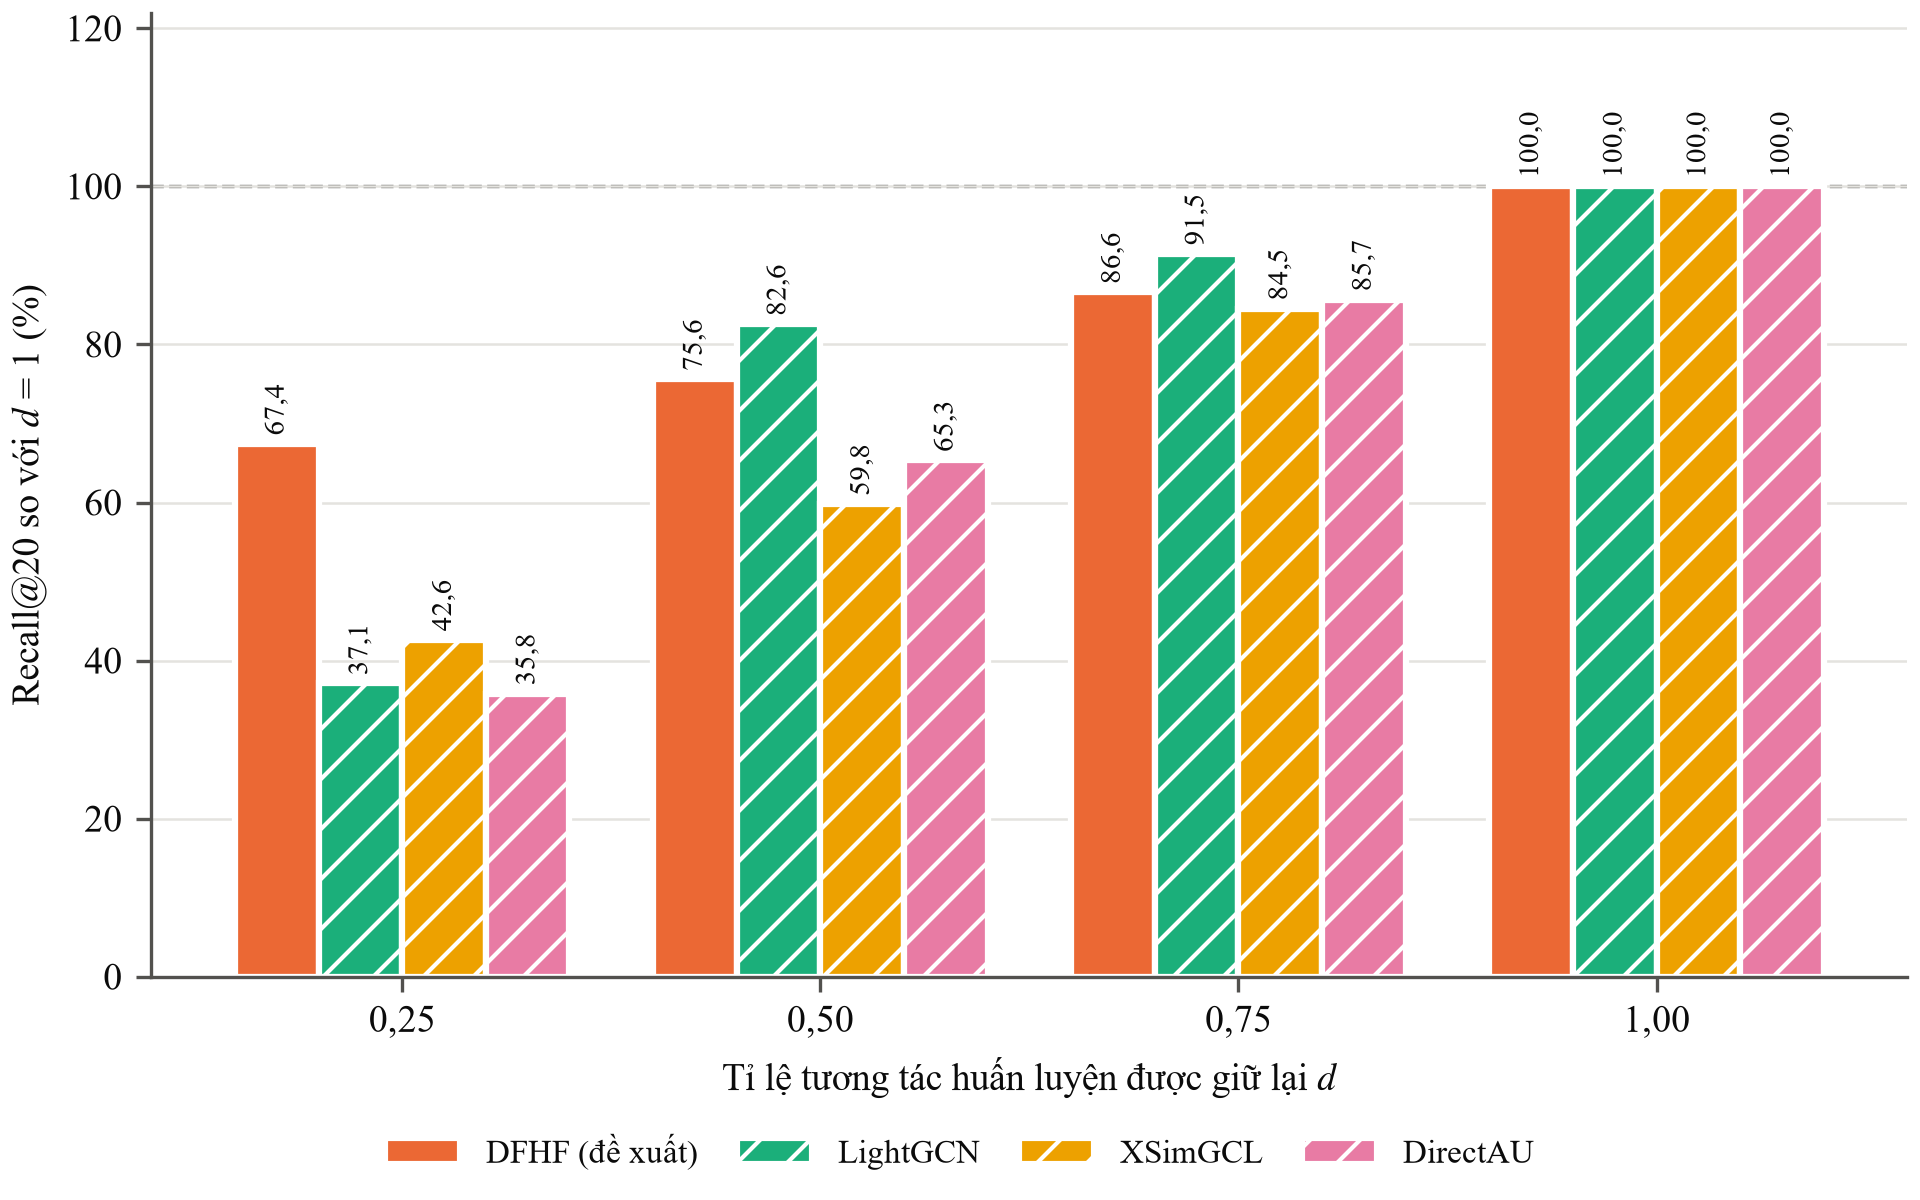
\includegraphics[width=0.75\linewidth]{H4_trained_retention_recall20.png}
\caption{Tỉ lệ duy trì Recall@20, nhóm cần huấn luyện}
\label{fig:trained-retention-recall20}
\end{figure}

\FloatBarrier
\subsubsection{Nguồn tín hiệu khi dữ liệu thưa}

Mức sàn gần MostPop của DFHF có một cơ chế cụ thể, đã mô tả ở Mục~\ref{sec:dfhf-representation}. Người dùng chỉ còn một tương tác nhận vector lịch sử bằng 0, nên được xếp hạng chỉ bằng hệ số chặn $b$, tức một thứ tự chung do vector chặn đã học quyết định, không nhất thiết trùng MostPop. Ở mức thưa nhất, nhóm người dùng này chiếm 68\%. \Tabref{tab:degree-split} xác nhận trực tiếp: trên người dùng bậc 1, DFHF đạt 0,01757, gần như trùng với 0,01746 của MostPop. Các baseline thì phải học một vector người dùng từ đúng một tương tác; vector đó nhiễu và cho xếp hạng kém cả độ phổ biến.

\begin{table}[H]
\centering
\small
\begin{tabular}{@{}lrrr@{}}
\toprule
Mô hình & Bậc 1 ($n=72.889$) & Bậc $\ge2$ ($n=34.198$) & Tất cả \\
\midrule
DFHF & 0,01757 & 0,01609 & 0,01710 \\
LightGCN & 0,00788 & 0,00782 & 0,00786 \\
XSimGCL & 0,01041 & 0,00970 & 0,01019 \\
DirectAU & 0,00849 & 0,00870 & 0,00856 \\
\midrule
MostPop (tham chiếu) & 0,01746 & 0,01631 & 0,01710 \\
\bottomrule
\end{tabular}
\caption{NDCG@20 theo số tương tác còn lại ($d=0{,}25$)}
\label{tab:degree-split}
\end{table}

Với người dùng còn từ hai tương tác trở lên, DFHF đạt 0,01609, vẫn thấp hơn một chút so với 0,01631 của MostPop. Ở mức thưa này, vì vậy, chưa có bằng chứng rằng DFHF khai thác lịch sử tốt hơn một cách xếp hạng không cá nhân hóa. Kết quả gợi ý rằng khi dữ liệu rất thưa, một phương án dự phòng tốt có thể quan trọng hơn khả năng biểu diễn của mô hình; nhận định này chưa được kiểm tra bằng cách cho các baseline dùng cùng phương án dự phòng.

Nếu phần lớn người dùng được xếp hạng chỉ bằng hệ số chặn, danh sách gợi ý của DFHF phải tập trung hơn vào sản phẩm phổ biến khi dữ liệu thưa, và \tabref{tab:trained-popularity} cho thấy đúng như vậy. Từ $d=1$ xuống mức thưa nhất, độ phổ biến trung bình sau biến đổi log của các sản phẩm DFHF gợi ý tăng từ 5,84 lên 7,10, rất gần mức 7,16 của chính MostPop, còn độ phủ danh mục giảm từ 32,1\% xuống 12,9\%. Xu hướng tập trung này không riêng DFHF: độ phổ biến của XSimGCL cũng tăng, và độ phủ của LightGCN giảm từ 47,0\% xuống 7,5\%. Điểm riêng của DFHF là mức tập trung cao nhất nhóm đi cùng NDCG@20 bằng MostPop thay vì thấp hơn. Bảng chưa tách được ảnh hưởng của hệ số chặn, biểu diễn lịch sử và tập ứng viên, và mức phổ biến gần bằng MostPop cũng chưa cho biết hai danh sách trùng nhau đến đâu.

DirectAU đi theo chiều ngược lại: độ phủ tăng từ 11,9\% lên 38,7\% dù NDCG@20 giảm. Cùng với diễn biến độ phổ biến, kết quả này cho thấy phạm vi sản phẩm được gợi ý và khả năng đưa đúng mục tiêu lên đầu là hai khía cạnh khác nhau; không thể dùng riêng độ phủ để xếp hạng chất lượng các mô hình.

\begin{table}[H]
\centering
\small
\begin{tabular}{@{}lrrrr@{}}
\toprule
& $d=1$ & $d=0{,}75$ & $d=0{,}5$ & $d=0{,}25$ \\
\midrule
\multicolumn{5}{@{}l}{Độ phổ biến trung bình (log)} \\
DFHF & 5{,}84 & 6{,}09 & 6{,}67 & 7{,}10 \\
LightGCN & 5{,}91 & 6{,}18 & 6{,}46 & 6{,}06 \\
XSimGCL & 5{,}82 & 5{,}89 & 6{,}02 & 6{,}46 \\
DirectAU & 5{,}64 & 5{,}66 & 5{,}75 & 5{,}47 \\
MostPop (tham chiếu) & 7{,}17 & 7{,}17 & 7{,}17 & 7{,}16 \\
\midrule
\multicolumn{5}{@{}l}{Độ phủ danh mục trong top-20 (\%)} \\
DFHF & 32{,}1 & 30{,}8 & 21{,}1 & 12{,}9 \\
LightGCN & 47{,}0 & 33{,}7 & 26{,}8 & 7{,}5 \\
XSimGCL & 6{,}8 & 6{,}7 & 5{,}9 & 2{,}6 \\
DirectAU & 11{,}9 & 13{,}8 & 18{,}3 & 38{,}7 \\
\bottomrule
\end{tabular}
\caption{Độ phổ biến và độ phủ, nhóm cần huấn luyện}
\label{tab:trained-popularity}
\end{table}

\FloatBarrier
\subsubsection{Chất lượng theo độ dài lịch sử người dùng}

Chia người dùng theo độ dài lịch sử như ở \figref{fig:trained-groups}, hiện tượng người dùng nhiều tương tác được gợi ý kém hơn lại xuất hiện. Khi có đủ dữ liệu, NDCG@20 của DFHF giảm từ 0,0296 ở nhóm ngắn nhất xuống 0,0198 ở nhóm dài nhất, và cả ba baseline cũng vậy. Điểm riêng ở đây là với người dùng có từ 10 tương tác trở lên, XSimGCL nhỉnh hơn DFHF, 0,0202 so với 0,0198. Một giả thuyết là DFHF gộp cả lịch sử thành một vector duy nhất bằng phép cộng chuẩn hóa; với lịch sử dài và đa dạng, phép gộp này làm mờ các sở thích khác nhau, trong khi một vector người dùng học riêng có thể giữ chúng tốt hơn.

Khi dữ liệu thưa đi, DFHF lại dẫn ở cả ba nhóm tại mọi mức $d\le0{,}75$. Ở mức thưa nhất, NDCG@20 của DFHF ở ba nhóm chỉ còn dao động từ 0,0153 đến 0,0181, hẹp hơn nhiều so với ở $d=1$: khi phần lớn người dùng được xếp hạng chủ yếu bằng hệ số chặn, độ dài lịch sử gốc không còn tạo ra nhiều khác biệt. Các giá trị theo nhóm chỉ mang tính mô tả.

\begin{figure}[H]
\centering
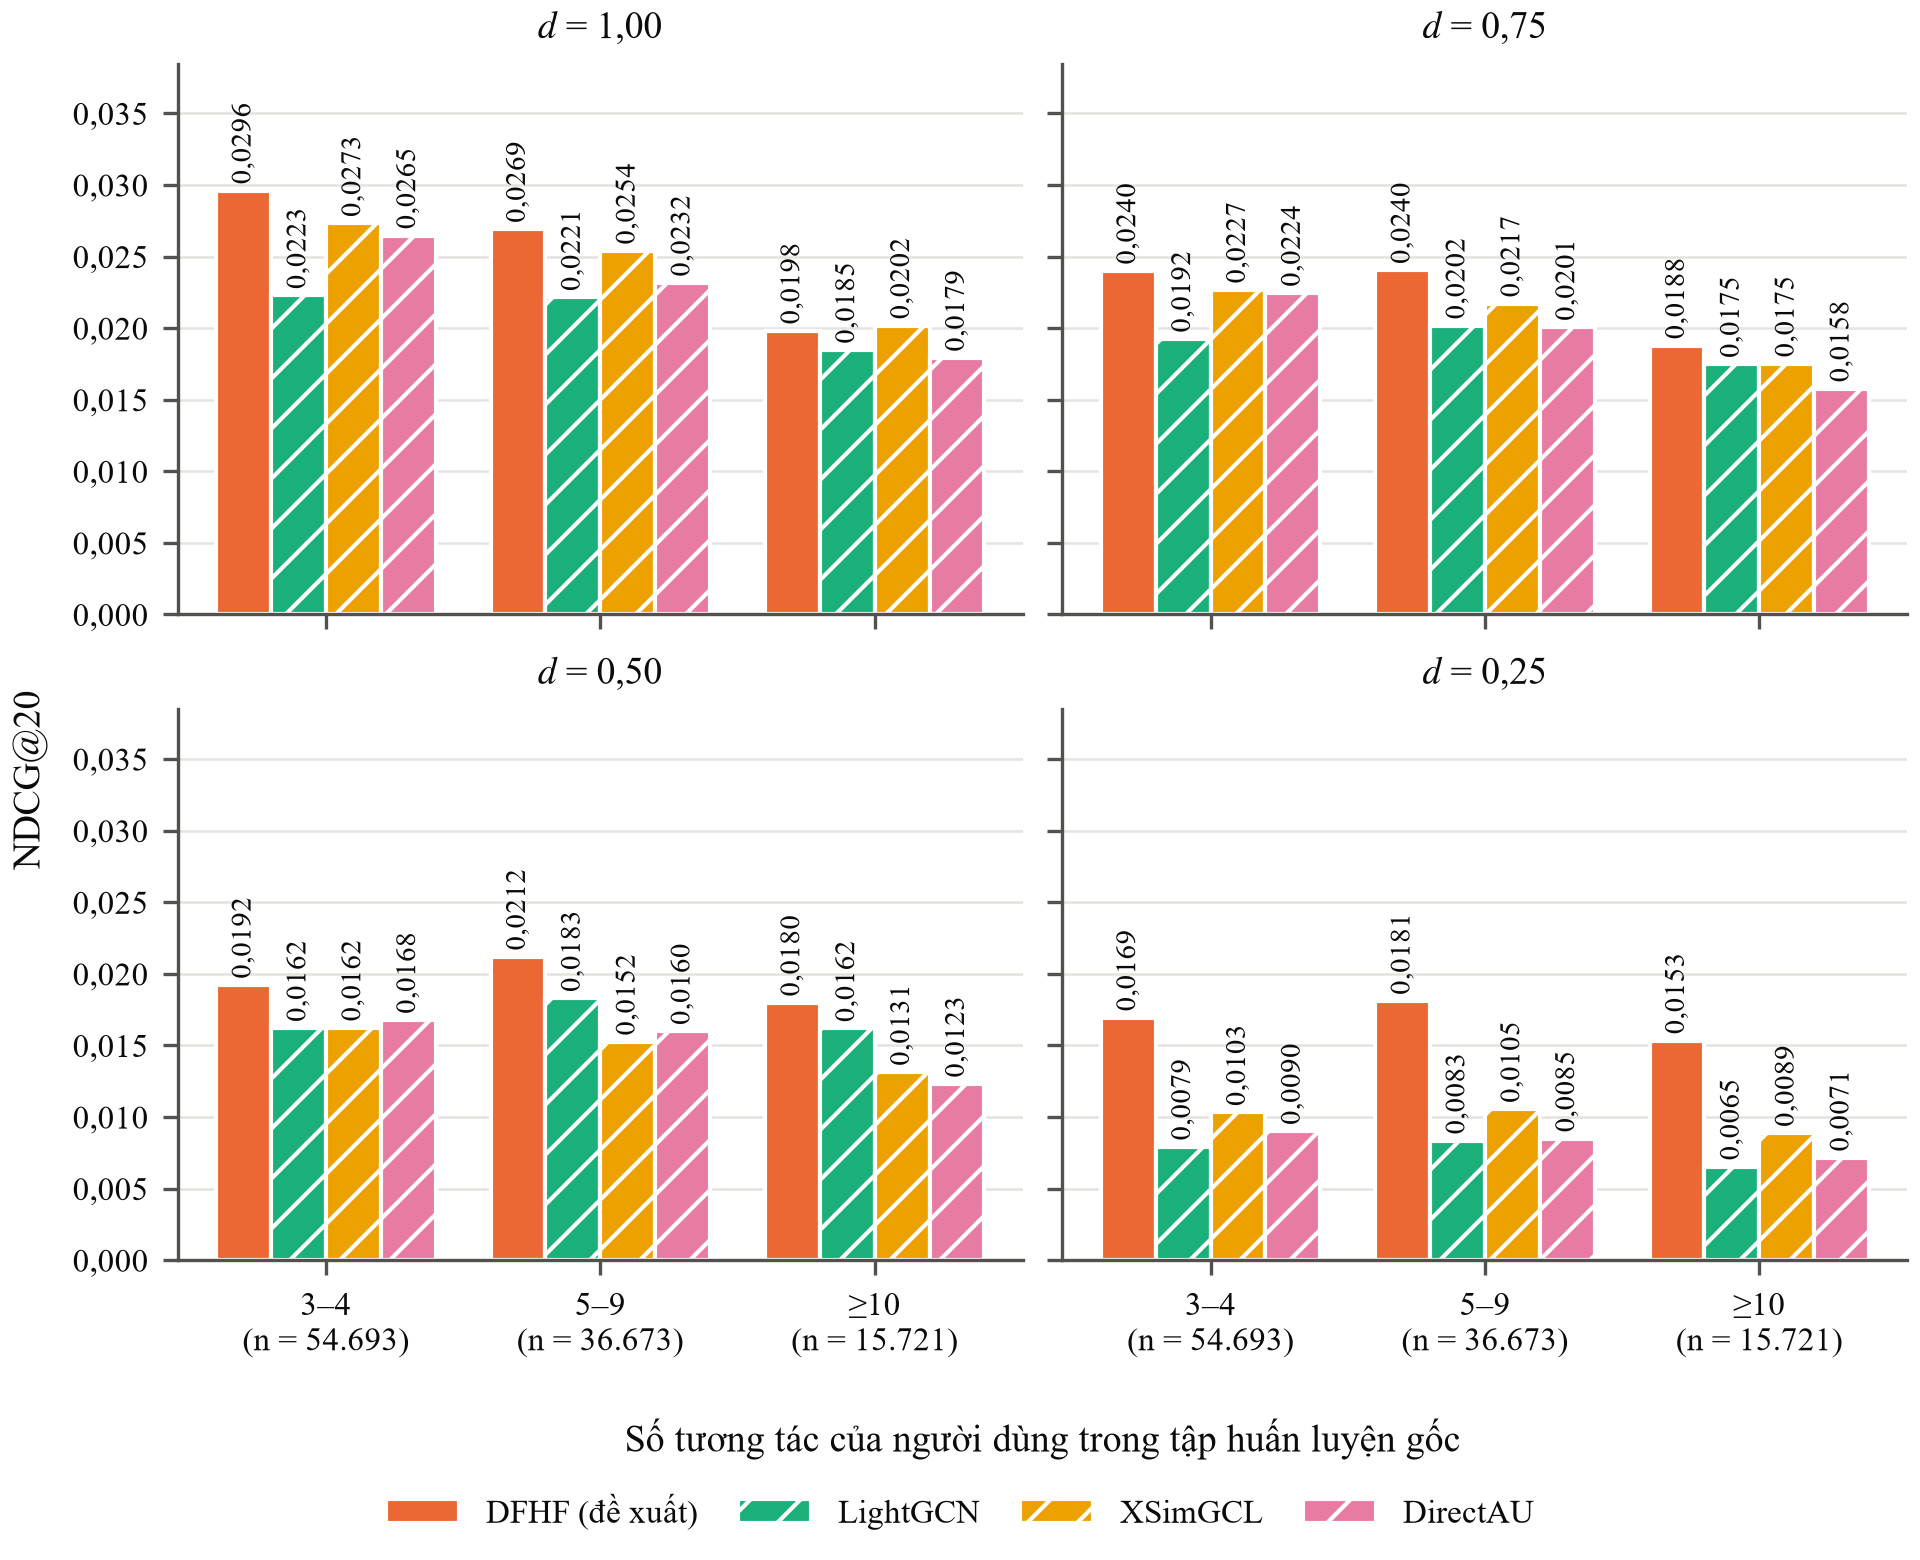
\includegraphics[width=0.68\linewidth]{H5_trained_user_groups_ndcg20.png}
\caption{NDCG@20 theo độ dài lịch sử, nhóm cần huấn luyện}
\label{fig:trained-groups}
\end{figure}

Thu hẹp về mười vị trí đầu như ở \figref{fig:trained-groups-ndcg10}, mẫu hình vẫn vậy: ở $d=1$, XSimGCL cao hơn DFHF ở nhóm lịch sử dài nhất, 0,0164 so với 0,0156, còn ở mọi trường hợp khác DFHF dẫn cả ba nhóm. Khoảng cách lớn nhất ở mức thưa nhất, khi DFHF đạt 0,0120 đến 0,0136 ở ba nhóm, còn baseline tốt nhất chỉ đạt 0,0071 đến 0,0084. Điểm trung bình cao nhất vì thế không có nghĩa DFHF cao nhất ở mọi nhóm và mọi phần của danh sách.

\begin{figure}[H]
\centering
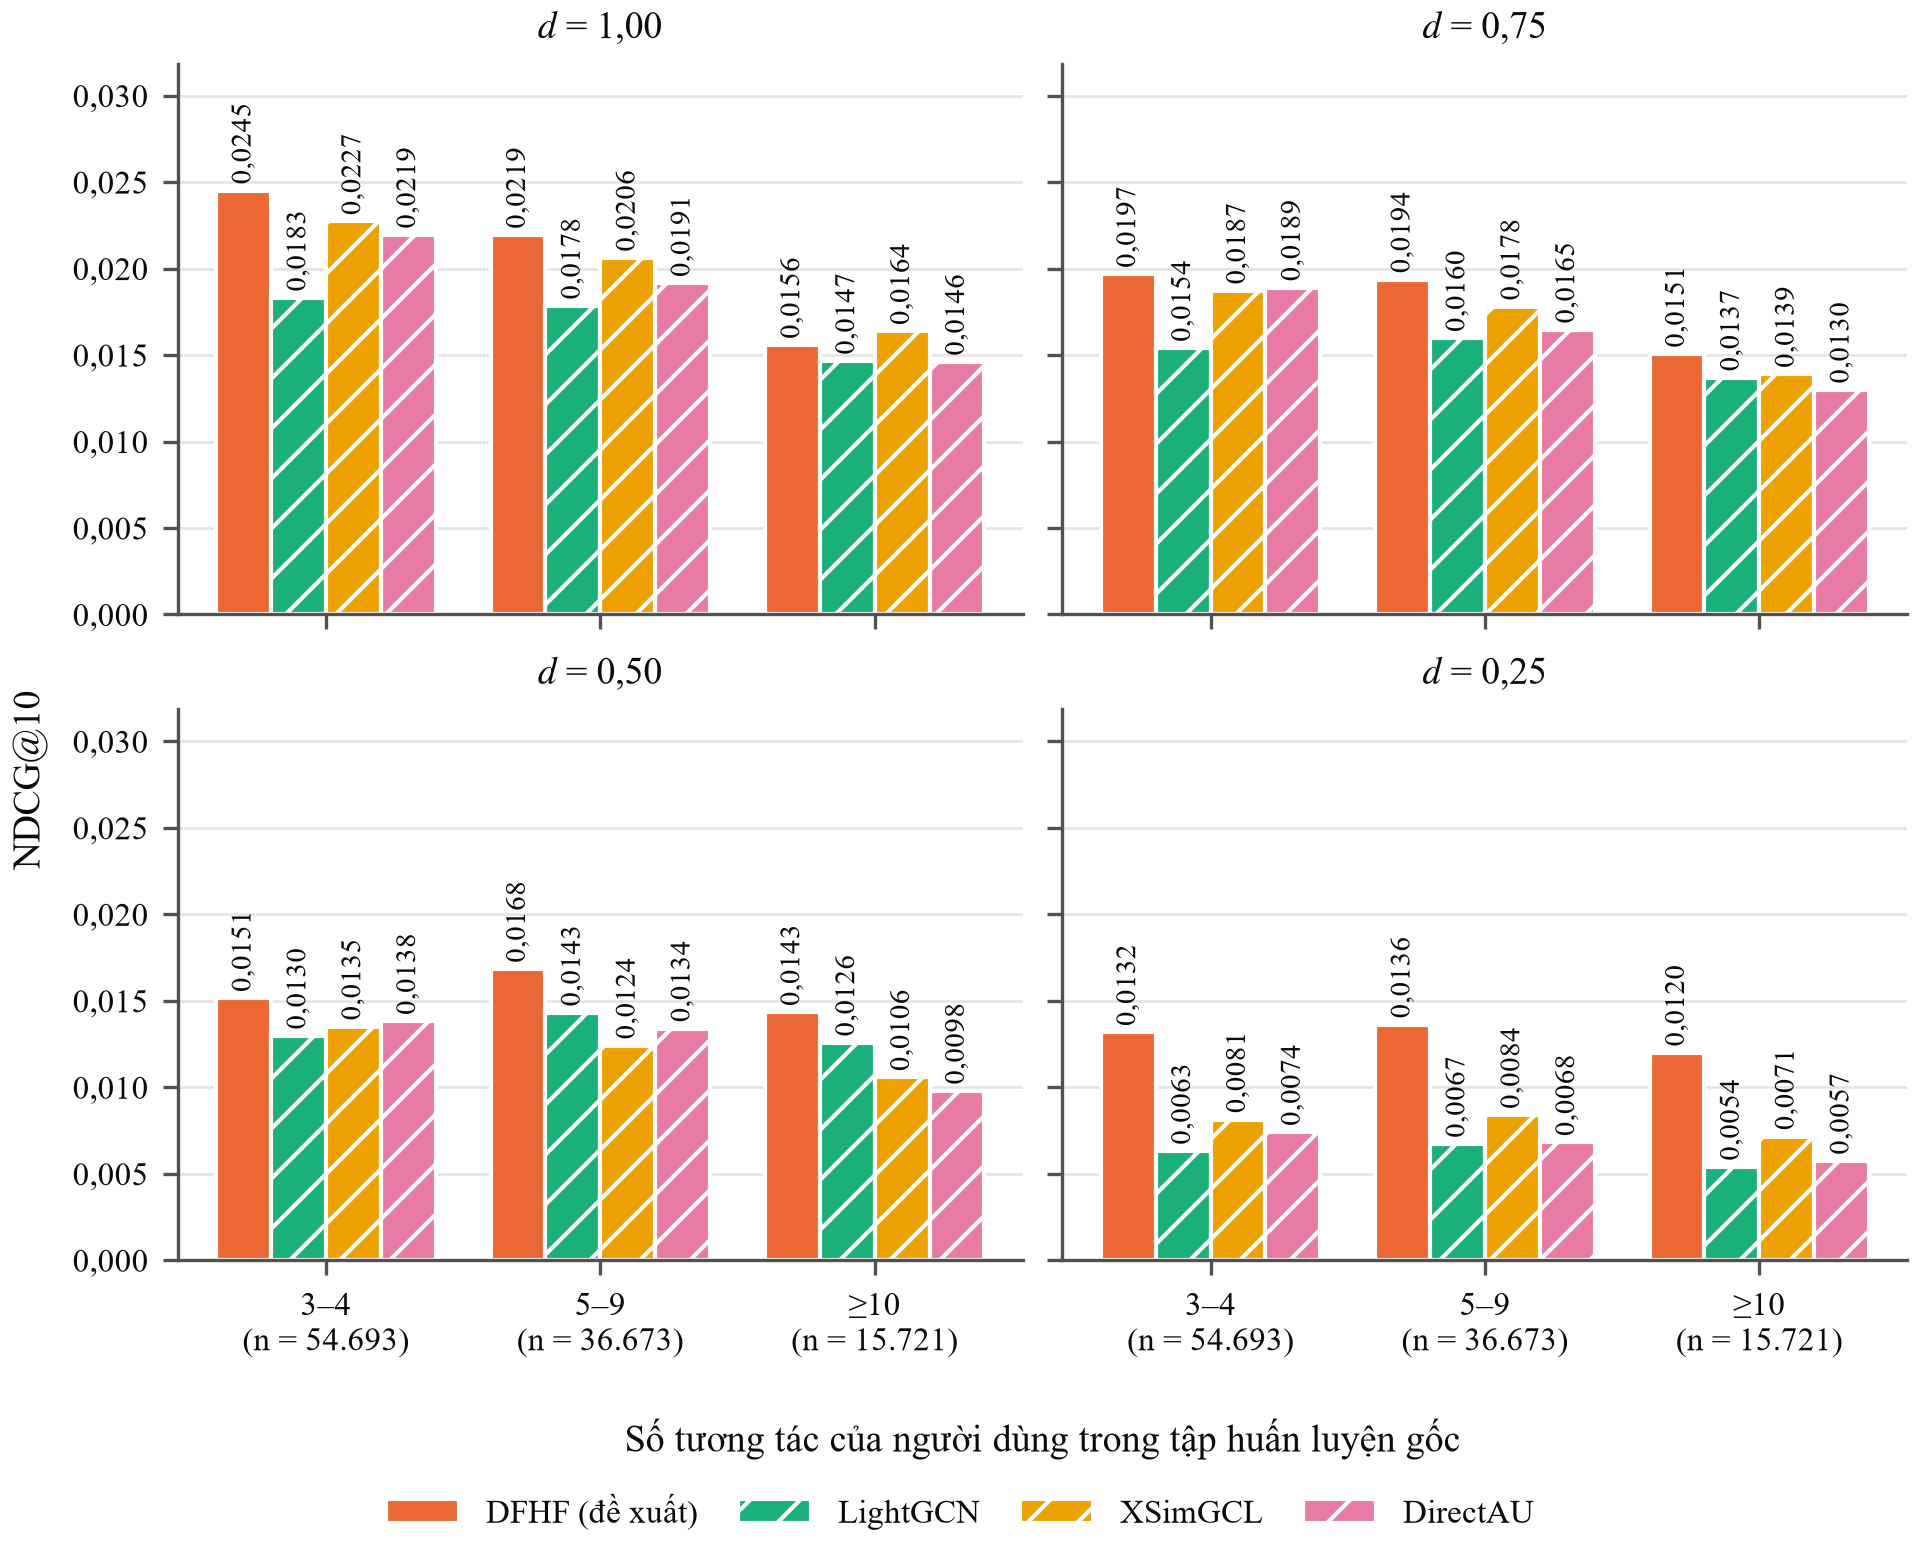
\includegraphics[width=0.68\linewidth]{H5_trained_user_groups_ndcg10.png}
\caption{NDCG@10 theo độ dài lịch sử, nhóm cần huấn luyện}
\label{fig:trained-groups-ndcg10}
\end{figure}

Recall@10 ở \figref{fig:trained-groups-recall10} cho biết ưu thế của DFHF đến từ đâu. Khi có đủ dữ liệu, DFHF dẫn ở hai nhóm lịch sử ngắn, chẳng hạn 0,0431 so với 0,0409 của XSimGCL ở nhóm 3--4, nhưng ở nhóm dài nhất XSimGCL lại cao hơn, 0,0303 so với 0,0289. Ưu thế trung bình của DFHF như vậy chủ yếu đến từ người dùng lịch sử ngắn, cũng là nhóm đông nhất; với người dùng lịch sử dài, DFHF không hơn XSimGCL khi dữ liệu đầy đủ.

\begin{figure}[H]
\centering
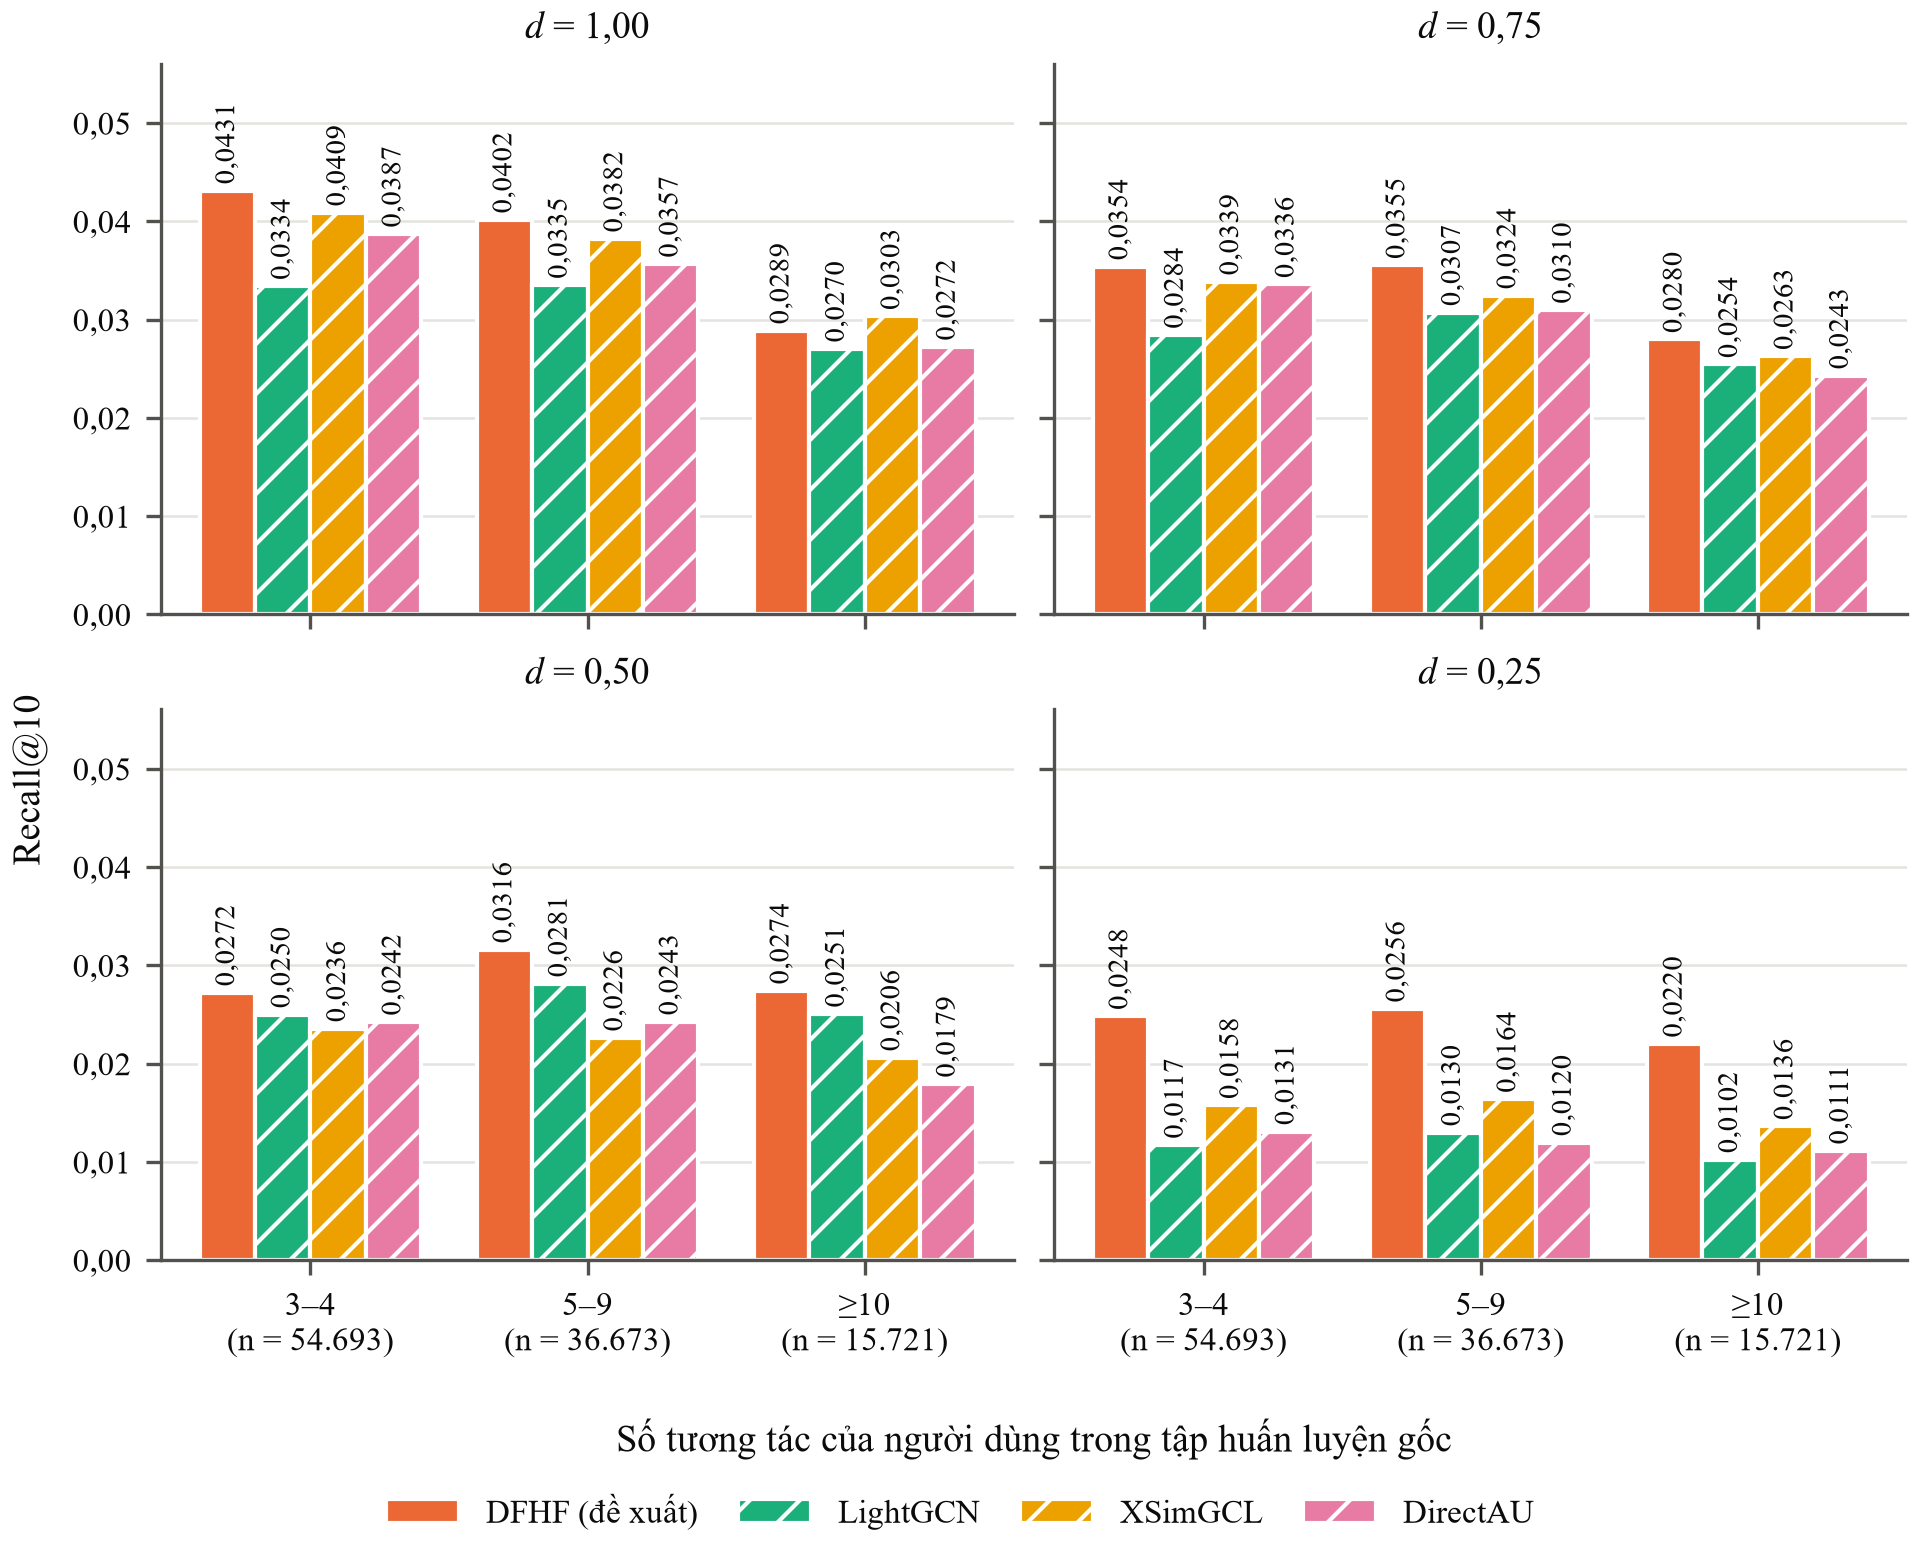
\includegraphics[width=0.68\linewidth]{H5_trained_user_groups_recall10.png}
\caption{Recall@10 theo độ dài lịch sử, nhóm cần huấn luyện}
\label{fig:trained-groups-recall10}
\end{figure}

Recall@20 ở \figref{fig:trained-groups-recall20} cũng giảm theo độ dài lịch sử khi có đủ dữ liệu, và ở nhóm dài nhất XSimGCL gần như bằng DFHF. Ở $d=0{,}5$, xu hướng này không còn đơn điệu: Recall@20 của DFHF ở nhóm 5--9 cao hơn nhóm 3--4, và LightGCN ở nhóm dài nhất cao hơn nhóm ngắn nhất, giống chiều đảo đã thấy ở nhóm giải trực tiếp. Các hình Recall chỉ đo khả năng tìm đúng mục tiêu, chưa đo mức hữu ích của những sản phẩm phù hợp khác không trùng với mục tiêu kiểm tra.

\begin{figure}[H]
\centering
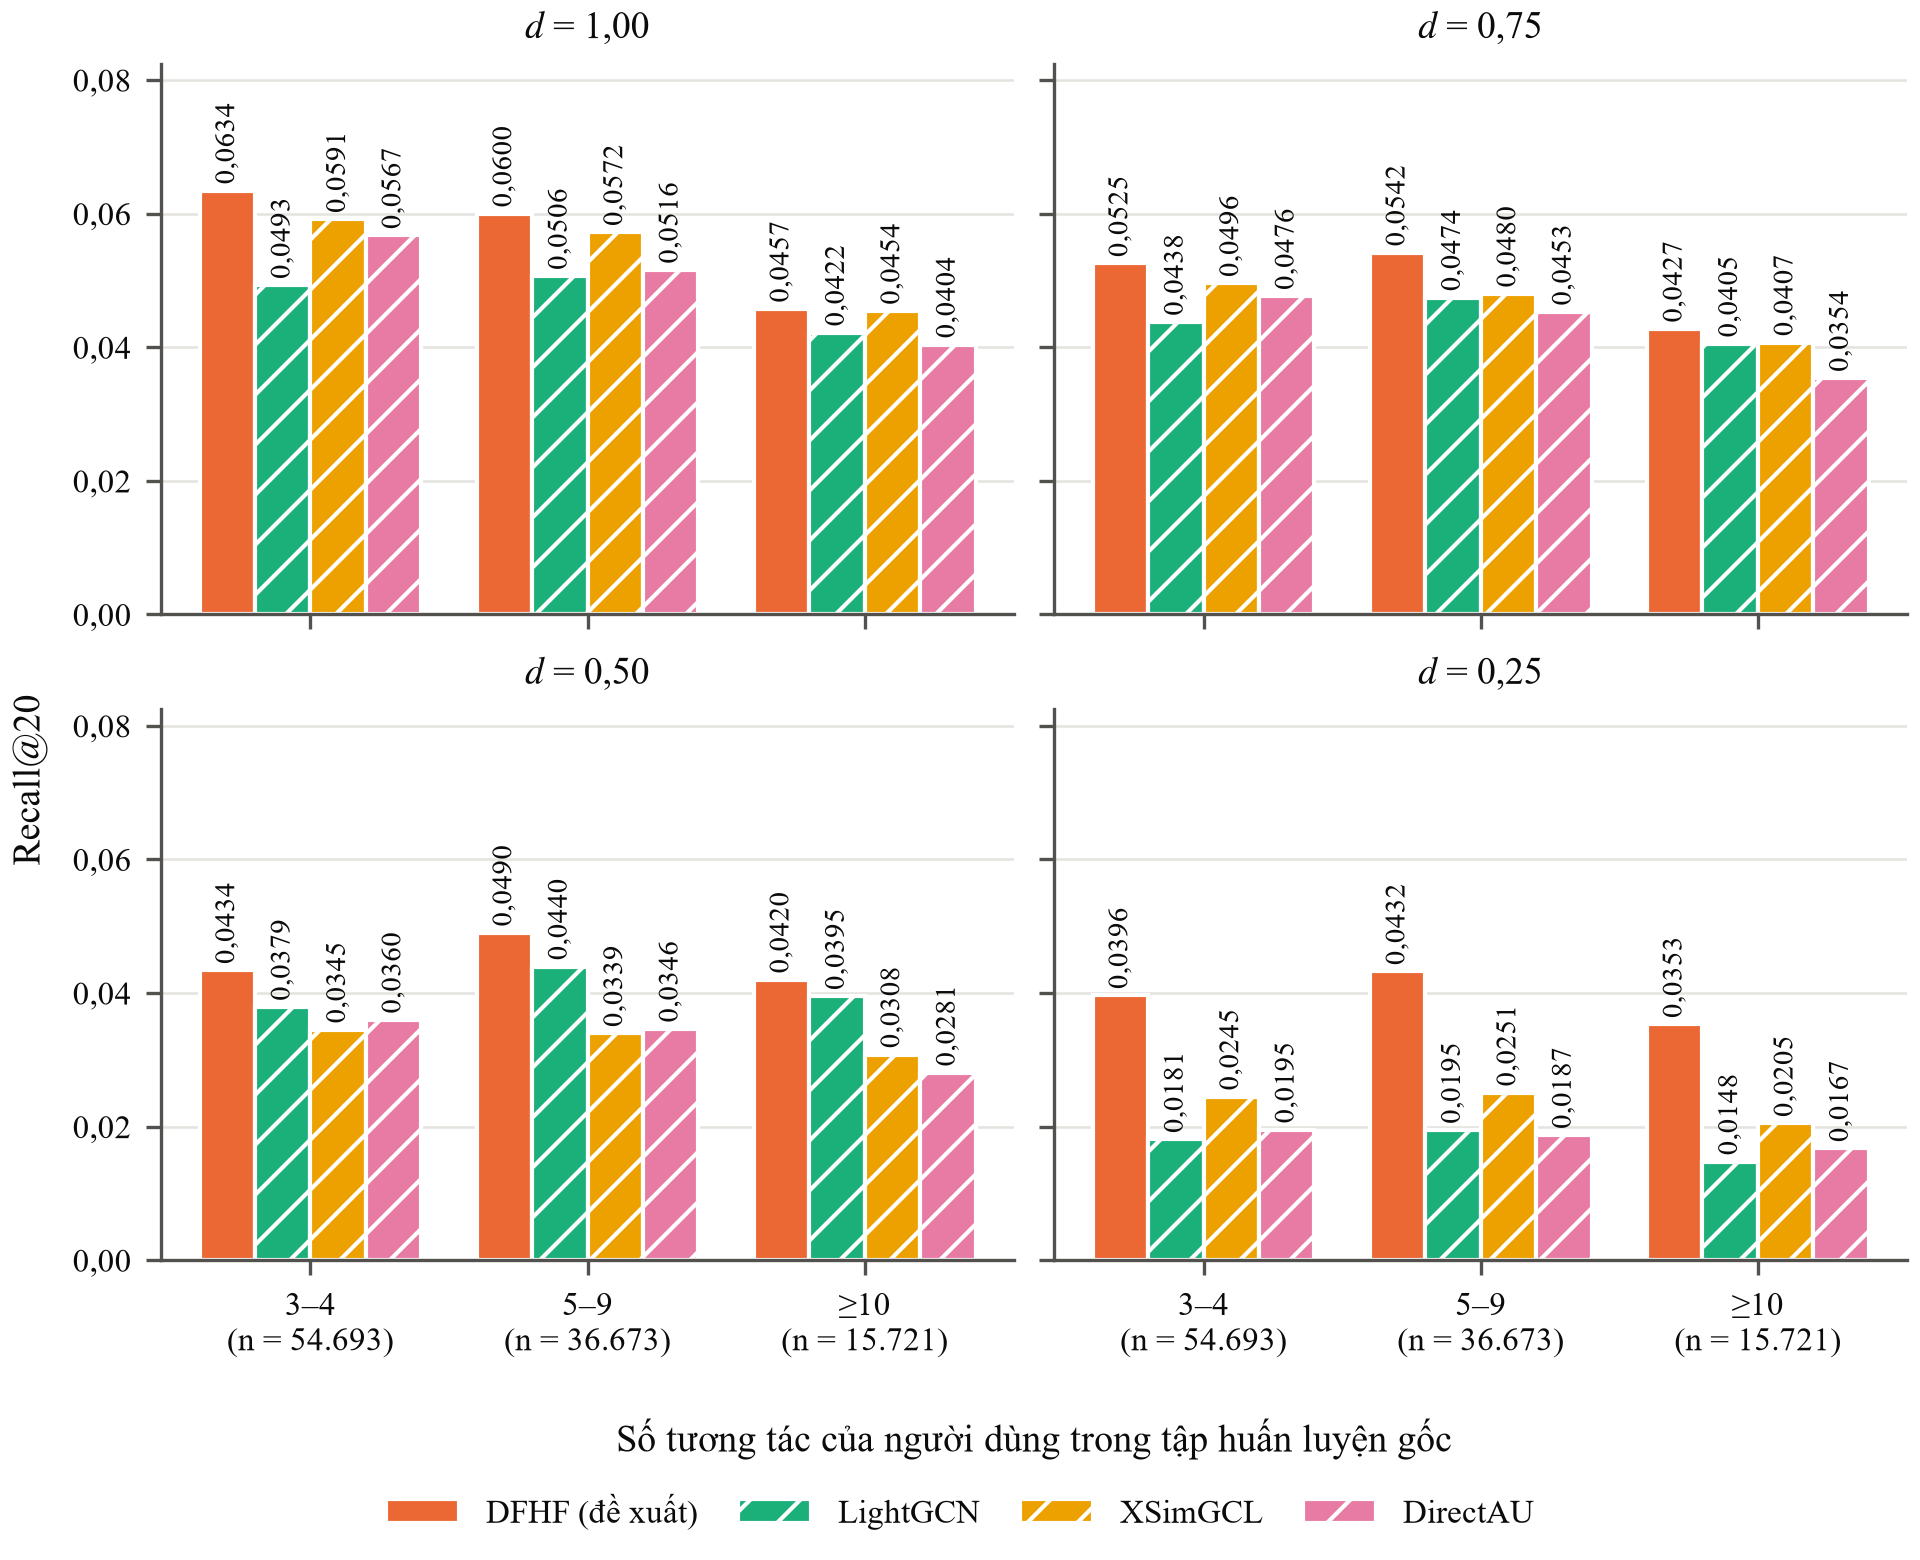
\includegraphics[width=0.68\linewidth]{H5_trained_user_groups_recall20.png}
\caption{Recall@20 theo độ dài lịch sử, nhóm cần huấn luyện}
\label{fig:trained-groups-recall20}
\end{figure}

\FloatBarrier
\subsubsection{Quá trình huấn luyện và chi phí tính toán}

Đường học ở \figref{fig:trained-curves} đo NDCG@20 trên tập xác thực sau mỗi epoch, cũng là đại lượng dùng để chọn checkpoint, nên các số trong mục này là số trên tập xác thực. Đường học chia nhóm thành hai kiểu hành vi. DFHF và XSimGCL học nhanh rồi quá khớp: khi có đủ dữ liệu, DFHF đạt đỉnh ở epoch 71 rồi giảm dần, đến epoch 200 thấp hơn đỉnh 24,5\%, còn XSimGCL đạt đỉnh sớm hơn, ở epoch 25, rồi giảm 21,4\%. LightGCN và DirectAU học chậm và gần như không giảm. Khi $d$ giảm, đỉnh của DFHF đến sớm hơn, ở epoch 66, 54 và 32; LightGCN, vốn đạt đỉnh ở epoch 169 khi $d=1$, đạt đỉnh ngay ở epoch 10 ở mức thưa nhất rồi giảm dần. XSimGCL vẫn đạt đỉnh quanh epoch 24--26 cho đến $d=0{,}5$, và ở epoch 6 ở mức thưa nhất. DirectAU thì ngược lại, đạt đỉnh gần cuối quá trình huấn luyện, cho thấy mô hình này có thể chưa hội tụ sau 200 epoch.

\begin{figure}[H]
\centering
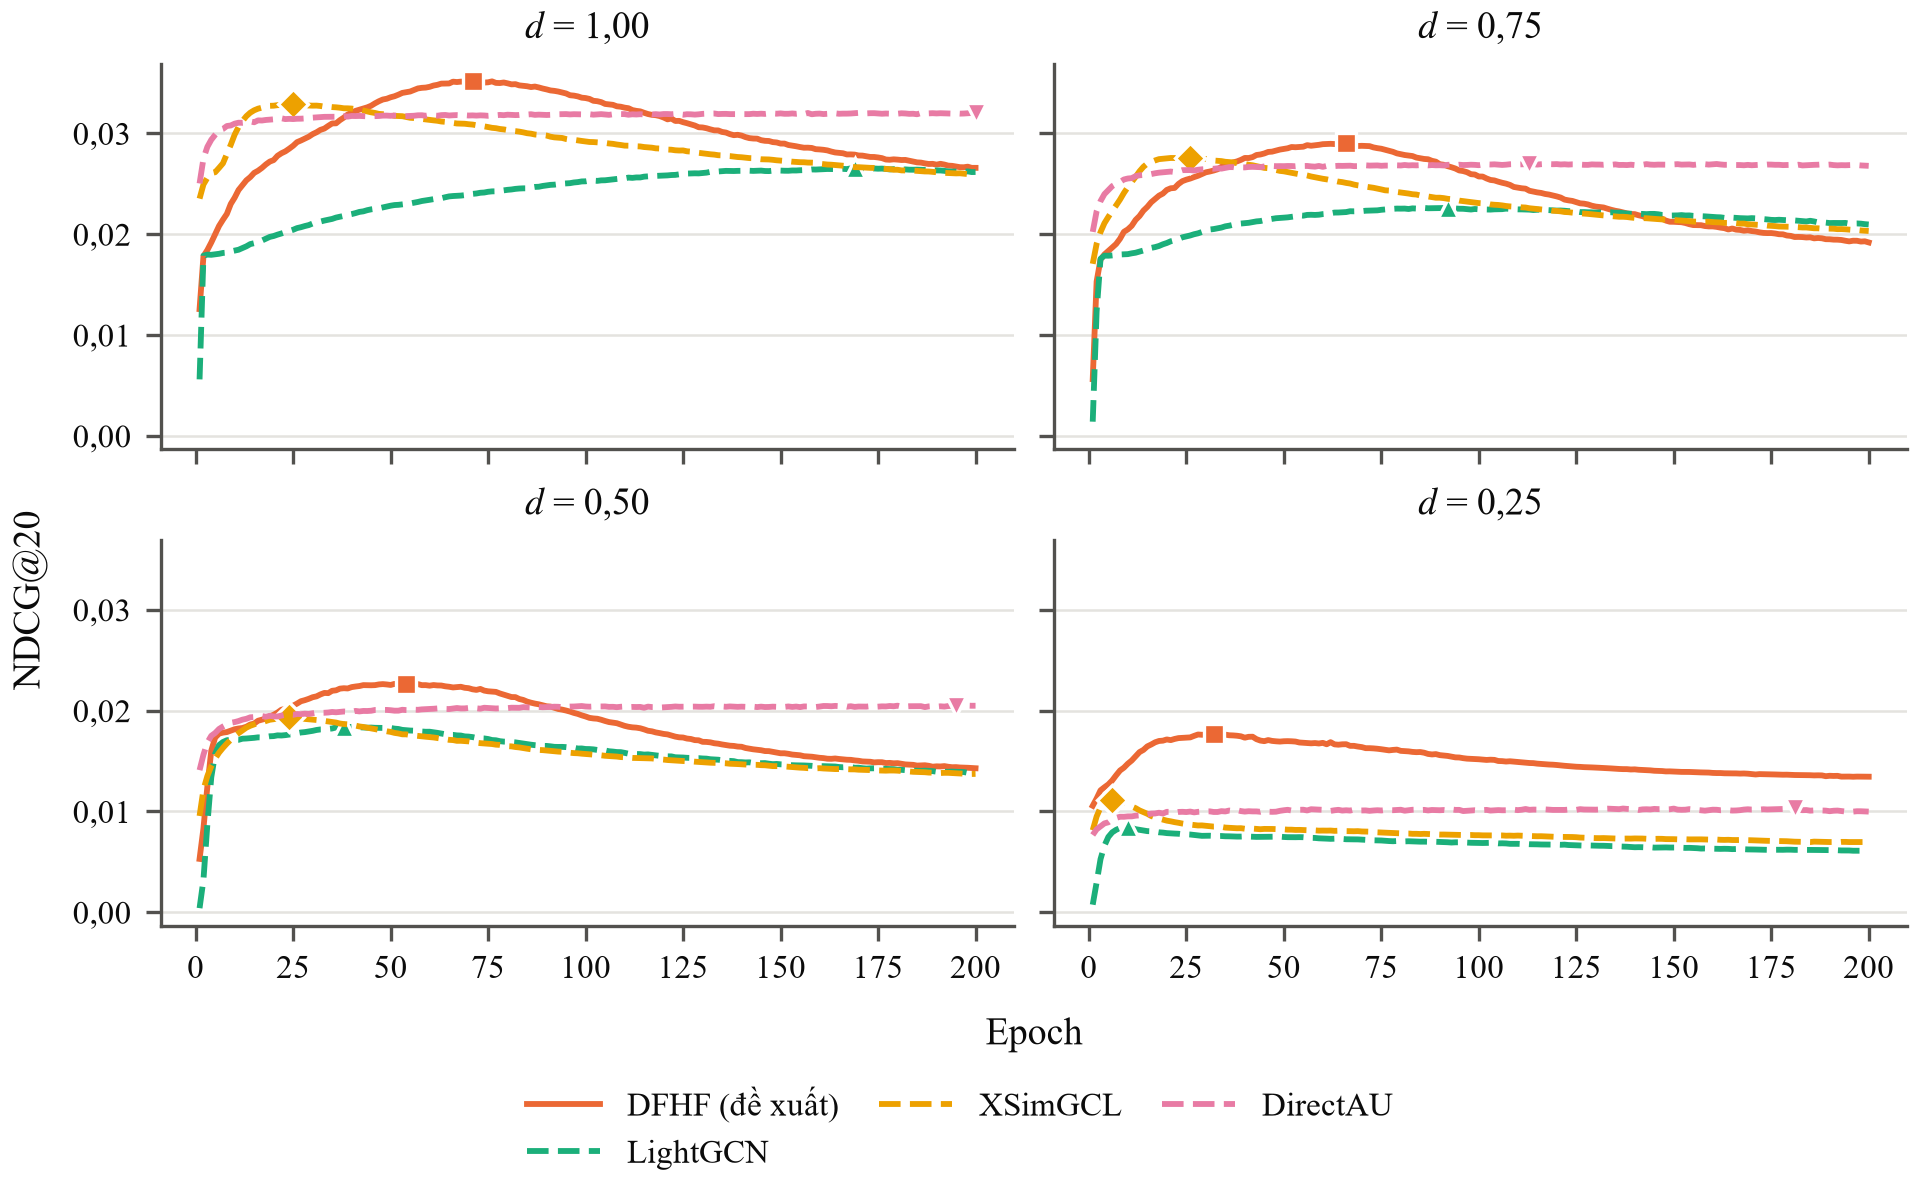
\includegraphics[width=0.75\linewidth]{H3_trained_learning_curves_ndcg20.png}
\caption{Đường học NDCG@20 trên tập xác thực, nhóm cần huấn luyện}
\label{fig:trained-curves}
\end{figure}

Đường học theo NDCG@10 ở \figref{fig:trained-curves-ndcg10} cho cùng hai kiểu hành vi; với DFHF và XSimGCL, epoch đạt đỉnh chỉ lệch không quá 4 epoch so với NDCG@20. Riêng DirectAU có đỉnh NDCG@10 đến sớm hơn nhiều, chẳng hạn epoch 98 so với 200 khi $d=1$, nhưng sau đỉnh đường gần như phẳng. Với DFHF, NDCG@10 ở epoch 200 thấp hơn đỉnh rõ rệt ở mọi mức, chẳng hạn từ 0,02946 xuống 0,02221 khi có đủ dữ liệu, nên dừng sớm có ích ở mọi mức.

\begin{figure}[H]
\centering
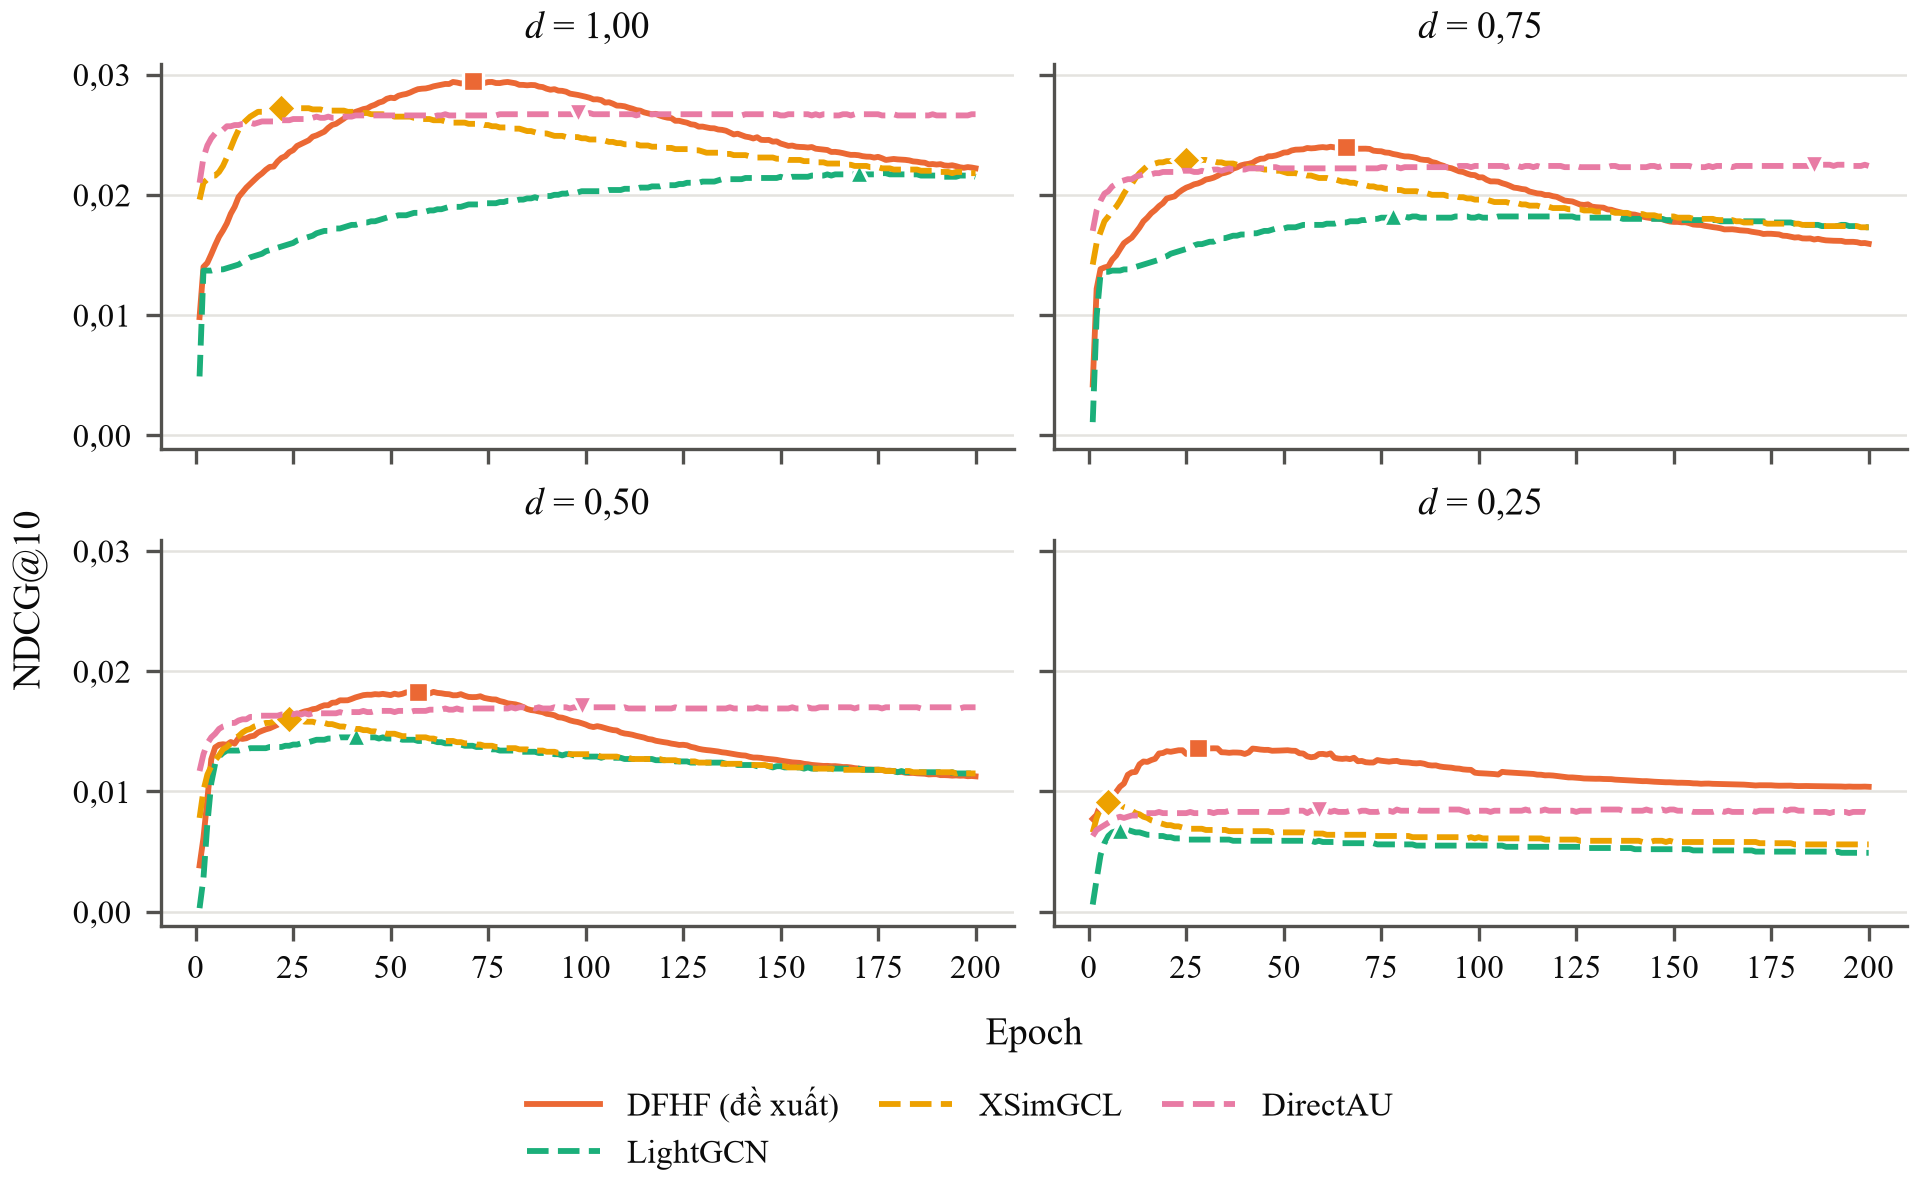
\includegraphics[width=0.75\linewidth]{H3_trained_learning_curves_ndcg10.png}
\caption{Đường học NDCG@10 trên tập xác thực, nhóm cần huấn luyện}
\label{fig:trained-curves-ndcg10}
\end{figure}


Hàm mất mát trên tập huấn luyện ở \figref{fig:trained-loss} cho thấy rõ hơn hiện tượng quá khớp: DFHF và XSimGCL tiếp tục giảm hàm mất mát sau khi NDCG trên tập xác thực đã qua đỉnh, nên tối ưu tốt hơn trên tập huấn luyện không bảo đảm chất lượng tốt hơn trên người dùng được đánh giá. Các ô con có trục tung riêng vì hàm mục tiêu khác nhau cả về thành phần lẫn thang giá trị, nên không thể so giá trị mất mát giữa các mô hình, và giá trị âm của DirectAU không phải lỗi tối ưu.

\begin{figure}[H]
\centering
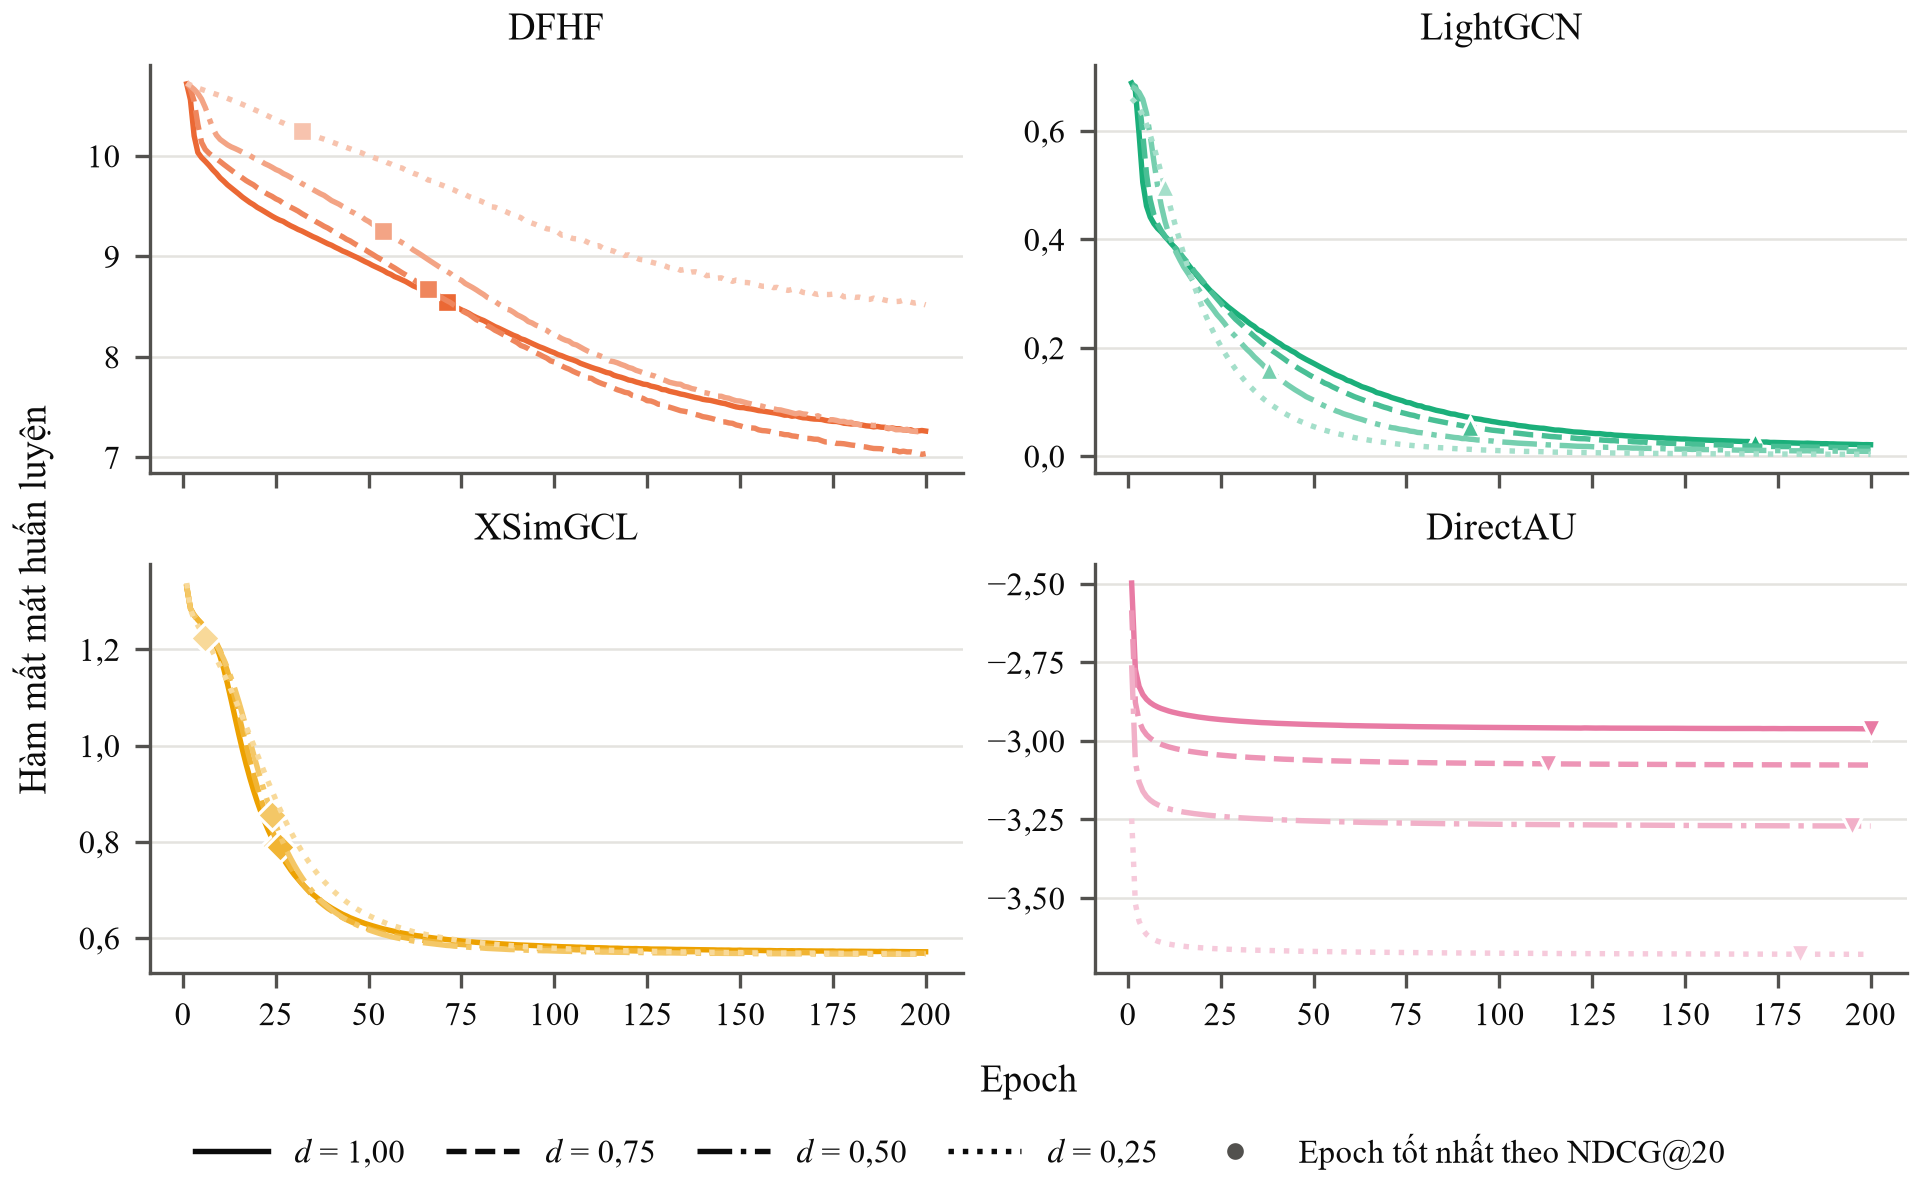
\includegraphics[width=0.75\linewidth]{H3c_loss.png}
\caption{Hàm mất mát huấn luyện, nhóm cần huấn luyện}
\label{fig:trained-loss}
\end{figure}

Điều này cho thấy dừng sớm là cần thiết với DFHF: trên tập xác thực, NDCG@20 của DFHF ở epoch 200 giảm còn 0,02658, trong khi checkpoint tốt nhất ở epoch 71 đạt 0,03519. \Tabref{tab:training} tổng hợp epoch được chọn, mức giảm sau đỉnh và thời gian mỗi epoch của cả bốn mô hình ở $d=1$, kèm NDCG@20 trên tập kiểm tra của checkpoint được chọn. Nhờ dừng sớm, DFHF được đánh giá ở epoch 71 và đạt 0,02724 trên tập kiểm tra, cao nhất nhóm; XSimGCL cũng được đánh giá ở epoch 25, trước khi quá khớp, và đạt 0,02561. Nếu lấy mô hình ở epoch cuối, hai mô hình này sẽ bị thiệt nhiều nhất, vì NDCG@20 trên tập xác thực của chúng đã giảm 24,5\% và 21,4\% so với đỉnh.

\begin{table}[H]
\centering
\small
\begin{tabular}{@{}lrrrrrr@{}}
\toprule
& & \multicolumn{3}{c}{NDCG@20 xác thực} & NDCG@20 & \\
\cmidrule(lr){3-5}
Mô hình & Epoch chọn & Chọn & Cuối & Giảm & kiểm tra & Giây/epoch \\
\midrule
DFHF & 71 & 0,03519 & 0,02658 & 24,5\% & 0,02724 & 37,9 \\
LightGCN & 169 & 0,02655 & 0,02617 & 1,4\% & 0,02168 & 11,2 \\
XSimGCL & 25 & 0,03292 & 0,02587 & 21,4\% & 0,02561 & 17,7 \\
DirectAU & 200 & 0,03205 & 0,03205 & 0\% & 0,02407 & 24,1 \\
\bottomrule
\end{tabular}
\caption[Huấn luyện và chi phí ($d=1$), nhóm cần huấn luyện]{Huấn luyện và chi phí ($d=1$), nhóm cần huấn luyện. NDCG@20 trên tập xác thực được đo tại checkpoint được chọn và tại epoch cuối; NDCG@20 trên tập kiểm tra là của checkpoint được chọn.}
\label{tab:training}
\end{table}

DFHF là mô hình chậm nhất nhóm: mỗi epoch mất 37,9 giây trên GPU Tesla T4, tổng khoảng 127 phút cho 200 epoch ở $d=1$, trong khi DirectAU, XSimGCL và LightGCN cần lần lượt 24,1, 17,7 và 11,2 giây mỗi epoch theo \tabref{tab:training}. Phần lớn chi phí đến từ softmax trên toàn danh mục và hai lần áp toán tử khuếch tán ở mỗi bước. Tuy vậy, đường học cho thấy phần lớn số epoch này là thừa: nếu dừng ở khoảng epoch 71, DFHF chỉ cần khoảng 45 phút, ít hơn 80 phút mà DirectAU cần cho 200 epoch. Đây chỉ là phép tính minh họa, vì điểm dừng phải được chọn trên một tập riêng và báo cáo chưa thử cách này.

Khi suy luận, cả bốn mô hình đều mất khoảng 0,01 ms cho mỗi người dùng khi chấm theo lô trên GPU Tesla T4. Điều này dễ hiểu vì cả bốn đều chấm điểm bằng tích vô hướng giữa vector người dùng và embedding sản phẩm. Chi phí thêm của DFHF vì vậy chỉ nằm ở giai đoạn huấn luyện. Đây là trung bình theo lô, không phải độ trễ của một dịch vụ thực tế.

Tóm lại, trên tập kiểm tra, DFHF có NDCG@20 cao nhất nhóm ở mọi mức dữ liệu, và là mô hình duy nhất của nhóm còn vượt MostPop ở $d=0{,}5$. Khi dữ liệu đủ dày, ưu thế này phù hợp với giả thuyết rằng một hàm mất mát gần thước đo xếp hạng có lợi. Khi dữ liệu thưa, ưu thế chủ yếu đến từ việc DFHF dựa vào hệ số chặn và đạt gần mốc độ phổ biến, thay vì cố cá nhân hóa từ một tương tác như các baseline. Đổi lại, DFHF huấn luyện chậm nhất nhóm và cần dừng sớm.

\FloatBarrier
\subsection{Hệ thống demo}
\label{sec:demo}

\subsubsection{Cài đặt môi trường và khởi động}

Ứng dụng được xây dựng bằng Streamlit, sử dụng dữ liệu đã xử lý và checkpoint của các mô hình để tạo gợi ý. Các lệnh cài đặt được thực hiện tại thư mục gốc của dự án. Trước hết, tạo và kích hoạt môi trường Python bằng Conda:

\begin{DemoCommand}
conda create -n AML python=3.11
conda activate AML
\end{DemoCommand}

Tiếp theo, cài các thư viện được khai báo trong \texttt{requirements.txt}:

\begin{DemoCommand}
python -m pip install -r requirements.txt
\end{DemoCommand}

Sau khi đã chuẩn bị dữ liệu và các checkpoint, khởi động ứng dụng bằng lệnh:

\begin{DemoCommand}
python -m streamlit run app/streamlit_app.py
\end{DemoCommand}

Người dùng mở địa chỉ hiển thị trong cửa sổ lệnh để truy cập giao diện. Ứng dụng nạp các mô hình đã lưu, không huấn luyện lại khi đổi người dùng hoặc tỉ lệ dữ liệu. Các bảng, biểu đồ và hình được đọc từ kết quả đã lưu trên tập kiểm tra, nên trùng với số liệu trong báo cáo. Gợi ý cho người dùng có sẵn theo đúng giao thức đánh giá trên tập kiểm tra: lịch sử đầu vào là các tương tác huấn luyện, sản phẩm của tập xác thực bị loại khỏi danh sách, và mười gợi ý đầu trùng với dự đoán đã lưu của từng mô hình.

\FloatBarrier
\subsubsection{Gợi ý cho người dùng có sẵn}

Thẻ ``Gợi ý cho khách'' cho phép chọn một người dùng trong danh sách hoặc nhấn ``Ngẫu nhiên'', sau đó chọn tỉ lệ tương tác huấn luyện được giữ lại. Bên trái là lịch sử tương tác và sản phẩm mục tiêu của tập kiểm tra; bên phải là 10 gợi ý đầu của bảy mô hình, mỗi mô hình một cột, thứ tự từ trên xuống tương ứng các hạng trong danh sách. Các cột được xếp theo hai nhóm như trong báo cáo: nhóm giải trực tiếp gồm GRNR, EASE và GF-CF, nhóm cần huấn luyện gồm DFHF, LightGCN, XSimGCL và DirectAU. Đầu mỗi cột ghi mô hình là đề xuất hay baseline và NDCG@20 của mô hình trên tập kiểm tra; cột EASE dùng bản top-128, vì ma trận đầy đủ không được lưu thành checkpoint. \Figref{fig:demo-existing} là màn hình của thẻ này với toàn bộ dữ liệu huấn luyện.

\begin{figure}[H]
\centering
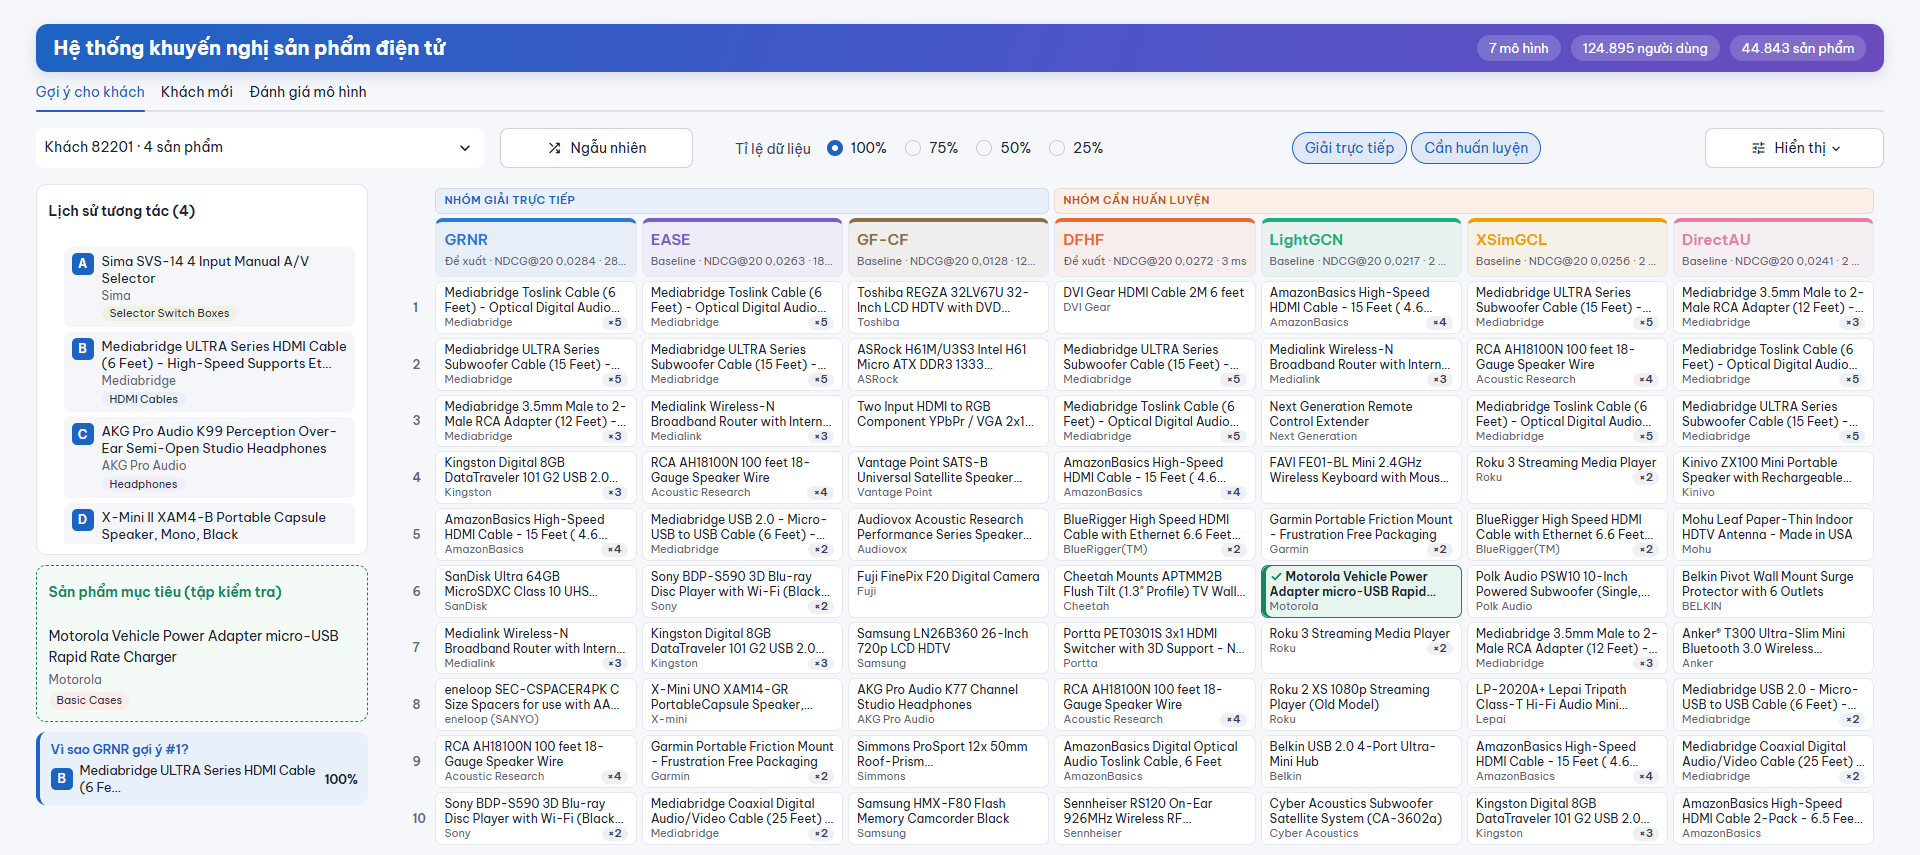
\includegraphics[width=\linewidth]{anh_1.png}
\caption{Giao diện gợi ý cho người dùng có sẵn}
\label{fig:demo-existing}
\end{figure}

Các nút ``Giải trực tiếp'' và ``Cần huấn luyện'' giúp thu gọn số cột cần xem. Nhãn $\times k$ cạnh sản phẩm cho biết có bao nhiêu mô hình đang hiển thị cùng gợi ý sản phẩm đó; khi rê chuột lên một sản phẩm chung, các ô tương ứng được làm sáng. Sản phẩm mục tiêu, nếu có trong danh sách, được tô xanh. Nút ``Hiển thị'' cho phép ẩn sản phẩm không rõ tên; bộ lọc này chỉ phục vụ giao diện và cần tắt khi đối chiếu danh sách với dự đoán đã lưu. Với GRNR, ô ``Vì sao GRNR gợi ý \#1?'' liệt kê các sản phẩm trong lịch sử có đóng góp dương vào gợi ý đầu tiên; phần này phản ánh các hệ số đã học, không xác nhận quan hệ nhân quả giữa sản phẩm.

Người dùng trong \figref{fig:demo-existing} có bốn sản phẩm trong lịch sử: một bộ chọn tín hiệu âm thanh--hình ảnh Sima, một cáp HDMI Mediabridge, một tai nghe AKG K99 và một loa di động X-Mini II; sản phẩm mục tiêu trên tập kiểm tra là một bộ sạc xe hơi micro-USB của Motorola. Chỉ LightGCN đưa bộ sạc này vào danh sách, ở hạng 6, nên chỉ một ô được tô xanh. Trường hợp này phản ánh đúng mức NDCG@20 khoảng 0,027--0,028 của các mô hình tốt nhất trên tập kiểm tra: với phần lớn người dùng, sản phẩm mục tiêu không nằm trong danh sách của mô hình nào, và việc một mô hình trúng ở một người dùng cụ thể không nói lên thứ hạng chung. Gợi ý đầu tiên của GRNR là một cáp quang Toslink cũng của Mediabridge, và ô giải thích cho thấy toàn bộ đóng góp dương đến từ chiếc cáp HDMI Mediabridge trong lịch sử. Nhiều sản phẩm được bốn đến năm mô hình cùng gợi ý, như cáp Toslink và cáp loa siêu trầm của Mediabridge, cáp HDMI của AmazonBasics hay dây loa RCA; đây đều là phụ kiện âm thanh--hình ảnh gắn với lịch sử của người dùng, nên các mô hình vẫn chia sẻ một phần danh sách dù dùng cơ chế khác nhau.

\FloatBarrier
\subsubsection{Gợi ý từ lịch sử nhập mới}

Ở thẻ ``Khách mới'', người dùng tìm sản phẩm theo từ khóa rồi nhấn ``Thêm'' để tạo lịch sử. \Figref{fig:demo-new} minh họa việc tìm bằng từ khóa ``Headphone'' và chọn một sản phẩm. GRNR, DFHF, EASE top-128 và GF-CF có thể chấm điểm lịch sử vừa nhập; ba baseline LightGCN, XSimGCL và DirectAU hiển thị thông báo không hỗ trợ khách mới vì các cài đặt này dùng embedding của người dùng đã có trong lúc huấn luyện. Tỉ lệ dữ liệu và bộ lọc hiển thị được dùng tiếp từ thẻ ``Gợi ý cho khách''.

\begin{figure}[H]
\centering
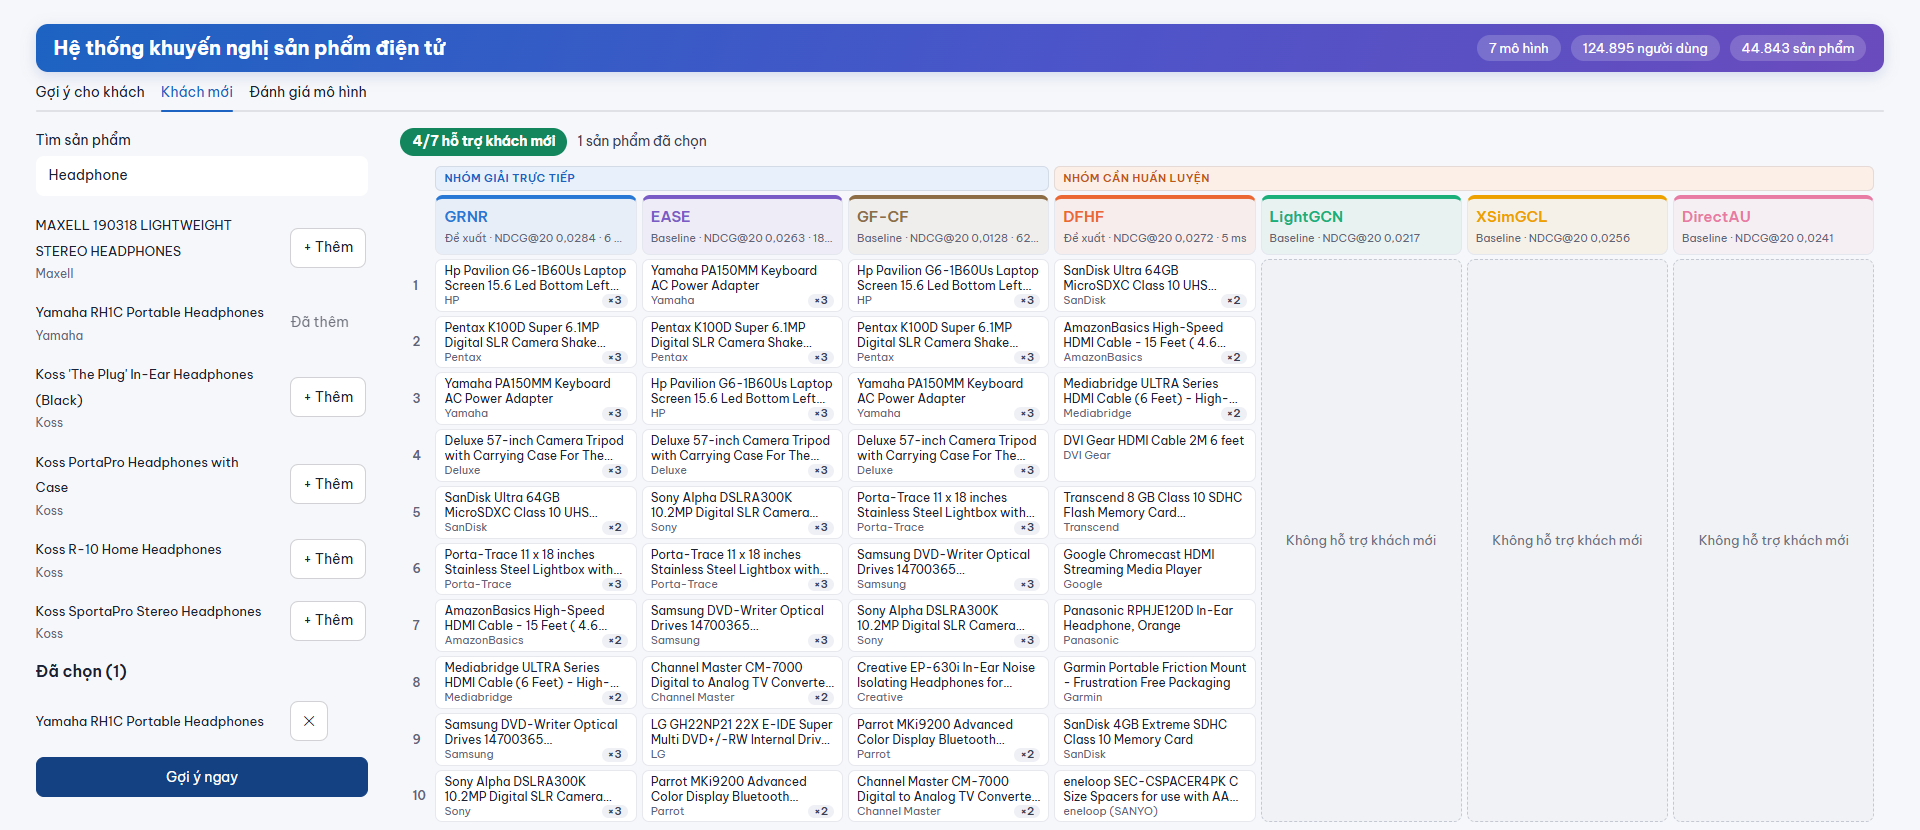
\includegraphics[width=\linewidth]{anh_2.png}
\caption{Tìm sản phẩm và tạo lịch sử cho người dùng mới}
\label{fig:demo-new}
\end{figure}

Trong \figref{fig:demo-new}, lịch sử chỉ gồm tai nghe Yamaha RH1C, và dòng ``4/7 hỗ trợ khách mới'' cho biết bốn mô hình trả về danh sách. Ba mô hình của nhóm giải trực tiếp cho danh sách gần giống nhau, với nhiều sản phẩm mang nhãn $\times 3$ như màn hình máy tính xách tay HP, máy ảnh Pentax hay chân máy ảnh Deluxe. Những sản phẩm này không cùng loại với tai nghe; chúng phản ánh đồng xuất hiện trong lịch sử của những người dùng đã tương tác với chiếc tai nghe này, đúng với cách ba mô hình xây toán tử sản phẩm--sản phẩm. Danh sách của DFHF khác hẳn, gồm thẻ nhớ SanDisk, cáp HDMI và các phụ kiện phổ biến khác. Lý do là lịch sử chỉ có một sản phẩm, nên với $\omega_1=0$ vector lịch sử bằng 0 và DFHF xếp hạng chỉ bằng hệ số chặn, cùng cơ chế đã phân tích với người dùng bậc 1 ở mục kết quả của nhóm cần huấn luyện.

Chức năng này minh họa khả năng nhận lịch sử mới mà không cần huấn luyện lại, chưa phải một phép đánh giá định lượng chất lượng gợi ý cho người dùng mới.

\FloatBarrier
\subsubsection{Tra cứu kết quả thực nghiệm}

Thẻ ``Đánh giá mô hình'' cho phép chọn tỉ lệ dữ liệu và thước đo cần tra cứu, rồi xem kết quả theo hai thẻ con ``Nhóm giải trực tiếp'' và ``Nhóm cần huấn luyện''. Mỗi thẻ con chỉ chứa mô hình đề xuất của nhóm đó cùng các baseline cùng nhóm, nên GRNR và DFHF không xuất hiện trong cùng một bảng so sánh. Nút ``Tải bảng kết quả (CSV)'' xuất bảng tổng hợp các lần chạy. Mục ``Tổng quan'' hiển thị các nhận xét tóm tắt, chỉ số xếp hạng và chi phí tính toán; \figref{fig:demo-overview} minh họa màn hình của nhóm giải trực tiếp khi giữ lại 25\% tương tác huấn luyện.

\begin{figure}[H]
\centering
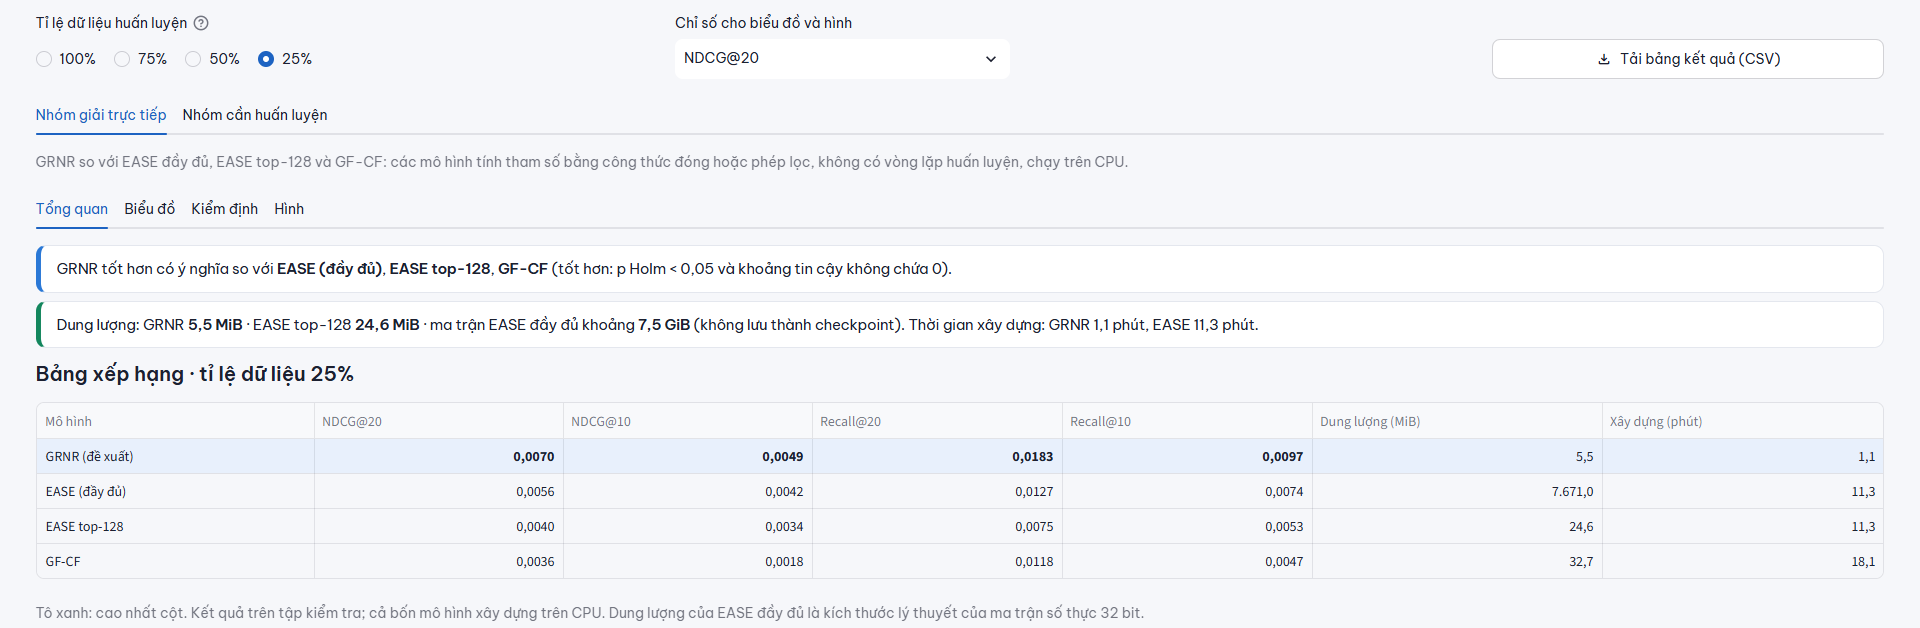
\includegraphics[width=\linewidth]{anh_4.png}
\caption{Màn hình tổng quan của nhóm giải trực tiếp tại tỉ lệ dữ liệu 25\%}
\label{fig:demo-overview}
\end{figure}

Ở mức này, GRNR có giá trị cao nhất nhóm ở cả bốn thước đo, với NDCG@20 bằng 0,00703 so với 0,00557 của EASE đầy đủ, và cao hơn có ý nghĩa thống kê so với cả ba baseline, đúng như \tabref{tab:closed-form}. Màn hình cũng đặt chất lượng cạnh chi phí: GRNR chiếm 5,5 MiB, EASE top-128 chiếm 24,6 MiB, còn ma trận của EASE đầy đủ khoảng 7,5 GiB.

Mục ``Biểu đồ'' thể hiện chất lượng theo tỉ lệ dữ liệu và chất lượng theo chi phí tại mức đang chọn, như ở \figref{fig:demo-charts}. Với nhóm giải trực tiếp, chi phí là dung lượng lưu trữ; với nhóm cần huấn luyện, chi phí là thời gian huấn luyện. Ở biểu đồ bên trái, ba mô hình hồi quy đi sát nhau trên toàn dải dữ liệu, còn GF-CF nằm thấp hẳn. Ở biểu đồ bên phải, trục dung lượng dùng thang log: tại 25\% dữ liệu, GRNR nằm ở góc trên bên trái, tức chất lượng cao nhất với dung lượng nhỏ nhất nhóm, còn EASE đầy đủ nằm tận cùng bên phải. Thời gian chạy cần được đọc cùng loại thiết bị ghi trên giao diện.

\begin{figure}[H]
\centering
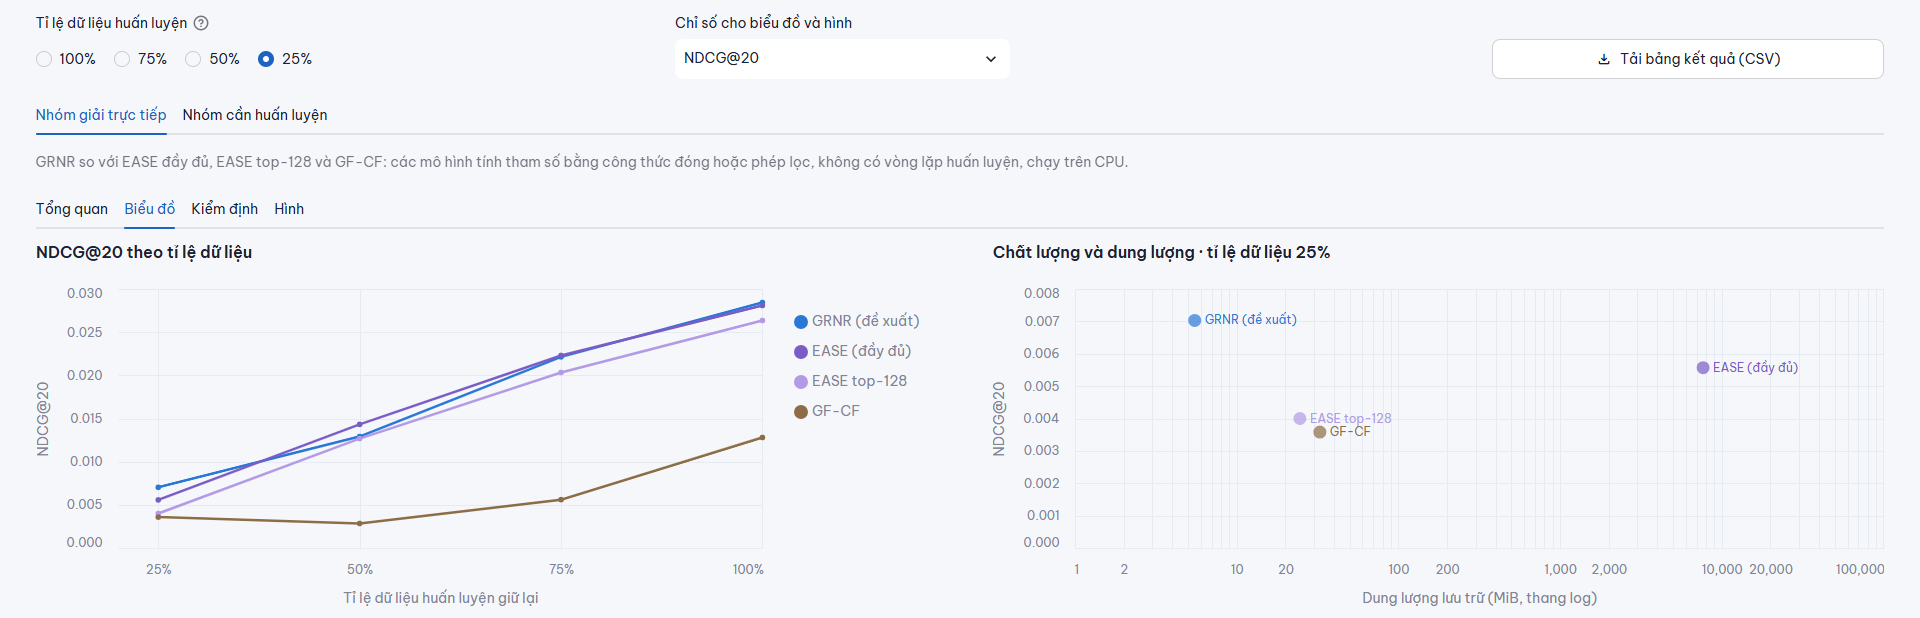
\includegraphics[width=\linewidth]{anh_5.png}
\caption{Biểu đồ chất lượng theo dữ liệu và theo dung lượng, nhóm giải trực tiếp}
\label{fig:demo-charts}
\end{figure}

Mục ``Kiểm định'' hiển thị, cho mô hình đề xuất của nhóm đang chọn so với từng baseline cùng nhóm, chênh lệch NDCG@20, khoảng tin cậy 95\%, giá trị $p$ một phía và giá trị sau hiệu chỉnh Holm trên 3 so sánh, theo đúng giao thức của báo cáo. \Figref{fig:demo-tests-full} là màn hình của nhóm cần huấn luyện khi giữ 100\% dữ liệu huấn luyện: DFHF cao hơn cả ba baseline với khoảng tin cậy không chứa 0 và $p_{\mathrm{Holm}}=0{,}0003$, đúng giá trị sàn đã nêu ở giao thức kiểm định; chênh lệch nhỏ nhất là so với XSimGCL, $+0{,}00163$.

\begin{figure}[H]
\centering
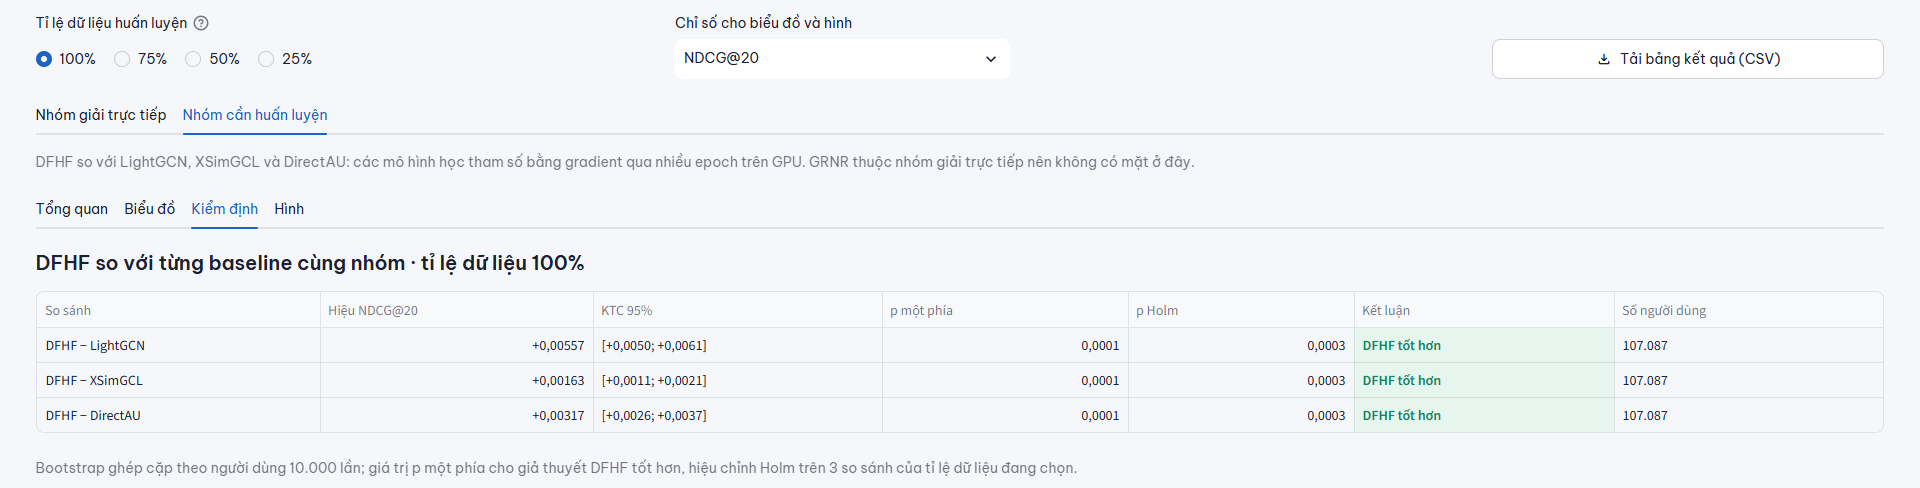
\includegraphics[width=\linewidth]{anh_3.png}
\caption{Màn hình kiểm định của nhóm cần huấn luyện tại tỉ lệ dữ liệu 100\%}
\label{fig:demo-tests-full}
\end{figure}

\Figref{fig:demo-tests-sparse} là cùng màn hình khi giữ 25\% dữ liệu huấn luyện. DFHF vẫn cao hơn cả ba baseline với $p_{\mathrm{Holm}}=0{,}0003$, và chênh lệch so với XSimGCL tăng lên $+0{,}00691$; như đã phân tích ở phần kết quả của nhóm này, ưu thế ở mức thưa chủ yếu đến từ người dùng chỉ còn một tương tác.

\begin{figure}[H]
\centering
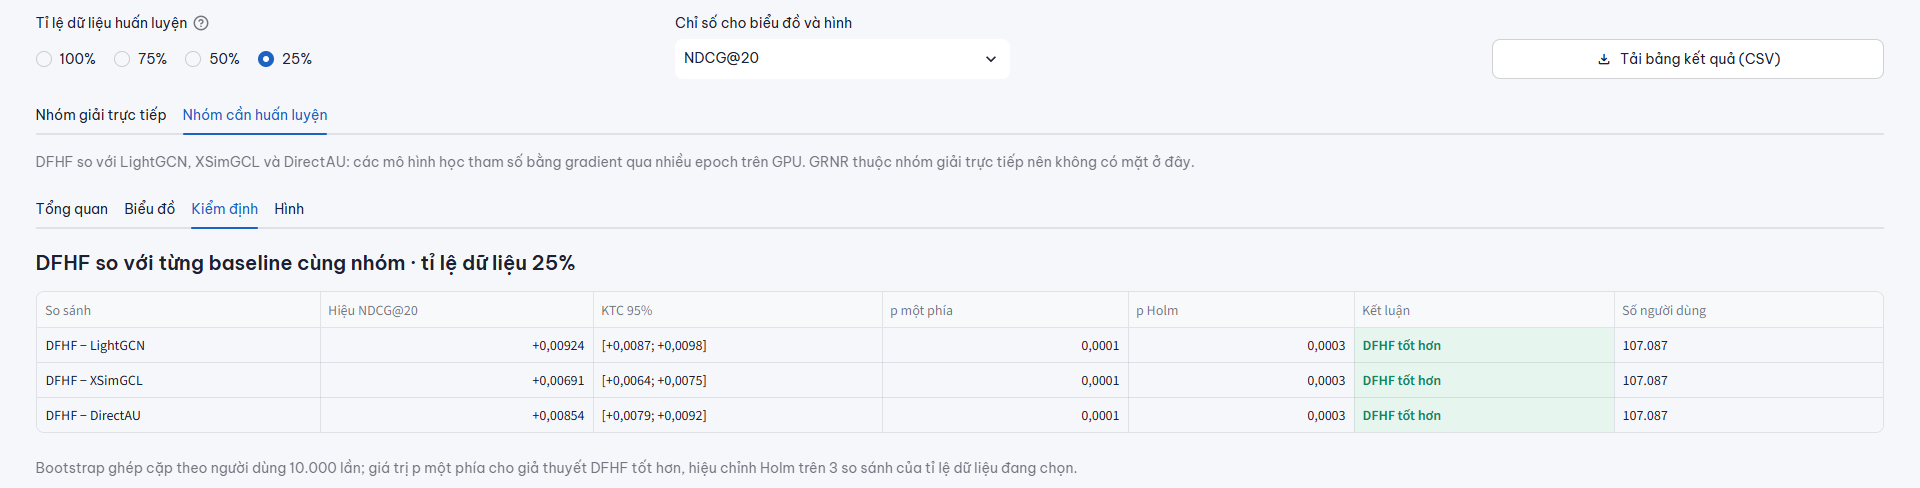
\includegraphics[width=\linewidth]{anh_6.png}
\caption{Màn hình kiểm định của nhóm cần huấn luyện tại tỉ lệ dữ liệu 25\%}
\label{fig:demo-tests-sparse}
\end{figure}

Mục ``Hình'' hiển thị chính các hình của báo cáo cho nhóm đang chọn và thước đo đang chọn, như ở \figref{fig:demo-gallery} với nhóm cần huấn luyện và NDCG@20. Các hình gồm chất lượng theo tỉ lệ dữ liệu, so sánh với MostPop, tỉ lệ duy trì, chất lượng theo độ dài lịch sử, NDCG@K, đường học và hàm mất mát; nhóm giải trực tiếp có thêm hình dung lượng lưu trữ. Đây chính là các tệp hình của báo cáo; riêng đường học và hàm mất mát được đo trên tập xác thực trong lúc huấn luyện. Các ảnh giao diện minh họa thao tác sử dụng; hệ thống chưa được đánh giá với người dùng thật, và thời gian phản hồi trong demo chưa đại diện cho độ trễ của một dịch vụ triển khai thực tế.

\begin{figure}[H]
\centering
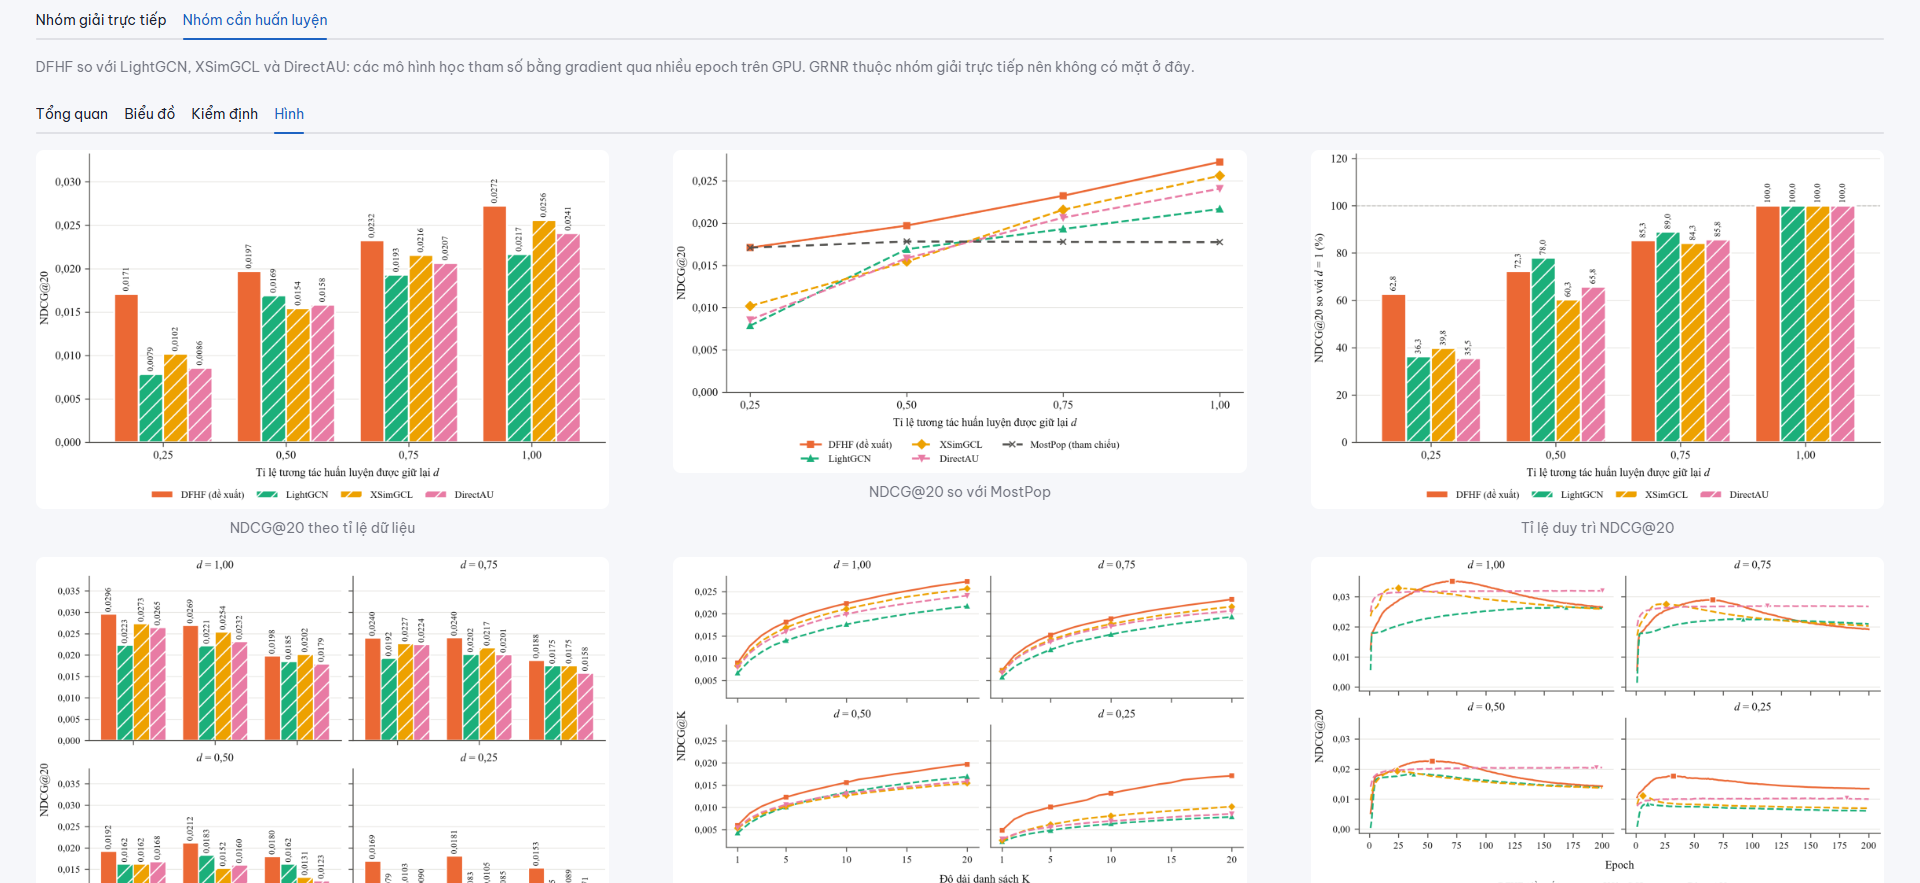
\includegraphics[width=\linewidth]{anh_7.png}
\caption{Thư viện hình của nhóm cần huấn luyện trong ứng dụng}
\label{fig:demo-gallery}
\end{figure}

\FloatBarrier

\subsection{Thảo luận và hạn chế}
\label{sec:discussion}

\FloatBarrier
\subsubsection{Hai chế độ dữ liệu}
 Đặt kết quả của hai nhóm cạnh nhau, dữ liệu này chia thành hai chế độ khá rõ.
\begin{itemize}
\item Khi dữ liệu còn dày, tức $d\ge0{,}75$, cá nhân hóa chiếm ưu thế. Mô hình tốt nhất của mỗi nhóm vượt MostPop 54--60\% ở $d=1$ và vẫn vượt 25--31\% ở $d=0{,}75$, và khác biệt giữa các mô hình có ý nghĩa thực tế.
\item Khi dữ liệu thưa, tức $d\le0{,}5$, tín hiệu cá nhân hóa gần như biến mất. Ở $d=0{,}5$, chỉ DFHF còn vượt MostPop, khoảng 11\%, còn mọi mô hình khác đã xuống dưới mốc này. Ở mức thưa nhất, không mô hình nào vượt MostPop, và DFHF chỉ còn ngang mốc.
\end{itemize}

Chuyển tiếp giữa hai chế độ trùng với hai thay đổi trong dữ liệu, thể hiện ở \tabref{tab:sparsity} và \tabref{tab:cooccurrence}: khi $d$ giảm từ 0,75 xuống 0,5, tỉ lệ người dùng chỉ còn một tương tác tăng từ 6\% lên 27\%, còn số cặp đồng xuất hiện giảm từ 56\% xuống 24\% so với ở $d=1$. Hai thay đổi này giải thích chung cho cả hai nhóm. Mô hình giải trực tiếp mất nguyên liệu, vì đồng xuất hiện cạn nhanh hơn số tương tác; mô hình cần huấn luyện mất ngữ cảnh, vì phần lớn người dùng không còn lịch sử để biểu diễn. Câu hỏi thứ hai, về độ thưa, vì thế có câu trả lời chủ yếu là âm tính: không mô hình nào trong báo cáo, kể cả hai mô hình đề xuất, khai thác được tín hiệu cá nhân hóa ở mức thưa nhất.

\FloatBarrier
\subsubsection{Khác biệt giữa tập xác thực và tập kiểm tra}

Kết quả trên tập kiểm tra thấp hơn rõ so với trên tập xác thực dùng để chọn mô hình. Khi có đủ dữ liệu, NDCG@20 của các mô hình cá nhân hóa trên tập kiểm tra chỉ bằng 72--82\% giá trị trên tập xác thực, trong khi MostPop vẫn giữ 98\%, nên mức vượt MostPop giảm khoảng một nửa. Sai lệch do chọn cấu hình không đủ giải thích mức giảm này, vì EASE đầy đủ và GF-CF không được chọn lại trên tập xác thực mà vẫn giảm 26\% và 32\%. Một giải thích hợp lý nằm ở giao thức đánh giá ở Mục~\ref{sec:evaluation-unit}: khi dự đoán tương tác cuối, mô hình không thấy tương tác áp cuối, vốn gần nhất về thời gian với lần tương tác cần đoán, còn MostPop không dùng lịch sử nên không chịu ảnh hưởng này. Ở mức thưa nhất, tỉ lệ giữa hai tập tăng lên 80--97\%, phù hợp với việc các mô hình khi đó dựa nhiều vào độ phổ biến. Nhóm chưa kiểm chứng giải thích này bằng một lần đánh giá có đưa tương tác áp cuối vào lịch sử.

Dù giá trị tuyệt đối giảm, thứ tự trong từng nhóm phần lớn giữ nguyên giữa hai tập: GRNR vẫn chưa phân biệt được với EASE đầy đủ khi dữ liệu dày, vẫn thua ở $d=0{,}5$ và thắng ở mức thưa nhất; DFHF vẫn dẫn nhóm ở cả bốn mức. Hai thay đổi đáng kể là GRNR không còn thua EASE top-128 ở $d=0{,}5$, và LightGCN thay DirectAU ở vị trí thứ hai của nhóm cần huấn luyện tại cùng mức. Cả hai đều xảy ra ở mức chuyển tiếp giữa hai chế độ dữ liệu, nơi các mô hình đứng sát nhau nhất, nên kết luận về thứ tự ở mức này cần được đọc thận trọng.

\FloatBarrier
\subsubsection{Ý nghĩa đối với từng mô hình đề xuất}
 Với GRNR, giá trị thực tế nằm ở chế độ dữ liệu dày. Tại đó, GRNR thay được EASE đầy đủ mà không có bằng chứng mất chất lượng, với dung lượng nhỏ hơn hai bậc, và tốt hơn cách đơn giản là cắt ma trận EASE. Ưu điểm này có ý nghĩa khi danh mục lớn đến mức ma trận đầy đủ không còn vừa bộ nhớ.

Với DFHF, giá trị nằm ở hai điểm. Thứ nhất, DFHF có điểm cao nhất nhóm ở mọi mức dữ liệu. Thứ hai, DFHF là mô hình duy nhất còn vượt MostPop ở $d=0{,}5$, và ở mức thưa nhất vẫn giữ được ngang mốc này thay vì rơi xuống dưới như các baseline. Điều này đến từ việc người dùng chỉ còn một tương tác được xếp hạng bằng hệ số chặn, dù chất lượng gần nhau chưa chứng minh thứ tự gợi ý giống MostPop. Một hệ thống thực tế có thể áp dụng cùng nguyên tắc cho bất kỳ mô hình nào: khi lịch sử quá ngắn, chuyển sang xếp hạng theo độ phổ biến.

\FloatBarrier
\subsubsection{Các giải thích cạnh tranh}
 Báo cáo chưa có thí nghiệm loại bỏ từng thành phần, nên các giải thích cơ chế đều là giả thuyết.
\begin{enumerate}[label=(\roman*)]
\item DFHF vượt các baseline cùng nhóm ở $d\ge0{,}5$ có thể nhờ softmax toàn danh mục, nhờ bộ lọc khuếch tán, hoặc nhờ cả hai. Muốn tách đóng góp của từng thành phần, cần thử DFHF với $F=I$ và với BPR thay cho softmax.
\item GRNR hơn EASE top-128 có thể nhờ ước lượng lại hệ số trên tập láng giềng, hoặc nhờ trọng số mẫu và điều chuẩn đồ thị. So GRNR với một biến thể không có điều chuẩn đồ thị sẽ tách được hai yếu tố này.
\item So sánh giữa GRNR và EASE đầy đủ đổi chiều theo $d$. Điều này có thể do giới hạn láng giềng có lợi khi rất thưa nhưng bó hẹp ở mức trung bình, hoặc chỉ là nhiễu của một lần lấy mẫu ở mỗi mức $d$. Chênh lệch ở $d=0{,}5$ cùng chiều trên cả hai tập, $-0{,}00202$ trên tập xác thực và $-0{,}00141$ trên tập kiểm tra, nhưng cả hai đều đo trên cùng một lần lấy mẫu dữ liệu huấn luyện; lặp lại việc lấy mẫu với nhiều seed mới cho biết chênh lệch này có ổn định hay không.
\item GRNR ít tệ nhất nhóm ở $d=0{,}25$ có thể vì mô hình dựa nhiều hơn vào hệ số chặn. Nhưng danh sách của GRNR khi đó lại gồm các sản phẩm ít phổ biến hơn so với ở $d=1$ theo \tabref{tab:closed-popularity}, trái với điều cách giải thích này dự đoán. Chấm điểm GRNR chỉ bằng hệ số chặn ở $d=0{,}25$, rồi so với mô hình đầy đủ, sẽ cho biết phần chất lượng còn lại đến từ đâu.
\end{enumerate}

\FloatBarrier
\subsubsection{Đối chiếu với tài liệu}

\begin{itemize}
\item Việc một xếp hạng theo độ phổ biến trở nên khó vượt khi dữ liệu thưa phù hợp với cảnh báo của Dacrema và cộng sự: các mô hình phức tạp thường không vượt được các phương pháp đơn giản được thiết lập cẩn thận~\cite{dacrema2019progress}.
\item EASE đầy đủ là đối thủ khó nhất của GRNR, phù hợp với nhận định của Steck rằng mô hình tuyến tính nông này là một baseline rất mạnh~\cite{steck2019ease}.
\item Dự án xếp hạng trên toàn bộ danh mục thay vì trên mẫu, nên tránh được sai lệch thứ tự do lấy mẫu mà Krichene và Rendle đã chỉ ra~\cite{krichene2020sampled}.
\item Dự án sử dụng tập xác thực để lựa chọn cấu hình và checkpoint, đồng thời đánh giá kết quả cuối cùng trên tập kiểm tra độc lập nhằm hạn chế sai lệch do lựa chọn mô hình~\cite{sun2020rigorous}.  Tuy nhiên, giao thức chia dữ liệu theo từng người dùng và thời gian chỉ chính xác đến ngày vẫn chưa bảo đảm một mốc thời gian toàn cục cho việc dự đoán tương lai~\cite{ji2023leakage}.
\end{itemize}

\FloatBarrier
\subsubsection{Hạn chế}
\label{sec:limitations}
 Các hạn chế được sắp theo loại mối đe dọa đối với kết luận.
\begin{enumerate}
\item Độ tin cậy nội tại.
  \begin{itemize}
  % \item Checkpoint và cấu hình được chọn trên chính tập xác thực dùng để báo cáo, nên mọi giá trị tuyệt đối đều lạc quan~\cite{cawley2010selection}.
  \item Checkpoint và cấu hình được lựa chọn dựa trên kết quả của tập xác thực, sau đó được cố định trước khi đánh giá trên tập kiểm tra độc lập. Quy trình này hạn chế sai lệch do lựa chọn mô hình trên cùng dữ liệu đánh giá.
  \item Ngân sách tinh chỉnh không cân bằng: GRNR và DFHF được tinh chỉnh trong quá trình phát triển, còn baseline dùng cấu hình cố định.
  \item DirectAU có dấu hiệu chưa hội tụ.
  \item GF-CF cho kết quả thấp bất thường và biến đổi không đều theo $d$, nên nhiều khả năng cấu hình hoặc cài đặt chưa phù hợp.
  \end{itemize}
\item Độ tin cậy thống kê.
  \begin{itemize}
  \item Mỗi mô hình và mỗi mức $d$ chỉ chạy một lần, nên khoảng tin cậy chỉ phản ánh biến động theo người dùng.
  \item Các phép kiểm định, nhất là của nhóm cần huấn luyện, được thiết kế sau khi đã xem kết quả trên tập xác thực, dù được áp dụng nguyên vẹn khi đánh giá trên tập kiểm tra.
  \item Phân tích theo nhóm người dùng và so sánh với MostPop chỉ mang tính mô tả, không hiệu chỉnh đa so sánh.
  \end{itemize}
\item Khả năng khái quát.
  \begin{itemize}
  \item Chỉ có một bộ dữ liệu.
  \item Bộ lọc 5-core làm dữ liệu nghiêng về người dùng và sản phẩm hoạt động nhiều.
  \item Thời gian chỉ chính xác đến ngày, và việc chia theo từng người dùng không có mốc thời gian chung, nên tập huấn luyện có thể chứa tương tác của người dùng khác xảy ra sau thời điểm cần dự đoán~\cite{ji2023leakage}; giao thức vì vậy không mô phỏng chặt chẽ việc dự đoán tương lai.
  \item Phần tổng quan tài liệu chỉ gồm các tài liệu nhóm đã đọc, không phải một tổng quan có hệ thống. Các phương pháp chỉ được nêu làm bối cảnh, gồm lọc cộng tác lân cận, SLIM, BSPM, Turbo-CF, PolyCF, FISM và Mult-VAE, không được chạy, nên chưa biết hai mô hình đề xuất đứng ở đâu so với chúng.
  \end{itemize}
\item Độ đúng của phép đo.
  \begin{itemize}
  \item Mỗi người dùng chỉ có một sản phẩm mục tiêu, nên một gợi ý phù hợp nhưng không trùng mục tiêu vẫn bị tính là sai.
  \item Khi đánh giá trên tập kiểm tra, tương tác của tập xác thực không được đưa vào lịch sử đầu vào và mô hình không được huấn luyện lại, nên giá trị tuyệt đối thấp hơn so với một hệ thống thực tế luôn dùng lịch sử mới nhất.
  \item Thời gian chạy được đo trên các máy khác nhau, nên chỉ mang tính tham khảo.
  \end{itemize}
\end{enumerate}

\clearpage
\section{Kết luận và hướng phát triển}
\label{sec:conclusion}

\subsection{Kết luận}

Báo cáo đã đề xuất và đánh giá hai mô hình khuyến nghị biểu diễn người dùng hoàn toàn bằng lịch sử tương tác, mỗi mô hình trong nhóm phương pháp của nó, trên bộ dữ liệu Amazon Electronics. Câu trả lời cho bốn câu hỏi nghiên cứu như sau.

Câu hỏi thứ nhất: chất lượng trong nhóm.
\begin{itemize}
\item Graph-Regularized Neighborhood Regression. Khi có đủ dữ liệu, GRNR có NDCG@20 cao nhất nhóm giải trực tiếp, 0,02843, nhưng chưa phân biệt được với EASE đầy đủ. Kết quả có ý nghĩa nhất là so với EASE top-128, mô hình có cùng ngân sách hệ số: GRNR tốt hơn ở ba trong bốn mức $d$, còn ở $d=0{,}5$ hai mô hình chưa phân biệt được. Khoảng cách lớn với GF-CF cần đọc thận trọng, vì baseline này có dấu hiệu chưa được thiết lập đúng.
\item Diffusion-Filtered History Factorization. DFHF có NDCG@20 cao nhất nhóm cần huấn luyện ở cả bốn mức $d$, đạt 0,02724 khi có đủ dữ liệu, và hơn cả ba baseline với khoảng tin cậy không chứa 0.
\end{itemize}

Câu hỏi thứ hai: ảnh hưởng của dữ liệu thưa. Đây là câu hỏi có câu trả lời chủ yếu là âm tính.
\begin{itemize}
\item Ở cả hai nhóm, phần chất lượng có được nhờ cá nhân hóa giảm nhanh khi bớt dữ liệu. Khi có đủ dữ liệu, mô hình tốt nhất mỗi nhóm vượt mốc độ phổ biến 54--60\%. Ở $d=0{,}5$, chỉ DFHF còn vượt mốc này. Ở mức thưa nhất, không mô hình nào vượt MostPop, và DFHF chỉ còn ngang mốc.
\item Với nhóm giải trực tiếp, báo cáo chỉ ra một nguyên nhân đo được: số cặp đồng xuất hiện giảm nhanh hơn nhiều so với số tương tác. Ở $d=0{,}25$, tập huấn luyện còn 25\% số tương tác nhưng chỉ còn 4,2\% số cặp đồng xuất hiện.
\item Ưu thế lớn của DFHF ở mức thưa nhất chủ yếu đến từ người dùng chỉ còn một tương tác: những người dùng này nhận vector lịch sử bằng 0 nên chỉ được xếp hạng bằng hệ số chặn, và đạt NDCG@20 gần mốc độ phổ biến, trong khi các baseline rơi xuống dưới mốc đó. Ưu thế này không phản ánh khả năng cá nhân hóa tốt hơn.
\item Giữa GRNR và EASE đầy đủ, kết quả không đơn điệu theo $d$, và EASE đầy đủ tốt hơn rõ ở $d=0{,}5$.
\end{itemize}

Câu hỏi thứ ba: chi phí.
\begin{itemize}
\item Ưu điểm rõ nhất của GRNR là dung lượng: checkpoint 40,5 MiB, so với khoảng 7.671 MiB của ma trận EASE đầy đủ, tức nhỏ hơn khoảng 190 lần. Khoảng cách này còn tăng theo quy mô danh mục, vì bộ nhớ của EASE tăng theo bình phương còn của GRNR tăng tuyến tính.
\item DFHF chậm nhất nhóm khi huấn luyện, với 37,9 giây mỗi epoch, nhưng thời gian suy luận cùng cỡ với các baseline. Đường học cho thấy phần lớn số epoch là thừa.
\item Số đo thời gian lẫn với khác biệt phần cứng, nên chỉ mang tính tham khảo.
\end{itemize}

Câu hỏi thứ tư: phục vụ lịch sử mới và giải thích. Cả hai mô hình đều chấm điểm được một lịch sử mới mà không cần huấn luyện lại. Hệ thống demo minh họa điều này, và hiển thị phân rã đại số của điểm GRNR thành đóng góp của từng sản phẩm trong lịch sử. Phân rã này là một mô tả trung thực về cách mô hình tính điểm, không phải một giải thích nhân quả về sở thích của người dùng. Hệ thống cũng chưa được đánh giá với người dùng thật.

Bài học chung.
\begin{itemize}
\item Trên dữ liệu này, khả năng cá nhân hóa phụ thuộc vào độ dày dữ liệu nhiều hơn vào lựa chọn mô hình.
\item Khi dữ liệu dày, hai mô hình đề xuất có khác biệt đo được so với baseline cùng nhóm. Việc giải thích khác biệt này bằng giới hạn láng giềng trong bài toán hoặc bằng hàm mất mát gần thước đo xếp hạng vẫn là giả thuyết, vì chưa có thí nghiệm loại bỏ thành phần.
\item Khi dữ liệu thưa, kết quả gợi ý rằng xếp hạng theo độ phổ biến cho lịch sử quá ngắn có lợi hơn cố cá nhân hóa từ một tương tác. Nhận định này chưa được kiểm tra bằng cách cho baseline dùng cùng phương án dự phòng.
\item So mọi mô hình với một mốc không cá nhân hóa là cần thiết. Thiếu mốc này, ưu thế của DFHF ở mức thưa nhất đã có thể bị hiểu sai.
\end{itemize}

Mọi kết luận trên được rút ra từ tập kiểm tra độc lập, sau khi cấu hình và checkpoint đã được chọn trên tập xác thực. Giá trị tuyệt đối trên tập kiểm tra thấp hơn trên tập xác thực khoảng một phần tư, nhưng thứ tự trong từng nhóm phần lớn giữ nguyên giữa hai tập. Phạm vi thực nghiệm vẫn giới hạn ở một bộ dữ liệu, một seed và ngân sách tinh chỉnh chưa cân bằng giữa mô hình đề xuất và baseline, nên các kết quả cần được kiểm chứng thêm trên nhiều bộ dữ liệu và nhiều lần chạy độc lập.


\subsection{Hướng phát triển}

Các hướng dưới đây được sắp theo mức độ ảnh hưởng đến độ tin cậy của kết luận.
\begin{enumerate}
% \item Xác nhận trên dữ liệu chưa dùng để chọn. Đánh giá các cấu hình đã khóa trên tập kiểm tra, hoặc trên một nửa tập xác thực chưa tham gia vào việc chọn. Việc này cho một ước lượng không bị nâng lạc quan, và cho biết ưu thế của DFHF có còn khi không được chọn checkpoint trên cùng tập hay không.
\item Đánh giá trong điều kiện triển khai thực tế. Mở rộng giao thức thực nghiệm sang đánh giá theo dòng thời gian với một mốc thời gian toàn cục, bảo đảm các tương tác được sử dụng để huấn luyện đều xảy ra trước thời điểm dự đoán. Đồng thời, đánh giá khả năng cập nhật lịch sử người dùng, độ trễ suy luận và chất lượng khuyến nghị trong điều kiện dữ liệu thay đổi liên tục. Hướng này giúp xác định mức độ phù hợp của GRNR và DFHF khi triển khai trong hệ thống thương mại điện tử thực tế.
\item Kiểm tra lại GF-CF và tinh chỉnh baseline cân bằng. Đối chiếu cài đặt GF-CF với kết quả đã công bố. Cho mọi baseline cùng ngân sách tinh chỉnh và đủ số epoch để hội tụ, đặc biệt là DirectAU.
\item Nhiều seed. Lặp lại việc huấn luyện và việc lấy mẫu tập huấn luyện để biết các chênh lệch nhỏ, như $-0{,}00141$ giữa GRNR và EASE đầy đủ ở $d=0{,}5$, có ổn định hay không.
\item Thí nghiệm loại bỏ thành phần.
  \begin{itemize}
  \item Với GRNR: bỏ điều chuẩn đồ thị, bỏ trọng số mẫu, và so với EASE được giải lại trên đúng tập láng giềng của GRNR.
  \item Với DFHF: thay bộ lọc bằng $F=I$, thay softmax bằng BPR, và gán trọng số khác 0 cho lịch sử đơn.
  \end{itemize}
  Mục tiêu là kiểm tra các giả thuyết cơ chế ở Mục~\ref{sec:discussion}.
\item Kết hợp có chủ đích với độ phổ biến. Từ phát hiện ở câu hỏi thứ hai, một hướng tự nhiên là chuyển sang xếp hạng theo độ phổ biến, hoặc trộn với nó, khi lịch sử quá ngắn, rồi đánh giá xem cách này có vượt được mốc MostPop ở mức thưa hay không.
\item Mở rộng dữ liệu. Thêm bộ dữ liệu khác, và thiết kế một đánh giá riêng cho người dùng mới thay cho thẻ minh họa trong ứng dụng demo.
\end{enumerate}

\clearpage
\phantomsection
\addcontentsline{toc}{section}{TÀI LIỆU THAM KHẢO}
% Mọi mục đã được đối chiếu với Crossref (mục có DOI) và arXiv (mục arXiv) ngày 11/11/2026.
\begin{thebibliography}{99}
\setlength{\itemsep}{2pt}

\bibitem{hu2008wmf}
Y.~Hu, Y.~Koren, C.~Volinsky.
\newblock Collaborative Filtering for Implicit Feedback Datasets.
\newblock In \emph{2008 Eighth IEEE International Conference on Data Mining (ICDM)}, trang 263--272, 2008.
\newblock DOI: \href{https://doi.org/10.1109/ICDM.2008.22}{10.1109/ICDM.2008.22}.

\bibitem{rendle2009bpr}
S.~Rendle, C.~Freudenthaler, Z.~Gantner, L.~Schmidt-Thieme.
\newblock BPR: Bayesian Personalized Ranking from Implicit Feedback.
\newblock In \emph{Proceedings of the 25th Conference on Uncertainty in Artificial Intelligence (UAI)}, 2009.
\newblock arXiv: \href{https://arxiv.org/abs/1205.2618}{1205.2618}.

\bibitem{koren2008factorization}
Y.~Koren.
\newblock Factorization Meets the Neighborhood: A Multifaceted Collaborative Filtering Model.
\newblock In \emph{Proceedings of the 14th ACM SIGKDD International Conference on Knowledge Discovery and Data Mining}, trang 426--434, 2008.
\newblock DOI: \href{https://doi.org/10.1145/1401890.1401944}{10.1145/1401890.1401944}.

\bibitem{ning2011slim}
X.~Ning, G.~Karypis.
\newblock SLIM: Sparse Linear Methods for Top-N Recommender Systems.
\newblock In \emph{2011 IEEE 11th International Conference on Data Mining (ICDM)}, trang 497--506, 2011.
\newblock DOI: \href{https://doi.org/10.1109/ICDM.2011.134}{10.1109/ICDM.2011.134}.

\bibitem{kabbur2013fism}
S.~Kabbur, X.~Ning, G.~Karypis.
\newblock FISM: Factored Item Similarity Models for Top-N Recommender Systems.
\newblock In \emph{Proceedings of the 19th ACM SIGKDD International Conference on Knowledge Discovery and Data Mining}, trang 659--667, 2013.
\newblock DOI: \href{https://doi.org/10.1145/2487575.2487589}{10.1145/2487575.2487589}.

\bibitem{mcauley2015image}
J.~McAuley, C.~Targett, Q.~Shi, A.~van den Hengel.
\newblock Image-Based Recommendations on Styles and Substitutes.
\newblock In \emph{Proceedings of the 38th International ACM SIGIR Conference on Research and Development in Information Retrieval}, trang 43--52, 2015.
\newblock DOI: \href{https://doi.org/10.1145/2766462.2767755}{10.1145/2766462.2767755}.

\bibitem{he2016ups}
R.~He, J.~McAuley.
\newblock Ups and Downs: Modeling the Visual Evolution of Fashion Trends with One-Class Collaborative Filtering.
\newblock In \emph{Proceedings of the 25th International Conference on World Wide Web (WWW)}, trang 507--517, 2016.
\newblock DOI: \href{https://doi.org/10.1145/2872427.2883037}{10.1145/2872427.2883037}.

\bibitem{liang2018multvae}
D.~Liang, R.~G. Krishnan, M.~D. Hoffman, T.~Jebara.
\newblock Variational Autoencoders for Collaborative Filtering.
\newblock In \emph{Proceedings of the 2018 World Wide Web Conference (WWW)}, trang 689--698, 2018.
\newblock DOI: \href{https://doi.org/10.1145/3178876.3186150}{10.1145/3178876.3186150}.

\bibitem{steck2019ease}
H.~Steck.
\newblock Embarrassingly Shallow Autoencoders for Sparse Data.
\newblock In \emph{The World Wide Web Conference (WWW)}, trang 3251--3257, 2019.
\newblock DOI: \href{https://doi.org/10.1145/3308558.3313710}{10.1145/3308558.3313710}.

\bibitem{dacrema2019progress}
M.~Ferrari~Dacrema, P.~Cremonesi, D.~Jannach.
\newblock Are We Really Making Much Progress? A Worrying Analysis of Recent Neural Recommendation Approaches.
\newblock In \emph{Proceedings of the 13th ACM Conference on Recommender Systems (RecSys)}, trang 101--109, 2019.
\newblock DOI: \href{https://doi.org/10.1145/3298689.3347058}{10.1145/3298689.3347058}.

\bibitem{he2020lightgcn}
X.~He, K.~Deng, X.~Wang, Y.~Li, Y.~Zhang, M.~Wang.
\newblock LightGCN: Simplifying and Powering Graph Convolution Network for Recommendation.
\newblock In \emph{Proceedings of the 43rd International ACM SIGIR Conference on Research and Development in Information Retrieval}, trang 639--648, 2020.
\newblock DOI: \href{https://doi.org/10.1145/3397271.3401063}{10.1145/3397271.3401063}.

\bibitem{krichene2020sampled}
W.~Krichene, S.~Rendle.
\newblock On Sampled Metrics for Item Recommendation.
\newblock In \emph{Proceedings of the 26th ACM SIGKDD International Conference on Knowledge Discovery \& Data Mining}, trang 1748--1757, 2020.
\newblock DOI: \href{https://doi.org/10.1145/3394486.3403226}{10.1145/3394486.3403226}.

\bibitem{sun2020rigorous}
Z.~Sun, D.~Yu, H.~Fang, J.~Yang, X.~Qu, J.~Zhang, C.~Geng.
\newblock Are We Evaluating Rigorously? Benchmarking Recommendation for Reproducible Evaluation and Fair Comparison.
\newblock In \emph{Fourteenth ACM Conference on Recommender Systems (RecSys)}, trang 23--32, 2020.
\newblock DOI: \href{https://doi.org/10.1145/3383313.3412489}{10.1145/3383313.3412489}.

\bibitem{shen2021gfcf}
Y.~Shen, Y.~Wu, Y.~Zhang, C.~Shan, J.~Zhang, K.~B. Letaief, D.~Li.
\newblock How Powerful is Graph Convolution for Recommendation?
\newblock In \emph{Proceedings of the 30th ACM International Conference on Information \& Knowledge Management (CIKM)}, trang 1619--1629, 2021.
\newblock DOI: \href{https://doi.org/10.1145/3459637.3482264}{10.1145/3459637.3482264}.

\bibitem{wang2022directau}
C.~Wang, Y.~Yu, W.~Ma, M.~Zhang, C.~Chen, Y.~Liu, S.~Ma.
\newblock Towards Representation Alignment and Uniformity in Collaborative Filtering.
\newblock In \emph{Proceedings of the 28th ACM SIGKDD Conference on Knowledge Discovery and Data Mining}, trang 1816--1825, 2022.
\newblock DOI: \href{https://doi.org/10.1145/3534678.3539253}{10.1145/3534678.3539253}.

\bibitem{ji2023leakage}
Y.~Ji, A.~Sun, J.~Zhang, C.~Li.
\newblock A Critical Study on Data Leakage in Recommender System Offline Evaluation.
\newblock \emph{ACM Transactions on Information Systems}, 41(3):75:1--75:27, 2023.
\newblock DOI: \href{https://doi.org/10.1145/3569930}{10.1145/3569930}.

\bibitem{yu2023xsimgcl}
J.~Yu, X.~Xia, T.~Chen, L.~Cui, N.~Q.~V. Hung, H.~Yin.
\newblock XSimGCL: Towards Extremely Simple Graph Contrastive Learning for Recommendation.
\newblock \emph{IEEE Transactions on Knowledge and Data Engineering}, 2023.
\newblock DOI: \href{https://doi.org/10.1109/TKDE.2023.3288135}{10.1109/TKDE.2023.3288135}.

\bibitem{choi2023bspm}
J.~Choi, S.~Hong, N.~Park, S.-B.~Cho.
\newblock Blurring-Sharpening Process Models for Collaborative Filtering.
\newblock In \emph{Proceedings of the 46th International ACM SIGIR Conference on Research and Development in Information Retrieval (SIGIR)}, trang 1096--1106, 2023.
\newblock DOI: \href{https://doi.org/10.1145/3539618.3591645}{10.1145/3539618.3591645}.

\bibitem{park2024turbocf}
J.-D.~Park, Y.-M.~Shin, W.-Y.~Shin.
\newblock Turbo-CF: Matrix Decomposition-Free Graph Filtering for Fast Recommendation.
\newblock In \emph{Proceedings of the 47th International ACM SIGIR Conference on Research and Development in Information Retrieval (SIGIR)}, trang 2672--2676, 2024.
\newblock DOI: \href{https://doi.org/10.1145/3626772.3657916}{10.1145/3626772.3657916}.

\bibitem{wu2024sampledsoftmax}
J.~Wu, X.~Wang, X.~Gao, J.~Chen, H.~Fu, T.~Qiu.
\newblock On the Effectiveness of Sampled Softmax Loss for Item Recommendation.
\newblock \emph{ACM Transactions on Information Systems}, 42(4):98:1--98:26, 2024.
\newblock DOI: \href{https://doi.org/10.1145/3637061}{10.1145/3637061}.

\bibitem{hoerl1970ridge}
A.~E. Hoerl, R.~W. Kennard.
\newblock Ridge Regression: Biased Estimation for Nonorthogonal Problems.
\newblock \emph{Technometrics}, 12(1):55--67, 1970.
\newblock DOI: \href{https://doi.org/10.1080/00401706.1970.10488634}{10.1080/00401706.1970.10488634}.

\bibitem{shuman2013graph}
D.~I. Shuman, S.~K. Narang, P.~Frossard, A.~Ortega, P.~Vandergheynst.
\newblock The Emerging Field of Signal Processing on Graphs: Extending High-Dimensional Data Analysis to Networks and Other Irregular Domains.
\newblock \emph{IEEE Signal Processing Magazine}, 30(3):83--98, 2013.
\newblock DOI: \href{https://doi.org/10.1109/MSP.2012.2235192}{10.1109/MSP.2012.2235192}.

\bibitem{oord2018cpc}
A.~van den Oord, Y.~Li, O.~Vinyals.
\newblock Representation Learning with Contrastive Predictive Coding.
\newblock arXiv:1807.03748, 2018.
\newblock \url{https://arxiv.org/abs/1807.03748}.


\bibitem{boyd2004convex}
S.~Boyd, L.~Vandenberghe.
\newblock \emph{Convex Optimization}.
\newblock Cambridge University Press, 2004.
\newblock DOI: \href{https://doi.org/10.1017/CBO9780511804441}{10.1017/CBO9780511804441}.

\bibitem{chung1997spectral}
F.~R.~K. Chung.
\newblock \emph{Spectral Graph Theory}.
\newblock CBMS Regional Conference Series in Mathematics, tập 92. American Mathematical Society, 1997.
\newblock DOI: \href{https://doi.org/10.1090/cbms/092}{10.1090/cbms/092}.

\bibitem{cawley2010selection}
G.~C. Cawley, N.~L.~C. Talbot.
\newblock On Over-fitting in Model Selection and Subsequent Selection Bias in Performance Evaluation.
\newblock \emph{Journal of Machine Learning Research}, 11:2079--2107, 2010.
\newblock \url{https://jmlr.org/papers/v11/cawley10a.html}.

\bibitem{qin2025polycf}
Y.~Qin, W.~Ju, Y.~Gu, Z.~Qiao, Z.~Xiao, M.~Zhang.
\newblock PolyCF: Towards Optimal Spectral Graph Filters for Collaborative Filtering.
\newblock \emph{ACM Transactions on Information Systems}, 43(4):94:1--94:28, 2025.
\newblock DOI: \href{https://doi.org/10.1145/3728464}{10.1145/3728464}.

\bibitem{sarwar2001itembased}
B.~Sarwar, G.~Karypis, J.~Konstan, J.~Riedl.
\newblock Item-Based Collaborative Filtering Recommendation Algorithms.
\newblock In \emph{Proceedings of the 10th International Conference on World Wide Web (WWW)}, trang 285--295, 2001.
\newblock DOI: \href{https://doi.org/10.1145/371920.372071}{10.1145/371920.372071}.

\bibitem{koren2009mf}
Y.~Koren, R.~Bell, C.~Volinsky.
\newblock Matrix Factorization Techniques for Recommender Systems.
\newblock \emph{Computer}, 42(8):30--37, 2009.
\newblock DOI: \href{https://doi.org/10.1109/MC.2009.263}{10.1109/MC.2009.263}.

\bibitem{kingma2015adam}
D.~P.~Kingma, J.~Ba.
\newblock Adam: A Method for Stochastic Optimization.
\newblock In \emph{International Conference on Learning Representations (ICLR)}, 2015.
\newblock arXiv: \href{https://arxiv.org/abs/1412.6980}{1412.6980}.

\bibitem{rendle2019metrics}
S.~Rendle.
\newblock Evaluation Metrics for Item Recommendation under Sampling.
\newblock arXiv:1912.02263, 2019.
\newblock \url{https://arxiv.org/abs/1912.02263}.

\bibitem{jarvelin2002cumulated}
K.~Järvelin, J.~Kekäläinen.
\newblock Cumulated Gain-Based Evaluation of IR Techniques.
\newblock \emph{ACM Transactions on Information Systems}, 20(4):422--446, 2002.
\newblock DOI: \href{https://doi.org/10.1145/582415.582418}{10.1145/582415.582418}.

\end{thebibliography}


\end{document}
